\documentclass[11pt,leqno]{amsbook}

% This codes produces an error if some include file is not founded
\makeatletter
\def\mkfilename#1{%
  \if\relax\detokenize\expandafter{#1}\relax\else#1/\fi}
\AddToHook{include/before}%
  {\IfFileExists{\mkfilename\CurrentFilePath\CurrentFile}{}
     {\GenericError{}{Error: File \mkfilename\CurrentFilePath\CurrentFile.tex not found!}{\@gobble}{}}}
\makeatother


\usepackage{graphicx}
\usepackage[utf8]{inputenc}
\usepackage[spanish,es-nodecimaldot]{babel}
\usepackage{t1enc}
\usepackage{color}
\usepackage{multicol}
\usepackage{tcolorbox}
\usepackage{amsthm}
\usepackage{amsmath}
\usepackage{amssymb}
\usepackage{bm}
\usepackage{framed}
\definecolor{shadecolor}{RGB}{248,248,248}
\newenvironment{Shaded}{\begin{snugshade}}{\end{snugshade}}

\usepackage{savesym}
\savesymbol{tcc}  % tcc está definido en algún otro paquete
%\usepackage[ruled,vlined]{algorithm2e}
\restoresymbol{TXF}{tcc}

\usepackage{hyperref}
\makeatletter
\pdfstringdefDisableCommands{\let\bm\@firstofone}
\makeatother

\usepackage{listings}
\renewcommand{\ttdefault}{pcr}
\lstset{
emph={row_echelon},
emphstyle={\bfseries},
breaklines=true,
basicstyle=\ttfamily,
columns=fullflexible,
keepspaces=true,
showspaces=false,
showstringspaces=false,
inputencoding=utf8,
literate=%
         {á}{{\'a}}1
         {é}{{\'e}}1
         {í}{{\'i}}1
         {ó}{{\'o}}1
         {ú}{{\'u}}1
         {ñ}{{\~n}}1
}

\usepackage{xspace}
\usepackage{graphicx}
\graphicspath{ {./imagenes/} }

%\usepackage{breqn}   %% OJO NO COMPILA!



\vsize=27.9cm \hsize=21cm \setlength{\textwidth}{16cm}
\setlength{\textheight}{21.5cm}
\setlength{\oddsidemargin}{0.0cm}
\setlength{\evensidemargin}{0.0cm}
%\setlength{\topmargin}{-1.5cm}
\parskip 5pt

\newtheoremstyle{noind}{6pt}{6pt}{}{}{\scshape}{.}{.5em}{}

\theoremstyle{noind}
%\theoremstyle{plain}
\newtheorem{teo}{Teorema}[chapter]
\newtheorem{lema}{Lema}[chapter]
\newtheorem{prop}{Proposici\'on}[chapter]
\newtheorem{cor}{Corolario}[chapter]
\newtheorem{coro}{Corolario}[chapter]
\newtheorem{remark}{Observaci\'on}[chapter]
\newtheorem{rem}{Observaci\'on}[chapter]

\newtheoremstyle{def2}{6pt}{6pt}{}{}{\scshape}{.}{.5em}{}
\theoremstyle{def2}
\newtheorem{ejemplo}{Ejemplo}[chapter]
\newtheorem{aplicacion}{Aplicaci\'on}[chapter]
\newtheorem{defi}{Definici\'on}[chapter]
\newtheorem{ej}{Ejercicio}[chapter] %numera os 'Ejercicios' reseteando
\newtheorem{ejercicio}{Ejercicio}[chapter] %numera os 'Ejercicios' reseteando
%en cada 'capítulo'.
%\newtheorem{ej}{Ejercicio}[section] %numera os 'Ejercicios' reseteando
%en cada 'capítulo'.


%% User definitions:
%\newcommand{\texorpdfstring}[2]{#1}

\renewcommand{\theequation}{\arabic{chapter}.\arabic{equation}}
\newcommand{\beq}{\begin{equation}}
\newcommand{\eeq}{\end{equation}}
\newcommand{\tcc}{\begin{tcolorbox}[colback=black!15!white,colframe=black!75!black]}
%\newcommand{\tcc}{\begin{tcolorbox}[colframe=black!75!black]}

\newcommand{\tccdefi}{\begin{tcolorbox}
[colback=blue!15!white,colframe=black!75!black]}

\newcommand{\etcc}{\end{tcolorbox}}

\newcommand{\si}{\sigma}
\newcommand{\al}{\alpha}
\newcommand{\be}{\beta}
\newcommand{\Om}{\Omega}
\newcommand{\la}{\lambda}
\newcommand{\noi}{\noindent}
\newcommand{\di}{\displaystyle}
\newcommand{\sen}{\mbox{sen\,}}
\newcommand{\B}{\mathcal B}
\newcommand{\E}{\mathcal E}
\newcommand{\R}{\mathbb R}

\newcommand{\K}{\mathbb K}
\newcommand{\Kn}{\K^{n}}
\newcommand{\Kmn}{\K^{m\times n}}
\newcommand{\Knn}{\K^{n\times n}}

\newcommand{\Cm}{\C^{m}}
\newcommand{\Rmm}{\R^{m\times m}}
\newcommand{\Cmm}{\C^{m\times m}}
\newcommand{\Rm}{\R^{m}}
\newcommand{\Cmn}{\C^{m\times n}}

\newcommand{\N}{\mathbb N}
\newcommand{\Z}{\mathbb Z}
\newcommand{\LL}{\mathcal L}
\newcommand{\bt}{\tilde b}
\newcommand{\C}{\mathbb C}
 \newcommand{\ep}{\varepsilon}
\newcommand{\difrac}{\displaystyle\frac}
 \newcommand{\flecha}{\mbox{$\rightarrow$}}

%matrices y vectores en bold
\newcommand{\Rnn}{\R^{n\times n}}
\newcommand{\Cnn}{\C^{n\times n}}
\newcommand{\Rn}{\R^{n}}
\newcommand{\Cn}{\C^{n}}

\newcommand{\pib}{\bm{\pi}}
\newcommand{\tbb}{\bm{t}}
\newcommand{\sbb}{\bm{s}}
\newcommand{\vb}{\bm{v}}
\newcommand{\ub}{\bm{u}}
\newcommand{\wb}{\bm{w}}
\newcommand{\bb}{\bm{b}}
\newcommand{\xb}{\bm{x}}
\newcommand{\yb}{\bm{y}}
\newcommand{\zb}{\bm{z}}
\newcommand{\eb}{\bm{e}}
\newcommand{\ab}{\bm{a}}
\newcommand{\cb}{\bm{c}}
\newcommand{\pb}{\bm{p}}
\newcommand{\qb}{\bm{q}}
\newcommand{\rb}{\mathbf{r}}
\newcommand{\hb}{\mathbf{h}}


\newcommand{\gabo}{\textcolor{red}}

%\newcommand{\lb}{\mathbf{\mathcal{l}}}

\newcommand{\Ab}{\bm{A}}
\newcommand{\Bb}{\bm{B}}
\newcommand{\Cb}{\bm{C}}
\newcommand{\Eb}{\bm{E}}
\newcommand{\Fb}{\bm{F}}
\newcommand{\Gb}{\bm{G}}
\newcommand{\Lb}{\bm{L}}
\newcommand{\Mb}{\bm{M}}
\newcommand{\Tb}{\bm{T}}
\newcommand{\Ub}{\bm{U}}
\newcommand{\Qb}{\bm{Q}}
\newcommand{\Rb}{\bm{R}}
\newcommand{\Sb}{\bm{S}}
\newcommand{\Vb}{\bm{V}}
\newcommand{\Db}{\bm{D}}
\newcommand{\Pb}{\bm{P}}
\newcommand{\Id}{\bm{I}}
\newcommand{\Ib}{\bm{I}}
\newcommand{\Hb}{\bm{H}}
\newcommand{\Hbb}{\bm{H}}
\newcommand{\Xb}{\bm{X}}
\newcommand{\cero}{\bm{0}}

\newcommand{\tBb}{\tilde\Bb}
\newcommand{\tAb}{\tilde\Ab}
\newcommand{\tCb}{\tilde\Cb}
\newcommand{\tEb}{\tilde\Eb}
\newcommand{\tFb}{\tilde\Fb}
\newcommand{\tGb}{\tilde\Gb}
\newcommand{\tLb}{\tilde\Lb}
\newcommand{\tMb}{\tilde\Mb}
\newcommand{\tUb}{\tilde\Ub}
\newcommand{\tQb}{\tilde\Qb}
\newcommand{\tRb}{\tilde\Rb}
\newcommand{\tSb}{\tilde\Sb}
\newcommand{\tVb}{\tilde\Vb}
\newcommand{\tDb}{\tilde\Db}
\newcommand{\tPb}{\tilde\Pb}
\newcommand{\tIb}{\tilde\Ib}
\newcommand{\tHb}{\tilde\Hb}


\newcommand{\python}{\texttt{Python}\xspace}

\newcommand{\bej}[1]{\begin{ej}\rm{#1}}
\newcommand{\eej}{\end{ej}\vspace{-0.2cm}}

\newcommand{\ba}{\begin{array}}
\newcommand{\ea}{\end{array}}
\newcommand{\elll}{\mbox{\rm Long\,}(\C)}

%\DeclareMathOperator{\Id}{Id}
\DeclareMathOperator{\Nu}{Nu}
\DeclareMathOperator{\proj}{proj}
\DeclareMathOperator{\rank}{rango}
\DeclareMathOperator{\tr}{tr}
\DeclareMathOperator{\im}{im}

\hyphenation{lon-gi-tud} \hyphenation{tra-yec-to-ria}
\hyphenation{ve-ri-fi-que ve-ri-fi-car ve-ri-fi-ca-do}
\hyphenation{si-guien-te si-guien-tes se-guir si-guien-do
se-gui-do} \hyphenation{e-cua-cio-nes} \hyphenation{su-po-ner
su-pon-ga-mos su-pon-ga su-pu-sie-ra}


\begin{document}

\topskip 3cm

%\title[AIIM3]{An\'alisis II y Matem\'atica III}
%\subtitle{Desde Curvas y superficies a Teoremas Integrales}

\vskip2cm

\author{ autores }
%\address{Departamento de Matem\'atica, Facultad de Ciencias Exactas
%y Naturales, Universidad de Buenos Aires (1428), Buenos Aires,
%Argentina}
%\author{N. Wolanski}
%\address{Departamento de Matem\'{a}tica, Facultad de Ciencias Exactas
%y Naturales, Universidad de Buenos Aires, (1428), Buenos Aires,
%Argentina}

\begin{center}
{\bf \Huge  Notas de Álgebra Lineal Computacional}


\vskip2cm

{\Large Gabriel Acosta y Santiago Laplagne}
\end{center}

\thispagestyle{empty}




\newpage
%\maketitle
\thispagestyle{empty}
%\vskip4cm

%\newpage


\ \

\pagebreak

\topskip4cm

\tableofcontents

\newpage

\thispagestyle{empty}

\ \

\pagebreak

\topskip 1cm

\chapter*{Preliminares }

En estas notas se presentan los temas de la materia Álgebra Lineal Computacional
en la Facultad de Ciencias Exactas y Naturales de la UBA.

bla bla bla


\bigskip


Acerca de la notación: (esto es para amalgamar con lo demás)
\begin{itemize}
\item Usaremos letra en {\bf negrita} para representar magnitudes vectoriales o matriciales, y letra común para variables escalares. Para distinguir vectores de matrices, reservamos las letras \emph{mayúsculas} para las segundas y \emph{minúsculas} para los primeros.
 \item Los vectores $\vb\in \R^n,\C^n$ se identificarán con matrices \emph{columna} de $n\times 1$. Por ende tendrá sentido
 $\Ab\vb$, para toda matriz $\Ab\in \R^{m\times n},\C^{m\times n}$
 \item Con $|\vb|$ representamos el vector con las mismas componentes de $\vb$ con valor absoluto. Análogamente definimos $|\Ab|$.
 \item Dados dos vectores (matrices) $\vb_1,\vb_2$ ($\Ab_1,\Ab_2$) la notación
 $\vb_1\le \vb_2$ ($\Ab_1\le \Ab_2$) debe interpretarse componente a componente (lo mismo para $<,>,\ge$).
 \item Dados un vector (matriz) $\vb$ ($\Ab$) y una constante $c$, la notación
 $\vb\le c$ ($\Ab\le c$), indica que todas componentes de $\vb$ ($\Ab$) son menores o iguales a $c$  (lo mismo para $<,>,\ge$).
 \item Utilizamos la notación de los dos puntos ``:'', compatible con numerosos lenguajes de programación, para identificar rangos de índices en vectores y matrices: por ejemplo $\vb(2:5)$ indica los elementos $2$ al $5$ incluidos del vector $\vb$ \footnote{Estamos manejando índices al estilo Matlab, es decir que comienzan en $1$, en otros lenguajes como Python el primer índice del arreglo es $0$. Preferimos usar en el texto la primera porque es mas natural con la notación matemática usual.}. La misma interpretación vale para matrices, por ejemplo, resulta válido para nosotros escribir $\Ab(2:10,7:25)$.

\end{itemize}


\pagebreak

\chapter{Nociones básicas de álgebra lineal}

\section{Vectores y matrices}

\subsection{Vectores}
Para $n \in \N$, definimos un vector de $n$ coordenadas como una sucesión de $n$ n\'umeros reales o complejos $\vb = (v_1, \dots, v_n)$.
Denotamos $\R^n$ al conjunto de todos los vectores reales de $n$ coordenadas y $\C^n$ al conjunto de todos los vectores complejos de $n$ coordenadas.
Ya que la mayoría de los resultados que veremos valen tanto en $\R$ como en $\C$, los enunciamos usando la letra $\K$. En los casos en que debamos restringirnos a $\R$ o $\C$ lo señalaremos explícitamente. Solo haremos uso de  definiciones y propiedades elementales de los complejos, antes de continuar recordamos algunas de ellas que aparecerán más adelante 
\begin{enumerate}
\item $i^2=-1$.
 \item Si $z=a+ib$ el conjugado se define como $\overline{z}=a-ib$.
 \item $\forall z,w\in \C$,  $\overline{zw}=\overline{z}\,\overline{w}$.
 \item El módulo de $z$, se define como $|z|=\sqrt{a^2+b^2}$ y representa la distancia del complejo $z$ al origen.
 \item $\forall z,w\in \C$, $|zw|=|z||w|$
 \item $|z|^2=z\overline{z}$, en particular se observa que si $z\neq 0$, $z\frac{\overline{z}}{|z|^2}=1$. Llamamos $z^{-1}=\frac{\overline{z}}{|z|^2}$.
 \item $\forall \theta\in \R$, se define $e^{i\theta}=\cos(\theta)+i\sen(\theta)$, en particular $|e^{i\theta}|=1$. Por otro lado, usando trigonometría elemental, se ve que si $|w|=1$, existe $\theta\in \R$ tal que $w=e^{i\theta}$.
 \item Ya que si $z\neq 0$ se tiene que $\left| \frac{z}{|z|}\right|=1$, del ítem previo se observa que si $z\neq 0$, puede escribirse $z=|z|e^{i\theta}$ con $\theta\in \R$.
 \item Todo polinomio a coeficientes en $\mathbb{C}$ de grado $n\ge 1$ tiene exactamente $n$ raíces -contadas con su multiplicidad- en $\C$ (resultado que suele llamarse Teorema Fundamental del Álgebra). 
\end{enumerate}


 
\begin{ejemplo}\leavevmode
\begin{itemize}
\item   $\R^2$ es el plano coordenado.
\item   $\R^3$ es el espacio de 3 dimensiones.
\end{itemize}
\end{ejemplo}

\begin{ejemplo}\leavevmode
\begin{itemize}
\item $\vb = (1,2) \in \mathbb{R}^2$.
\item $\ub = (2, -1, \pi, 3/2) \in \mathbb{R}^4$.
\item $\wb = (1-2i,3e^{3i})\in \C^2 $.
\end{itemize}
\end{ejemplo}

En \python definimos vectores con el comando \texttt{array} (arreglo) del paquete \texttt{numpy}.

\begin{Shaded}
\begin{lstlisting}[language=python]
import numpy as np
v1 = np.array([10, 5, -7, 1])
print(v1)

v2 = np.array([5, 0, 3/2, 2])
print(v2)
\end{lstlisting}
\end{Shaded}

\begin{verbatim}
%% v1 =  [10  5 -7  1]
%% v2 =  [5.  0.  1.5 2. ]
\end{verbatim}

\subsection{Matrices}

Denotamos $\K^{m \times n}$ al espacio de matrices de números reales o complejos de $m$ filas y $n$ columnas, que podemos considerar como un vector de $m \times n$ coordenadas agrupadas en $m$ filas de $n$ coordenadas.

\begin{ejemplo}\leavevmode\noindent
\begin{enumerate}
\begin{minipage}{0.3\linewidth}
\item   $\begin{pmatrix} 1 & 2 & 3 \\ 4 & 5 & 6 \end{pmatrix} \in \mathbb{R}^{2 \times 3}$
\end{minipage}
\begin{minipage}{0.3\linewidth}
\item   $\begin{pmatrix} 1 \\ 7 \\ 0.6 \\ -1 \end{pmatrix} \in \mathbb{R}^{4 \times 1}$
\end{minipage}
\begin{minipage}{0.4\linewidth}
\item   $\begin{pmatrix} 1 & 5 + i \\ 7 -2i & 0 \\ i & 3 \end{pmatrix} \in \C^{3 \times 2}$
\end{minipage}
\end{enumerate}
\end{ejemplo}

Es común considerar a los vectores en $\K^n$ como matrices columna. Es decir, al vector $v=(1,2,3)$ lo pensamos como matriz $\begin{pmatrix} 1 \\ 2 \\ 3\end{pmatrix}$ cuando trabajamos con matrices.

En \python definimos matrices usando el mismo comando \texttt{array} que utilizamos para vectores, pero ingresando cada fila como un vector, es decir para \python una matriz es un arreglo de dos dimensiones, que se guarda como un arreglo de arreglos de dimensión 1.

\begin{Shaded}
\begin{lstlisting}[language=python]
A = np.array([[1,2],[3,4]]) # Matriz de 2 x 2
print("A = \n", A)

B = np.array([[1,2,3,4],[7,1,2,-1]]) # Matriz de 4 x 2
print("B = \n", B)

C = np.array([[1], [7], [1/3]]) # Matriz columna de 1 x 3
print("C = \n", C)
\end{lstlisting}
\end{Shaded}

\begin{verbatim}
%% A =
%%  [[1 2]
%%  [3 4]]
%% B =
%%  [[ 1  2  3  4]
%%  [ 7  1  2 -1]]
%% C =
%%  [[1.        ]
%%  [7.        ]
%%  [0.33333333]]
\end{verbatim}

Podemos acceder a las casillas de un vector o matriz usando los índices de las casillas,
teniendo en cuenta que en \python los índices se numeran siempre empezando en 0.

\begin{Shaded}
\begin{lstlisting}[language=python]
v1 = np.array([1,2,5,10])
print("v1[2] = ", v1[2])

A = np.array([[1,2,3,4],[5,6,7,8],[9,10,11,12]])
print("A[2,3] = ", A[2,3])
\end{lstlisting}
\end{Shaded}

\begin{verbatim}
%% v1[2] = 5
%% A[2,3] = 12
\end{verbatim}

\subsection{Suma y producto por escalar}
Tanto en vectores como en matrices podemos realizar las siguientes operaciones, que como veremos m\'as adelante corresponden a operaciones de espacio vectorial:

\begin{itemize}
\item Suma de vectores o matrices del mismo tamaño coordenada a coordenada.
Si $\vb = (v_1, v_2, \dots, v_n)$ y $\ub = (u_1, u_2, \dots, u_n)$,
$$
\vb + \ub = (v_1 + u_1, v_2 + u_2, \dots, v_n + u_n).
$$

\item Producto de vectores o matrices por un escalar.
Si $a \in \R$ o $\C$ y $\vb = (v_1, v_2, \dots, v_n)$,
$$
a \vb = (av_1, av_2, \dots, av_n).
$$

\end{itemize}

En \python realizamos estas operaciones con los símbolos usuales $+$ y $*$.
\begin{Shaded}
\begin{lstlisting}[language=python]
import numpy as np
v1 = np.array([10, 5, -7, 1])
v2 = np.array([5, 0, 7, 2])
print("v1 + v2 = ", v1 + v2)
\end{lstlisting}
\end{Shaded}

\begin{verbatim}
## [15 5 0 3]
\end{verbatim}

\begin{Shaded}
\begin{lstlisting}[language=python]
A1 = np.array([[1,2],[3,4]])
print("A1 = \n", A1)

A2 = np.array([[2,7],[1,0]])
print("A2 = \n", A2)

A3 = np.array([[2,7,1,0]])
print("A3 = \n", A3)

print("A1 + A2 = \n", A1 + A2) # Matriz de 2 x 2

# No podemos sumar matrices de distinto tamaño
#print("A1 + A3 = \n", A1 + A3)
\end{lstlisting}
\end{Shaded}

\begin{verbatim}
## A1 =
## [[1 2]
## [3 4]]
## A2 =
## [[2 7]
## [1 0]]
## A3 =
## [2 7 1 0]
## A1 + A2 =
## [[3 9]
## [4 4]]
## [15 5 0 3]
\end{verbatim}

\section{Sistemas lineales de ecuaciones}

\subsection{Resolución de sistemas de ecuaciones por triangulación (eliminación gaussiana)}

La eliminación gaussiana es un método muy eficiente para resolver sistemas de ecuaciones lineales en forma directa (es decir, sin utilizar métodos iterativos que aproximan la solución).

A modo de ejemplo, resolvemos el siguiente sistema de ecuaciones.

$$
\left\{ {\begin{alignedat}{7}
x&&\;+\;&&5y&&\;+\;&&5z&&\;=\;&&2&\\
2x&&\;+\;&&2y&&\;-\;&&3z&&\;=\;&&-1&\\
-x&&\;-\;&&9y&&\;+\;&&2z&&=\;&&9&.
\end{alignedat}} \right.
$$

A partir del sistema, construimos la \textbf{matriz ampliada} de coeficientes y términos independientes:
$$
\left(
\begin{array}{rrr|r}1&5&5&2\\2&2&-3&-1\\-1&-9&2&9\end{array}
\right).
$$

Triangulamos la matriz realizando operaciones de filas. Las operaciones permitidas (que no afectan las soluciones del sistema) son:
\begin{itemize}
\item  sumarle o restarle a una fila un múltiplo de otra fila,
\item  intercambiar dos filas entre si.
\item  multiplicar una fila por un escalar distinto de 0.
\end{itemize}

El algoritmo de eliminación gaussiana consiste en triangular o escalonar la matriz obteniendo 0's abajo de los elementos de la diagonal, o más generalmente, produciendo que en cada fila la cantidad de 0's iniciales sea mayor que en la fila anterior.

Realizamos las siguientes operaciones:

\begin{align*}
\left(
\begin{array}{rrr|r}1&5&5&2\\2&2&-3&-1\\-1&-9&2&9\end{array}
\right)
\xrightarrow{f_2 - 2 f_1 \rightarrow f_2}
\left(
\begin{array}{rrr|r}1&5&5&2\\0&-8&-13&-5\\-1&-9&2&9\end{array}
\right)
\rightarrow  \\
\xrightarrow{f_3 + f_1 \rightarrow f_3}
\left(
\begin{array}{rrr|r}1&5&5&2\\0&-8&-13&-5\\0&-4&7&11\end{array}
\right)
\xrightarrow{f_3 - \frac12 f_2 \rightarrow f_3}
\left(
\begin{array}{rrr|r}1&5&5&2\\0&-8&-13&-5\\0&0&\frac{27}{2}&\frac{27}{2}\end{array}
\right)
\end{align*}


Ahora podemos obtener los valores de $x, y, z$ por "sustitución hacia atrás". Primero calculamos $z = 1$, luego $y = -1$ y finalmente $x = 2$. La segunda ecuación queda

$$
-8y -13 \cdot (1)=-5
$$

entonces, $y = -1$.

%Algorítmicamente podemos describir el proceso con los siguientes pasos para resolver el sistema $\Ab \xb = \bb$, con $\Ab \in \R^{m \times n}$ y $\bb \in \R^n$:
%\begin{enumerate}
%\item Construimos la matriz ampliada $\Ab_1$, agregando a $\Ab$ el vector $\bb$ como \'ultima columna.
%\item Para $k = 1, \dots, m-1$:
%\begin{enumerate}
%\item \label{ciclo}Consideramos la primer $\Ab_k$ formada por las filas desde la fila $k$ hasta la fila $m$ de $\Ab_1$.
%\item Consideramos la primer columna no nula de la matriz $\Ab_k$.
%\item Realizando operaciones permitidas de filas, obtenemos 0's abajo de la primera casilla de esa columna.
%\end{enumerate}
%\item Devolvemos la matriz escalonada $\Ab_{m-1}$.
%\end{enumerate}
%
\begin{ejemplo}
Resolvemos escalonando el sistema
$$
\left\{
\begin{aligned}
x_1 + 2x_2 &= -1 \\
2x_1 + 4x_2 + 3 x_3 &= 4 \\
3 x_3 &= 6.
\end{aligned}
\right.
$$
%$\begin{pmatrix} 1 & 2 & 0 \\ 2 & 4 & 3 \\ 0 & 0 & 3 \end{pmatrix} x = \begin{pmatrix} -1 \\ 4 \\ 6 \end{pmatrix}$.

\begin{enumerate}
\item Construimos la matriz ampliada
$$\tilde \Ab = \left( \begin{array}{ccc|c}
1 & 2 & 0 & -1 \\ 2 & 4 & 3 & 4 \\ 0 & 0 & 3 & 6 \end{array} \right).$$
\item Para conseguir 0's abajo de la casilla $(1,1)$, realizamos la operación $f_2 - 2f_1 \rightarrow f_2$.  Obtenemos
$$\tilde \Ab_1 = \left( \begin{array}{ccc|c}
1 & 2 & 0 & -1 \\ 0 & 0 & 3 & 6 \\ 0 & 0 & 3 & 6 \end{array} \right).$$

\item Como deseamos tener en cada fila m\'as ceros que en la anterior, debemos ahora obtener un 0 abajo de la casilla $(2, 3)$. Para eso realizamos la operaci\'on $f_3 - f_2 \rightarrow f_3$.  Obtenemos la matriz
$$
\tilde \Ab_2 = \left( \begin{array}{ccc|c} 1 & 2 & 0 & -1 \\ 0 & 0 & 3 & 6 \\ 0 & 0 & 0 & 0 \end{array}\right),
$$
que es una matriz escalonada, por lo que finalizamos el proceso.
\end{enumerate}

Observar que si bien la matriz $\tilde \Ab_1$ tiene 0's abajo de la diagonal, no es un matriz escalonada porque las filas 2 y 3 tienen la misma cantidad de 0's iniciales.

Ahora podemos resolver el sistema despejando las ecuaciones que obtuvimos:
$$ \left\{
\begin{aligned}
x_1 + 2 x_2 - x_3 &= -1 \\
3 x_3 &= 6,
\end{aligned}
\right.
$$
de donde despejamos $x_3 = 2$ y $x_1 = -1 - 2 x_2 + x_3 = 1-2x_2$. El conjunto de soluciones del sistema es
$$
S = \{(1-2x_2, x_2, 2): x_2 \in \R\}.
$$
\end{ejemplo}


En los paquetes comunes de \python no existe un comando para realizar eliminación gaussiana (aunque sí existen comandos para resolver sistemas lineales eficientemente). Más adelante, cuando avancemos con las técnicas de programación y desarrollo de algoritmos, podremos programar nuestro propio programa de eliminación gaussiana. Por el momento, utilizaremos el siguiente programa, extraido de la página \url{https://math.stackexchange.com/questions/3073083/how-to-reduce-matrix-into-row-echelon-form-in-python/3073117}.

El nombre de la función es \texttt{row\_echelon}, que es el nombre en inglés para una matriz escalonada por filas. Para utilizar esta función, pueden copiar y pegar el código en una celda y ejecutarlo, o grabarlo en un archivo \texttt{row\_echelon.py} y cargarlo mediante el comando \texttt{import row\_echelon}.

\begin{Shaded}
\begin{lstlisting}[language=Python]
def row_echelon(M):
    """ Return Row Echelon Form of matrix A """

    A = M.astype(float)
    # if matrix A has no columns or rows,
    # it is already in REF, so we return itself
    r, c = A.shape
    if r == 0 or c == 0:
        return A

    # we search for non-zero element in the first column
    for i in range(len(A)):
        if A[i,0] != 0:
            break
    else:
        # if all elements in the first column are zero,
        # we perform REF on matrix from second column
        B = row_echelon(A[:,1:])
        # and then add the first zero-column back
        return np.hstack([A[:,:1], B])

    # if non-zero element happens not in the first row,
    # we switch rows
    if i > 0:
        ith_row = A[i].copy()
        A[i] = A[0]
        A[0] = ith_row

    # we divide first row by first element in it
    A[0] = A[0] / A[0,0]
    # we subtract all subsequent rows with first row
    #(it has 1 now as first element)
    # multiplied by the corresponding element in the first column
    A[1:] -= A[0] * A[1:,0:1]

    # we perform REF on matrix from second row, from second column
    B = row_echelon(A[1:,1:])

    # we add first row and first (zero) column, and return
    return np.vstack([A[:1], np.hstack([A[1:,:1], B]) ])
\end{lstlisting}
\end{Shaded}

Probamos el programa en el siguiente ejemplo.

\begin{Shaded}
\begin{lstlisting}[language=Python]
A = np.array([[1,2,3,4],[5,6,7,8],[9,10,11,12]])
print(row_echelon(A))
\end{lstlisting}
\end{Shaded}

\begin{verbatim}
[[1. 2. 3. 4.]
 [0. 1. 2. 3.]
 [0. 0. 0. 0.]]
\end{verbatim}

Si queremos armar la matriz ampliada correspondiente a un sistema de ecuaciones y tenemos la matriz $\Ab$ de coeficientes y el vector $\bb$ de términos independientes, podemos usar el comando \texttt{c\_} de \texttt{numpy} para pegar a $\Ab$ el vector $\bb$ como última columna.

\begin{ejemplo}
Resolvemos en \python el sistema
$$
\left\{
\begin{aligned}
x_1 + 5x_2 + 5x_3 &= -2 \\
2x_1 + 2x_2 - 3 x_3 &= -1 \\
-x_1 - 9 x_2 + 2 x_3 &= 9.
\end{aligned}
\right.
$$

%$$
%\begin{pmatrix}
%1 & 5 & 5 \\
%2 & 2 & -3 \\
%-1 & -9 & 2
%\end{pmatrix}
%\begin{pmatrix}
%x_1 \\
%x_2 \\
%x_3
%\end{pmatrix} =
%\begin{pmatrix}
%2 \\
%-1 \\
%9
%\end{pmatrix}.
%$$

\begin{Shaded}
\begin{lstlisting}[language=Python]
A = np.array([[1,5,5],[2,2,-3],[-1,-9,2]])
b = np.array([2, -1, 9])
Ab = np.c_[A, b] # Las matrices o vectores van entre corchetes.
print("Ab = \n", Ab)

print("Matriz escalonada: \n", row_echelon(Ab))
\end{lstlisting}
\end{Shaded}

\begin{verbatim}
%% Ab =
%%  [[ 1  5  5  2]
%%  [ 2  2 -3 -1]
%%  [-1 -9  2  9]]
%% Matriz escalonada:
%%  [[1.    5.    5.    2.   ]
%%  [0.    1.    1.625 0.625]
%%  [0.    0.    1.    1.   ]]
\end{verbatim}
\end{ejemplo}

Despejando de abajo hacia arriba, obtenemos
$$
\begin{aligned}
x_3 &= 1 \\
x_2 &= 0.625 - 1.625 x_3 = -1 \\
x_1 &= 2 - 5 x_2 - 5 x_3 = 2.
\end{aligned}
$$

\subsection{Clasificación de sistemas de ecuaciones}

Estudiamos ahora cuántas soluciones puede tener un sistema de ecuaciones a partir de la forma escalonada de la matriz ampliada.
%tiene el sistema $\Ab \xb = \bb$ a partir de $\Ab$ y $\bb$.


\begin{ejemplo} Resolvemos el siguiente sistema de ecuaciones:

$$
\left\{\begin{aligned}
5x_1 + 3x_2 &= 11 \\
15x_1 + 9x_2 &= 33 \\
20x_1 + 12x_2 &= 44
\end{aligned}\right.
$$

Construimos la matriz ampliada

$$
\left(\begin{array}{rr|r}5&3&11\\15&9&33\\20&12&44\end{array}\right)
$$

y escalonamos usando \python.

\begin{Shaded}
\begin{lstlisting}[language=Python]
A = np.array([[5,3,11],[15,9,33],[20,12,44]])
print(row_echelon(A))
\end{lstlisting}
\end{Shaded}

\begin{verbatim}
%% [[1.  0.6 2.2]
%%  [0.  0.  0. ]
%%  [0.  0.  0. ]]
\end{verbatim}
Vemos que se eliminaron las últimas dos ecuaciones, y nos queda solo una
ecuación:
$$
x_1 + 0.6 x_2 = 2.2
$$
de donde podemos despejar $x_1 = 2.2 - 0.6x_2$.

El sistema tiene infinitas soluciones,
$$S = \{(2.2 - 0.6x_2, x_2): x_2 \in \R\}.$$
\end{ejemplo}



\begin{ejemplo}
Consideremos ahora el mismo sistema inicial, modificando un valor en $\bb$:
%Consideremos el siguiente sistema de ecuaciones:
$$
\left\{
\begin{aligned}
5x_1 + 3x_2 &= 11 \\
15x_1 + 9x_2 &= 33 \\
20x_1 + 12x_2 &= 55
\end{aligned}
\right.
$$


Escalonamos la matriz ampliada:
\begin{Shaded}
\begin{lstlisting}[language=Python]
A = np.array([[5,3,11],[15,9,33],[20,12,55]])
print(row_echelon(A))
\end{lstlisting}
\end{Shaded}

\begin{verbatim}
%% [[1.  0.6 2.2]
%%  [0.  0.  1. ]
%%  [0.  0.  0. ]]
\end{verbatim}

En la segunda ecuación, obtuvimos $0x_1 + 0x_2 = 1$. ¡Absurdo! El
sistema no tiene solución.
\end{ejemplo}

Si al escalonar la matriz ampliada, llegamos a una ecuación
$$
0 x_1 + \dots + 0x_n = a \neq 0
$$
el sistema no tiene solución. Por el contrario, si en todas las filas
que se anulas los coeficientes de las variables, obtenemos también $0$
en el término independiente, el sistema admite solución (podemos ir
resolviendo hacia atrás).

Obtenemos los siguientes casos para un sistema de $m$ ecuaciones y $n$ incógnitas.
%$\Ab\xb = \bb$, con $\Ab \in \R^{m \times n}$ (es decir, $m$ ecuaciones y $n$ incógnitas)

\begin{itemize}
\item   \textbf{Sistema incompatible.} El sistema no tiene solución. Al
    escalonar obtuvimos una ecuación $0 x_1 + \dots + 0x_n = a \neq 0$.
    Ejemplo:

$$
\left(\begin{array}{rrr|r}5&3&2&11\\0&9&-1 & 10\\0&0&0&4\end{array}\right)
$$

\item   \textbf{Sistema compatible determinado.} El sistema tiene solución única.
    Al escalonar la matriz ampliada, obtenemos exactamente $n$
    ecuaciones no nulas, y podemos obtener la solución despejando las
    variables.\
    %Si $\Ab$ es cuadrada, $\Ab$ es inversible ($\det(\Ab) \neq 0$). Ejemplo:

$$
\left(\begin{array}{rrr|r}5&3&2&11\\0&9&-1 & 10\\0&0&1&2\\0&0&0 & 0\\0&0&0&0\end{array}\right)
$$

\item  \textbf{Sistema compatible indeterminado.} El sistema tiene infinitas
    soluciones. Al escalonar la matriz ampliada obtenemos menos de $n$
    filas no nulas en las primeras $n$ columnas, y el resto de las filas
    son nulas en todas las columnas. Ejemplo:

$$
\left(\begin{array}{rrr|r}5&3&2&11\\0&9&-1 & 10\\0&0&0 & 0\\0&0&0&0\end{array}\right)
$$

\end{itemize}

\begin{ejercicio} Escalonar las siguientes matrices y clasificar el sistema
en (a) incompatible, (b) compatible determinado, (c) compatible
indeterminado.

\begin{multicols}{3}
\begin{enumerate}
\item $\left\{
\begin{aligned}
3y - 2z + 3 w &= 9\\
2x + y + w &= 5\\
x-y+z-w &= -2
\end{aligned}
\right.$
\item $\left\{
\begin{aligned}
x - 2y &= 2\\
2x +  y & =1\\
x + 3y & = -1
\end{aligned}\right.$
\item $\left\{
\begin{aligned}
2x + y -z &= 3\\
x - y +z & = 2\\
5x + y -z &= -5
\end{aligned}\right.$
\end{enumerate}
\end{multicols}
\end{ejercicio}


\section{Espacios vectoriales}
%Una de los principales usos del álgebra lineal es la resolución de ecuaciones lineales. Los sistemas de ecuaciones lineales son el algún sentido los . Los sistemas Actualmente El álgebra lineal
Un espacio vectorial es un conjunto de elementos, llamados \emph{vectores}, que pueden ser sumados entre sí y multiplicados (\emph{escalados}) por números (llamados \emph{escalares}). Llamamos $V$ al conjunto de vectores y $\K$ al conjunto de n\'umeros.

El conjunto $\K$ debe ser un cuerpo. Esto es, $\K$ posee una suma $+$ y un producto $\cdot$ que satisfacen un conjunto de axiomas que podemos resumir en la siguiente tabla.

\begin{center}
\begin{tabular}{ |c|c|c| } \hline
& suma & producto \\ \hline
 asociatividad & $a + (b + c) = (a+b) + c$ & $(a\cdot b) \cdot c = a\cdot (b\cdot c)$ \\ \hline
 conmutatividad & $a + b = b + a$ & $a \cdot b = b \cdot a$ \\ \hline
 propiedad distributiva & \multicolumn{2}{|c|}{$a \cdot (b + c) = a \cdot b + a \cdot c$} \\ \hline
 elemento identidad & $0 + a = a = a + 0$ & $1 \cdot a = a = a \cdot 1$ \\ \hline
 elemento inverso & $a + (-a) = 0$ & $a \cdot (a^{-1}) = 1$ \\ \hline
\end{tabular}
\end{center}


En esta materia trabajaremos con $\K = \R$, el cuerpo de los n\'umeros reales o $\K =  \C$ el cuerpo de los números complejos\footnote{Existen otros ejemplos de cuerpos como los racionales $\mathbb{Q}$ o los enteros módulo un primo $p$, $\mathbb{Z}_p$.}.

\begin{ejemplo}
El conjunto $\Z$ de los números enteros no es un cuerpo, porque excepto $1$ y $-1$, los demás números enteros no poseen un inverso entero para la multiplicación. Por ejemplo, el inverso de $2$ es $1/2$ que no es un número entero.
\end{ejemplo}


Formalmente, un espacio vectorial sobre un cuerpo $\K$  (tambi\'en llamado $\K$ - espacio vectorial) es un conjunto $V$ y dos operaciones, que satisfacen ciertos axiomas.

Las operaciones definidas en $V$ son:

\begin{itemize}
\item Suma de vectores. $+:V \times V \rightarrow V$, a cualquier par $\vb, \wb$ de vectores le asigna un vector $\vb+\wb \in V$.
\item Producto por escalar. $\cdot : \K \times V \rightarrow V$, a un escalar $a$ y un vector $\vb \in V$ le asigna un vector $a\vb \in V$ (no confundir con el producto escalar que dados dos vectores devuelve un escalar que veremos más adelante).
\end{itemize}

Los axiomas de espacio vectorial son

\begin{enumerate}
\item   \textbf{Asociatividad de la suma.} $\ub + (\vb + \wb) = (\ub + \vb) + \wb$
\item   \textbf{Conmutatividad de la suma.} $\ub + \vb = \vb + \ub$
\item   \textbf{Elemento neutro de la suma.} Existe un elemento $\cero \in V$ tal que $\vb + \cero = \vb$ para todo $\vb \in V$.
\item   \textbf{Inverso para la suma.} Para todo $\vb \in V$, existe un elemento $-\vb \in V$, llamado inverso aditivo de $\vb$, tal que $\vb + (-\vb) = 0$.
\item   \textbf{Compatibilidad de la multiplicación por escalar con la la multiplicación del cuerpo.} $a(bv) = (ab)\vb$.
\item   \textbf{Elemento neutro de la multiplicación por escalar.} $1 \vb = \vb$, donde $1$ es el neutro de $\R$.
\item   \textbf{Propiedad distributiva de la multiplicación por escalar respecto de la suma de vectores.} $a(\ub+\vb) = au + av$.
\item   \textbf{Propiedad distributiva de la multiplicación por escalar respecto de la suma de escalares.} $(a+b)(\vb) = av + bv$.
\end{enumerate}

\begin{ejemplo}
Los siguientes conjuntos son espacios vectoriales definiendo la suma y el producto por escalar de modo "tradicional".
\begin{enumerate}
\item $\K^n$, es un $\K$ espacio vectorial.
\item $\K^{m \times n}$, el conjunto de matrices, es un $\K$ espacio vectorial.
\item $\K[x]$ el conjunto de todos los polinomios en una variable a coeficientes reales o complejos.
\item $\R[x]_d$, el conjunto de polinomios en una variable de grado menor o igual que $d$.
\item $(a_1, a_2, a_3, \dots)$, el conjunto de sucesiones infinitas de números reales o complejos.
\item $\K$ es un $\K$ espacio vectorial. Pero note que $\C$ tambi\'en es un $\R$ espacio vectorial. 
\end{enumerate}

Los siguientes conjuntos \emph{no} son espacios vectoriales.
\begin{enumerate}
\item El conjunto de matrices de cualquier tamaño.
\item Los polinomios de grado exactamente $d$.
\end{enumerate}
\end{ejemplo}

\begin{aplicacion}
Veamos un ejercicio sencillo de aplicación de espacios vectoriales.
Se quiere predecir el consumo en tarjeta de crédito que tendrán los clientes de un banco mediante un modelo lineal.
Para eso, se consideran las siguientes \emph{variables explicativas} de los clientes:

\begin{enumerate}
\item Sueldo mensual
\item Impuesto a las ganancias pagado el año anterior.
\item Cantidad de integrantes del grupo familiar
\item Puntaje otorgado a la serie "La Casa de Papel" (1 a 5 estrellas)
\item Es fumador (sí / no)
\item Marca de Celular (Samsung / Huawei / Iphone / Otro)
\end{enumerate}

Se quiere definir un espacio vectorial $V$ donde la información de cada cliente sea un vector de $V$. ¿Qué espacio vectorial utilizaría para este modelo? (Se busca que dos personas con vectores similares tengan comportamiento similar.)

Observamos que los cuatro primeros datos son datos num\'ericos y podemos representar cada valor con un número real. En las preguntas 3 y 4, nos gustaría utilizar números enteros para representar los valores, pero ya vimos que el conjunto de números enteros no es un cuerpo y por lo tanto no podemos definir un espacio vectorial sobre los enteros.

La quinta pregunta podemos representarla con valores 0 y 1. En este caso al conjunto $\{0, 1\}$ podemos asignarle estructura de cuerpo, pero dado que queremos un único espacio vectorial para representar todas las variables, debemos representar estos valores también como números reales.

Finalmente, para el último dado, podríamos asignarle un valor numérico a cada respuesta: 1 = Samsung, 2 = Huawei, 3 = Iphone, 4 = Otro, sin embargo esto no cumpliría lo que buscamos en nuestro modelo que vectores similares tengan comportamiento similar. Es decir, si usamos esta representación estaríamos indicando que la respuesta Otro es muy similar a Iphone y no tan similar a Samsung, y en principio no hay razón para esa suposición. Por lo tanto es común en este caso usar las llamadas variables indicadoras, que toman valores 0-1. Utilizamos 4 variables 0-1 que valen 1 en caso de que la respuesta corresponda a esa marca.

¿Qué vector $\vb \in V$ asignaría al cliente con las siguientes características?
\begin{enumerate}
\item Sueldo mensual: \$80.000
\item Impuesto a las ganancias pagado el año anterior: \$100.000
\item Cantidad de integrantes del grupo familiar: 4
\item Puntaje otorgado a la serie "La Casa de Papel" (1 a 5 estrellas): 4 estrellas
\item Es fumador (sí / no): sí
\item Marca de Celular (Samsung / Huawei / Iphone / Otro): Huawei
\end{enumerate}

En base a lo que vimos, asignamos a estas respuestas el vector $\vb = (80000, 100000, 4, 4, 1, 0, 1, 0, 0)$.
Esta asignación que hicimos es muy común cuando construimos modelos lineales. Vemos que la estructura de espacio vectorial es la que nos dice cómo construir el modelo.
\end{aplicacion}


\subsection{Subespacios vectoriales}


Dado $V$ un $\K$ espacio vectorial, un subconjunto $U\subset V$ se llama subespacio de $V$ si verifica
\begin{enumerate}
\item $\cero \in U$
\item $\forall \ub,\vb \in U$ $\ub+\vb\in U$
\item $\forall \ub \in U$, $\forall \alpha \in\K$ $\alpha \ub \in U$. 
\end{enumerate}
Notar que  $U$  es a la vez un espacio vectorial. 

\begin{ejemplo}
Algunos ejemplos de subespacios vectoriales son
\begin{enumerate}
\item El subconjunto de vectores de $\mathbb{R}^5$ tales que la primera coordenada es $0$ es un subespacio vectorial de $\mathbb{R}^5$.
\item El conjunto de matrices diagonales de $3 \times 3$ es un subespacio vectorial de $\mathbb{R}^{3 \times 3}$.
\item El conjunto de matrices simétricas de $n \times n$ es un subespacio vectorial de $\mathbb{R}^{n \times n}$.
\item El subconjunto de vectores $\mathbb{R}^5$ tales que la primera coordenada es $1$ \textbf{no} es un subespacio vectorial de $\R^5$.
\item El conjunto de todos los polinomios en $\R[X]$ que se anulan en $1$.  
\end{enumerate}
\end{ejemplo}

\subsection{Conjuntos de generadores y bases}

\subsubsection{Vectores linealmente independientes}

Dado un conjunto $\{\vb_1, \dots, \vb_m\}$ de vectores en $\mathbb{R}^n$, decimos que es un conjunto de vectores linealmente independientes si la única elección de coeficientes para los cuales

$$\sum_{i=1}^m a_i \vb_i = 0$$

es $a_i = 0$ para todo $1 \le i \le m$.

\begin{ejemplo}\leavevmode
\begin{itemize}
\item Los vectores $\vb_1 = (1,0,0)$, $\vb_2 = (0, 1, 0)$ y $\vb_3 = (0, 0, 1)$ son linealmente independientes.
\item Los vectores $\vb_1 = (1,0,1)$, $\vb_2 = (0, 1, 2)$ y $\vb_3 = (1, 2, 5)$ son linealmente dependientes, porque $\vb_3 = \vb_1 + 2\vb_2$. O equivalentemente, $\vb_1 + 2\vb_2 - \vb_3 = 0$.
\end{itemize}
\end{ejemplo}

\subsubsection{Espacio vectorial generado por vectores}
Dado un conjunto de vectores $\{\vb_1, \dots, \vb_m\}$ de un espacio vectorial $V$, el conjunto de todas las combinaciones lineales de estos vectores
$$
\langle \vb_1, \dots, \vb_m \rangle = \{a_1 \vb_1 + \dots + a_m \vb_m : a_i \in \mathbb{R}, i = 1, \dots, m\}
$$
es un subespacio $U$ de $V$ llamado el espacio generado por $\{\vb_1, \dots, \vb_m\}$.

\begin{prop}
Si los vectores $\{\vb_1, \dots, \vb_m\}$ son linealmente independientes, cualquier elemento de $U = \langle \vb_1, \dots, \vb_m \rangle$ se escribe de forma única como combinación lineal de los vectores $\{\vb_i: i = 1, \dots, m\}$.
\end{prop}

\begin{proof}
Supongamos por el absurdo que $\vb$ puede escribirse de dos formas distintas $\vb = a_1 \vb_1 + \dots + a_m \vb_m = b_1 \vb_1 + \dots + b_m \vb_m$, entonces restando obtenemos
$$
0 = (a_1-b_1) \vb_1 + \dots + (a_m-b_m) \vb_m,
$$
donde los coeficientes no son todos 0 (porque $(a_1, \dots, a_m) \neq (b_1, \dots, b_m)$), y esto contradice la independencia lineal de los vectores $\{\vb_1, \dots, \vb_m\}$.
\end{proof}


\begin{defi}
Si $\B = \{\vb_1, \dots, \vb_m\} \subset V$ es un conjunto linealmente independiente, decimos que $\B$ es una \emph{base} de $U = \langle \vb_1, \dots, \vb_m \rangle \subset U$.
\end{defi}

A continuación veremos que si un espacio vectorial $V$ tienen una base con una cantidad finita de elementos, cualquier otra base de $V$ tiene la misma cantidad de elementos.

Comenzamos con el siguiente lema.

\begin{prop}[Lema de intercambio]
Si $\B = \{\vb_1, \dots, \vb_m\}$ es un base de $V$ y $\wb \in V$, entonces existe $1 \le i \le m$ tal que reemplazando en $\B$ a $\vb_i$ por $\wb$, el conjunto resultante sigue siendo una base de $V$.
\end{prop}

\begin{proof}
Como $\wb \in V$ y $\B$ es una base, existen $a_1, \dots, a_m$ en $\K$ tales que
$$ \wb= a_1 \vb_1 + \dots + a_m \vb_m,$$
y existe algún $1 \le k \le m$ tal que $a_k \neq 0$. Por lo tanto,
$$
\vb_k = \frac{1}{a_k}\left( \wb - \sum_{i \neq k} a_i \vb_i\right),
$$
y el conjunto $\{\vb_1, \dots, \wb, \dots, \vb_m\}$ es un sistema de generadores de $V$.

Para ver que forman una base, veamos que son linealmente independientes. Si existe una combinación no nula
$$
b_1 \vb_1 + \dots + b_k \wb + \dots + b_m \vb_m = 0,$$
analizamos dos casos:
\begin{itemize}
\item Si $b_k = 0$, encontramos una relación de dependencia lineal en $\B$, lo cual es absurdo porque $\B$ era una base.
\item Si $b_k \neq 0$, entonces despejando $\wb$ obtenemos una escritura de $\wb$ en la base $\B$ distinta a la anterior, lo cual tambi\'en es absurdo.
\end{itemize}

Concluimos que $\{\vb_1, \dots, \wb, \dots, \vb_m\}$ es un conjunto linealmente independiente y genera $V$, por lo tanto es una base de $V$.
\end{proof}

Ahora podemos probar el siguiente resultado.

\begin{prop}
Dado un espacio vectorial $V$, sea $\B = \{\vb_1, \dots, \vb_s\}$ una base de $V$ de $s$ elementos, y sea $\tilde\B$ otra base de $V$. Luego $\tilde\B$ tiene exactamente $s$ elementos.
\end{prop}
\begin{proof}
Queremos usar el Lema de Intercambio e ir reemplazando uno a uno los vectores de $\B$ por los vectores de $\tilde\B$. El \'unico cuidado que tenemos que tener es que vayamos reemplazando en cada paso un vector distinto de $\B$.
Para ver que esto siempre es posible, supongamos que ya reemplazamos $k$ vectores y, por simplicidad, supongamos que reemplazamos los primeros $k$ vectores de $\B$ por los primeros $k$ vectores de $\tilde\B$.. Es decir, tenemos que
$$
\{\wb_1, \dots, \wb_k, \vb_{k+1}, \dots, \vb_s\}
$$
es una base de $V$.

Ahora queremos reemplazar a $\wb_{k+1}$ por alg\'un vector $\vb_i$, $i \> k$. Siguiendo la demostración del Lema de Intercambio, escribimos a $\wb_{k+1}$ como combinaci\'on no nula de los elementos de la base:
$$ \wb_{k+1} = c_1 \wb_1 + \dots + c_k \wb_k + c_{k+1} \vb_{k+1} + \dots + c_s \vb_s.$$
No pueden ser todos los coeficientes $c_{k+1}, \dots, c_s$ iguales a 0, porque entonces $\tilde\B$ no sería base de $V$. Luego podemos elegir $j > k$ tal que $c_j \neq 0$, y siguiendo la demostraci\'on del Lema de Intercambio, obtenemos que reemplazando a $\vb_j$ por $\wb_k$ obtenemos una nueva base de $V$.

Aplicando este razonamiento inductivamente, concluimos que existen $\{\wb_1, \dots, \wb_s\} \subset \tilde\B$ que forman una base de $V$. Por lo tanto $\tilde\B$ es exactamente igual a $\{\wb_1, \dots, \wb_s\}$, y tiene $s$ elementos.
\end{proof}

Cuando $V$ tiene una base finita, llamamos dimensión de $V$ a la cantidad de elementos de la base, y decimos que $V$ es un espacio de dimensión finita.

\begin{ejemplo}\leavevmode
\begin{enumerate}
\item $\mathbb{R}^n$ es un espacio vectorial de dimensión $n$. Una base de $\mathbb{R}^n$ es $\{\eb_i: i = 1, \dots, n\}$, con $\eb_i$ el vector que tiene $1$ en la entrada $i$ y $0$ en todas las demás. Llamamos base canónica a esta base.
\item $\mathbb{R}[x]_d$ es un espacio vectorial de dimensión $d+1$. La base canónica de $\mathbb{R}[x]_d$ es $\{1, x, x^2, \dots, x^d\}$.
\item $\mathbb{R}[x]$ es un espacio vectorial de dimensión infinita.
\end{enumerate}
\end{ejemplo}

En esta materia vamos a trabajar sobre espacios de dimensión finita.

\begin{prop}
 Todo $\mathbb{R}$-espacio vectorial de dimensión finita $n$ es isomorfo a $\mathbb{R}^n$ como espacio vectorial (es decir, si solo consideramos las operaciones de espacio vectorial).
 \end{prop}

\begin{ejemplo} \leavevmode
\begin{enumerate}
\item Las matrices de $m \times n$ podemos pensarlas como vectores de longitud $m \times n$.
\item Los polinomios de grado $d$ podemos representarlos por sus vectores de coeficientes, de longitud $d + 1$. Por ejemplo, en $\R[x]_3$ representamos al polinomio $x^3 -3x + 2$ por el vector $(1, 0, -3, 2)$.
\end{enumerate}
\end{ejemplo}

En general, si $\B = \{\bb_1, \dots, \bb_n\}$ es una base de un espacio vectorial $V$ y $\vb \in V$, vimos que $\vb$ admite una escritura única como combinación lineal de elementos de $\B$, $\vb = a_1 \bb_1 + \dots + a_n \bb_n$. Podemos representar a $\vb$ en la base $\B$ como $\vb = (a_1, \dots, a_n)_{\B}$.

Por ejemplo, $p(x) = x^3-3x+2 = (1, 0, -3, 2)_{\B}$, con $\B= \{x^3, x^2, x, 1\}$.

\subsection{Base a partir de sistema de generadores}

Como vimos, para un espacio vectorial $V$ de dimensión finita $n$, cualquier base de $V$ tiene la misma cantidad de elementos $n$.
Esto implica los siguientes resultados directos, cuya demostración dejamos como ejercicio.
\begin{itemize}
\item Un conjunto $S \subset V$ con menos de $n$ elementos no puede generar todo $V$.
\item Si $S \subset V$ es un conjunto linealmente independiente de $n$ elementos, $S$ es una base de $V$.
\item Un conjunto $S \subset V$ con más de $n$ elementos no puede ser linealmente independiente.
\end{itemize}

M\'as a\'un, tenemos el siguiente resultado.

\begin{prop} \label{prop:subbase}
Si $V$ es un espacio de dimensi\'on $n$ y $S \subset V$ es un conjunto de generadores de $m$ elementos, con $m > n$, podemos extraer de $S$ un subconjunto $\B$ de $n$ elementos que forma una base de $V$.
\end{prop}

\begin{proof}
Veamos que si $m > n$, podemos eliminar alg\'un vector de $S$ y seguir teniendo un sistema de generadores.
Como $S$ no puede ser un conjunto linealmente independiente, existe una combinación lineal no nula
$$
0 = a_1 \wb_1 + \dots + a_s \wb_s,
$$
y suponemos por simplicidad $a_s \neq 0$. Luego $\wb_s$ pertenece al espacio generado por $\{\wb_1, \dots, \wb_{s-1}\}$, y por lo tanto podemos eliminarlo.

Podemos repetir este proceso inductivamente siempre que la cantidad de vectores resultantes sea mayor que $n$, hasta llegar a tener un subconjunto de $n$ elementos que generan $V$ y por lo tanto es una base de $V$.
\end{proof}

Notamos también que dado un conjunto de vectores $S = \{\vb_1, \dots, \vb_s\}$, podemos obtener una base del espacio vectorial generado por $S$ triangulando el sistema, es decir
\begin{enumerate}
\item Colocamos los vectores como filas de una matriz.
\item Triangulamos la matriz utilizando eliminación gaussiana.
\item Tomamos los vectores correspondientes a las filas no nulas de la matriz.
\end{enumerate}

\begin{ejemplo}
Dado el subespacio $S = \langle( 1,  4,  3, -1), (1,  0,  1,  0), (3,  3,  2,  7), (2,  6,  0, 14),( 2,  3,  1,  7)\rangle \subset \R^4$, para obtener una base de $S$ construimos la matriz
$$
A =
\begin{pmatrix}
 1 & 4 & 3 & -1 \\
 1 & 0 & 1 &  0 \\
 3 & 3 & 2 &  7 \\
 2 & 6 & 0 & 14 \\
 2 & 3 & 1 &  7
\end{pmatrix}
$$
y triangulamos.

\begin{Shaded}
\begin{lstlisting}[language=Python]
A = np.array([[1, 4, 3, -1,], [1, 0, 1, 0], [3, 3, 2, 7], [2, 6, 0, 14], [2, 3, 1, 7]])
print(row_echelon(A))
\end{lstlisting}
\end{Shaded}

\begin{verbatim}
%% [[ 1.    4.    3.   -1.  ]
%%  [ 0.    1.    0.5  -0.25]
%%  [ 0.    0.    1.   -3.1 ]
%%  [ 0.    0.    0.    0.  ]
%%  [ 0.    0.    0.    0.  ]]
\end{verbatim}

Obtenemos la matriz
$$
A' =
\begin{pmatrix}
 1 & 4 & 3 & -1 \\
 0 & 1 & 1/2 &  -1/4 \\
 0 & 0 & 1 &  -31/10 \\
 0 & 0 & 0 & 0 \\
 0 & 0 & 0 & 0
\end{pmatrix}.
$$

Por lo tanto una base de $S$ es $\B = \{(1, 4, 3, -1), (0, 1, 1/2, -1/4), (0, 0, 1, -31/10)\}$.
\end{ejemplo}

A partir de la Proposici\'on \ref{prop:subbase}, podemos deducir el siguiente resultado de extensión de una base.

\begin{prop}[Extensión de una base]
\label{prop:extension}
Dado un espacio vectorial $V$ de dimensión $n$ y una base $\B = \{\vb_1, \dots, \vb_s\}$ de un subespacio $S$, es posible encontrar vectores $\{\wb_1, \dots, \wb_{n-s}\}$ tales que
$$
\{\vb_1, \dots, \vb_s\, \wb_1, \dots, \wb_{n-s}\}
$$
forman una base de $V$.
\end{prop}
\begin{proof} Ejercicio.
\end{proof}

%\subsubsection{Operaciones de espacio vectorial}
%
%Las operaciones de espacio vectorial son:
%
%\begin{itemize}
%\item Suma de vectores o matrices del mismo tamaño.
%\item Producto de vectores o matrices por un \emph{escalar} (un número del cuerpo $\K$).
%\end{itemize}
%

\subsection{Espacios dados por ecuaciones homog\'eneas}

Dado un sistema de ecuaciones $\Ab \xb = \cero$, con $\Ab \in \R^{m \times n}$ y $\bb \in \R^n$, es fácil ver que el conjunto $S$ de soluciones es un subespacio vectorial de $\R^n$.

Por lo tanto, podemos encontrar una base de $S$ como subespacio de $\R^n$. Una forma de encontrar una base es triangular el sistema. Cada fila no nula en la matriz escalonada impone una restricción en el espacio y reduce en uno la dimensión. Es decir, que la dimensión de $S$ es $n - k$ donde $k$ es la cantidad de filas no nulas en la triangulación.

\begin{ejemplo}
El sistema
$$ \left\{
\begin{aligned}
x_1 + 2 x_2 - x_3 + x_4&= 0 \\
3 x_2 - 2 x_3 - x_4 &= 0,
\end{aligned}
\right.
$$
ya está escalonado. Por lo tanto el espacio de soluciones tiene dimensión $4 -2  = 2$.

Para encontrar un sistema de generadores, despejamos la primera variable de cada ecuación en el sistema triangulado en función de las demas variables. Llamamos \emph{variables dependientes} a las variables que aparecer como primer variable de alguna fila, y variables libres o independientes a las dem\'as. En este ejemplo, $\{x_1, x_2\}$ son las variables dependientes y $\{x_3, x_4\}$ las variables libres (estos conjuntos dependen del método que utilizamos para resolver el sistema, podemos obtener otros conjuntos de variables dependientes y libres, aunque la cantidad de variables en cada uno será siempre la misma).

Ahora despejamos las variables dependientes en función de las variables libres, de abajo para arriba:
$$\left\{
\begin{aligned}
x_2 &= \frac{2x_3 + x_4}{3} = \frac{2}{3} x_3 + \frac{1}{3} x_4 \\
x_1 &= -2x_2 + x_3 - x_4 = -2\left(\frac{2}{3} x_3 + \frac{1}{3} x_4\right) + x_3 - x_4 = -\frac{1}{3} x_3 - \frac{5}{3} x_4,
\end{aligned}
\right.
$$
y podemos escribir el conjunto de soluciones en la forma
$$
S =\left\{\left(-\frac{1}{3} x_3 -\frac{5}{3} x_4, \frac{2}{3} x_3 + \frac{1}{3} x_4, x_3, x_4\right): x_3, x_4 \in \R\right\}.
$$

A partir de esta escritura, es fácil obtener los generadores del subespacio vectorial:
$$
\begin{aligned}
S &=\left\{\left(-\frac{1}{3} x_3, \frac{2}{3} x_3, x_3, 0\right) + \left(-\frac{5}{3} x_4, \frac{1}{3} x_4, 0, x_4\right): x_3, x_4 \in \R\}.: x_3, x_4 \in \R\right\} \\
&=\left\{\left(-\frac{1}{3}, \frac{2}{3} , 1, 0\right)x_3 + \left(-\frac{5}{3}, \frac{1}{3} , 0, 1\right) x4: x_3, x_4 \in \R\}.: x_3, x_4 \in \R\right\},
\end{aligned}
$$
y concluimos $S = \langle \left(-\frac{1}{3}, \frac{2}{3} , 1, 0\right), \left(-\frac{5}{3}, \frac{1}{3} , 0, 1\right)\rangle$.
\end{ejemplo}


\subsection{Ecuaciones a partir de generadores}

En la sección anterior, vimos cómo obtener los generadores de un subespacio vectorial dado por ecuaciones homogéneas.
En ocasiones es \'util realizar el proceso inverso, obtener ecuaciones homogéneas que definen un espacio vectorial dado por generadores.

Veamos c\'omo hacerlo en un ejemplo.

\begin{ejemplo}
Hallar las ecuaciones que definen el espacio generado por los vectores $S = \{(1, 0, 2, -1), (3, 1, 0, 2)\}$.
Un vector gen\'erico de $S$ es
$$
(x_1, x_2, x_3, x_4) = a_1 (1, 0, 2, -1) + a_2 (3, 1, 0, 2).
$$

Podemos platear esta ecuaci\'on en forma matricial:
$$
\begin{pmatrix}
1 & 3 \\
0 & 1 \\
2 & 0 \\
-1 & 2
\end{pmatrix}
\begin{pmatrix}
a_1 \\
a_2
\end{pmatrix}
=
\begin{pmatrix}
x_1 \\
x_2 \\
x_3 \\
x_4
\end{pmatrix}.
$$

Ahora buscamos relaciones entre los $x_i$. Para eso triangulamos la matriz ampliada
$$
\left(
\begin{array}{cc|c}
1 & 3 & x_1 \\
0 & 1 & x_2 \\
2 & 0 & x_3 \\
-1 & 2 & x_4
\end{array}
\right).
$$

Al realizar la triangulación, obtenemos la matriz
$$
\left(
\begin{array}{cc|c}
1 & 3 & x_1 \\
0 & 1 & x_2 \\
0 & 0 & x_3 - 2 x_1 + 3x_2\\
0 & 0 & x_4 + x_1 + 5 x_2
\end{array}
\right),
$$
de donde obtenemos las relaciones:
$$
\left\{
\begin{aligned}
x_3 - 2 x_1 + 3x_2 &= 0\\
x_4 + x_1 + 5 x_2 &= 0
\end{aligned}
\right.
$$
y estas son las ecuaciones que definen nuestro espacio vectorial, es decir,
$$
S = \{(x_1, x_2, x_3, x_4): - 2 x_1 + 3x_2 + x_3 = 0, x_1 + 5 x_2 + x_4 = 0 \}.
$$
\end{ejemplo}

En general, dados generadores de un espacio vectorial $S = \langle \vb_1, \dots, \vb_s \rangle \subset \R^n$, realizamos los siguientes pasos para obtener ecuaciones que definen a $S$.
\begin{enumerate}
\item Construir la matriz ampliada correspondiente al sistema de ecuaciones
$$
(x_1, \dots, x_n) = a_1 \vb_1 + \dots + a_s \vb_s.
$$
\item Escalonar la matriz.
\item El espacio $S$ queda definido por las ecuaiones correspondientes a los términos de la \'ultima columna de las filas en las que todos los coeficientes en las primeras $s$ columnas son nulos.
\end{enumerate}

\subsection{Suma e intersecci\'on de subespacios}

Como aplicación de las últimas dos secciones veamos cómo calcular sumas e intersecciones de subespacios vectoriales.

\tccdefi
\begin{defi}
Dados subespacios $S, T$ de un $\K$ espacio vectorial $W$, definimos
\begin{itemize}
\item \textbf{Suma.} $S + T = \{ \sbb + \tbb : \sbb \in S, \tbb \in T\}$, el conjunto de todas las sumas posibles entre un elemento de $S$ y un elemento de $T$.
\item \textbf{Intersección.} $S \cap T = \{ \vb \in W: \vb \in S \text{ y } \vb \in T\}$.
\end{itemize}
\end{defi}
\etcc
Queda como ejercicio verificar que estos dos conjuntos son subespacios vectoriales de $W$.

Concentremos un poco nuestra atención en el caso en que $W=\K^n$. Dependiendo si $S$ y $T$ vienen dados por generadores o ecuaciones puede ser más fácil o más difícil calcular estos subespacios. Podemos resumir los métodos de la siguiente forma (dejamos como ejercicio verificar la correctitud de los métodos).

\begin{itemize}
\item Si $S$ y $T$ est\'an dados por generadores, $S + T$ est\'a generado por la unión de todos los generadores.
\item Si $S$ y $T$ est\'an dados por ecuaciones, $S \cap T$ est\'a generado por la unión de todas las ecuaciones.
\item Si $S$ y/o $T$ est\'an dados por ecuaciones, calculamos generadores de ambos y tomamos la unión.
\item Si $S$ y/o $T$ est\'an dados por generadores, calculamos ecuaciones de ambos y tomamos la unión de las ecuaciones.
\end{itemize}

Con métodos similares podemos realizar otras operaciones entre subespacios. Por ejemplo, ¿cómo podemos determinar si $S \subset T$? Ahora el caso más simple es si $S$ está dado por generadores y $T$ por ecuaciones. En este caso, alcanza verificar si todos los generadores de $S$ son elementos de $T$ verificando si cumplen las ecuaciones que definen a $T$.

\begin{ejercicio}
Dados los subespacios de $\R^4$, $S = \langle (1, 0, -3, 1), (2, 0, 3, -2)\rangle$ y $T = \{(x_1, x_2, x_3, x_4): x_1+x_2-x_4 = 0, x_2 + x_3 = 0\}$, hallar generadores de $S+T$ y $S \cap T$. Determinar si $S \subset T$.
\end{ejercicio}
Es simple determinar la relación entre las dimensiones de los espacios $S$,$U$, su suma y su intersección. De eso trata el siguiente resultado.
\begin{prop}\label{prop:dimsum}
Sean $U$ y $V$ dos subespacios de un $\K$ espacio vectorial de dimensión finita. Entonces 
$$
dim(U+ V)=dim(U)+dim(V)-dim(U\cap V).
$$
\end{prop}
\begin{proof}
Probemos primero el caso en que $U\cap V=\{\cero\}$. En ese caso, $dim(U\cap V)=0$, por lo cual basta ver que $dim(U+ V)=dim(U)+dim(V)$. 

Para ello consideramos $\B=\{\ub_1,\cdots,\ub_k\}$ y $\B'=\{\vb_1,\cdots,\vb_n\}$ bases de $U$ y $V$ respectivamente y notemos que si tomamos un $\wb \in U+V$ deben existir $\ub \in U$ y $\vb\in V$ de modo tal que $\wb=\ub+\vb$. En particular, como $\B$ y $\B'$ son bases de $U$ y $V$,  deben existir escalares $\{\alpha_i\}_{1\le i\le k}$ y $\{\beta_j\}_{1\le j\le n}$ de modo tal que
$$
\ub= \sum_{i_1}^k\alpha_i\ub_i \qquad \vb=\sum_{j=1}^n\beta_j\vb_j,
$$
de donde conclu\'imos que el conjunto 
$$\tilde{\B}=\B\cup \B'=\{ \ub_1,\cdots,\ub_k, \vb_1,\cdots,\vb_n\}$$
es un sistema de generadores de $U+V$. Decimos que $\tilde{\B}$ es L.I. con lo cual resultaría una base y por ende $dim(U+V)=\# \B + \#\B'=dim(U)+dim(V)$ como queríamos probar. Para ver que $\tilde{\B}$ es L.I. suponemos que para cierta combinación lineal, se tiene
$$
\sum_{i_1}^k\alpha_i\ub_i + \sum_{j=1}^n\beta_j\vb_j=\cero,
$$
y notamos que en ese caso 
$$
 U \ni \sum_{i_1}^k\alpha_i\ub_i = \sum_{j=1}^n(-\beta_j)\vb_j \in V,
$$
lo que dice que ambos miembros (que son iguales) pertenecen tanto a $U$ como a $V$ y por ende a $U\cap V=\{\cero\}$. Luego
$$
\sum_{i_1}^k\alpha_i\ub_i = \cero= \sum_{j=1}^n(-\beta_j)\vb_j,
$$
y resulta $\alpha_1=\cdots=\alpha_k=\beta_1=\cdots=\beta_n=0$, indicando que $\tilde{\B}$ es L.I.

Resta probar el caso en que $U\cap V\neq \{\cero\}$. En este caso tomamos una base
$\B''=\{\zb_1,\cdots,\zb_r\}$ de $U\cap V$ y como $U\cap V\subset U$ gracias a la Proposición \ref{prop:extension}, podemos extender $\B''$ a una base $\B$ de $U$,
$\B=\{\zb_1,\cdots,\zb_r, \ub_{r+1},\cdots, \ub_k \}$.  Análogamente, $\B''$ se extiende a una base $\B'$ de $V$, $\B'=\{\zb_1,\cdots,\zb_r, \vb_{r+1},\cdots, \vb_n\}$.  Notemos, antes de proseguir, que las dimensiones de los espacios involucrados son $r$,$k$ y $n$ para  $U\cap V$, $U$ y $V$ respectivamente. Decimos que 
 $\tilde{\B}=\{\zb_1,\cdots,\zb_r,\ub_{r+1},\cdots, \ub_k, \vb_{r+1},\cdots, \vb_n\}$ es base de $U+V$. En efecto, es trivial ver que genera y para ver que es L.I. escribimos
 $$
 \sum_{i=1}^r\gamma_i \zb_i +\sum_{j=r+1}^{n}\alpha_j \ub_j +\sum_{l=r+1}^{k}\beta_l \vb_l = \cero,
 $$
 y entonces, por un lado se tiene
 \begin{equation}
 \label{eq:totalsum}
U \ni  \sum_{i=1}^r\gamma_i \zb_i +\sum_{j=r+1}^{k}\alpha_j \ub_j =\sum_{l=r+1}^{n}(-\beta_l) \vb_l \in V,
 \end{equation}
 de donde en particular
 $\sum_{l=r+1}^{n}(-\beta_l) \vb_l \in U\cap V = \langle \zb_1,\cdots,\zb_r \rangle$, es decir, que $\beta_{r+1}=\beta_{r+2}=\cdots = \beta_n=0$.  Volviendo a \eqref{eq:totalsum}, vemos
 que 
  $$
  \sum_{i=1}^r\gamma_i \zb_i +\sum_{j=r+1}^{k}\alpha_j \ub_j=\cero,
  $$
  y entonces
  $\gamma_1=\gamma_2=\cdots=\gamma_r=\alpha_{r+1}=\cdots=\alpha_{k}=0$ porque
  $\B$ es base y por lo tanto L.I. 
  
  Hemos probado que 
  $$\tilde{\B}=\{\zb_1,\cdots,\zb_r,\ub_{r+1},\cdots, \ub_k, \vb_{r+1},\cdots, \vb_n\}$$
  es una base de $U+V$, por lo tanto 
  $$dim(U+V)=r+(k-r)+(n-r)=k+n-r=dim(U)+dim(V)-dim(U\cap V),$$
  como queríamos probar. \end{proof}
\section{Operaciones con matrices}

\subsection{Multiplicación de matrices}

Dadas matrices $A \in \K^{m \times n}$ y $B \in \K^{n \times p}$

$$
\Ab =\begin{pmatrix}a_{11}&a_{12}&\cdots &a_{1n}\\a_{21}&a_{22}&\cdots &a_{2n}\\\vdots &\vdots &\ddots &\vdots \\a_{m1}&a_{m2}&\cdots &a_{mn}\\\end{pmatrix},\quad  {\Bb} ={\begin{pmatrix}b_{11}&b_{12}&\cdots &b_{1p}\\b_{21}&b_{22}&\cdots &b_{2p}\\\vdots &\vdots &\ddots &\vdots \\b_{n1}&b_{n2}&\cdots &b_{np}\\\end{pmatrix}}
$$ el producto $\Cb = \Ab\Bb$ es la matriz de $m$ filas y $p$ columnas

$$
\Cb =\begin{pmatrix}c_{11}&c_{12}&\cdots &c_{1p}\\c_{21}&c_{22}&\cdots &c_{2p}\\\vdots &\vdots &\ddots &\vdots \\c_{m1}&c_{m2}&\cdots &c_{mp}\\\end{pmatrix} \in \K^{m \times p},
$$
con
$$
c_{ij}=a_{i1}b_{1j}+a_{i2}b_{2j}+\cdots +a_{in}b_{nj}=\sum _{k=1}^{n}a_{ik}b_{kj}
$$
(en la casilla $(i,j)$ de $\Cb$ ponemos el producto de la fila $i$ de $\Ab$ con la columna $j$ de $\Bb$) .


Si multiplicamos dos matrices o vectores en \python con $*$ ...

\begin{Shaded}
\begin{lstlisting}[language=Python]
A1 = np.array([[1,2],[3,4]])
A2 = np.array([[1,0],[0,1]])
print(A1)
print(A2)
print(A1 * A2)
\end{lstlisting}
\end{Shaded}

\begin{verbatim}
%% A1 =
%%  [[1 2]
%%  [3 4]]
%% A2 =
%%  [[1 0]
%%  [0 1]]
%% A1 * A2 =
%%  [[1 0]
%%  [0 4]]
\end{verbatim}

La operación $*$ en \python calcula el producto coordenada a coordenada. Esta operación se llama producto de Hadamard, y es útil en muchos casos, pero no es el producto usual de matrices.

Para el producto usual de matrices usamos en Python el símbolo @.

\begin{Shaded}
\begin{lstlisting}[language=Python]
print("A1 @ A2 = \n", A1 @ A2)   # Producto usual de matrices
\end{lstlisting}
\end{Shaded}

\begin{verbatim}
%% A1 @ A2 =
%%  [[1 2]
%%  [3 4]]
\end{verbatim}

¡Revisar siempre que estemos usando el producto correcto en \python!

\begin{ejercicio} \label{ejer:productos}
Realizar (a mano) los siguientes productos de matrices:
\begin{enumerate}
\item  $\begin{pmatrix}3&5\\ 2 & -9 \end{pmatrix} \cdot \begin{pmatrix}1&-1\\ 0 & 2 \end{pmatrix}$
\item  $\begin{pmatrix}3&5\end{pmatrix} \cdot \begin{pmatrix}4\\ -3\end{pmatrix}$
\item  $\begin{pmatrix}4\\ -3\end{pmatrix} \cdot \begin{pmatrix}3&5\end{pmatrix}$
\item \label{item:sistema}  $\begin{pmatrix}3&5\\ 2 & -9 \end{pmatrix} \cdot \begin{pmatrix}x\\ y \end{pmatrix}$
\end{enumerate}
\end{ejercicio}

\textbf{Observaciones:}

\begin{itemize}
\item El producto de matrices es asociativo. Es decir $\Ab(\Bb\Cb) = (\Ab\Bb)\Cb$, para matrices con los tamaños apropiados para realizar los productos.
\item El producto de matrices no es conmutativo. En general, no vale $\Ab \Bb = \Bb \Ab$, ni siquiera en el caso de matrices cuadradas. Lo verificamos en \python.
\end{itemize}

\begin{Shaded}
\begin{lstlisting}[language=Python]
A = np.array([[1, 2], [2, 3]])
B = np.array([[2, 5], [1, 4]])
print("A @ B = \n", A @ B)
print("B @ A = \n", B @ A)
\end{lstlisting}
\end{Shaded}

\begin{verbatim}
A @ B =
 [[ 4 13]
 [ 7 22]]
B @ A =
 [[12 19]
 [ 9 14]]
\end{verbatim}

\begin{itemize}
\item Si bien vimos que el conjunto de matrices $\K^{m \times n}$ es un espacio vectorial, el producto de matrices no es una operación de espacio vectorial.
\end{itemize}

\subsection{Matrices transpuesta y conjugada}

La matriz transpuesta de $\Ab = (a_{ij}) \in {\R^{m \times n}}$ es la matriz que se obtienen a partir de $\Ab$ intercambiando filas por columnas, es decir $\Ab^T = (a_{ji}) \in \R^{n \times m}$.

\begin{ejemplo}\leavevmode
\begin{itemize}
\item Si $\Ab =\begin{pmatrix}a_{11}&a_{12}&a_{13} \\ a_{21}&a_{22}&a_{23}\end{pmatrix}$ , $\Ab^T = \begin{pmatrix}a_{11}&a_{21}\\a_{12} & a_{22} \\ a_{13} & a_{23}\end{pmatrix}$.
\item Si $\Ab =\begin{pmatrix}5&7 \\ 3&-1\end{pmatrix}$ , $\Ab^T = \begin{pmatrix}5&3\\7 & -1 \end{pmatrix}$.
\end{itemize}
\end{ejemplo}

\begin{prop}\leavevmode
\begin{itemize}
\item $(\Ab^T)^T = \Ab$.
\item $(\Ab \Bb)^T = \Bb^T \Ab^T$.
\end{itemize}
\end{prop}

En \python calculamos la transpuesta de una matriz con el comando \texttt{transpose} de \texttt{numpy}.

\begin{Shaded}
\begin{lstlisting}[language=Python]
A = np.array([[5,7],[3,-1]])
print(np.transpose(A))
\end{lstlisting}
\end{Shaded}

\begin{verbatim}
## [[ 5  3]
##  [ 7 -1]]
\end{verbatim}
 
En lo que sigue resulta de utilidad definir lo siguiente: consideremos $\vb\in \Kn$, $\Ab\in \Knn$, con $\overline{\vb}\in \Kn$ (resp. $\overline{\Ab}\in \Knn$), denotamos el vector (resp. matrix) que tiene los mismos elementos que $\vb$ (resp. $\Ab$) pero conjugados. Obviamente si $\K=\R$, $\overline{\vb}=\vb$,  $\overline{\Ab}=\Ab$.

La siguiente definición generaliza a la traspuesta en las matrices y a la conjugación en los escalares.

Dada $\Ab\in \K^{n\times m}$, la \emph{matriz conjugada} de $\Ab$, denotada con $\Ab^*$
 se define como $\Ab^*=\overline{\Ab^T}$.

Notar que si $a\in \K^{1\times 1}$ ( o sea, es un escalar, $a\in \K$) entonces $a^*=\overline{a}$. La conjugación hereda las propiedades de la traspuesta:
\begin{itemize}
 \item $(\Ab^*)^*=\Ab$
 \item Si $\K=\R$, $\Ab^*=\Ab^T$.
 \item $(\Ab\Bb)^*=\Bb^*\Ab^*$
 \item $(a\Ab+b\Bb)^*=\overline{a}\Ab^*+ \overline{b}\Bb^*$.
\end{itemize}




\subsection{Sistemas lineales y ecuaciones matriciales}

Observando el producto del punto \ref{item:sistema} del Ejercicio \ref{ejer:productos}, vemos que podemos plantear el sistema de ecuaciones lineales

$$
\left\{ {\begin{alignedat}{5}3x&&\;+\;&&5y&&\;=\;&&4&\\2x&&\;-\;&&9y&&\;=\;&&15&.\end{alignedat}} \right.
$$
en forma matricial
$$\begin{pmatrix}3&5\\ 2 & -9 \end{pmatrix} \cdot \begin{pmatrix}x\\ y \end{pmatrix} = \begin{pmatrix}4\\ 15 \end{pmatrix},$$
o en general, $\Ab \xb = \bb$, donde $\Ab \in \mathbb{R}^{m \times n}$ es la matriz de coeficientes, $\xb$ es un vector o matriz columna de incógnitas y $\bb \in \mathbb{R}^{n}$ es el vector de términos constantes.

\textbf{Pregunta:} ¿cuántas incógnitas y cuántas ecuaciones tiene el sistema $\Ab \xb = \bb$ con los tamaños dados?

Para resolver sistemas de ecuaciones en \python podemos usar el comando \texttt{solve} (vamos a volver a esto más adelante).

\begin{Shaded}
\begin{lstlisting}[language=Python]
A = np.array([[3,2],[5,-4]])
b = np.array([22, -11])
print(np.linalg.solve(A, b))
\end{lstlisting}
\end{Shaded}

\begin{verbatim}
## [3.  6.5]
\end{verbatim}

\subsection{Rango de una matriz}

Para saber si un sistema de ecuaciones puede tener solución única, infinitas soluciones o ninguna solución, calculamos el \emph{rango} de la matriz $A$. Pensando las filas de una matriz como ecuaciones, el rango de la matriz nos indica cuantas ecuaciones "independientes" tenemos.

El rango de una matriz es la máxima cantidad de filas o columnas linealmente independientes que posee la matriz.

\begin{prop} La máxima cantidad de filas linealmente independientes de una matriz coincide con la máxima cantidad de columnas linealmente independientes.
\end{prop}

Por lo tanto, no es necesario distinguir rango-fila de rango-columna, y hablamos simplemente de \emph{rango}.

\begin{ejemplo}\leavevmode
\begin{enumerate}
\item $\rank\left(\begin{pmatrix}1&4&7\\0&2&6\end{pmatrix}\right) = 2$
\item $\rank\left(\begin{pmatrix}1&0&1 \\ 0&1&2 \\ 1 & 2 & 5\end{pmatrix}\right) = 1$
\end{enumerate}
\end{ejemplo}

\subsubsection{¿Cómo calcular el rango?}

Para calcular el rango de una matriz, triangulamos la matriz y contamos cuántas filas no nulas quedan.

\begin{prop}
El espacio vectorial generado por las filas de una matriz antes o después de triangular es el mismo.
\end{prop}

En \python, calculamos el rango de una matriz con el comando \texttt{matrix\_rank} de \texttt{numpy.linalg}.

\begin{Shaded}
\begin{lstlisting}[language=Python]
A = np.array([[1,0,1],[0,1,2],[1,2,5]])
print("Rango de A = ", np.linalg.matrix_rank(A))

B = np.array([[1,2,3],[4,5,6],[7,8,9]])
print("Rango de B = ", np.linalg.matrix_rank(B))
\end{lstlisting}
\end{Shaded}

\begin{verbatim}
## Rango de A =  2
## Rango de B =  2
\end{verbatim}

\subsubsection{Sistemas de ecuaciones y rango de matrices}

Si $\rank(\Ab)$ es igual a la cantidad de filas, el sistema $\Ab \xb = \bb$ siempre tiene solución. Todas las ecuaciones son independientes entre sí.

Si la matriz $\Ab$ es cuadrada y $\rank(\Ab)$ es igual a la cantidad de filas, decimos que $\Ab$ tiene rango máximo. En este caso, el sistema $\Ab \xb = \bb$ tiene solución única para todo $\bb$.

\subsubsection{Rango de un producto de matrices}

Dadas matrices $\Ab \in \mathbb{R}^{m \times n}$ y $\Bb \in \mathbb{R}^{n \times p}$,

\begin{enumerate}
\item  $\rank(\Ab) = \rank(\Ab^T) = \rank(\Ab^T\Ab) = \rank(\Ab\Ab^T)$
\item  $\rank(\Ab \Bb) \le \min\{\rank(\Ab), \rank(\Bb)\}$.
\item  Si $\rank(\Bb) = n$, entonces $\rank(\Ab \Bb) = \rank(\Ab)$.
\item  Si $\Bb \in \R^{n \times n}$, y $\Bb$ tiene rango máximo, entonces $\rank(\Ab \Bb) = \rank(\Ab)$.
\end{enumerate}

Idea de las demostración: las filas de $\Ab \Bb$ son combinaciones de las filas de $\Bb$ y las columnas de $\Ab\Bb$ son combinaciones de las columnas de $\Ab$.


\subsection{Matrices especiales}

\subsubsection{Matriz diagonal}

Una matriz $\Ab \in \R^{n \times n}$ se dice diagonal si $a_{ij} = 0$ para todo $i \neq j$, es decir:

$$
\Ab =\begin{pmatrix}a_{11}&0&\cdots &0\\0&a_{22}&\cdots &0\\\vdots &\vdots &\ddots &\vdots \\0&0&\cdots &a_{nn}\\\end{pmatrix}
$$

\begin{ejercicio} Calcular a mano pero sin hacer muchas cuentas:
\begin{enumerate}
\item   $\begin{pmatrix}1&0&0 \\ 0&2&0 \\ 0& 0 & 3\end{pmatrix}^3$,
\item   $\begin{pmatrix}1&0&0 \\ 0&2&0 \\ 0& 0 & 3\end{pmatrix} \cdot \begin{pmatrix}1&1&1 \\ 2&2&2 \\ 3& 3 & 3\end{pmatrix}$,
\item   $\begin{pmatrix}1&1&1 \\ 2&2&2 \\ 3& 3 & 3\end{pmatrix} \cdot \begin{pmatrix}1&0&0 \\ 0&2&0 \\ 0& 0 & 3\end{pmatrix}$.
\end{enumerate}
\end{ejercicio}

\begin{Shaded}
\begin{lstlisting}[language=Python]
# Usamos el comando diag para definir matrices diagonales
D = np.diag(np.array([1,2,3]))
print("D = \n", D)
print("D^2 = \n", D @ D)
\end{lstlisting}
\end{Shaded}

\begin{verbatim}
%% D =
%%  [[1 0 0]
%%  [0 2 0]
%%  [0 0 3]]
%% D^2 =
%%  [[1 0 0]
%%  [0 4 0]
%%  [0 0 9]]
\end{verbatim}

\subsubsection{Matriz identidad}

Para cada $n \in \mathbb{N}$, la matriz $I_n \in \R^{n \times n}$ es la matriz diagonal con $a_{ii} = 1$ para todo $1 \le i \le n$ y $a_{ij} = 0$ para $i \ne j$, es decir:
$$
I_n =\begin{pmatrix}1&0&\cdots &0\\0&1&\cdots &0\\\vdots &\vdots &\ddots &\vdots \\0&0&\cdots &1\\\end{pmatrix}
$$

\begin{prop}
Para toda $\Bb \in \R^{n \times n}$ , $I_n \cdot \Bb = \Bb \cdot I_n = \Bb$.
\end{prop}

Podemos usar el comando \texttt{eye} de \texttt{numpy} para definir una matriz identidad.

\begin{Shaded}
\begin{lstlisting}[language=Python]
id = np.eye(3)

# Creamos una matriz de 3 x 3 con números aleatorios entre 0 y 1
A = np.random.rand(3,3)
print("A = \n", A)
print("id * A = \n", id @ A)
\end{lstlisting}
\end{Shaded}

\begin{verbatim}
%% A =
%%  [[0.91836939 0.31101594 0.48474114]
%%  [0.00093026 0.37622722 0.91214465]
%%  [0.6293026  0.20801675 0.6855896 ]]
%% id * A =
%%  [[0.91836939 0.31101594 0.48474114]
%%  [0.00093026 0.37622722 0.91214465]
%%  [0.6293026  0.20801675 0.6855896 ]]
\end{verbatim}

\subsubsection{Mas Matrices especiales}

\begin{itemize}
\item \textbf{Triangular superior:} Una matriz $\Ub \in \R^{n \times n}$ se llama triangular superior si $a_{ij} = 0$ para todo $i > j$ (es decir, todas las entradas abajo de la diagonal son 0).
\item \textbf{Triangular inferior:} Una matriz $\Lb \in \R^{n \times n}$ se llama triangular inferior si $a_{ij} = 0$ para todo $i > j$ (es decir, para todas las entradas arriba de la diagonal son 0).
\item \textbf{Matriz simétrica:} $\Ab\in \R^{n\times n}$ es simétrica si $\Ab^T = \Ab$.
\item \textbf{Matriz Hermitiana:} $\Ab\in \C^{n\times n}$ es Hermitiana si $\Ab^* = \Ab$.
\item \textbf{Matriz ortogonal:} $\Ab$ es ortogonal si $\Ab\Ab^T = \Ab^T\Ab = \Id_n$.
\item \textbf{Matriz unitaria:} $\Ab\in \C^{n\times n}$ es unitaria si $\Ab\Ab^* = \Ab^*\Ab = \Id_n$.
\end{itemize}

    \subsubsection{Inversa de una matriz}

Dada una matriz $\Ab \in \R^{n \times n}$, si existe una matriz $\Bb \in \R^{n\times n}$ tal que
$$
\Ab\Bb = \Id_n = \Bb\Ab,
$$
decimos que $\Ab$ es inversible y $\Bb$ es la inversa de $\Ab$. Si $\Ab$ es inversible, la inversa es única y la notamos $\Ab^{-1}$. Si $\Ab$ no es inversible, decimos que $\Ab$ es singular.

Para calcular la inversa de una matriz podemos aplicar eliminación gaussiana, observando que encontrar una matriz $B$ tal que $\Ab \Bb = \Id_n$ es equivalente a resolver los $n$ sistemas de ecuaciones
$$
\Ab \begin{pmatrix} b_{1j} \\ b_{2j} \\ \vdots \\ b_{nj} \end{pmatrix} = \eb_j,
$$
donde $\eb_j$ es el $j$-ésimo vector canónico, que coinicide con la $j$-ésima columna de la matriz $\Id_n$.

\begin{ejemplo}
Calculamos la inversa de la matriz
$$
\Ab = \begin{pmatrix} 2 & 0 & -2 \\ 1 & -1 & 1 \\ 0 & 2 & 1\end{pmatrix}.
$$
Podemos resolver los sistemas $\Ab \bb_j = \eb_j$, $1 \le j \le 3$, simultáneamente considerando una matriz ampliada con los 3 vectores $\eb_j$ a la derecha:
$$
\left(\begin{array}{ccc|ccc} 2 & 0 & -2 & 1 & 0 & 0 \\ 1 & -1 & 1 & 0 & 1 & 0\\ 0 & 2 & 1 & 0 & 0 & 1\end{array}\right).
$$

\begin{Shaded}
\begin{lstlisting}[language=Python]
A = np.array([[1, 4, 3, -1,], [1, 0, 1, 0], [3, 3, 2, 7], [2, 6, 0, 14], [2, 3, 1, 7]])
print(row_echelon(A))
\end{lstlisting}
\end{Shaded}

\begin{verbatim}
%% [[ 2.  0. -2.  1.  0.  0.]
%%  [ 1. -1.  1.  0.  1.  0.]
%%  [ 0.  2.  1.  0.  0.  1.]]
%% Matriz escalonada:
%%  [[ 1.   0.  -1.   0.5  0.   0. ]
%%  [ 0.   1.  -2.   0.5 -1.  -0. ]
%%  [ 0.   0.   1.  -0.2  0.4  0.2]]
\end{verbatim}

La función \texttt{row\_echelon} que estamos utilizando coloca 1's como primer elemento no nulo de cada fila, dividiendo cada fila por el escalar apropiado.

A partir de la matriz escalonada podemos ahora encontrar fácilmente las casillas $b_{ij}$ de $\Bb$. Por ejemplo, la última fila será $[-0.2 0.4 0.2]$. Para las filas anteriores, podemos realizar ahora la triangulación hacia arriba: 
$$
\left(\begin{array}{ccc|ccc}
 1. &  0. & -1. &  0.5 &  0.  &  0.  \\
 0. &  1. & -2. &  0.5 & -1.  & 0.  \\
 0. &  0. &  1. & -0.2 &  0.4 &  0.2 \\
\end{array}\right)
\xrightarrow{\substack{f_2 + 2f_3 \rightarrow f_2 \\ f_1 + f_3 \rightarrow f_1}}
\left(\begin{array}{ccc|ccc}
 1. &  0. & 0. &  0.5 &  0.4  &  0.2  \\
 0. &  1. & 0. &  0.5 & 0.2  & 0.4.  \\
 0. &  0. &  1. & -0.2 &  0.4 &  0.2 \\
 \end{array}\right).
$$

Ahora la matriz que estamos buscando es exactamente la matriz formada por las últimas 3 columnas de la matriz ampliada.
$$
\Bb = \begin{pmatrix}
 0.3 &  0.4  &  0.2  \\
 0.1 & 0.2  & 0.4.  \\
 -0.2 &  0.4 &  0.2 \\
\end{pmatrix}.
$$

Lo verificamos en \python.

\begin{Shaded}
\begin{lstlisting}[language=Python]
B = np.array([[0.3, 0.4, 0.2], [0.1, -0.2, 0.4], [-0.2, 0.4, 0.2]])
print(A @ B)
\end{lstlisting}
\end{Shaded}

\begin{verbatim}
%% [[ 1.00000000e+00  0.00000000e+00  0.00000000e+00]
%%  [-2.77555756e-17  1.00000000e+00  0.00000000e+00]
%%  [ 0.00000000e+00  0.00000000e+00  1.00000000e+00]]
\end{verbatim}

\end{ejemplo}

\begin{aplicacion}
Si $\Ab \in \R^{n \times n}$ es inversible, la solución del sistema
$$
\Ab\xb = \bb
$$
es $\xb = \Ab^{-1}\bb$.
\end{aplicacion}

Para calcular la inversa en \python usamos el comando \texttt{inv} del paquete \texttt{numpy.linalg} (o podemos usar el comando \texttt{solve} del mismo paquete para resolver la ecuación matricial $\Ab\Xb = \Id_n$).

\begin{Shaded}
\begin{lstlisting}[language=Python]
# Probando...
A = np.array([[1,7],[2,3]])
print("A = \n", A)

A_inv = np.linalg.inv(A)
print("A^(-1) = \n", A_inv)

print("A * A^(-1) = \n", A @ A_inv)

print("La solución de AX = Id_2 es")
print(np.linalg.solve(A, np.eye(2)))
\end{lstlisting}
\end{Shaded}

\begin{verbatim}
## A =
##  [[1 7]
##  [2 3]]
## A^(-1) =
##  [[-0.27272727  0.63636364]
##  [ 0.18181818 -0.09090909]]
## A * A^(-1) =
##  [[1. 0.]
##  [0. 1.]]
## La solución de AX = Id_2 es
##  [[-0.27272727  0.63636364]
##  [ 0.18181818 -0.09090909]]
\end{verbatim}
\textbf{Nota:} En la práctica, es mejor resolver un sistema por eliminación gaussiana que invirtiendo la matriz.

\subsubsection{Traza de una matriz}

La traza de una matriz \emph{cuadrada} es la suma de los elementos de la diagonal.

Si $\Ab = (a_{ij}) \in \R^{n \times n}$, $\tr(\Ab) = a_{11} + a_{22} + \dots + a_{nn} = \sum_{i=1}^n a_{ii}$ .

\begin{prop} Si $\Ab, \Bb \in \R^{n \times n}$:
\begin{itemize}
\item $\tr(\Ab^T)=\tr(\Ab)$
\item $\tr(\Ab+\Bb) = \tr(\Ab) + \tr(\Bb)$.
\end{itemize}
\end{prop}

Calculamos la traza en \python con el comando \texttt{trace} de \texttt{numpy}.

\begin{Shaded}
\begin{lstlisting}[language=Python]
A = np.array([[1,5,1],[-6,7,8],[0,9,-2]])
print("A = \n", A)
print("Traza de A = ", tr(A)
\end{lstlisting}
\end{Shaded}

\begin{verbatim}
%% A =
%%  [[ 1  5  1]
%%  [-6  7  8]
%%  [ 0  9 -2]]
%% Traza de A =  6
\end{verbatim}

\subsection{Determinante de una matriz}

El determinante de una matriz \emph{cuadrada} se puede definir recursivamente por la siguiente fórmula

$$
\det(A)= \begin{cases}
a_{11} & \text{si } n = 1 \\
\sum _{j=1}^{n}(-1)^{i+j}a_{ij}M_{ij} & \text{si } n > 1,
\end{cases}
$$
donde $M_{ij}$ es la matrix de $(n-1) \times (n-1)$ que se obtiene al eliminar la fila $i$ y la columna $j$ de $A$.

\begin{ejemplo}\leavevmode
\begin{enumerate}
\item $\det\begin{pmatrix} a & b \\ c & d \end{pmatrix} = ad - bc$
\item $\det\begin{pmatrix} 1 & 2 & 3 \\ 3 & 0 & 7 \\ 0 & -1 & 4 \end{pmatrix} = \det\begin{pmatrix} 0 & 7 \\ -1 & 4 \end{pmatrix} - 3 \det\begin{pmatrix} 2 & 3 \\ -1 & 4 \end{pmatrix} = 7 - 3 \cdot 11=-26$
\end{enumerate}
\end{ejemplo}

\begin{prop} Si $\Ab \in  \R^{n \times n}$ y $f_i$, $1 \le i \le n$, son las filas de $\Ab$, las siguientes operaciones en la matriz modifican el determinante:
\begin{itemize}
\item transponer la matriz: $\det(\Ab^T) = \det(\Ab)$
\item multiplicar una fila por un escalar: $\det\begin{pmatrix} \text{---} & f_1 & \text{---}\\ & \vdots & \\ \text{---} & f_{i-1} & \text{---}\\ \text{---} & \alpha f_i & \text{---}\\ \text{---} & f_{i+1} & \text{---} \\ & \vdots & \\ \text{---} & f_n  & \text{---}\end{pmatrix} = \alpha \det(A)$
\item sumar un múltiplo de una fila a otra fila: $\det\begin{pmatrix} \text{---} & f_1 & \text{---}\\ & \vdots & \\ \text{---} & f_{i-1} & \text{---}\\ \text{---} & f_i + \beta f_j & \text{---}\\ \text{---} & f_{i+1} & \text{---} \\ & \vdots & \\ \text{---} & f_n  & \text{---}\end{pmatrix} = \det(A)$
\item intercambiar dos filas: $\det\begin{pmatrix} \text{---} & f_1   & \text{---}\\ & \vdots   & \\ \text{---} & f_{i}   & \text{---}\\ & \vdots & \\ \text{---} & f_{j}   & \text{---}\\  & \vdots   & \\ \text{---} & f_n   & \text{---} \end{pmatrix} = - \det\begin{pmatrix} \text{---} & f_1   & \text{---}\\ & \vdots   & \\ \text{---} & f_{j}   & \text{---}\\ & \vdots & \\ \text{---} & f_{i}   & \text{---}\\  & \vdots   & \\ \text{---} & f_n   & \text{---} \end{pmatrix}$
\item multiplicar toda la matriz por un escalar: $\det(k\Ab)=k^n \det(\Ab)$, para $k \in \R$.
\item multiplicar toda la matriz por $(-1)$: $\det(-\Ab)=(-1)^n \det(\Ab)$.
\end{itemize}
\end{prop}

En base a esta propiedad podemos demostrar f\'acilmente las siguientes propiedades.

\begin{coro}\leavevmode
\begin{itemize}
\item Si $\Ab$ tiene dos filas iguales, $\det(\Ab)= 0$.
\item Si $\Ab$ tiene una fila de ceros, $\det(\Ab)= 0$.
\item $\det(\Ab) = 0$ si y solo si $\Ab$ es singular.
\end{itemize}
\end{coro}

\begin{prop}
Si $\Ab, \Bb \in \R^{n \times n}$,
$$\det(\Ab \Bb) = \det(\Ab)\det(\Bb).$$
\end{prop}

Calculamos determinantes en \python con el comando \texttt{det} de \texttt{numpy.linalg}.
\begin{Shaded}
\begin{lstlisting}[language=python]
A = np.array([[1,5,0],[-1,-3,8],[0,1,-2]])
B = np.array([[0,4,2],[2,6,1],[1,5,-1]])
print("det(A) = ", np.linalg.det(A));
print("det(B) = ", np.linalg.det(B));
print("det(AB) = ", np.linalg.det(A @ B));

# No hay relación con los determinantes de A y B
print("det(A + B) = ", np.linalg.det(A + B));

M = np.array([[1,2,3],[4,5,6],[7,8,9]])
print("det(M) = ", np.linalg.det(M));
\end{lstlisting}
\end{Shaded}

\begin{verbatim}
%% det(A) =  -12.0
%% det(B) =  19.999999999999996
%% det(AB) =  -240.0000000000002
%% det(A + B) =  51.0
%% det(M) =  -9.51619735392994e-16
\end{verbatim}

\begin{ejercicio}
Para $\Ab = \begin{pmatrix} 3 & 2 & -1 \\ 3 & 0 & 7 \\ 0 & -1 & 4 \end{pmatrix}$ , probar que el sistema $\Ab\xb = \bb$ tiene solución única para todo $\bb \in \R^3$
\end{ejercicio}

\subsubsection{Determinante de una matriz triangular superior o inferior}

Si $\Ab \in \R^{n \times n}$ es triangular inferior o superior su determinante es igual al producto de los elementos de la diagonal.

$$
\det\begin{pmatrix}a_{11}&a_{12}&\cdots & a_{1n} \\ 0 &a_{22}&\cdots & a_{2n}\\\vdots &\vdots &\ddots &\vdots \\0&0 & \cdots &a_{nn}\\\end{pmatrix} = \det\begin{pmatrix}a_{11}& 0&\cdots &0 \\ a_{21} &a_{22}&\cdots & 0\\\vdots &\vdots &\ddots &\vdots \\a_{n1}&a_{n2} & \cdots &a_{nn}\\\end{pmatrix} = \prod_{i=1}^n a_{ii}
$$




\section{Cambio de base}

Dado un espacio vectorial $V$ de dimensión $n$ llamamos base canónica de $V$ al conjunto $\E= \{\eb_1, \dots, \eb_n\}$ de vectores canónicos, $\eb_i(j) = \begin{cases} 1 & \text{ si } i = j \\ 0 & \text{ si } i \neq j \end{cases}$, donde $\eb_i(j)$ es la $j$-ésima coordenada del vector $\eb_i$.

Dada otra base $\B$ de $V$, queremos saber cómo escribir en la base $\B$ a un vector $\vb$ del cual conocemos sus coordenadas en la base $\E$. Y viceversa, cómo escribir en la base canónica a un vector del cual conocemos sus coordenadas en la base $\B$.

\subsubsection{Cambio de base de $\B$ a $\E$}

Analizamos un ejemplo. Consideramos la base de $\R^3$
$$\B= \{(1,2,5), (0, 1, 7), (0,0,-1)\}$$  y el vector
$$\vb = (3, -2, 1)_\B.$$

Para averiguar las coordenadas de $\vb$ en la base canónica, hacemos la cuenta
$$\vb = 3 (1,2,5) + (-2) (0, 1, 7) + 1 (0, 0, -1) = (3, 4, 0)$$
(en general omitimos el subíndice $\E$ cuando escribimos un vector en las coordenadas de la base canónica).

Podemos escribirlo matricialmente:
$$
\vb = \begin{pmatrix}
1 & 0 & 0 \\
2 & 1 & 0 \\
5 & 7 & -1\end{pmatrix} \begin{pmatrix} 3 \\ -2 \\ -1 \end{pmatrix} =  \begin{pmatrix} 3 \\ 4 \\ 0 \end{pmatrix}.
$$
Observamos que la matriz $\begin{pmatrix} 1 & 0 & 0 \\ 2 & 1 & 0 \\ 5 & 7 & -1 \end{pmatrix}$ posee los vectores de $\B$ como columnas y es la matriz que nos permite pasar un vector en coordenadas de una base $\B$ a la base canónica. Llamamos $\Cb_{\B\E}$ a esta matriz. Obtenemos
$$
\vb_\E= \Cb_{\B\E} \vb_\B.
$$

\begin{ejercicio}\leavevmode
\begin{enumerate}
 \item Dada la base $\B = \{(1,3,7), (4, 0, 1), (5, -7, 0)\}$ de $\R^3$ y el vector $\vb$ de $\R^3$ de coordenadas $(1,2,-5)$ en la base $\B$, hallar las coordenadas de $\vb$ en la base canónica.
\item Dada la base $\B = \{1, (x-1), (x-1)^2\}$ de $\R[x]_2$ y el polinomio $p(x)$ de coordenadas $(7, -2, 1)$ en la base $\B$, hallar las coordenadas de $p$ en la base canónica de $\R[x]_2$. Observar que esto equivale a escribir como suma de potencias de $x$ a un polinomio que viene dado como suma de potencias de $(x-1)$.
\end{enumerate}
\end{ejercicio}

\subsubsection{Cambio de base de $\B$ a $\E$}

Ahora queremos escribir a $\vb = (3,7, -1)_\E$ en la base $\B$. Para esto, necesitamos resolver el sistema de ecuaciones $$
(3, 7, -1) = \sum_{i=1}^{3} a_i b_i = a_1 (1,2,5) + a_2 (0, 1, 7) + a_3 (0,0,-1)
$$ Esto nos da un sistema de 3 ecuaciones y 3 incógnitas, que podemos plantear en forma matricial:
$$
\begin{pmatrix}
1 & 0 & 0 \\
2 & 1 & 0 \\
5 & 7 & -1
\end{pmatrix} \begin{pmatrix} a_1 \\ a_2 \\a_3 \end{pmatrix}  = \begin{pmatrix} 3 \\ 7 \\ -1 \end{pmatrix}.
$$

Observamos que la matriz $\begin{pmatrix} 1 & 0 & 0 \\ 2 & 1 & 0 \\ 5 & 7 & -1 \end{pmatrix}$ de coeficientes posee los vectores de $\B$ como columnas, es decir, es la matriz $\Cb_{\B\E}$. Como $\B$ es una base, la matriz $\Cb_{\B\E}$ es inversible (¿por qué?).

Por lo tanto,
$$
 \begin{pmatrix} a_1 \\ a_2 \\a_3 \end{pmatrix}  = \begin{pmatrix}
1 & 0 & 0 \\
2 & 1 & 0 \\
5 & 7 & -1
\end{pmatrix}^{-1} \begin{pmatrix} 3 \\ 7 \\ -1 \end{pmatrix} = (\Cb_{\B\E})^{-1} \begin{pmatrix} 3 \\ 7 \\ -1 \end{pmatrix}.
$$

Obtenemos que la matriz de cambio de base de la base canónica $\E$ a una base $\B$ es $\Cb_{\E\B} = \Cb_{\B\E}$.

%```{r}
%C_BE = matrix(c(1,0,0,2,1,0,5,7,-1), nrow = 3, byrow=TRUE)
%C_EB = solve(C_BE)
%\vb = c(3,7,-1)
%\vb_B = C_EB %*% \vb   # El vector en la base B
%print(\vb_B)
%
%# Podemos convertir nuevamente a la base canónica
%print(C_BE %*% \vb_B)
%
%```

{\bf En resumen:}
Tenemos una base $\B=\{b_1, \dots, b_n\}$ de un espacio vectorial $V$ de dimensión $n$.

\begin{enumerate}
\item Construimos la matriz $\Cb_{\B\E} = \begin{pmatrix} \mid & \mid & & \mid \\ {\bb}_{1} & {\bb}_{2} & \cdots & {\bb}_{n}\\ \mid & \mid & & \mid \\ \end{pmatrix}$.
\item Para pasar un vector en base $\B$ a base canónica, usamos $\vb_\E= \Cb_{\B\E} \vb_\B$.
\item Para pasar un vector en base base canónica a la base $\B$, definimos $\Cb_{\E\B} = (\Cb_{\B\E})^{-1}$ y usamos $\vb_\B= \Cb_{\E\B} \vb_\E$.
\end{enumerate}
\section{Transformaciones lineales}

\subsection{Matrices y transformaciones lineales}

Una matriz $\Ab \in \R^{m \times n}$ define una funci\'on $T_{\Ab}: \mathbb{R}^n \rightarrow \mathbb{R}^m$ dada por
$$
T_{\Ab}(\vb) = \Ab\vb.
$$
(tomando a $\vb$ como matriz columna).

\begin{ejemplo}
Si $\Ab = \begin{pmatrix} 1 & 3 & 0 \\ 2 & -1 & -4\end{pmatrix} \in \mathbb{R}^{2 \times 3}$ y $\vb = (1, 0, -2)$, entonces $$
T_{\Ab}(\vb) = \begin{pmatrix} 1 & 3 & 0 \\ 2 & -1 & -4\end{pmatrix} \begin{pmatrix} 1 \\ 0 \\ -2\end{pmatrix} = \begin{pmatrix} 1 \\ 10 \end{pmatrix}
$$

Si multiplicamos la matriz $\Ab$ por un vector genérico $\vb = (x_1, x_2, x_3) \in \R^3$, obtenemos
$$
T_{\Ab}(\vb) = \begin{pmatrix} 1 & 3 & 0 \\ 2 & -1 & -4\end{pmatrix} \begin{pmatrix} x_1 \\ x_2 \\ x_3\end{pmatrix} = \begin{pmatrix} 1 x_1 + 3 x_2 + 0x_3 \\ 2 x_1 - x_2 - 4x_3 \end{pmatrix}.
$$

Entonces podemos escribir $$
T_{\Ab}(x_1, x_2, x_3) = (x_1 + 3x_2, 2x_1-x_2 - 4x_3).
$$
\end{ejemplo}

\textbf{Ejercicio.} Escribir a la función $f(x_1, x_2) = (3x_1, x_2 - x_1, x_2 + 2x_1)$ de $\R^2$ en $\R^3$ en forma matricial.

Estas funciones reciben el nombre de \emph{transformaciones lineales}.

\begin{definicion}
Dados dos espacios vectoriales $V$ y $W$, una función $f: V \rightarrow W$ se llama \textbf{transformación lineal} si cumple:
\begin{enumerate}
\item  $f(\vb + \vb')= f(\vb) + f(\vb')$ para todos $\vb, \vb' \in V$.
\item  $f(a \cdot \vb) = a \cdot f(\vb)$ para todos $a \in \R$ y $\vb \in V$.
\end{enumerate}
\end{definicion}

El producto de matrices verifica $\Ab(\vb+\wb) = \Ab\vb + \Ab\wb$ y $\Ab(a\vb) = a(\Ab\vb)$, por lo tanto se cumplen los axiomas de transformación lineal.

\begin{ejemplo}
La función $f(x_1, x_2) = (3x_1 + 1, x_2 - x_1, x_2 + 3x_1)$ \textbf{no} es una transformación lineal de $\R^2$ en $\R^3$.\
Por ejemplo, $f(2 \cdot (1,1)) = f(2,2) = (7, 0, 8)$ y $2f(1,1) = 2(4, 0, 4)= (8,0,8)$.
\end{ejemplo}

\textbf{Observación.} Las columnas de $\Ab$ son las imágenes de los vectores canónicos $\eb_i$, $1 \le i \le n$.

\begin{proposicion} Si $\B = \{\vb_1, \dots, \vb_n\}$ es una base de $V$, podemos definir una transformación lineal definiendo la imagen de cada elemento de la base.
\end{proposicion}

Para un elemento $\vb \in V$, si $\vb = a_1 \vb_1 + \dots + a_n \vb_n$, entonces $f(\vb) = a_1 f(\vb_1) + \dots + a_n f(\vb_n)$.

\begin{ejemplo} $\B = \{(1,2), (2, -1)\}$ es una base de $\R^2$. Si $f: \R^2 \rightarrow \R^2$ es una transformación lineal, $f(1,2) = (0, 1)$ y $f(2, -1) = (1,3)$, entonces
$$f(3, 1) = f((1,2) + (2, -1)) = f(1,2) + f(2, -1)= (0,1) + (1,3) = (1, 4).$$
\end{ejemplo}

\subsection{Imagen y núcleo de matrices y transformaciones lineales}

En base a esto, hacemos las siguientes definiciones

\begin{definicion}
El subespacio de $\K^m$
$$
\im(A) =\{\bb \in \K^m : \bb = \Ab \xb \text{ para algún } \xb \in \K^n\}
$$
es la imagen de $\Ab$ (o rango de $\Ab$, pero trae confusión con el rango que ya definimos). La imagen de una matriz $\Ab$ está generada por las columnas de $\Ab$ (¿por qué?).

El subespacio de $\K^n$
$$
\ker(\Ab)=\{\xb \in \K^n: \Ab\xb = 0\}
$$
es el núcleo o kernel de $\Ab$. Podemos calcular el núcleo de $\Ab$ resolviendo el sistema homogéneo $\Ab\xb = 0$.
\end{definicion}



\textbf{Propiedad.} $\rank(\Ab) = \dim(\im(\Ab))$.

\begin{teorema}[Teorema de la dimensión.] Dada una matriz $\Ab \in \K^{m \times n}$,
$$
n = \dim(\ker(\Ab)) + \dim(\im(\Ab))
$$
\end{teorema}

\begin{proof}
Utilizamos la Proposición \ref{prop:extension} de extensión de bases. Suponemos que el núcleo de $\Ab$ tiene dimensión $t$ y consideramos una base $\{\ub_1, \dots, \ub_t\} \subset \K^n$ del núcleo de $\Ab$. Extendemos dicha base a una base de $\R^n$:
$$
\B = \{\ub_1, \dots, \ub_t, \wb_1, \dots, \wb_{n-t}\}.
$$
Veamos que
$$
\{\Ab \wb_1, \dots, \Ab \wb_{n-t}\}
$$
forman una base de $\im(A)$.

Dado un vector $v \in \R^n$, podemos escribirlo como combinación de elementos de la base:
$$
v = a_1 \ub_1 + \dots +a_t \ub_t  + b_1 \wb_1 + \dots + b_{n-t} \wb_{n-t}.
$$

Como $\Ab \ub_i = \cero$ para $1 \le i \le t$, obtenemos que
$$
\Ab\vb = + b_1 \Ab \wb_1 + \dots + b_{n-t} \Ab\wb_{n-t},
$$
y por lo tanto $\{\Ab \wb_1, \dots, \Ab \wb_{n-t}\}$ es un conjunto de generadores de $\im(A)$. Solo falta ver que es un conjunto linealmente independiente.

Supongamos $c_1 \Ab \wb_1 + \dots + c_{n-t} \Ab \wb_{n-t} = 0$. Luego
$$
\Ab (c_1 \wb_1 + \dots + c_{n-t} \wb_{n-t}) = 0,
$$
es decir $c_1 \wb_1 + \dots + c_{n-t} \wb_{n-t} \in \ker(A)$.

Por lo tanto, existen $d_i$, $1 \le i \le t$ tales que
$$
c_1 \wb_1 + \dots + c_{n-t} \wb_{n-t} = d_1 \ub_1  + \dots + d_t \ub_t.
$$
Pero los vectores de $\B$ forman una base de $\R^n$, por lo tanto debe ser $c_i=0$ para todo $1 \le i \le n-t$, y concluimos que los vectores $\Ab \wb_1, \dots, \Ab \wb_{n-t}$ son linealmente independientes.
\end{proof}


\begin{ejemplo} Dada la matriz $\Ab = \begin{pmatrix} 1 & 0 & -2 & 1 \\ 0 & 2 & -1 & -2 \\ 2 & 1 & 1 & 1 \end{pmatrix}$,
\begin{enumerate}
\item los conjuntos $\im(\Ab)$ y $\ker(\Ab)$, ¿son subespacios de qué espacios vectoriales?
\item hallar generadores de $\im(\Ab)$ y calcular $\dim(\im(\Ab))$.
\item hallar generadores de $\ker(\Ab)$ y calcular $\dim(\ker(\Ab))$.
\item verificar si se cumple el teorema de la dimensión.
\end{enumerate}

\textbf{Respuestas}
\begin{enumerate}
\item   $\im(\Ab) \subset \R^3$ y $\ker(\Ab) \subset \R^4$.
\item   $\im(\Ab) = \langle (1,0,2), (0, 2, 1), (-2, -1, 1), (1, -2, 1)\rangle$. Para calcular la dimensión, triangulamos.

\begin{Shaded}
\begin{lstlisting}[language=python]
A = np.array([[1, 0, -2, 1], [0, 2, -1, -2], [2, 1, 1, 1]])
At = np.transpose(A)
print(At)

At_echelon = row_echelon(At)
print("Matriz A transpuesta escalonada:\n", At_echelon)
\end{lstlisting}
\end{Shaded}

\begin{verbatim}
%% [[ 1  0  2]
%%  [ 0  2  1]
%%  [-2 -1  1]
%%  [ 1 -2  1]]
%% Matriz A transpuesta escalonada:
%%  [[1.  0.  2. ]
%%  [0.  1.  0.5]
%%  [0.  0.  1. ]
%%  [0.  0.  0. ]]
\end{verbatim}

Obtenemos que $\dim(\im(\Ab)) = 3$, porque quedan 3 filas no nulas.

\item Para resolver el sistema $\Ab\xb = 0$, triangulamos $\Ab$:


\begin{Shaded}
\begin{lstlisting}[language=python]
A = np.array([[1, 0, -2, 1], [0, 2, -1, -2], [2, 1, 1, 1]])
A_echelon = row_echelon(A)
print("Matriz A escalonada:\n", A_echelon)
\end{lstlisting}
\end{Shaded}

\begin{verbatim}
Matriz A escalonada:
 [[ 1.   0.  -2.   1. ]
 [ 0.   1.  -0.5 -1. ]
 [ 0.   0.   1.   0. ]]
\end{verbatim}



Obtenemos $x_3 = 0$, $x_2 - x_4 = 0$ y $x_1 + x_4=0$. Podemos despejar todas las variables $x_1$, $x_2$ y $x_3$ en función de $x_4$:
\begin{align*}
x_1 &= -x_4 \\
x_2 &= x_4  \\
x_3 &= 0   \\
\end{align*}

Luego, las soluciones del sistema son $\{(-x_4, x_4, 0, x_4): x_4 \in \R\} = \{x_4(-1, 1, 0, 1): x_4 \in \R\}$. Obtenemos $$
\ker(\Ab) = \langle (-1, 1, 0, 1) \rangle
$$ y $\dim(\ker(A)) = 1$.

En \python podemos calcular una base del núcleo de una matriz con el comando \texttt{null\_space} del paquete \texttt{scipy.linalg}. Para calcular una solución particular usamos eliminación gaussiana.

\item Tenemos $\dim(\ker(\Ab)) + \dim(\im(\Ab)) = 1 + 3 = 4$, se cumple el teorema.

\end{enumerate}

\end{ejemplo}




\section{Espacios afines}

Dada $\Ab \in \K^{m \times n}$, ya vimos que las soluciones de un sistema
homogéneo de ecuaciones

$$
\Ab\xb = 0
$$

forman un subespacio de $\K^n$. Veamos qué pasa para un sistema
no-homogéneo

$$
\Ab\xb = \bb, \text{ con } \bb \in \K^n.
$$

\begin{ejemplo} Resolvemos el siguiente sistema de ecuaciones:

$$
\left\{\begin{aligned}
5x_1 + 3x_2 &= 11 \\
15x_1 + 9x_2 &= 33 \\
20x_1 + 12x_2 &= 44
\end{aligned}\right.
$$

Construimos la matriz ampliada

$$
\left(\begin{array}{rr|r}5&3&11\\15&9&33\\20&12&44\end{array}\right)
$$

y escalonamos usando \python.

\begin{Shaded}
\begin{lstlisting}[language=Python]
A = np.array([[5,3,11],[15,9,33],[20,12,44]])
print(row_echelon(A))
\end{lstlisting}
\end{Shaded}

\begin{verbatim}
%% [[1.  0.6 2.2]
%%  [0.  0.  0. ]
%%  [0.  0.  0. ]]
\end{verbatim}
Vemos que se eliminaron las últimas dos ecuaciones, y nos queda solo una
ecuación:
$$
x_1 + 0.6 x_2 = 2.2
$$
de donde podemos despejar $x_1 = 2.2 - 0.6x_2$.

Podemos entonces escribir el conjunto de soluciones en función de $x_2$:
\begin{align*}
S &= \{(2.2 - 0.6 x_2, x_2) : x_2 \in \R\} \\
&= \{(2.2, 0) + (-0.6 x_2, x_2) : x_2 \in \R\} \\
&= \{(2.2, 0) + (-0.6, 1) x_2 : x_2 \in \R\}
\end{align*}

Esto no es un subespacio de $\R^2$ (por ejemplo, $(0,0) \not\in S$),
pero es un subespacio ``corrido'': el conjunto

$$
 \{(-0.6, 1) x_2 : x_2 \in \R\} = \langle (-0.6, 1) \rangle,
$$

es un subespacio de $\R^2$ y los puntos de $S$ se obtienen sumandole el
vector $(2.2, 0)$ a cualquier punto de $\langle (-0.6, 1)\rangle$, es
decir,

$$
S = (2.2, 0) + \langle (-0.6, 1) \rangle
$$

\end{ejemplo}

Estos conjuntos se llaman \textbf{espacios lineales afines}, se obtienen
trasladando un subespacio vectorial en la dirección de un vector del
espacio. El espacio vectorial podría estar generado por varios vectores,
es decir, puede tener cualquier dimensión.

Observamos:

\begin{itemize}
\item   $(2.2, 0)$ es una solución del sistema no-homogéneo $\Ab\xb = \bb$.
\item   El subespacio $\langle (-0.6, 1) \rangle$ es el conjunto de
    soluciones del sistema homogéneo $\Ab\xb = 0$.
\end{itemize}
y esto vale en general:

\begin{proposicion}
Dado el sistema $\Ab\xb = \bb$, si $\tilde \xb$ es una solución
particular del sistema, el conjunto de todas las soluciones del sistema
es
$$
S = \{\tilde \xb + \vb: \vb \text{ una solución cualquiera del sistema homogéneo } \Ab\xb = 0\}.
$$
\end{proposicion}

\textbf{Idea de la demostración:} si $\xb, \yb$ son soluciones del sistema no
homogéneo, entonces

$$
\Ab\xb - \Ab\yb = \bb - \bb = 0,
$$

Por lo tanto $\zb = \xb-\yb$ es solución del sistema homogéneo y $\xb = \yb + \zb$.

\begin{ejemplo} Resolver el sistema de ecuaciones

$$
\left\{
\begin{aligned}
3x + 2y + 6z &= 12 \\
x - 3y + z &= 10.
\end{aligned}
\right.
$$

En \python podemos calcular una base del núcleo de una matriz con el comando \texttt{null\_space} del paquete \texttt{scipy.linalg}. Para calcular una solución particular usamos eliminación gaussiana.

\begin{Shaded}
\begin{lstlisting}[language=Python]
import scipy.linalg
A = np.array([[3, 2, 6],[1, -2, 1]])
print("Núcleo de A: \n", scipy.linalg.null_space(A))
\end{lstlisting}
\end{Shaded}

\begin{verbatim}
Núcleo de A:
 [[-0.85359507]
 [-0.18291323]
 [ 0.48776861]]
\end{verbatim}

\begin{Shaded}
\begin{lstlisting}[language=Python]
b = np.array([12, 10])
Ab = np.c_[A,b]
print("Matriz ampliada escalonada: \n", row_echelon(Ab))
\end{lstlisting}
\end{Shaded}

\begin{verbatim}
%% Matriz ampliada escalonada:
%%  [[ 1.          0.66666667  2.          4.        ]
%%  [ 0.          1.          0.375      -2.25      ]]
\end{verbatim}

Obtenemos las ecuaciones
$$
\left\{
\begin{aligned}
x + 2/3y + 2z &= 4 \\
y + 0.375z &= -2.25,
\end{aligned}
\right.
$$
y tomando $z=1$ obtenemos la solución $(x,y,z) = (3.75, -2.625, 1)$.

Concluimos que el conjunto de soluciones es
$$
S = (3.75, -2.625, 1) + \langle (-0.8535951, -0.1829132,  0.4877686) \rangle.
$$
\end{ejemplo}


\chapter{Números de Máquina y Número de Condición}
\setcounter{equation}{0}
\section{Cuestiones previas}

En el \emph{álgebra lineal computacional} (o en el análisis numérico en general) interesan no solo los algoritmos sino su \emph{confiabilidad}  y su \emph{costo computacional}. La primera cuestión aparece porque en la práctica no es posible en general trabajar con precisión infinita (lo que hace imprescindible el  estudio de los errores numéricos y su propagación). La segunda cuestión tiene que ver con el número de operaciones involucradas en el algoritmo (\emph{complejidad del algoritmo}) cuestión que impacta en el tiempo de ejecución\footnote{Otras consideraciones son posibles: por ejemplo si puede o no paralelizarse.}.

Comenzamos entonces definiendo de manera informal los números de máquina.
\tcc
Los números de máquina, son los que la máquina puede representar de forma exacta. 
\etcc
Notemos que -por su propia definición- podemos sospechar que los números de máquina son finitos y en consecuencia la \emph{mayoría} de los números reales no podrán almacenarse sin cometer errores. Vamos a tratar de precisar este punto en lo que sigue. Vamos a asumir que trabajaremos con número reales o complejos, sin embargo como para almacenar un número complejo basta almacenar su parte real e imaginaria podemos enfocarnos en el caso real.

Consideremos un número cualquiera, por ejemplo $x=125.4$. Estamos habituados a trabajar en base 10 lo que significa que estamos pensando a $x$ en la forma
$$
x=1\,10^2+2\,10^1+5\,10^0+4\,10^{-1}.
$$
Para número real (positivo) diferente, la escritura   
$$
\bt_k\bt_{k-1}...\bt_0.\bt_{-1}\bt_{-2}...
$$
con $0\le \bt_i\le 9$ y $\bt_k\neq 0$, la asociamos con 
$$
x=\sum_{-\infty}^k \bt_{i}10^{i}.
$$
La escritura hecha de este modo es \'unica, salvo desarrollos periódicos del número $9$ como ocurre en el caso
$$
0.999...=1,
$$ 
en el que el mismo número, en este caso $x=1$, puede escribirse de dos modos distintos.
En este contexto, el número $10$ se denomina la base y los $\bt_i$ los dígitos del desarrollo.
\section{Bases generales*} 
En general todo número  $x\in \R$ $x\neq 0$, puede representarse en una base $b\in\N$, $b\ge 2$, de la forma\footnote{$(x)_b$ se lee $x$ en la base $b$.}
\begin{equation}
 \label{eq:represbaseb}
(x)_b=sg(x)\bt_k\bt_{k-1}...\bt_0.\bt_{-1}\bt_{-2}...
 \end{equation}
donde los ``dígitos'' verifican $0\le \bt_i\le b-1$, $sg(x)$ el signo de $x$ y donde por convención numeramos los índices para que el punto -o coma- se ubique entre $\bt_0$ y $\bt_{-1}$.

Asumamos que $x$ es positivo para no lidiar con el signo. La representación \eqref{eq:represbaseb} se obtiene de la escritura de $x$ como
$$
x=\bt_kb^k+\bt_{k-1}b^{k-1}+...+\bt_0b^0+\bt_{-1}b^{-1}+\bt_{-2}b^{-2}+...
$$
 que es única si  descartamos los desarrollos infinitos de la forma $\bt_j=b-1$ para todo $j\le l$ con $l\in \Z$ fijo.

 Para aclarar este punto recordemos la expresión  cerrada de la geométrica
$$
\sum_{j=0}^m\beta^j=\frac{\beta^{m+1}-1}{\beta -1},
$$
 válida para $\beta\neq 1$. Notemos que  en caso de tener un $x$ con un desarrollo de la forma
$$
x=\sum_{i=-\infty}^l(b-1)b^i,
$$
podemos reescribirlo como
$$
x=(b-1)b^{l}
\left(\sum_{i=-\infty}^0b^i\right)=(b-1)b^l\frac{b}{b-1}=b^{l+1},
$$
lo que indica dos  representaciones alternativas para el mismo $x$. Como ejemplo si  $l=0$ tenemos
$$
10=(x)_b=(b-1).(b-1)(b-1)(b-1)\cdots
$$

Continuemos asumiendo que $x>0$. El uso del punto \emph{fijo} en  \eqref{eq:represbaseb}  determina la división entre su \emph{parte entera}\footnote{La parte entera de $x$, denotada $[x]$ se define como el mayor entero menor o igual a $x$.}  $[x]\in \Z$ y la diferencia $0\le x-[x]<1$. En efecto, por un lado, para todo $m\in \N$
$$\sum_{0}^m\bt_i b^i\in \Z$$
y
$$
0\le \sum_{-\infty}^{-1}\bt_ib^{i}<\sum_{-\infty}^{-1}\bt_i(b-1)=(b-1)\frac{1}{b-1}=1.
$$
Por otro lado, esta representación tradicional no da una idea rápida del orden de magnitud
de un número. Por esta razón se suele trabajar con una versión \emph{normalizada}  eligiendo ubicar el punto justo a la izquierda de $\bt_k$ (i.e. el primer dígito no nulo de $x$). Así, un $0\neq x\in \R$, puede escribirse (renombramos los dígitos eliminando el tilde y los índices)

\begin{equation}
 \label{eq:notcientnorm}
(x)_b=sg(x) \, 0.b_0b_1b_2...\, b^{e}
\end{equation}
donde, como antes, $0\le b_i\le b-1$ y $e\in \Z$.
Una vez más, esta representación es única si asumimos que $b_0\neq 0$, y que en el caso $b_i=b-1$ para $i\le l$, $b_{i+1}<b-1$
convenimos en tomar
$$
(x)_b=sg(x)\, 0.b_0b_1...(b_{i-1}+1)\, b^{e+1}.
$$
Suele llamarse notación científica normalizada a la escritura \eqref{eq:notcientnorm}. La expresión  $0.b_0b_1b_2...$ se llama \emph{mantisa} y $e$  \emph{exponente}. Con esta normalización se ve a simple vista que $b^e< x\le b^{e+1}$.

Observemos que el exponente es un entero que admite asimismo una representación en la misma base $b$
$$e=sg(e)\, c_lc_{l-1}...c_{0}$$
donde una vez mas $c_l\neq 0$ y
$e=sg(e)\, \sum_0^{l}c_ib^i$.
\section{Números de Máquina}
En una máquina, la memoria dedicada para el almacenamiento de los números es limitada dedicando cierta cantidad de dígitos, digamos $m\ge 1$, para la mantisa y cierta cantidad, digamos $E\ge 1$, para el exponente. Los números que pueden representarse de forma exacta con esas limitaciones se denominan \emph{números de máquina}.

La cantidad de números de máquina es obviamente finita.  De hecho podemos calcular fácilmente su cantidad: considerando que $b_0\neq 0$ tenemos $b-1$ posibilidades para la elección del $b_0$, y $b$ posibilidades para cada uno de los restantes $b_i$, $1\le i\le m-1$. La cantidad diferente de mantisas es entonces $(b-1)b^{m-1}$ (para el número cero se utiliza un símbolo especial). Análogamente hay $b^{E}$ distintos exponentes. Considerando los respectivos signos de la mantisa y el exponente, habrá
$4(b-1)b^{m+E-1}$ diferentes números de máquina.

El mayor exponente para una máquina dada es el número
$$E_{max}=\sum_{j=0}^{E-1}(b-1)b^j=\frac{b^E-1}{b-1}(b-1)=b^E-1$$ y la mayor mantisa $$M_{max}=\sum_{j=1}^{m}(b-1)b^{-j}=\frac{(b-1)}{b}\sum_{j=0}^{m-1}b^{-j}=\frac{(b-1)}{b}\frac{(b^{-m}-1)b}{1-b}=1-b^{-m},$$ lo que da
$$
M_{max}^{E_{max}}=\left(1-b^{-m}\right)b^{b^E-1},
$$
como mayor número de máquina (análogamente se obtiene el menor como $-M_{max}^{E_{max}}$).

Cualquier número mayor a $M_{max}^{E_{max}}$ producirá  un desborde \emph{overflow}. El \emph{menor} número \emph{positivo} de máquina es obviamente $b^{-E_{max}-1}$. Todo número $x$, $0<x<b^{-E_{max}-1}$ genera un desborde por debajo \emph{underflow}.

\begin{tcolorbox}{\bf Escalas de los números de máquina:}
 En las máquinas que utilizamos habitualmente $b=2$ y $m=52$ y $E=10$. Esto es, se trabaja en base $2$ y se utilizan 64 bits para almacenar un número (esta formato se denomina \emph{doble precisión}\footnote{En \emph{precisión simple} se usan 32 bits, con $E=7$ y $m=23$.}). El término \emph{bit} significa dígito binario (admite solo dos caracteres: $0$ y $1$). De los 64 bits disponibles, dos se reservan para los signos de la mantisa y el exponente.

 En este caso, considerando que $2^{10}=1024\sim 10^3$:
$$M_{max}^{E_{max}}=(1-2^{-52})2^{2^{10}-1}\sim 2^{1000}\sim (2^{10})^{100}\sim 10^{300}.$$

Esta máquina puede trabajar con números del orden de $10^{300}$ sin overflow. En la escala pequeña puede trabajar (haciendo una cuenta similar para $b^{-E_{max}-1}$) con números del orden $10^{-300}$. Estas cantidades son razonables para describir las mayoría de las magnitudes que aparecen en las disciplinas científicas.
Notemos que la mayor y menor escala se deciden básicamente en términos del tamaño del exponente y \emph{no del tamaño de la mantisa}. Aumentar los bits de la mantisa no mejora las escalas (i.e. no aumenta el rango de valores extremales de nuestra máquina).
\end{tcolorbox}

Si un número $x\in \R$ no es de máquina, se puede elegir el número de máquina mas cercano para representarlo (\emph{redondeo}) o, por ejemplo, el inmediato inferior (\emph{truncado}). Dado un número real $x$ denominamos $fl(x)$ al número de máquina elegido para representarlo. Se utiliza $fl$ para indicar que estamos trabajando en \emph{punto flotante}. El hecho de ``mover'' el punto de acuerdo a \eqref{eq:notcientnorm} acarrea una consecuencia muy importante a la hora de truncar o redondear el número y es la de mantener uniforme el \emph{error relativo}  a la hora de almacenar $x$ a lo largo de todas la escalas. Esta idea es central y no podría lograrse eligiendo números de máquina equiespaciados.
\begin{tcolorbox}{\bf Errores Relativos y Absolutos}
 En una magnitud escalar $x_v$, el error absoluto se define como
$$
e_{abs}=|x_a-x_v|,
$$
donde $x_a$ es el valor aproximado de $x_v$. En general (y para $x_v\neq 0$) estaremos interesados en el error relativo
$$
e_{rel}=\frac{|x_a-x_v|}{|x_v|},
$$
es decir en el tamaño del error absoluto respecto del tamaño del valor exacto $x_v$. Para magnitudes vectoriales o matriciales reemplazamos el módulo por una norma.
\end{tcolorbox}
\begin{figure}
 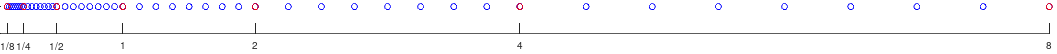
\includegraphics[scale=.4]{escala.png}
\caption{Algunos números positivos de máquina con $b=2$ y $m=4$. Notar que los números son equiespaciados únicamente entre potencias sucesivas de $2$, y que la cantidad de números de máquina en esos rangos se mantiene constante.}
\end{figure}
\begin{tcolorbox}{\bf Distribución de los números de máquina:}
Los números de máquina no se distribuyen de manera uniforme. Describamos dos números de máquina consecutivos  $x_1<x_2$ asumiendo, para simplificar,  que $0<x_1$ y que se escribe:
$$(x_1)_b= 0.b_0b_1b_2...b_{m-1}\, b^{e}.$$
Un momento de reflexión nos dice que el próximo número de máquina (salvo que haya overflow) será
$$(x_2)_b=0.b_0b_1b_2...(b_{m-1}+1)\, b^{e}$$
salvo que $b_{m-1}=b-1$ en cuyo caso
$$(x_2)_b=0.b_0b_1b_2...(b_{m-2}+1)0\, b^{e}$$
salvo que también $b_{m-2}=b-1$ en cuyo caso habrá que repetir el argumento y eventualmente -en caso de que $b_i=b-1$ para todo $0\le i\le m-1$
$$(x_2)_b=0.1b^{e+1}.$$
En cualquier caso observamos que
$$
x_2-x_1=b^{-m}b^e
$$
\emph{no es constante} al variar el exponente $e$, pero sí lo es para cada exponente fijo dado.

\end{tcolorbox}

La consecuencia mas notable de la distribución de los números de máquina es que si $x\in \R$, y existen $x_1<x_2$ números de máquina tales que $x_1\le x\le x_2$ (i.e. $x$ esta dentro de las escalas manejadas por la máquina) entonces
$$
|x-fl_{redond}(x)|\le \frac12 b^{e-m}
$$
$$
|x-fl_{trunc}(x)|\le b^{e-m}
$$
para los casos de redondeo y truncado respectivamente.
\begin{tcolorbox}{\bf Error relativo y precisión de la máquina:}
Nos concentraremos en el caso de redondeo, por lo que asumiremos de aquí en mas que  $fl=fl_{redond}$. Queremos acotar el error relativo al almacenar un número $x\neq 0$.  Observando que
$$b^{e-1}=|0.1\, b^{e}|\le  |x|,$$
resulta
$$
|\frac{x-fl(x)}{x}|\le \frac12 b^{1-m}.
$$
Notar que el error relativo depende \emph{del tamaño de la mantisa}. En el caso de base $b=2$ y $m=52$ mencionado antes resulta:
$$
|\frac{x-fl(x)}{x}|\le  2^{-52}\sim 10^{-16}.
$$
este número, propio de cada máquina, se denomina: precisión de la máquina o épsilon de la máquina y se denota con $\varepsilon$.

En el caso del ejemplo, en terminos simples, dice que nuestra máquina almacena 16 dígitos exactos (en base 10). Naturalemente sería ideal conservar esta precisión a lo largo de las  operaciones que debamos realizar a partir de  $fl(x)$. Eso, como veremos a continuación,  no es posible en general.
\end{tcolorbox}

Como acabamos de ver, en general ocurre que
$x\neq fl(x)$\footnote{Notemos que incluso números muy sencillos como $\frac{1}{10}$ no son de máquina y la introducción de un error de redondeo es inevitable. Evalúe en Python la expresión
$0.1+0.1+0.1!=0.3$, qué obtiene?.}. . Sin embargo podemos garantizar que la diferencia verifica
$$
x-fl(x)=\mu_x x,
$$
con
$$
\frac{|x-fl(x)|}{|x|} =|\mu_x|\le \varepsilon.
$$
Veamos entonces que ocurre con estos errores al efectuar alguna operación
sencilla como por ejemplo sumar. Vamos a distinguir la operación realizada por la máquina con el símbolo $\oplus$.

Pretendemos calcular $x+y$, de modo simplificado la máquina realiza las siguientes operaciones: primero
$$
x\to fl(x) \qquad y\to fl(y)
$$
luego suma $fl(x)+fl(y)$ y finalmente almacena el resultado
$$
fl(x)+fl(y)\to fl(fl(x)+fl(y)).
$$
Cómo se comportará el error resultante?.
Por una lado tenemos:
$$fl(x)=x(1+\mu_x),\qquad  fl(y)=y(1+\mu_y
y),$$ por lo que
$$fl(fl(x)+fl(y))=(fl(x)+fl(y))(1+\mu_z)$$
y en definitiva
$$
x\oplus y =fl(fl(x)+fl(y))=(x(1+\mu_x)+y(1+\mu_y
y))(1+\mu_z).
$$
Vemos entonces que \emph{si $0<x,y$} es posible acotar
$$
|x\oplus y -(x+y)|\le (x+y)2\mu +O(\varepsilon^2)
$$
con $|\mu|\le \varepsilon$. Es decir que hemos de algún modo preservado el tamaño del error relativo\footnote{Cuando los errores se acumulan de forma aditiva, como en este caso, estamos en un buen escenario porque harían falta una enorme cantidad de operaciones para deteriorar el error inicial.}  Como es  bien sabido, eso no es posible si \emph{restamos}
números similares\footnote{Verifique que la cuenta anterior no puede repetirse si los signos de $x$ e $y$ difieren.}.
Un ejemplo elemental es el siguiente: tomemos $b=10$, $m=4$, la precisión es $\varepsilon=\frac{1}{2}10^{-3}=0.0005$. Si $x=125,49$ e $y=125,31$ tenemos respectivamente
$x-y=0.18$
$x\ominus y=0.2$ por lo que el error relativo es
$$
|\frac{x-y-x\ominus y}{x-y}|=\frac{0.02}{0.18}\sim 0.11,
$$
es decir que a pesar de que $\varepsilon \sim 10^{-3}$ el error en la cuenta anterior es del $11\%$. El ejemplo anterior muestra que en una simple operación podemos perder dígitos significativos (de hecho nuestra máquina no ha acertado ningún dígito de la solución). Como regla general deben evitarse restas de números similares\footnote{Ver la guía de ejercicios para mas ejemplos} para evitar la denominada \emph{cancelación catastrófica}.

Es fácil construir ejemplos de números de máquina $0<x<y$ en los cuales no solo $x+y\neq x\oplus y$ sino que, por ejemplo, $x\oplus y=y$. En particular es fácil ver que
\begin{equation}
 \label{eq:epsilonmasuno}
 1 \oplus\varepsilon> 1,
\end{equation}
y
$$
1\oplus\varepsilon/2=1
$$
lo que da una posible definición alternativa del $\epsilon$ como el menor número de máquina con la  propiedad \eqref{eq:epsilonmasuno}.
Otras cuestión que aparece entonces en la aritmética de la máquina es la pérdida de la propiedad asociativa, ya que usando los comentarios previos vemos que por ejemplo
$$
(1\oplus \varepsilon/2)\oplus \varepsilon/2=1\neq 1\oplus (\varepsilon/2+\varepsilon/2).
$$

Hay diversas fuentes de errores computacionales que pueden estropear completamente el resultado de los algoritmos. En este sentido hay dos conceptos que nombraremos tangencialmente ya que no son objeto central de este curso: la \emph{condición} y la \emph{estabilidad}.
\section{Condición y Estabilidad}
De manera muy general, un \emph{problema bien condicionado} es aquél que reacciona benignamente con los errores en los datos. Es decir, que sus soluciones no varían demasiado al no variar demasiado los datos. Por el contrario, si un problema está muy mal condicionado, no lograremos resolverlo con mucha precisión aunque limitemos los errores en los datos (salvo que trabajemos con precisión infinita). La noción de condición es algo \emph{intrínseco del problema} y está mas allá de nuestro algoritmo de resolución.  Por otra parte, cuando los problemas están bien condicionados tenemos esperanza de resolverlos con precisión siempre que nuestro algoritmo no incremente desproporcionadamente los errores inherentes a los datos. En este caso hablaramos de \emph{algoritmos estables} y por el contrario, de  \emph{algoritmos inestables} si no cumplen con este criterio. La estabilidad entonces es algo \emph{intrínseco del algoritmo}.




\begin{tcolorbox}
Es posible dar una expresión precisa para la noción de condición, a través del llamado
\emph{número de condición}. Consideremos el problema de evaluar una función en el valor $x_0\neq 0$. Si por alguna razón (error de medición o redondeo) modificamos el dato a evaluar $x_0$ en un una cierta magnitud pequeña $h$ entonces el error relativo que cometeremos es (asumiendo que la función es de continuamente diferenciable)
$$
\frac{f(x_0+h)-f(x_0)}{f(x_0)}=
\frac{hf'(\eta)}{f(x_0)},$$
para cierto $\eta$ intermedio entre $x_0$ y $x_0+h$. Esto indica que para $h\sim 0$
$$
\frac{hf'(\eta)}{f(x_0)}\sim
\frac{x_0f'(x_0)}{f(x_0)}\frac{h}{x_0}
$$
el error relativo en los datos $\frac{h}{x_0}$ se magnifica en nuestro problema en un factor
$$
\frac{|x_0||f'(x_0)|}{|f(x_0)|},
$$
llamado el \emph{número de condición} de evaluar $f$ en $x_0$. Siguiendo un razonamiento similar vemos que para la versión $f:\Rn\to \Rm$ puede definirse el número de condición de este problema de la forma\footnote{Un ejemplo concreto y elemental de mal condicionamiento es, como hemos visto, la resta de números similares: si escribimos
$f:\R^2\to \R$, $f(x,y)=x-y$, se tiene $Df(x_0,y_0)=(1,-1)$, $\|(1,-1)\|_{\infty}=2$, $\|(x_0,y_0)\|_{\infty}=max\{|x_0|,|y_0|\}$, luego $\frac{\|x_0\|\|Df(x_0)\|}{\|f(x_0)\|}\sim \frac{1}{\|x_0-y_0\|}.$}
\end{tcolorbox}
Como ejemplo de lo anterior
si queremos evaluar $tg(x)$ en un $x_0<\pi/2$, $x_0\sim \pi/2$ vemos que el número de condición
$$
\frac{x_0}{sen(x_0)cos(x_0)},
$$
cumple que
$$
\lim_{x_0\to \pi/2^-} \frac{x_0}{sen(x_0)cos(x_0)}=+\infty.
$$
En particular si elegimos  $x_0$ tal que $\frac{x_0}{sen(x_0)cos(x_0)}\sim 10^{16}$ no esperamos tener ningún dígito significativo en nuestro cálculo de $tg(x_0)$.
%\footnote{Paul Olum, sabiendo que a su amigo Feynmann le gustaba sorprender a todos haciendo cálculos mentales, le pidió un día que aproximara mentalmente $tg(10^{100})$. Feynmann supo al instante que estaba condenado.}.


En los años 50, Wilkinson experimentaba con las primeras computadoras y rápidamente comenzó a observar fenomenos de inestabilidades y mal condicionamiento\footnote{En sus propias palabras: ``The cosy relationship that mathematics enjoyed with polynomials suffered a severe setback in the early fifities where electronic computers came into general use. Speaking for myself I regard it as the most traumatic experience in my carrer as a numerical analyst'' \cite{Wil}  }. Una cosa que notó, al probar un algoritmo de aproximación de raices, es que si al polinomio
$$
p(x)=\prod_{i=1}^{20}(x-i)
$$
se le perturba el coeficiente que acompaña a $x^{19}$ (cuyo valor es $210$ ) en $2^{-23}$ las raíces mayores a $7$ sufren considerables modificaciones. En particular las raices  $10,11,\dots 19$
se transforman en 5 pares complejos conjugados. Las $18$ y $19$ en complejos de la forma $19.5\dots\pm 19.5\dots i$, es decir que una perturbación de orden $2^{-23}$ genera variaciones de orden $1$. \footnote{A pesar de esto, se puede probar que las raíces dependen de forma continua respecto de los coeficientes.} Mostrando que el problema de calcular raices está muy mal condicionado.

Ejemplos de algoritmos inestables abundan. La inestabilidad es muy frecuente y se hace notar muy rápidamente porque los resultados obtenidos difieren notoriamente de lo esperado. Los casos mas extremos aparecen en procesos que deben iterarse en los cuales el error se acumula exponencialmente en vez de aditivamente. Sin embargo hay casos muy simples que pueden ejemplificarse.


Mas arriba vimos que restar números similares es un problema mal condicionado y por eso debe evitarse o tratarse con cautela.

Supongamos que queremos evaluar $e^{-12}$. Usando lo explicado mas arriba, podemos ver que se trata de un problema bien condicionado.  Si utilizamos un algoritmo basado en la serie convergente
$$
e^{-x}=1-x+\frac{1}{2!}x^2-\frac{1}{3!}x^3\cdots
$$
para una evaluación directa en $x=-12$ obtenemos, sumando los primeros 50 términos de la serie:
$$
e^{-12}\sim 6.144189436702122\cdot 10^{-6}.$$
Si por otro lado modificamos el algoritmo calculado primero $e^{12}$
sumando los primeros 50 terminos de la serie
$$
e^{x}=1+x+\frac{1}{2!}x^2+\frac{1}{3!}x^3\cdots
$$
y luego invirtiendo $1/e^{12}$ obtenemos
$$e^{-12}\sim 6.144212353328213\cdot 10^{-6}.$$
La pregunta es a priori, cuál de las dos respuestas es mas confiable. Sin duda el segundo método es mas estable. La razón es que en el cómputo de la serie alternada, muchos terminos ``grandes'' deben cancelarse mágicamente para producir el resultado ``pequeño'' $e^{-12}$. Los errores relativos pequeños son proporcionalmente grandes en términos del resultado final. De hecho
$$e^{-12}\sim 6.1442123533282097586823081788055323112239893148882529755...\cdot 10^{-6}$$
es decir que solo obtuvimos $4$ dígitos correctos con nuestro primero algoritmo pero $14$ con el segundo.
El segundo método es mucho mas estable que el primero. Puede probar los calculos previos con el algoritmo:

\begin{Shaded}
\begin{lstlisting}[language=python]
import numpy as np
import math 
v=np.arange(0,50)
resulI=0.0 
resulE=0.0 
for i in v:
	resulI=resulI+1/math.factorial(i)*(-12.0)**i
	resulE=resulE+1/math.factorial(i)*(12.0)**i 
resulE=1/resulE 
print(resulInes)
print(resulEs)
\end{lstlisting}
\end{Shaded}
Los problemas que emergen debido a la precisión limitada de las máquinas dan lugar a muchos comportamientos inesperados. El ejemplo que damos a continuación, debido a Cleve Moler, es particularmente sencillo y sigue las consideraciones del ejemplo previo. Queremos evaluar $p(x)=(x-1)^7$ para posteriormente graficarlo.
En el primer algoritmo usamos la expresión cerrada $(x-1)^7$  y en el segundo método la expresión equivalente
$$
p(x)=x^7-7x^6+21x^5-35x^4+35x^3-21x^2+7x-1.
$$
En la Figura \ref{fig:moler} a la izquierda vemos ambos gráficos perfectamente superpuestos (azul para el primer método tapado por el rojo del segundo método).
\begin{figure}
 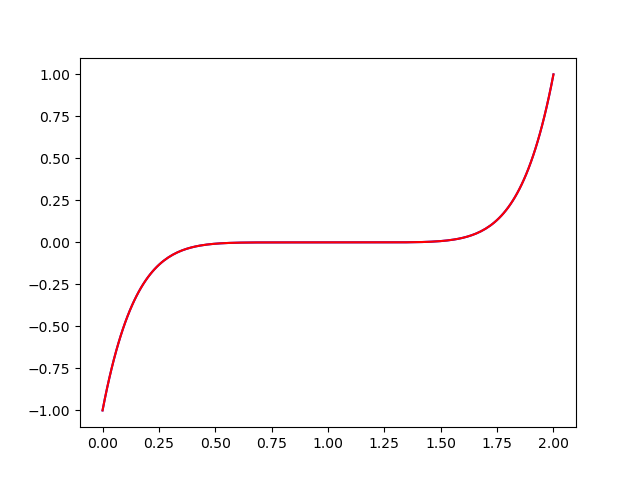
\includegraphics[scale=0.4]{moler1}
 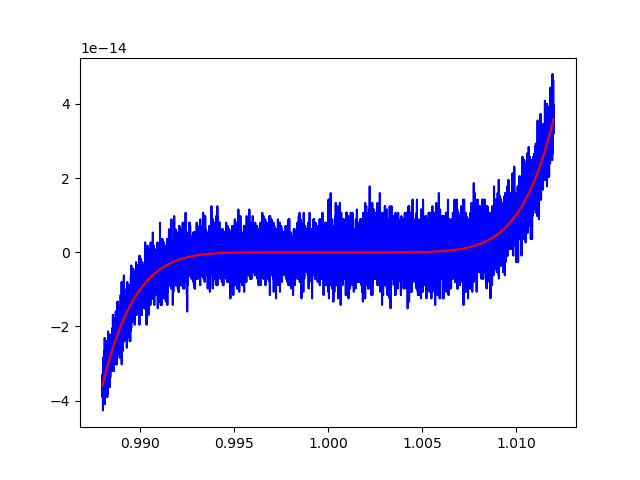
\includegraphics[scale=0.4]{moler2}
 \caption{Gráficos de $p(x)$}
 \label{fig:moler}
 \end{figure}
Sin embargo en la misma figura a la derecha se muestra un zoom cerca de la raíz del polinomio.

\begin{Shaded}
\begin{lstlisting}[language=python]
import numpy as np
import matplotlib.pyplot as plt
x=np.linspace(0,2,200)
plt.plot(x,x**7-7*x**6+21*x**5-35*x**4+35*x**3-21*x**2+7*x-1,'b', x,(x-1)**7,'r')
plt.show()

# Sin embargo a la derecha vemos el resultado de samplear en una
#escala mas fina alrededor de la raíz

x=np.linspace(0.988,1.012,10000)
plt.plot(x,x**7-7*x**6+21*x**5-35*x**4+35*x**3-21*x**2+7*x-1,'b', x,(x-1)**7,'r')
plt.show()
\end{lstlisting}
\end{Shaded}


Las nociones de condición y estabilidad que hemos comentado de modo superficial son temas transversales a toda el área del análisis  numérico. Como nos restringiremos a cuestiones de álgebra lineal solo hemos pretendido dar una idea somera de sus implicaciones generales. En el capítulo siguiente retomaremos la cuestión de la condición en el ámbito matricial.


%%ojo cambie el nomre no es ProductoInterno
\chapter{Normas y Producto Interno}
\setcounter{equation}{0}

\section{Normas en $\K^n$}

La distancia del punto $(x,y)\in \R^2$  al origen puede calcularse por el teorema de Pitágoras
$$
z = \sqrt{x^2 + y^2}.
$$
Generalizando esa fórmula a espacios de cualquier dimensión, definimos una norma vectorial:
$$
\|\vb\|_2 = \sqrt{v_1^2 + \dots + v_n^2},
$$
Esta norma suele llamarse norma-$2$ o norma euclídea. Esta norma,  a su vez, puede escribirse equivalentemente como
$$
\|\vb\|_2 = \sqrt{|v_1|^2 + \dots + |v_n|^2},
$$
lo cual nos da una expresión aplicable a los complejos.

\tccdefi
\begin{defi}
Una norma de un $K$-espacio vectorial es una función $\| \cdot \| : V \rightarrow \R_{\ge 0}$ que cumple las siguientes propiedades:
\begin{enumerate}
\item $\|a \vb\| = |a| \|\vb\|$, para $a \in \K$ y $\vb \in V$.
\item Si $\|\vb\| = 0$, entonces $\vb = 0$.
\item $\|\ub + \vb\| \le \|\ub\| + \|\vb\|$, para todo $\ub, \vb \in V$ \qquad (desigualdad triangular)
\end{enumerate}
\end{defi}
\etcc
Es fácil ver que la norma-2 cumple las primeras dos propiedades.  La tercera propiedad puede probarse usando la siguiente desigualdad clásica.

\begin{prop}[Desigualdad de Cauchy-Schwarz]
\label{prop:CS}
Dados $\ub, \vb \in \K^n$,
$$
\left|\sum_{i=1}^{n} \overline u_{i}v_{i}\right|\leq \|\ub\|_2\|\vb\|_2.
$$
\end{prop}
\begin{proof}
Asumamos primero que $\K=\R$. Consideremos el siguiente polinomio de grado 2 en la variable $x$
$$
p(x) = (u_1 x + v_1)^2 + \dots + (u_n x +v_n)^2  =\left(\sum _{i=1}^nu_{i}^{2}\right)x^{2}+2\left(\sum _{i=1}^nu_{i}v_{i}\right)x+\sum _{i=1}^nv_{i}^{2}.
$$

Como $p$ es una suma de cuadrados, $p(x) \ge 0$ para todo $x \in \R$  tiene o bien un raiz real doble o raíces complejas. Escribiendo $p(x)=ax^2 + bx + c$ vemos que debe ser entonces $b^2-4ac \le 0$. Es decir,
$$
4 \left(\sum _{i}u_{i}v_{i}\right)^{2}- 4 \left(\sum _{i}{u_{i}^{2}}\right)\left(\sum _{i}{v_{i}^{2}}\right)\leq 0,
$$
y eliminando el factor 4 y despejando, obtenemos la desigualdad buscada.

Si $\K=\C$ notamos, por la desigualdad triangular en los complejos\footnote{Si escribimos $z_1=a_1+ib_1,z_2=a_2+ib_2\in \C$, resulta
$|z_1+z_2|\le|z_1|+|z_2|$ sí y solo sí
$$(a_1+a_2)^2+(b_1+b_2)^2\le \left(\sqrt{a_1^2+b_1^2}+\sqrt{a_2^2+b_2^2}\right)^2,$$ desarrollar el cuadrado y ver que eso ocurre sí y solo sí $0\le(a_1b_2-a_2b_1)^2$ que obviamente siempre es válido.}


$$
\left|\sum _{i}u_{i}\overline{v_{i}}\right|\le \sum _{i}|u_{i}||\overline{v_{i}}|=\sum _{i}|u_{i}||{v_{i}}|,
$$
y la desigualdad sale ahora usando el caso real con los vectores $(|u_1|,\cdots,|u_n|)$,$(|v_1|,\cdots,|v_n|)$.
\end{proof}
\begin{rem}
Notar que la desigualdad de Cauchy-Schwarz vale también tomando a la izquierda
$\sum _{i}\overline{u_{i}}{v_{i}}$, puesto que $\sum _{i}\overline{u_{i}}{v_{i}}=\overline{\sum _{i}u_{i}\overline{v_{i}}}$ y el módulo de un complejo es igual al de su conjugado.
\end{rem}
\begin{cor}
 Para todo $\ub,\vb\in \K^n$ vale,
 $\|\ub+\vb\|_2\le\|\ub\|_2+\|\vb\|_2.$
\end{cor}
\begin{proof}
La hacemos en $\C$ y en $\R$  sale como caso particular.
$$
\|\ub+\vb\|_2^2=
\sum_{i=1}^n |u_i+v_i|^2=\sum_{i=1}^n (u_i+v_i)\overline{(u_i+v_i)}
$$
$$
=\sum_{i=1}^n u_i\overline{u_i}+
\sum_{i=1}^n(u_i\overline{v_i}+v_i\overline{u_i})+\sum_{i=1}^n v_i\overline{v_i}=\|\ub\|_2^2+\sum_{i=1}^n(u_i\overline{v_i}+v_i\overline{u_i})+\|\vb\|^2_2,
$$
los términos entre paréntesis son reales (un número complejo -eventualmente complejo- mas su conjugado), luego
$$
\sum_{i=1}^n(u_i\overline{v_i}+v_i\overline{u_i})\le
\left|\sum_{i=1}^n(u_i\overline{v_i}+v_i\overline{u_i})\right|\le\left|\sum_{i=1}^nu_i\overline{v_i}\right|+\left|\sum_{i=1}^nv_i\overline{u_i}\right| \le 2\|\ub\|_2\|\vb\|_2,
$$
donde hemos usado Cauchy-Schwarz en la última desigualdad.
Luego, se tiene
$$
\|\ub+\vb\|_2^2\le \|\ub\|^2+\|\vb\|^2+2\|\ub\|_2\|\vb\|_2=
\left(\|\ub\|_2+\|\vb\|_2\right)^2,
$$
lo que termina la demostración tomando raíz cuadrada \end{proof}
\tccdefi
Como generalización de la norma$-2$, están las normas$-p$, definidas también en  $\K^{n}$:

\begin{itemize}
\item Norma$-1$: $\| \vb \|_1 = |v_1| + \dots + |v_n|$
\item Norma-infinito: $\| \vb \|_\infty = \max\{|v_1|, \dots, |v_n|\}$
\item Norma$-p$: $\| \vb \|_p = \left(|v_1|^p  + \dots + |v_n|^p \right)^{1/p}$
\end{itemize}
\etcc

En el siguiente gr\'afico podemos ver la diferencia entre las 3 normas m\'as usuales en $\R^2$. En cada gr\'afico est\'an representados todos los puntos con norma igual a 1 bajo la norma respectiva.
\clearpage
\begin{figure}
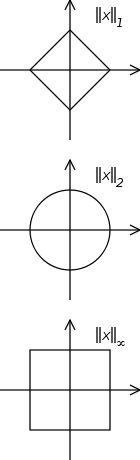
\includegraphics[scale=.3]{140px-Vector_norms.png}
\caption{``Círculos''  de radio 1 en diferentes normas. Es decir $\vb\in \R^2$ tales que $\|\vb\|=1$.}
\end{figure}
En la siguiente figura observamos distintas curvas de nivel\footnote{Las curvas en las cuales la norma respectiva permanece constante.} para distintas normas.
\begin{ej}
 Examinando los gráficos de las curvas de
nivel de las normas$-p$ se puede intuir que  $\lim_{p\to +\infty}\|\vb\|_p=\|\vb\|_\infty$. De una demostración de este hecho.
\end{ej}
\begin{figure}
 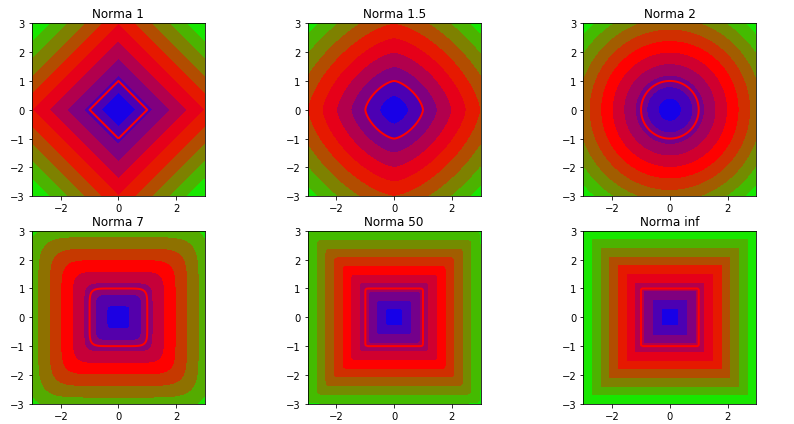
\includegraphics[scale=.4]{nivelNormas.png}
\caption{Curvas de nivel de diferentes normas$-p$.}
\end{figure}
% \begin{aplicacion}
% Para entender la diferencia entre las distintas normas, analizamos el siguiente ejercicio: Hallar gr\'aficamente el punto del plano de norma igual a 1 que maximiza la funci\'on $f(x,y) = 2y + x$. Para resolverlo, graficamos en el plano todos los puntos para los cuales $f$ tiene un valor fijo. Por ejemplo, los puntos para los cuales $f(x,y) = 3$ se encuentran en una recta que pasa por el punto $(3,0)$ y tiene pendiente $-1/2$. Si aumentamos o disminuimos este valor fijo, obtendremos una recta paralela a la anterior desplazada hacia la derecha o izquierda respectivamente.
%
% Por lo tanto, para resolver el problema, desplazamos la recta que trazamos hacia la izquierda hasta que toque a alguno de los puntos de norma 1.
% Concluimos que en el caso de la norma-1 este punto es el punto $(1,0)$, para la norma infinito este punto es el punto $(1,1)$ y para la norma 2, este punto es un punto en el arco del primer cuadrante.
%
% En general, al maximizar o minimizar la norma-1 de una función, obtendremos puntos con varias coordenadas nulas, mientras que al minimazar la norma-2 encontraremos puntos con coordenadas no nulas de valor menor que las de la norma-1. Dependiendo la aplicación resultará m\'as \'util una u otra de las normas.
% \end{aplicacion}
Para nosotros va a ser relevante medir \emph{errores} en espacios vectoriales, para ello recordemos que dados $\ub,\vb\in \R^n$
$\|\ub-\vb\|_2$ da la distancia entre ellos. En ocasiones, sin embargo, vamos a notar que es mas sencillo trabajar con una norma diferente a la norma-$2$, por lo que resulta natural ver que relación hay entre las diferentes normas-$p$. Puede probarse muy fácilmente lo siguiente.
\begin{ej}
Verificar que para todo $\xb\in \K^n$
\begin{enumerate}
\item $\|\xb\|_2 \le \|\xb\|_1 \le \sqrt{n} \|\xb\|_2$
\item $\|\xb\|_\infty \le \|\xb\|_2 \le \sqrt{n} \|\xb\|_\infty$
\item $\|\xb\|_\infty \le \|\xb\|_1 \le n \|\xb\|_\infty$
\end{enumerate}
\end{ej}
Ese resultado es un caso particular de uno mucho mas general. Primero definamos \emph{equivalencia de normas}.
\tccdefi
\begin{defi}
 Sean $\|\cdot\|$ y $\|\cdot\|_{*}$ dos normas en un $\K$-espacio vectorial $V$. Decimos que son equivalentes si existen dos constantes $0<c,C$ tales que para todo $\xb\in V$
 $$
 c\|\xb\|_* \le \|\xb\| \le C \|\xb\|_*
 $$
\end{defi}
\etcc
Vale lo siguiente,
\begin{prop}
\label{prop:equivnorm}
 En un $\K$-espacio vectorial de dimensión finita todas la normas son equivalentes\footnote{Las constantes que relacionan las normas dependen de la dimensión $n$, típicamente se deterioran si $n\to \infty$}.
\end{prop}
Este resultado nos es útil en muchos contextos.  Veamos primero la siguiente definición.
\tccdefi
\begin{defi}
Decimos que una sucesi\'on de vectores $\{v_n\}_{n \in \N}$ converge bajo una norma $\|\cdot\|$ a un vector $v$ si
$$
\|v_n - v\| \rightarrow 0 \quad \text{ cuando } n \rightarrow \infty.
$$
\end{defi}
\etcc
Como consecuencia de la Proposición \ref{prop:equivnorm}, la convergencia en una norma cualquiera implica la convergencia en todas las normas.

\section{Producto Interno}
\tccdefi
\begin{defi}
Dados dos vectores $\ub, \vb \in \K^n$ definimos\footnote{Recordemos que asociamos los vectores con las matrices columna.} el producto interno (canónico) por la fórmula\footnote{En muchos casos se suele conjugar los coeficientes del $\vb$ en la sumatoria en vez de los de $\ub$  en la definición de $\langle \ub,\vb\rangle$. Para nuestros intereses no cambia en absoluto la definición utilizada que por lo demas coinciden sobre $\R$.} $$
\langle \ub, \vb \rangle = \ub^*\vb\in \K,
$$
es decir
$$
\langle \ub, \vb \rangle=\overline{u_1} v_1 + \overline{u_2} v_2 + \dots + \overline{u_n} v_n = \sum_{i=1}^{n} \overline{u_i}v_i.
$$
\end{defi}
\etcc
Tenemos las siguientes propiedades inmediatas.

\tcc
\begin{rem}
\label{obs:interno}
Notar que para $\xb,\yb,\zb \in \K^n$, $\wb\in \K^m$ $a,b \in \K$,  $\Ab\in \K^{n \times m}$, resulta

\begin{enumerate}
\item   $\langle \xb, \yb \rangle= \overline{\langle \yb, \xb \rangle}$,
\item   $\langle \xb, a\yb + b\zb \rangle = a \langle \xb, \yb \rangle + b \langle \xb, \zb \rangle$,  y $\langle a\yb + b\zb,\xb \rangle = \overline{a} \langle \yb, \xb \rangle + \overline{b} \langle \zb, \xb \rangle$.
\item  $\langle \Ab\wb, \xb \rangle = \langle  \wb,\Ab^* \xb \rangle$\footnote{Puesto que $\langle \Ab\wb, \xb \rangle = (\Ab\wb)^*\xb=\wb^*\Ab^*\xb= \langle  \wb,\Ab^* \xb \rangle$.}
  \item $\langle a\xb, a\yb \rangle = \overline{a}a \langle \xb, \yb \rangle=|a|^2 \langle \xb, \yb \rangle$.
\item  Utilizando el producto interno, la norma-$2$ de un vector se puede definir por la fórmula $\|\vb\| = \sqrt{\langle \vb, \vb\rangle}$.
\item La desigualdad de Cauchy-Schwarz se escribe
$|\langle \vb,\wb\rangle|\le \|\vb\|_2\|\wb\|_2,$
 \end{enumerate}
\end{rem}
\etcc

\begin{ejemplo}
$\langle \xb + \yb, \xb + \yb\rangle = \langle \xb, \xb + \yb\rangle + \langle \yb, \xb + \yb\rangle = \langle \xb, \xb \rangle + \langle \xb, \yb \rangle + \langle \yb, \xb \rangle + \langle \yb, \yb\rangle = \|\xb\|^2 + 2\langle \xb, \yb \rangle + \|\yb\|^2$
\end{ejemplo}
Sean $\xb,\yb\in \R^2$, $\xb\neq \cero\neq \yb$, $\xb=(a_1,a_2)$, $\yb=(b_1,b_2)$.   Podemos escribir $\xb=\|\xb\|\frac{\xb}{\|\xb\|}$ y como $ \frac{\xb}{\|\xb\|}$ está en el círculo de radio $1$ vemos que existe un único $\alpha$, $0\le \alpha<2\pi$ tal que
$ \frac{\xb}{\|\xb\|}=(\cos(\alpha),\sen(\alpha))$. Es decir, $\xb=\|\xb\|_2(\cos(\alpha),\sen(\alpha))$. Análogamente, podemos escribir $\yb=\|\yb\|_2(\cos(\beta),\sin(\beta))$ y en particular\footnote{Recordar: $
cos(\alpha +\beta)=cos(\alpha)cos(\beta)-sen(\alpha)sen(\beta),
$
$
sen(\alpha +\beta)=sen(\alpha)cos(\beta)+cos(\alpha)sen(\beta).
$
}
$$
\langle \xb,\yb\rangle= \|\xb\|_2\|\yb\|_2\left(\cos(\alpha)\cos(\beta)+\sen(\alpha)\sen(\beta)\right)=\|\vb\|_2\|\wb\|_2\cos(\alpha-\beta),
$$
lo que dice que puede escribirse
\begin{equation}
 \label{eq:calculodeAng}
\cos(\theta)=\frac{\langle \xb,\yb\rangle}{\|\vb\|_2\|\wb\|_2},
\end{equation}
con $\theta$ el ángulo\footnote{Considerando que $\cos(\mu)=\cos(2\pi-\mu)$ siempre puede elegirse $0\le \theta < \pi$.} entre $\xb$ y $\yb$.
\begin{center}
 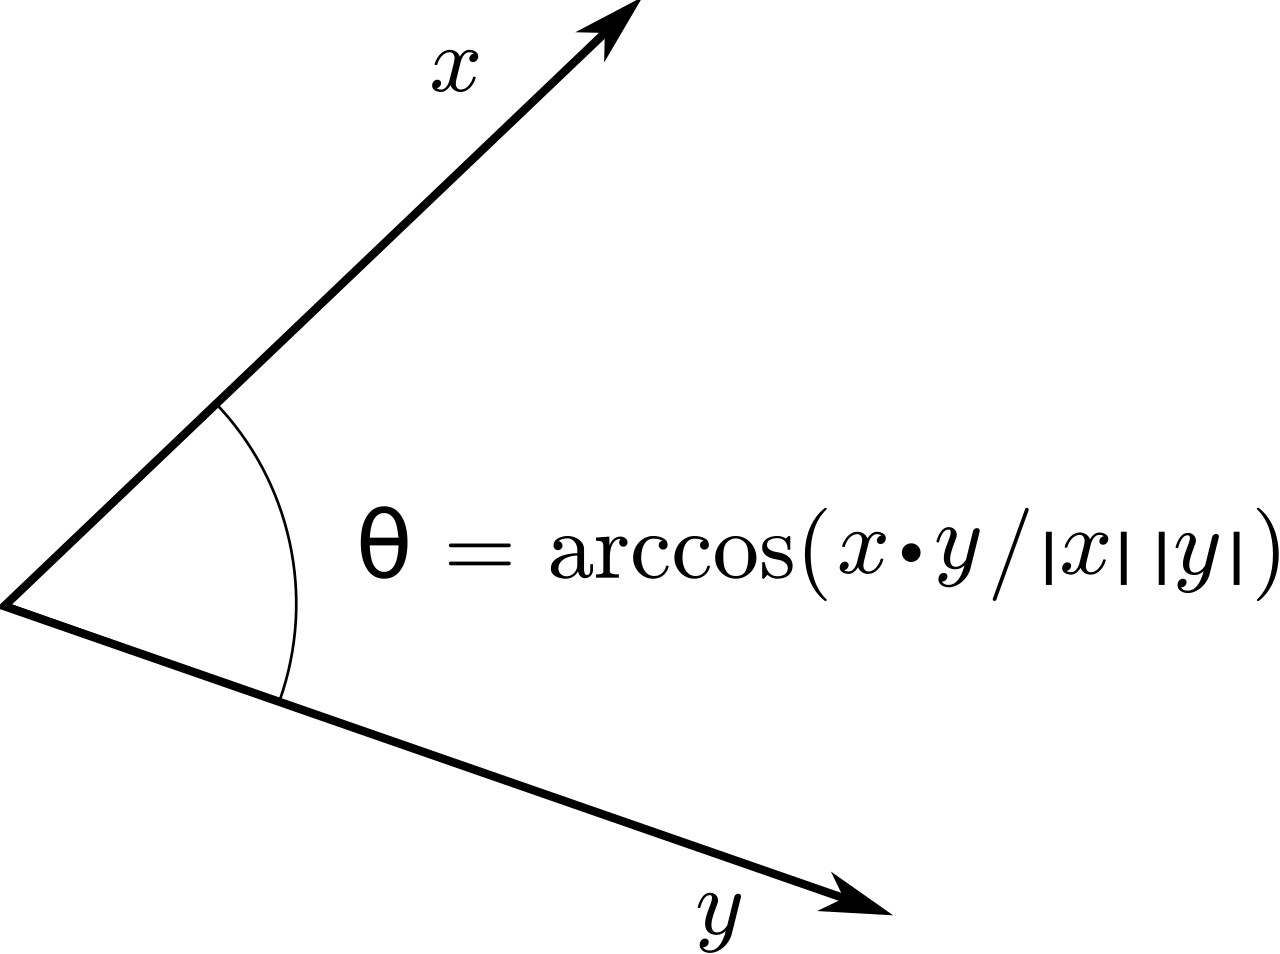
\includegraphics[scale=0.1]{angulo.png}
\end{center}
En $\Rn$ ocurre lo mismo. Ya que $-1\le\frac{\langle \xb, \yb\rangle}{\|\xb\|\|\yb\|}\le 1$, (ver (6) de la Observación \ref{obs:interno}) se define el ángulo $\theta$ entre $\xb$ e $\yb$ a través de \eqref{eq:calculodeAng}.



\tcc
Las normas nos han permitido incorporar al \emph{álgebra} (el espacio vectorial) el concepto de distancia, que  nos permitirá introducir la noción de convergencia y una forma de medir errores.  El producto escalar, por su parte, nos permite trabajar con ángulos. En particular con la idea de perpendicularidad u ortogonalidad que resulta  fundamental en el desarrollo de algoritmos estables.
\etcc
De \eqref{eq:calculodeAng} vemos que $\theta=\pi/2$ si y solo si $\vb^*\wb=0$, de ahí la siguiente definición que la extendemos a los complejos.
\tccdefi
\begin{defi}
 Dados $\vb,\wb\in\K^n$, no nulos. Decimos que son ortogonales sí y solo sí  $\vb^*\wb=\langle \vb,\wb\rangle=0.$ En este caso también usaremos la notación $\vb\perp \wb$.
\end{defi}
\etcc
\tccdefi
\begin{defi}
 Una colección de vectores  $\{\vb_i\}_{1\le i\le k}\subset \K^{n}$ se dice \emph{ortogonal} si $\langle \vb_i,\vb_j\rangle =\delta_i^j$. Si además $\|\vb_i\|_2=1$ para todo $1\le i\le k$ decimos que el conjunto es \emph{ortonormal.}
\end{defi}
\etcc
Los conjuntos ortogonales tienen muchas propiedades que pueden explotarse, tanto teóricamente como en la práctica.

Veamos una de ellas de importancia fundamental. Sea $\mathcal{B}=\{\vb\}_{1\le i\le n}\subset \K^n$ una \emph{base} ortonormal de $\K^n$. Dado $\wb\in \K^n$ queremos conocer las coordenadas de $\wb$ en la base $\mathcal{B}$. Esto se reduce a hallar los  $\{\alpha_i\}_{1\le i\le n}\subset \K$ tales que
\begin{equation}
\label{eq:escritura_ort}
\wb=\sum_{i=1}^n\alpha_i\vb_i,
\end{equation}
que como sabemos implica resolver un sistema de $n\times n$. Sin embargo en este caso particular, vemos que para cada $1\le j\le n$ el producto escalar
\begin{equation}
\label{eq:proyecciones}
\vb_j^*\wb=\sum_{i=1}^n\alpha_i\vb_j^*\vb_i=\alpha_j,
\end{equation}
permite ``despejar'' $\alpha_i$ por el módico costo de un producto escalar\footnote{Esto es $2n-1$ operaciones, $n$ productos y $n-1$ sumas.}
Desde el punto de vista matricial, sea $\Qb\in \K^{n\times n}$, que tiene por columnas los $\vb_i$. Resulta que el problema anterior se puede escribir de modo matricial
$$
\wb=\Qb\begin{pmatrix}
        \alpha_1\\
        \vdots\\
        \alpha_n
       \end{pmatrix},
$$
y de la expresión de mas arriba vemos que
$$
\Qb^*\wb=\begin{pmatrix}
        \alpha_1\\
        \vdots\\
        \alpha_n
       \end{pmatrix}.
$$
Esto no expresa mas que el hecho de que invertir $\Qb$ se reduce a conjugar (trasponer si $\K=\R$) lo que a su vez es inmediato considerando que sus columnas son ortonomales\footnote{El costo total de resolver el sistema es $n(2n-1)\sim O(2n^2)$ operaciones. } y así
$$
[\Qb^*\Qb]_{ij}=\vb_i^*\vb_j=\delta_i^j.
$$
Estas matrices tienen un nombre particular.
\begin{defi}
\label{def:de_unitaria}
 Una matriz $\Qb\in \K^{n\times n}$ se dice \emph{unitaria} (suele llamarse \emph{ortogonal} cuando $\K=\R$) si
 $\Qb^*\Qb=\Ib$ ($\Qb^T\Qb=\Ib$ si $\K=\R$).
\end{defi}
\begin{rem}
$\Qb$ es unitaria (resp. ortogonal) si y solo si $\Qb^*$ es unitaria (resp. ortogonal).
\end{rem}
Estudiemos ahora el problema de calcular la proyección \emph{ortogonal} de un vector $\wb$ sobre la recta generada por otro vector $\vb\neq \cero$ (ver Figura \ref{fig:proyusobrev}).
Es decir, que buscamos un vector $\beta\vb$
 tal que $(\beta\vb -\wb)\perp \vb$, esto equivale a
 $(\beta\vb -\wb)^* \vb=0$, lo que indica que $\overline{\beta}=\frac{\wb^*\vb}{\|\vb\|_2^2}$, es decir
 $$
 \beta=\frac{\vb^*\wb}{\|\vb\|_2^2}.
 $$
 Si $\|\vb\|=1$ la expresión coincide con la de los $\alpha$ calculados en \eqref{eq:proyecciones}, lo que nos da una interpretación alternativa de \eqref{eq:escritura_ort}. Esto es, llamando
 $\Pb_{\vb}(\wb)$ a la proyección ortogonal de $\wb$ sobre el subespacio generado por $\vb$, vemos que
\begin{equation}
 \label{eq:proy_forma1}
 \Pb_{\vb}(\wb)=\frac{\vb^*\wb}{\|\vb\|_2^2}\vb,
\end{equation}
y en particular \eqref{eq:escritura_ort} toma la forma
 $$
 \wb=\sum_{1\le i\le n}\Pb_{\vb_i}(\wb).
 $$

\begin{figure}
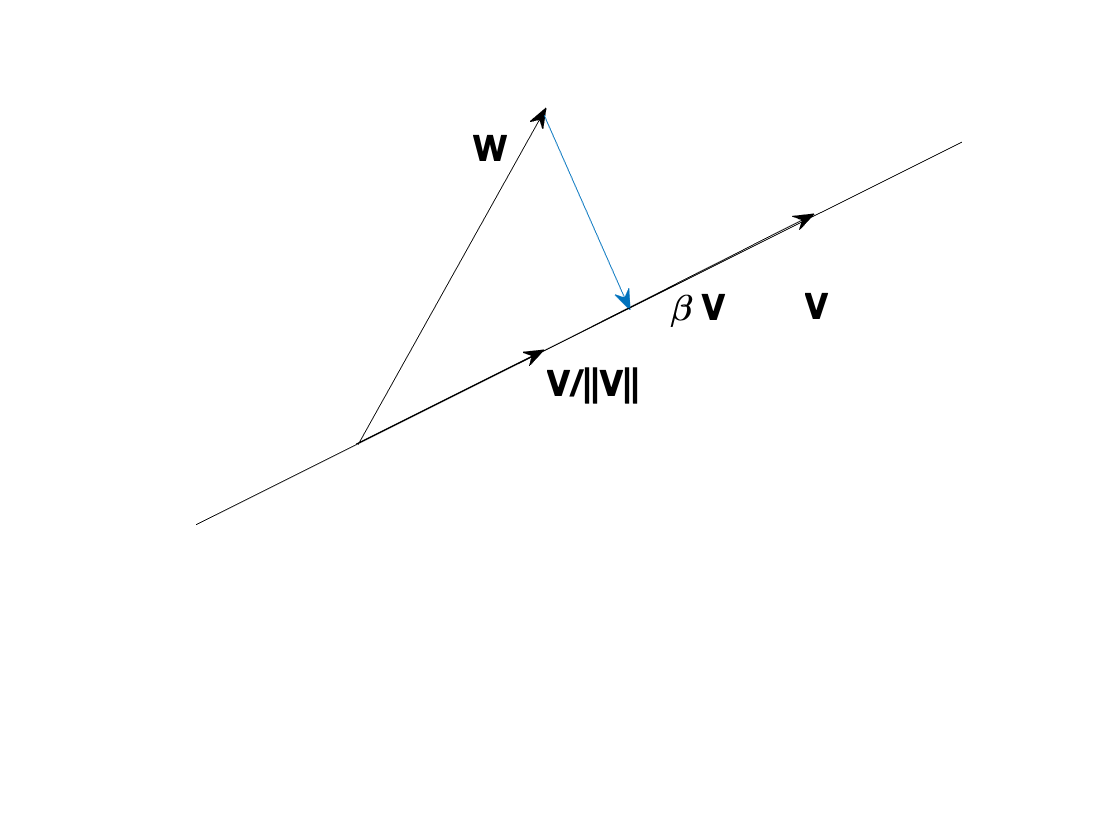
\includegraphics[scale=0.15]{proywsobrev.png}
\caption{Proyección de $\wb$ sobre la recta generada por $\vb$.}
 \label{fig:proyusobrev}
\end{figure}

\tcc
De los argumentos previos vemos que \emph{en una base ortonormal}, las proyecciones ortogonales de un vector $\wb$ sobre los elementos de la base nos dan sus coordenadas en esa base. Eso  es justamente a lo que estamos acostumbrados en la base can\'onica.
\etcc
Otro hecho de gran importancia es la generalización del teorema de Pitágoras en cualquier dimensión si tenemos una base ortonormal. Esto es, de la expresión \eqref{eq:escritura_ort}, tenemos que el cuadrado de la longitud de $\wb$ (el cuadrado de la ``hipotenusa'') es, por un lado
$$\|\wb\|^2_2=\wb^*\wb$$ y por el otro
$$
(\sum_{i=1}^n\alpha_i\vb_i)^*(\sum_{i=1}^n\alpha_i\vb_i)=(\sum_{i=1}^n\overline{\alpha_i}\vb_i^*)(\sum_{i=1}^n\alpha_i\vb_i)=
\sum_{i,j=1}^n\overline{\alpha_j}\alpha_i\vb_j^*\vb_i=\sum_{i=1}^n\overline{\alpha_i}\alpha_i=\sum_{i=1}^n|\alpha_i|^2,
$$
es decir el cuadrado de la suma de las longitudes de las coordenadas (los ``catetos'').
Para resaltar este hecho que usaremos en lo sucesivo, lo recuadramos,
\tcc
\begin{rem}
\label{obs:pitagoras}
En toda base ortonormal $\mathcal{B}=\{\vb_1,\cdots,\vb_n\}$, si
$$
\wb=\sum_{i=1}^n\alpha_i\vb_i,
$$
entonces
$$
\|\wb\|^2=\sum_{i=1}^n|\alpha_i|^2.
$$
\end{rem}
\etcc
Mas adelante volveremos sobre el tema de las proyecciones.

Para finalizar la sección de producto interno definimos

\tccdefi \begin{defi}
 Una matriz $\Ab\in \Cnn$ se dice \emph{Hermitiana} si $\Ab=\Ab^*$. En el caso de que $\Ab\in \Rnn$, $\Ab$ se dice \emph{simétrica}.
\end{defi}
\etcc
Si $\Ab\in \Knn$ es Hermitiana, entonces, para todo $\vb\in \Kn$, $\vb^*\Ab\vb\in \R$. En efecto, por un lado, debido a las dimensiones de los elementos que aparecen en el producto, se tiene  $z=\vb^*\Ab\vb\in \K$, por otro lado puesto que
$$\overline{\vb^*\Ab\vb}=(\vb^*\Ab\vb)^*=\vb^*\Ab^*(\vb^*)^*=\vb^*\Ab\vb,$$
resulta de la primera y ultima expresión de la cadena de igualdades que $\overline{z}=z$, es decir $z\in \R$.

\tccdefi
\begin{defi}
\label{def:positiva}
 Una matriz $\Ab\in \Cnn$ ($\Ab\in \Rnn$)  se dice \emph{definida positiva} si es Hermitiana (simétrica) y además $\vb^*\Ab\vb>0$ para todo $\vb\neq 0$.  Si por otro lado $\vb^*\Ab\vb\ge0$ para todo $\vb$, la matriz se dice \emph{semi definida} positiva.
\end{defi}
\end{tcolorbox}


\section{Normas de matrices}
Dada una matriz $A \in \K^{n \times m}$, se la puede pensar pensar como un vector de $\K^{nm}$ y en consecuencia se aplicaría a las matrices todo lo que hemos desarrollado para normas vectoriales.  Sin embargo, salvo casos excepcionales\footnote{Como la norma de Frobenius que veremos mas adelante.}, esta normas no son de gran utilidad en el contexto de las matrices. Esto es debido a que nos interesa estudiarlas desde la perspectiva  de las trasformaciones lineales asociadas. Por esta razón se introducen las normas subordinadas.

Dada una matriz $\Ab \in \K^{n \times m}$, y un par de normas vectoriales $\|\cdot\|_n,\|\cdot\|_m$ en $\K^n$ y $\K^m$ respectivamente, definimos
$$
\|\Ab\|_{n,m} = \max_{\cero \neq \xb \in \K^m} \frac{\|\Ab\xb\|_n}{\|\xb\|_m} = \max_{\xb \in \K^m, \|\xb\|_m = 1} \|\Ab\xb\|_n.
$$
Un caso usual en este curso es que la matriz sea cuadrada $\Ab \in \K^{n \times m}$ y en ese caso usamos una sola norma vectorial $\|\cdot\|$
\tccdefi
\begin{equation}
 \label{eq:defidenormaA}
\|\Ab\| = \max_{\cero \neq \xb \in \K^m} \frac{\|\Ab\xb\|}{\|\xb\|} = \max_{\xb \in \K^m, \|\xb\| = 1} \|\Ab\xb\|.
\end{equation}
\etcc

Estas normas matriciales se dicen \emph{subordinadas} a la norma vectorial $\|\cdot\|$ que estamos utilizando
en el espacio $\Kn$ . De su definición vemos que  la norma (subordinada) de una matriz mide en qué proporción puede aumentar como máximo la norma de un vector $\xb$ al multiplicarlo por $\Ab$.

\begin{ej}
Sea $\Ab\in \Knn$ y $\|\cdot\|$ una norma en $\Kn$, entonces
 \eqref{eq:defidenormaA} define una norma.
\end{ej}
\begin{ej}
\label{ej:idnorma1}
Sea $\Ib\in \Knn$ la identidad, entonces
 $\|\Ib\|=1$ para toda norma subordinada (siempre que pensemos $\Kn$ con la misma norma vectorial como espacio de partida y llegada de la transformación $\Ib:\Kn\to \Kn$).
\end{ej}

También resulta inmediato de la definición que para todo $\xb$
\begin{equation}
 \label{eq:acotacionoperador}
\|\Ab\xb\|\le \|\Ab\|\|\xb\|.
\end{equation}
De aquí se obtiene la siguiente propiedad. Para todo par de matrices\footnote{Como se desprende de la cuenta,  también vale para matrices rectangulares, siempre que pueda hacerse el producto $\Ab\Bb$.} $\Ab, \Bb\in \Knn$, y toda \emph{norma subordinada}
\begin{equation}
 \label{eq:prodnormas}
\|\Ab\Bb\|\le \|\Ab\|\|\Bb\|.
\end{equation}
En efecto,
dos aplicaciones sucesivas de \eqref{eq:acotacionoperador} da
$$
 \|\Ab\Bb\|=\max_{\|\xb\|=1}
\|\Ab\Bb\xb\|\le \max_{\|\xb\|=1}
\|\Ab\|\|\Bb\xb\|\le \max_{\|\xb\|=1}\|\Ab\|\|\Bb\|\|\xb\|=\|\Ab\|\|\Bb\|,$$
que prueba \eqref{eq:prodnormas}.
Aplicando sucesivamente \eqref{eq:prodnormas}, vemos que para toda matriz cuadrada y para todo $k\in\N$, vale\footnote{Que ocurre si $k\in \mathbb{Z}$ con $k<0$?. Por ejemplo, cuando $\Ab$ es invertible sabemos darle sentido a $\Ab^{-1}$ como la inversa de $\Ab$.
Por lo tanto $\Ib=\Ab\Ab^{-1}$ de donde $1\le \|\Ab\|\|\Ab^{-1}\|$  (hemos usado aquí el Ejercicio \ref{ej:idnorma1}) y de ahí $\|\Ab\|^{-1}\le \|\Ab^{-1}\|$. Es decir al revés que en  \eqref{eq:normasypotencias}.  Piense que ocurre en general. Defina primero $\Ab^{k}$ con $k<0$. Como ayuda pregúntese que será por ejemplo $\Ab^{-3}$?. Vea que puede pensarlo como $\Ab^{-3}:=\left(\Ab^{-1}\right)^3$, es decir $\Ab^{-3}=\Ab^{-1}\Ab^{-1}\Ab^{-1}$. Pero otro lado $\Ab^3\left(\Ab^{-1}\Ab^{-1}\Ab^{-1}\right)=\Ib$, lo que dice que la primera definición coincide con $(\Ab^3)^{-1}$. Use estas consideraciones para responder la pregunta.}
\begin{equation}
 \label{eq:normasypotencias}
\|\Ab^k\|\le \|\Ab\|^k.
 \end{equation}
En algunos pocos casos es posible calcular explícitamente la expresión de $\|\Ab\|$.

\begin{ejemplo}
Consideremos en $\K^n$ la norma $\|\cdot\|_\infty$. Para $\Ab\in \Knn$ se tiene\footnote{También vale la demostración en el caso de matrices rectangulares.}
\tcc
$$
 \|\Ab\|_\infty=\max_{1\le i\le n}\{\sum_{j=1}^{n} |a_{ij}|\}.
$$
\etcc
\begin{proof}
 Lo vemos para $\K=\R$. Debemos calcular
$$\|\Ab\|_\infty =
\max_{\xb \in \R^n, \|\xb\|_\infty = 1} \|\Ab\xb\|_\infty.
 $$
 Llamemos $k$ a la fila donde ser realiza el máximo, es decir
 $$
 \max_{1\le i\le n}\{\sum_{j=1}^{n} |a_{ij}|\}=\sum_{j=1}^{n} |a_{kj}|,
 $$
 (si hay más de una tomamos cualquiera). Podemos suponer que
 $\sum_{j=1}^{n} |a_{kj}|>0$ de otro modo el resultado es inmediato. Llamemos $\zb$ al vector de los signos de los elementos de esa fila $\zb=(sg(a_{k,1}),\cdots ,sg(a_{k,n})$. Si algún $a_{k,i}=0$ tomamos $sg(a_{k,1})=0$. Como la fila no es nula, $\zb\neq\cero$. Luego $\|\zb\|_\infty=\max_{1\le i\le n}\{|z_i|\}=1$, y  haciendo
 $$
\|\Ab\|_\infty =\max_{\xb \in \R^n, \|\xb\|_\infty = 1} \|\Ab\xb\|_\infty
 \ge \|\Ab\zb\|_\infty\ge \sum_{j=1}^n a_{i,j}sg(a_{i,j})=\sum_{j=1}^n |a_{i,j}|=\max_{1\le i\le n}\{\sum_{j=1}^{n} |a_{ij}|\},
 $$
 lo que prueba una desigualdad. Para a otra desigualdad, sea $\xb\in \R^n$ tal que $\|\xb\|_\infty=1$, luego para todo $1\le j\le n$ $|x_j|\le \|\xb\|_\infty=1$ y entonces, para cualquier elemento $i$ del vector $\Ab\xb$
$$
|[\Ab\xb]_i|=|\sum_{j=1}^na_{i,j}x_j |\le \sum_{j=1}^n|a_{i,j}|\le \max_{1\le i\le n}\{\sum_{j=1}^{n} |a_{ij}|\},
$$
lo que da la otra desigualdad y demuestra el caso $\K=\R$.
El caso $\K=\C$ sale del mismo modo recordando que si $z\in \C$ y $z=|z|e^{i\theta}$, se tiene que $ze^{-i\theta}=|z|$ y $|e^{i\theta}|=1$.
\end{proof}
Análogamente para la norma$-1$ se tiene
\end{ejemplo}

\begin{ejemplo}
Consideremos en $\K^n$ la norma $\|\cdot\|_1$. Para $\Ab\in \Knn$ se tiene\footnote{También vale  en el caso de matrices rectangulares.}
\tcc
$$
 \|\Ab\|_1=\max_{1\le j\le n}\{\sum_{i=1}^{n} |a_{ij}|\}.
$$
\etcc
\end{ejemplo}
Un caso de mucha importancia para nosotros es la norma matricial subordinada a la norma$-2$.
Comencemos calculando un caso elemental: la norma$-2$ de una matriz unitaria/ortogonal (Definición \ref{def:de_unitaria}).
Supongamos que $\Qb\in \Knn$ y $\Qb^*\Qb=\Ib$, luego, para todo$\xb\in\Kn$
$$
\|\Qb\xb\|_2^2=(\Qb\xb)^*\Qb\xb=\xb^*\xb=\|\xb\|^2_2,
$$
es decir que
\begin{equation}
\label{eq:isometria}
\|\Qb\xb\|_2=\|\xb\|_2, \, \forall \xb\in \K^n.
\end{equation}
 Vemos que las matrices unitarias son \emph{isometrías}, es decir, no cambian las longitudes. Tampoco cambian los ángulos ya que preservan el producto interno, propiedad que resaltamos a continuación 
 \tcc
 \begin{equation}
 \label{eq:preservaPI}
\langle \Qb\vb,\Qb\wb \rangle=(\Qb\vb)^*\Qb\wb=\vb^*\wb=\langle \vb,\wb \rangle.
 \end{equation}
\etcc
Estas propiedades definen a los \emph{movimientos rígidos}. De \eqref{eq:isometria}, tenemos
$$
\|\Qb\|_2=\sup_{\xb\neq\cero}\frac{\|\Qb\xb\|_2}{\|\xb\|_2}=1,
$$
lo que les da su nombre a las matrices unitarias.
\begin{ej}Verificar que la matriz
$$
\Ab = \begin{pmatrix}
1 & 0 & 0 \\ 0 & \cos \alpha & -\sin \alpha \\ 0 & \sin \alpha & \cos \alpha
\end{pmatrix}
$$
es una matriz ortogonal para cualquier valor de $\alpha$. Interpretar geométricamente la transformación lineal $\Ab\xb$.
\end{ej}

Como ya hemos señalado, las normas subordinadas son las mas útiles. Sin embargo la norma euclídea aplicada a matrices -que es no subordinada- tiene importantes aplicaciones y un nombre propio.
\tccdefi
\begin{defi}
 Dada $\Ab\in \K^{n\times m}$ definimos la norma de Frobenius
 $$
 \|\Ab\|_F=\sqrt{\sum_{1\le i\le n}\sum_{i\le j\le m} |a_{i,j}|^2}
 $$
\end{defi}
\etcc
Notar que
$$
\|\Ab\|_F=\sqrt{tr(\Ab^T\Ab)},
$$
donde $tr$ indica el operador traza (la suma de los elementos de la diagonal). Las normas no subordinadas de matrices no suelen cumplir con la desigualdad \eqref{eq:prodnormas}. La norma de Frobenius es una excepción, gracias a la desigualdad de Cauchy-Schwarz. En efecto, dados\footnote{El siguiente argumento vale también para matrices rectangulares.}
$\Ab,\Bb\in \Knn$, consideremos el elemento $i,j$ de la  matriz producto
$$
|[\Ab\Bb]_{i,j}|^2\le |(\sum_{l=1}^n\Ab_{i,l}\Bb_{l,j})|^2\le (\sum_{1=1}^n\Ab_{i,l}^2)(\sum_{1=1}^n\Bb_{l,j}^2),
$$
donde hemos usado la Proposición \ref{prop:CS} en la última desigualdad. Sumando en $i$ y en $j$ se tiene el resultado deseado
$$
\|\Ab\Bb\|_F^2=\sum_{1\le i,j\le n}|[\Ab\Bb]_{i,j}|^2\le\sum_{1\le i\le n}\sum_{1\le j\le n}(\sum_{1=1}^n\Ab_{i,l}^2)(\sum_{1=1}^n\Bb_{l,j}^2)=
\|\Ab\|_F^2\|\Bb\|_F^2,
$$
esto es
\tcc
$$\|\Ab\Bb\|_F\le \|\Ab\|_F\|\Bb\|_F.$$
\etcc
Cerramos esta sección con propiedades de las normas de matrices unitarias (algunas las hemos ya probado pero las ponemos en recuadro para recordarlas).
De todas la matrices, las unitarias poseen propiedades especiales que las hacen muy favorables para su uso en los algoritmos.
\tcc
\begin{prop}
 \label{prop:unitarias}
 Sea $\Ab\in \K^{n\times m}$, $\Qb\in \Knn$, $\Qb$ unitaria/ortogonal, resulta
 \begin{enumerate}
  \item $\forall \vb\in \Kn$
  $\|\Qb\vb\|_{2}=\|\vb\|_2$
  \item $\|\Qb\|_{2}=1$
  \item $\|\Qb\Ab\|_2=\|\Ab\|_2$
  \item $\|\Qb\Ab\|_F=\|\Ab\|_F$
 \end{enumerate}
\end{prop}
\etcc
\begin{proof} Las propiedades $(1)$ y $(2)$ ya las hemos probado.

Para $(3)$, notemos que por $(1)$ se tiene
 $$\|\Qb\Ab \|_{2}=sup_{\vb, \|\vb\|_2=1}
 \|\Qb\Ab \vb\|_{2}=sup_{\vb, \|\vb\|=1}\|\Ab\vb\|_2=\|\Ab\|_2.
 $$
 Finalmente, para $(4)$ escribimos
 $$
 \|\Qb\Ab\|_F^2=tr((\Qb\Ab)^*(\Qb\Ab))=tr(\Ab^*\Ab)=\|\Ab\|_F^2.
 $$\end{proof}


\section{Condicion de Matrices}
Sea $\Ab\in \R^{n\times m}$,  queremos estudiar en más detalle la condición de evaluar $\Ab\vb$ (pensado como transformación lineal). Notemos que podemos hacerlo con bastante en general aprovechando la linealidad.
En efecto, para una perturbación arbitraria $\hb$ de $\vb$ tenemos que el error relativo de evaluar en $\vb$ (asumiendo que $\vb\notin Nu(\Ab)$) puede escribirse
$$
\frac{\|\Ab(\vb+\hb)-\Ab\vb \|}{\|\Ab\vb\|}=\frac{\|\Ab\hb\|}{\|\Ab\vb\|},
$$
y este valor, respecto del error relativo en $\vb$ resulta
$$
\frac{\frac{\|\Ab\hb\|}{\|\Ab\vb\|}}{\frac{\|\vb\|}{\|\hb\|}}=\frac{\|\Ab\hb\|}{\|\hb\|}\frac{\|\vb\|}{\|\Ab\vb\|}\le \|\Ab\|\frac{\|\vb\|}{\|\Ab\vb\|}.
$$
El número que está a la derecha es independiente de $\hb$ y podemos usarlo como representante de la condición de evaluar $\Ab$ en $\vb$ y de hecho vemos que  coincide con la expresión sugerida para la condición en el caso general  (i.e. $
\frac{\|x_0\|\|Df(x_0)\|}{\|f(x_0)\|}
$). Si quisieramos una expresión independiente de $\vb$ que podríamos hacer?. En el caso en que $n=m$ y $\Ab$ sea invertible, podemos llamar $\wb=\Ab\vb$ y el cociente $\frac{\|\vb\|}{\|\Ab\vb\|}$ puede acotarse idependiente de $\vb$
$$
\frac{\|\vb\|}{\|\Ab\vb\|}=
\frac{\|\Ab^{-1}\wb\|}{\|\wb\|}
\le \|\Ab^{-1}\|.$$
En definitiva hallamos un número que mayora a la condición de evaluar en $\vb$ para todo $\vb$ y este es
$$
\|\Ab\|\frac{\|\vb\|}{\|\Ab\vb\|}\le \|\Ab\|\|\Ab^{-1}\|.
$$
Notemos que argumentando con $\Ab^{-1}$, vemos que el mismo número mayora a la condición de evaluar $\Ab^{-1}\wb$. Esto motiva la siguiente definición.

\begin{defi}{(Condición de una matriz)}
Dada $\Ab\in \Knn$ invertible definimos la condición de $\Ab$, $\kappa(\Ab)$, asociada a una norma subordinada $\|\cdot\|$, como
$$
\kappa(\Ab)=\|\Ab\|\|\Ab^{-1}\|.
$$
Si $\Ab$ no es invertible definimos $\kappa(\Ab)=+\infty$.

\end{defi}
Que ocurre si $\Ab\in \K^{n\times m}$? podremos definir algo similar?.  Volveremos sobre este caso mas adelante cuando definamos la \emph{pseudoinversa}.
\begin{remark}
\label{rem:deCondicion}
Observemos que
\begin{enumerate}
 \item La condición de una matriz depende de la norma matricial elegida. Sin embargo, como en dimensión finita todas las normas son equivalentes las condiciones son equivalentes.
\item Para todo $\cero\neq \alpha\in \K$, $\kappa(\alpha\Ab)=\kappa(\Ab)$.
\item $\kappa(\Ib)=1$ para toda norma.
 \item Como consecuencia del ítem previo, para toda norma, $1\le \kappa(\Ab)$.
\item Para toda $\Qb$ unitaria/ortogonal
$\kappa(\Qb)=1$. (ver item (2) en Proposición \ref{prop:unitarias})
\item $\kappa(\Ab)=\kappa(\Ab^{-1})$
\end{enumerate}
\end{remark}
Consideremos por un segundo los problemas que pueden aparecer cuando resolvemos un sistema
$$
\Ab\xb=\bb
$$
con $\bb\neq\cero$ y $\Ab$ invertible.
Por un lado tenemos que considerar que tanto $\Ab$ como $\bb$ se almacenaran con errores. En general entonces estaremos resolviendo otro problema
$$
(\Ab+\Delta\Ab)(\xb+\Delta \xb)=
\bb +\Delta \bb.
$$
Asumiendo que procedemos a resolver el problema con aritmética exacta (no hay otras fuentes de error) nos interesa ver el impacto en el error $\Delta \xb$ debido a los errores $\Delta \Ab,\Delta \bb$.

Tenemos, usando que $\Ab\xb=\bb$
$$
\Delta \Ab\xb+\Ab\Delta\xb+\Delta \Ab\Delta \xb=\Delta \bb.
$$
Procediendo \emph{informalmente}, despreciamos el término de ``segundo orden'' $\Delta \Ab\Delta \xb$ y resulta
$$
\Delta \Ab\xb+\Ab\Delta\xb \sim \Delta \bb.
$$
de donde
$$
\Delta \xb\sim \Ab^{-1}\Delta \bb-\Ab^{-1}\Delta \Ab\xb,
$$
y usando que $\|\Ab\|\neq 0$,
$$
\|\Delta \xb\|\lesssim \|\Ab^{-1}\|\|\Delta \bb\|+\|\Ab^{-1}\|\Delta \Ab\|\|\xb\|=\|\Ab^{-1}\|\frac{\|\Delta \bb\|}{\|\bb\|}\|\bb\|+\|\Ab^{-1}\|\frac{\|\Delta \Ab\|}{\|\Ab\|}\|\Ab\|\|\xb\|,
$$
usando que $\|\bb\|\le \|\Ab\|\|\xb\|$ y diviendo por $\|\xb\|\neq \cero$ tenemos
$$\frac{\|\Delta \xb\|}{\|\xb\|}\lesssim \kappa(\Ab)\left(\frac{\|\Delta \bb\|}{\|\bb\|}+ \frac{\|\Delta \Ab\|}{\|\Ab\|}\right).$$
Lo que dice que el error  relativo generado en la solución  se acota en terminos de los errores relativos en los datos por la condición de la matriz.

Observar que en caso de ser $\Delta \Ab=\cero$ (no hay error en la matriz) podemos reemplazar $\lesssim$ con $\le$ y queda
$$\frac{\|\Delta \xb\|}{\|\xb\|}\le \kappa(\Ab)\frac{\|\Delta \bb\|}{\|\bb\|}.$$
De hecho, escribiendo
$\Ab^{-1}\bb=\xb,$ y $\Ab^{-1}(\bb+\Delta\bb)=\xb+\Delta \xb$ se puede argumentar con $\Ab^{-1}$ y por (6) de la Observación \ref{rem:deCondicion}, se ve que
$$\frac{\|\Delta \bb\|}{\|\bb\|}\le \kappa(\Ab)\frac{\|\Delta \xb\|}{\|\xb\|}.$$
Resumiendo
\tcc
$$\frac{1}{\kappa(\Ab)}\frac{\|\Delta \bb\|}{\|\bb\|}\le \frac{\|\Delta \xb\|}{\|\xb\|}\le \kappa(\Ab)\frac{\|\Delta \bb\|}{\|\bb\|}.$$
\etcc
\begin{ej}
 Verifique con ejemplos que las desigualdades previas se alcanzan (Sug.: use matrices diagonales adecuadas).
\end{ej}
Teniendo en cuenta el ejercicio previo, vemos que la cota superior puede alcanzarse en la pŕactica. En particular nos dice de un modo simplificado que podemos perder $log_{10}(\kappa(\Ab))$ dígitos significativos al resolver el sistema\footnote{Por ejemplo, si $\kappa(\Ab)\sim 10^{16}$ no tenemos la garantía de tener ni un dígito correcto en nuestro resultado.}.

El siguiente resultado da una idea cualitativa de $\kappa(\Ab)$ como el recíproco de la distancia relativa de $\Ab$ a las matrices singulares.
\begin{teo}
 $\Ab\in \Rnn$, se tiene,
 \begin{equation}
 \label{eq:minimoasing}
\frac{1}{\kappa(\Ab)}=\inf_{\Bb\,  \mbox{singular}} \frac{\|\Ab-\Bb\|}{\|\Ab\|},
 \end{equation}
 y en donde asumimos $\frac{1}{\kappa(\Ab)}=0$ en caso de que $\Ab$ no sea invertible.
 \end{teo}
 \begin{proof}
  Si $\Ab$ es no invertible el resultado es evidente. Supongamos entonces que $\Ab$ es invertible. Probaremos únicamente que vale  el $\le$  en \eqref{eq:minimoasing}.

  Sea $B\in \Rnn$ una matriz singular cualquiera. Tomemos $\cero\neq \vb\in Ker(\Bb)$, y definamos $\cero\neq\wb=\Ab\vb$. Se tiene
  $$
  0\neq \|\wb\|=\|(\Ab - \Bb)\vb\|\le \|\Ab-\Bb\|\|\Ab^{-1}\wb\|\le \|\Ab-\Bb\|\|\Ab^{-1}\|\|\wb\|,
  $$
  dividiendo por $\|\Ab\|\|\Ab^{-1}\|\|\wb\|\neq 0$ se obtiene
  $$
\frac{1}{\kappa(\Ab)}\le  \frac{\|\Ab-\Bb\|}{\|\Ab\|},
 $$
 y por ser $\Bb$ arbitrario
 $$
\frac{1}{\kappa(\Ab)}\le \inf_{\Bb\,  \mbox{singular}} \frac{\|\Ab-\Bb\|}{\|\Ab\|},
 $$
 \end{proof}
El resultado anterior dice que un número condición grande significa cercanía -relativa- a las matrices singulares. Es importante remarcar que el determinante  no es la herramienta adecuada para medir esa cercanía, pues el ítem (2) de la Observación \ref{rem:deCondicion} dice que el número de condición no cambia por múltiplos de una matriz sin embargo $\det(\alpha\Ab)=\alpha^n\det(\Ab)$ que tiende a cero si $\alpha\to 0$.
\section{Proyecciones y Proyectores}
\label{sec:proyectores}
Observemos otra forma equivalente de escribir la proyección ortogonal de $\wb$ sobre el subespacio generado por $\vb$ (ver \eqref{eq:proy_forma1}):
\begin{equation}
 \label{eq:proy_forma2}
 \Pb_{\vb}(\wb)=\frac{\vb}{\|\vb\|_2}\frac{\vb^*}{\|\vb\|_2}\wb,
\end{equation}
que puede verse como una aplicación lineal de matriz  $\frac{\vb\vb^*}{\|\vb\|_2\|\vb\|_2}$.
\tcc
Notar que la matriz $\frac{\vb\vb^*}{\|\vb\|_2\|\vb\|_2}$ , asociada a la proyección $\Pb_{\vb}$, tiene rango $1$, de hecho las columnas son todas múltiplos de $\vb$.
\etcc

Un caso notable es cuando $\vb$ es de norma uno. En ese caso
\begin{equation}
 \label{eq:proy_forma2_norma1}
 \Pb_{\vb}(\wb)=\vb\vb^*\wb,
\end{equation}
teniendo esto en mente volvamos un segundo a la ecuación \eqref{eq:escritura_ort}. Si en vez de una base completa solo contamos con un conjunto de vectores ortonormales $\mathcal{C}=\{\vb_1,\cdots,\vb_k\}\subset \Kn$, $k<n$, y llamamos $\mathcal{S}=\langle \vb_1,\cdots,\vb_k\rangle$ al subespacio generado por esos vectores, vemos  que la expresión
\begin{equation}
 \label{eq:proysobreS}
\Pb_{\mathcal{S}}(\wb)=\sum_{1\le i\le k}\Pb_{\vb_i}(\wb).
\end{equation}
verifica
$$
(\wb-\Pb_{\mathcal{S}}(\wb))\perp \vb_j, \qquad \forall 1\le j\le k,
$$
pues
$$
\vb_j^*(\wb-\Pb_{\mathcal{S}}(\wb))=\vb_j^*\wb -\sum_{1\le i\le k}\vb_j^*\Pb_{\vb_i}(\wb)= \vb_j^*\wb-\vb_j^*\wb=0.
$$
Luego, por ser ortogonal a todos los generadores de $\mathcal{S}$ lo será a todos lo elementos de $\mathcal{S}$. En otras palabras, teniendo una base ortonormal de $\mathcal{S}$ es muy fácil construir la proyección ortogonal de un elemento $\wb$ sobre  $\mathcal{S}$ usando la expresión \eqref{eq:proysobreS}.
Como además cada $\Pb_{\vb_i}$ admite una representación matricial, lo mismo ocurre con  $\Pb_{\mathcal{S}}$,
$$\Pb_{\mathcal{S}}=
\begin{pmatrix}
&|&&|&&|&\\
&|&&|&&|&\\
\vb_1&|&\vb_2&|&\cdots&|&\vb_k\\
&|&&|&&|&\\
&|&&|&&|&\\
\end{pmatrix}
\begin{pmatrix}
&&&\vb_1^*&&&\\
-&-&-&-&-&-&-\\
&&&\vb_2^*&&&\\
-&-&-&-&-&-&-\\
 &&&\vdots&&& \\
-&-&-&-&-&-&-\\
&&&\vb_k^*&&&
\end{pmatrix}.
$$
En efecto, tomando $w\in \K^n$ tenemos, llamando $\Mb$ a la matriz anterior que
$$
\Mb\wb=\begin{pmatrix}
&|&&|&&|&\\
&|&&|&&|&\\
\vb_1&|&\vb_2&|&\cdots&|&\vb_k\\
&|&&|&&|&\\
&|&&|&&|&\\
\end{pmatrix}
\begin{pmatrix}
 \vb_1^*\wb\\
 \vb_2^*\wb\\
 \vdots \\
 \vb_k^*\wb\\
 \end{pmatrix}
=\sum_{1\le i\le k}\vb_i\vb_i^*\wb
=\sum_{1\le i\le k}\Pb_{\vb_i}(\wb).
$$
es decir que coincide con \eqref{eq:proysobreS}.
\begin{figure}
\includegraphics[scale=0.25]{proyS.png}
%\end{center}
 \label{fig:proyecsobreS}
 \caption{Proyección ortogonal de $\wb$ sobre el subespacio $\mathcal{S}$.}
%\begin{center}
\end{figure}

Por lo tanto, si queremos obtener la proyección ortogonal de un vector sobre un subespacio $\mathcal{S}$ podemos hacerlo a través de una base ortonormal de $\mathcal{S}$. Sabemos que obtener una familia de generadores de $\mathcal{S}$, $l.i.$ es relativamente sencillo. Sería ideal tener un método para obtener, a partir de esa familia, un sistema de generadores ortonormales. Veamos como hacerlo.

Dada una familia de vectores $\{\vb_1, \vb_2, ...,\vb_n\}$ linealmente independientes. La ortonormalización de Gram-Schmidt
es un algoritmo que produce una sucesión de vectores ortonormales  $\{\qb_1,\qb_2,...,\qb_n\}$ del siguiente modo
El proceso consiste en restarle a cada vector $\vb_i$ sus componentes en los vectores anteriores.

Podemos construir primero una familia ortogonal y luego normalizarla (o normalizarla durante la construcción). Llamemos $\ub_i$ a los ortogonalizados, el método es el siguiente
\begin{itemize}
\item   $\ub_1 = \vb_1$, $\ub_1 = \frac{\ub_1}{\|\ub_1\|}$
\item   $\ub_2 = \vb_2 -\Pb_{\ub_1}(\vb_2)$
$\ub_2 = \frac{\ub_2}{\|\ub_2\|}$
\item   $\ub_3 = \vb_3 -
\Pb_{\ub_1}(\vb_3)-\Pb_{\ub_2}(\vb_3)$, $\ub_3 = \frac{\ub_3}{\|\ub_3\|}$
\item   $\dots$
\item $\ub_k = \vb_k - \sum_{i = 1}^{k-1} \Pb_{\ub_i}(\vb_k)$, $\ub_k = \frac{\ub_k}{\|\ub_k\|}$.
\end{itemize}
Notemos que el algoritmo solo puede detenerse (es decir alcanzar una operación inválida) si y solo si algún $u_j=\cero$ para algún $j$. Pero si esto ocurre, significa que $\vb_j$ es combinación lineal de $\{\vb_1,\vb_2\cdots,\vb_{j-1}\}$\footnote{En efecto, observar que mientras no se detenga el algoritmo $\langle\ub_1,\ub_2,...,\ub_{j}\rangle=\langle\vb_1,\vb_2,..., \vb_{j}\rangle$ para todo $1\le j$.} lo cual contradice el presupuesto de ser $\{\vb_1, \vb_2, ...,\vb_n\}$ linealmente independientes.

Escribimos debajo el algoritmo de forma compacta llamando $\qb_i$ a los vectores ortonormales obtenidos\footnote{Notación compatible con $\Qb$ para las matrices otrogonales/unitarias.}.


\begin{center}
\begin{tcolorbox}[width=\linewidth/3]
\begin{center}
{\bf Gramm-Schmidt}
\end{center}


{\bf for} j=1 {\bf to} n

\qquad $\vb_j=\ab_j$

\qquad {\bf for} i=1 to j-1

\qquad\qquad $r_{i,j}=\qb_i^*\ab_j$

\qquad\qquad  $\vb_j=\vb_j-r_{i.j}
\qb_i$


\qquad$r_{j,j}=\|\vb_j\|_2$

\qquad$\qb_{j}=\vb_j/r_{j,j}$

\end{tcolorbox}
\end{center}
Esta familia de vectores verifica,
\begin{itemize}
 \item $\{\qb_1,\qb_2,...,\qb_k\}$ es ortonormal.
 \item $\langle\qb_1,\qb_2,...,\qb_k\rangle=\langle\vb_1,\vb_2,..., \vb_k\rangle$ para todo $1\le k\le n$.
\end{itemize}

Ya hemos hemos notado que las proyecciones ortogonales de vectores sobre subespacios  resultaban aplicaciones lineales.  Vamos a describir las matrices asociadas a esas aplicaciones.
\tccdefi
\begin{defi}
Una matriz $\cero \neq \Pb\in \Knn$ se dice un proyector si
$\Pb^2=\Pb$.
\end{defi}
\etcc

Notar que  dados dos subespacios $S_1,S_2$ tales que $S_1\oplus S_2=\Kn$, siempre es posible construir un proyector $\Pb$ tal que $Im(\Pb)=S_1$ y $Nu(\Pb)=S_2$. En efecto, como los subespacios están en suma directa, para todo $\vb\in \Cn$ existen únicos $\vb_i\in S_i$ tales que
$\vb=\vb_1+\vb_2$. Definiendo $\Pb\vb=\vb_1$ obtenemos el proyector buscado.

Si $\Pb$ es un projector y $\Pb\neq \Ib$ entonces $\Ib-\Pb$ también es un proyector denominado \emph{proyector complementario}.

Un proyector $\Pb$ deja invariante su rango, ya que si $\vb\in Rg(\Pb)$ entonces $\exists \wb$ tal que  $\Pb\wb=\vb$, por lo que
$$
\Pb\vb=\Pb\Pb\wb=\Pb\wb=\vb,
$$
decimos que $\Pb$ proyecta sobre su rango $Rg(\Pb)$.

Notemos que
$$Rg(\Ib-\Pb)=Ker(\Pb),$$
ya que si $\wb\in Rg(\Ib-\Pb)$, es $\wb=\vb-\Pb\vb$ de donde $\Pb\wb=\cero$, i.e. $\wb\in Ker(\Pb)$. Por otro lado, si $\wb\in Ker(\Pb)$,
$Rg(\Ib-\Pb)\ni (\Ib-\Pb)\wb=\wb$. El argumento anterior también implica
$$Rg(\Pb)=Ker(\Ib-\Pb).$$
Por otro lado, se observa trivalmente que  $Ker(\Ib-\Pb)\cap Ker(\Pb)=\{\cero\}$ y entonces
$$Rg(\Pb)\cap Ker(\Pb)=\{\cero\}.$$
Esto dice que
$$
\Kn=Ker(\Pb)\oplus Rg(\Pb).
$$
\tccdefi
\begin{defi}
 Un proyector $\Pb$ se dice \emph{ortogonal} si $Ker(\Pb)\perp Rg(\Pb)$. En otro caso, se dice \emph{oblícuo}.
\end{defi}
\etcc
\tcc
\begin{prop}
\label{prop:ortssiautoadjunto}
Un proyector $\Pb$ es ortogonal sí y solo sí $\Pb=\Pb^*$.
\end{prop}
\etcc
\begin{proof}
 Si $\Pb$ es ortogonal, $\forall, \vb,\wb$
 $$
 0=((\Ib-\Pb)\vb)^*\Pb\wb=\vb^*(\Ib-\Pb)^*\Pb\wb,
 $$
 lo que indica que
 $$
 \cero=(\Ib-\Pb)^*\Pb=\Pb-\Pb^*\Pb,
 $$
 es decir $\Pb=\Pb^*\Pb$ y en particular resulta $\Pb=\Pb^*$.

 Recíprocamente, si $\Pb=\Pb^*$,
 $$
 ((\Ib-\Pb)\vb)^*\Pb\wb=\vb^*(\Ib-\Pb)^*\Pb\wb=\vb^*(\Pb-\Pb^2)\wb=0,
 $$
 $\forall, \vb,\wb$, lo que dice que $\Pb$ es ortogonal.
\end{proof}

\tcc
\begin{teo}
 Sea $\Pb$ un proyector. Son equivalentes:
 \begin{enumerate}
  \item $\Pb$ es ortogonal
  \item $\|\vb\|_2=\|(\Ib-\Pb)\vb\|_2+\|\Pb\vb\|_2$ para todo $\vb$
  \item $\|\Pb\|_2=1$
 \end{enumerate}
\end{teo}
\etcc
\begin{proof}
 $(1)\rightarrow (2)$: para todo $\vb$ escribimos
 $$
 \vb=(\Ib-\Pb)\vb+\Pb\vb,
 $$
 y como por ser proyector $Im(\Ib-\Pb)=Nu(\Pb)\perp Im(\Pb)$, se tiene inmediatamente
 $$\|\vb\|_2=\|(\Ib-\Pb)\vb\|_2+\|\Pb\vb\|_2.$$
$(2)\rightarrow (3)$:
la identidad de $(2)$ dice que
$\|\Pb \vb\|_2\le \| \vb\|_2,$ de donde
$\|\Pb\|_2\le 1$. Como $\Pb$ es proyector,
$\Pb\neq \cero$ y existe $\cero\neq\wb$ tal que $\vb=\Pb\wb\neq\cero$, para ese $\vb$, $\Pb\vb=\vb\neq\cero$ y luego $\|\Pb\|_2\ge 1$, lo dice $\|\Pb\|_2= 1$.

\noindent $(3)\rightarrow (1)$: asumamos que existen $\vb\in Im(\Pb)$ y
$\wb\in Nu(\Pb)$ tales que $\vb^*\wb\neq 0$ y $\|\vb\|=1=\|\wb\|$. Definamos $\ub=\vb-(\wb^*\vb)\wb$, se tiene $\|\Pb\ub\|=\|\Pb\vb\|=\|\vb\|=1$ como $\|\Pb\|=1$ resulta
$$1=\|\Pb\ub\|\le \|\ub\|^2=\|\vb\|^2-
(\wb^*\vb)(\vb^*\wb)-\overline{(\wb^*\vb)}\wb^*\vb+|\wb^*\vb|^2\|\wb\|^2=
$$
$$
1-\overline{(\vb\wb^*)}(\vb^*\wb)-\overline{(\wb^*\vb)}\wb^*\vb+|\wb^*\vb|^2
=1-(\wb^*\vb)^2<1,
$$
absurdos. Luego $Im(\Pb)\perp Nu(\Pb)$ y $\Pb$ es ortogonal.
 \end{proof}

 \begin{tcolorbox}
\begin{rem}
Dada una matriz $\Ab\in\C^{n\times k}$ con columnas \emph{ortonormales}, se tiene que
$\Pb=\Ab\Ab^*\in\C^{n\times n}$ es un proyector ortogonal, ya que al ser $\Ab^*\Ab=\Ib\in \C^{k\times k}$, resulta  $$\Pb^2=\Ab(\Ab^*\Ab)\Ab^*=\Ab\Ab^*=\Pb,$$
i.e. un proyector, además ortogonal por ser
$\Pb^*=\Pb$ (por Proposición \ref{prop:ortssiautoadjunto}).

Llamando $\qb_i$, $1\le i\le k$, a la columna $i$ de $\Ab$, resulta para cada $\vb\in\Cn$, la expresión
$$
\Pb\vb=\Ab\Ab^*\vb=\sum_{1\le i\le k}(\qb_i^*\vb)\qb_i
$$
que clarifica el efecto de multiplicar por $\Pb$.
\end{rem}
\etcc
Vamos a construir una herramienta de  mucha utilidad.  Notemos que para todo $\vb$ de norma uno (de no ser de norma uno dedemos dividir por $\vb^*\vb$ ), podemos definir el proyector ortogonal de rango uno
$$
\Pb_{\vb}=\vb\vb^*,
$$
que proyecta sobre el subespacio generado por $\vb$, y con este su complementario
$$\Pb_{\vb^\perp}=\Ib-\Pb_{\vb},$$
de rango $n-1$ que proyecta sobre el ortogonal a $\vb$.

Como aplicación de estos proyectores podemos reformular Gramm-Schmidt (recordemos que
las columnas de $\Ab$ se donotan con $\ab_i$).
\begin{center}
\begin{tcolorbox}[width=\linewidth/2]
\begin{center}
{\bf Gram-Schmidt Modificado}
 \end{center}

{\bf for} j=1 {\bf to} n

\qquad $\vb_j=\ab_j$

{\bf for} j=1 to n

\qquad $r_{j,j}=\|v_j\|$

\qquad  $\qb_j=\vb_j/r_{j,j}$

\qquad {\bf for} i=j+1 to n

\qquad \qquad$r_{j,i}=\qb^*_j\vb_i$

\qquad \qquad $\vb_{j}=\vb_j - r_{j,i}\qb_j$
\etcc
\end{center}
esta versión modificada,  más estable que la original como veremos con un ejemplo, puede ponerse en términos de proyectores de rango $n-1$. En efecto, habiendo calculado
$\{\vb_1,\cdots,\vb_{j-1}\}$ y $\{\qb_1,\cdots,\qb_{j-1}\}$, el vector $\vb_j$
$$
\vb_j=\Pb_{\qb_{j-1}^{\perp}}\Pb_{\qb_{j-2}^{\perp}}\cdots \Pb_{\qb_{1}^{\perp}}\ab_j.
$$
se obtiene de la aplicación sucesiva de proyectores de este tipo.
\begin{rem}
Gram-Schmidt es ampliamente utilizado en la forma descripta, su costo es $\sim 2n^3$.
\end{rem}
%\end{tcolorbox}
 
 
\chapter{Métodos Directos Para Sistemas Lineales}
\setcounter{equation}{0}

\section{Sistemas y Factorización de Matrices}

Comenzaremos asumiendo que trabajaremos con matrices cuadradas, i.e.  $\Ab\in \R^{n\times n}$ (o mas en general
$\K^{n\times n}$ ya que la mayoría de las consideranciones se aplican a los complejos).

Recordemos que los vectores $\vb\in \Kn$ los identificamos con matrices columna de $n\times 1$ de donde tiene sentido $\Ab\vb$.

Factorizar siginifica descomponer una expresión en factores de algún modo mas simples o que nos otorguen algún beneficio teórico o práctico. La factorización
LU consiste en escribir una matriz invertible $\Ab$ como producto de dos factores: uno triangular inferior $\Lb$ y otro triangular superior $\Ub$, es decir
$$
\Lb= \begin{pmatrix}
*& 0 & \cdots & 0 \\
* & * & \cdots & 0 \\
\vdots  & \vdots  & \ddots & \vdots  \\
* & * & \cdots & * 
\end{pmatrix}, 
\Ub= \begin{pmatrix}
*& * & \cdots & * \\
0 & * & \cdots & * \\
\vdots  & \vdots  & \ddots & \vdots  \\
0 & 0 & \cdots & * 
\end{pmatrix}
$$
y
$$
\Ab=\Lb\Ub.
$$
Un beneficio inmediato de esta factorización es que para  resolver un sistema
$$
\Ab\xb=\bb,
$$
basta resolver
$$
\Lb\yb=\bb,
$$
$$
\Ub\xb=\yb,
$$
y cada sistema triangular puede resolverse por sustitución (regresiva o progresiva) en $\sim n^2$ operaciones\footnote{De todos modos el costo de la factorización es de orden $\sim \frac23 n^3$ como veremos mas adelante.}.
\begin{ej} Escriba  un algoritmo para resolver sistemas triangulares con orden $n^2$.
\end{ej}

\section{Descomposición $\Lb\Ub=\Ab$}

La factorización $LU$ es un subproducto del método de eliminación de Gauss.
Dada la matriz
$$
\Ab= \begin{pmatrix}
a_{1,1}& a_{1,2} & \cdots & a_{1,n} \\
a_{2,1} & a_{2,2} & \cdots & a_{2,n} \\
\vdots  & \vdots  & \ddots & \vdots  \\
a_{n,1} & a_{n,2} & \cdots & a_{n,n}
\end{pmatrix}
$$
y suponiendo que $a_{1,1}$, denominado \emph{pivot}, es no nulo es posible operar
sobre las filas de $\Ab$ para generar ceros debajo del elemento
$a_{1,1}$. Esto se hace fila a fila multiplicando la fila 1 de $\Ab$ por $-\frac{a_{i,1}}{a_{1,1}}$ (lo cual es
posible ya que hemos asumido  $a_{1,1}\neq 0$) y sumando ese resultado a
la fila $i$. En términos matriciales, eso
equivale a multiplicar a izquierda la matriz $\Ab$ por el
multiplicador $\Mb_1$
$$
\Mb_1 =
\begin{pmatrix}
1 & 0 & \cdots & 0 \\
-\frac{a_{2,1}}{a_{1,1}} & 1 & \cdots & 0 \\
\vdots  & \vdots  & \ddots & \vdots  \\
-\frac{a_{n,1}}{a_{1,1}} & 0 & \cdots & 1
\end{pmatrix} $$
El efecto neto del producto resulta
$$
\Mb_1\Ab= \begin{pmatrix}
a_{1,1}& a_{1,2} & a_{1,3} &\cdots & a_{1,n} \\
0 & a^{(1)}_{2,2} & a^{(1)}_{2,3} &\cdots & a^{(1)}_{2,n} \\
0 & a^{(1)}_{3,2} & a^{(1)}_{3,3} & \cdots & a^{(1)}_{3,n} \\

\vdots  & \vdots  & \ddots & \vdots  \\
0 & a^{(1)}_{n,2}& a^{(1)}_{n,3} & \cdots & a^{(1)}_{n,n}
\end{pmatrix}
$$
donde se destaca con un superíndice $(1)$ una nueva matriz
$\Ab^{(1)}\in \R^{(n-1)\times (n-1)} $
$$
\Ab^{(1)}=
 \begin{pmatrix}
 a^{(1)}_{2,2} & \cdots & a^{(1)}_{2,n} \\
\vdots  & \vdots  & \ddots &   \\
a^{(1)}_{n,2} & \cdots & a^{(1)}_{n,n}
\end{pmatrix}
$$
que en caso de tener el pivot $a^{(1)}_{2,2}\neq 0$ admite un nuevo paso en la iteración tomando
$$
\Mb_2 =
\begin{pmatrix}
1 & 0 & \cdots & 0 & 0 \\
0 & 1& \cdots & 0 & 0 \\
0 & -\frac{a_{3,2}^{(1)}}{a^{(1)}_{2,2}} & 1 & \cdots & 0 \\
\vdots  & \vdots  & \vdots & \vdots  \\
0&-\frac{a_{n,2}^{(1)}}{a^{(1)}_{2,2}} & 0 & \cdots & 1
\end{pmatrix} $$
de donde
$$
\Mb_2\Mb_1\Ab= \begin{pmatrix}
a_{1,1}& a_{1,2} & a_{1,3} &\cdots & a_{1,n} \\
0 & a^{(1)}_{2,2} & a^{(1)}_{2,3} &\cdots & a^{(1)}_{2,n} \\
0 & 0 & a^{(2)}_{3,3} & \cdots & a^{(2)}_{3,n} \\

\vdots  & \vdots  & \ddots & \vdots  \\
0 & 0& a^{(2)}_{n,3} & \cdots & a^{(2)}_{n,n}
\end{pmatrix}
=\begin{pmatrix}
a_{1,1}& a_{1,2} & a_{1,3} &\cdots & a_{1,n} \\
0 & a^{(1)}_{2,2} & a^{(1)}_{2,3} &\cdots & a^{(1)}_{2,n} \\
0 & 0 & &  &  \\
\vdots  & \vdots &  & \Ab^{(2)} &   \\
0 & 0&  &
\end{pmatrix},
$$
con $\Ab^{(2)}\in \R^{(n-2)\times (n-2)}$.
Este procedimiento, dado que cada $\Mb_i$ es triangular, se denomina  \emph{triangulación por matrices triangulares}. Si algoritmo no se detiene, es decir que cada elemento pivot $a_{k+1,k+1}^{(k)}\neq 0$, para todo $1\le k\le n-1$, se obtiene una matriz triangular superior $\Ub$ invertible
$$
\Mb_{n-1}\Mb_{n-2}\cdots \Mb_{1}\Ab=\Ub=
\begin{pmatrix}
a_{1,1}& a_{1,2} & a_{1,3} & a_{1,4}&\cdots & a_{1,n} \\
0 & a^{(1)}_{2,2} & a^{(1)}_{2,3} & a^{(1)}_{2,4} &\cdots & a^{(1)}_{2,n} \\
0 &0 & a^{(2)}_{3,3} & a^{(2)}_{3,4}  &\cdots & a^{(2)}_{3,n} \\
%|0 & 0 & 0 &  & & \\
\vdots  & \vdots & \vdots  & \vdots  & \vdots  & \vdots   \\
0 & 0& 0 & 0& 0& a^{(n-1)}_{n,n}
\end{pmatrix}
$$
Observemos que la productoria
$$
\Mb_{n-1}\cdots\Mb_2\Mb_1=\Mb,
$$
es una matriz triangular inferior, dado que es producto de matrices triangulares inferiores. La inversa de $\Mb$, es por lo tanto triangular inferior. La llamaremos $\Lb=\Mb^{-1}$ y por ende
$$
\Ab=\Lb\Ub.
$$
El problema que aparece inmediatamente es que no hemos obtenido $\Lb$ constructivamente (en el sentido de que aún falta invertir $\Mb$). Sin embargo, un hecho notable facilita ese trabajo.

Observemos que cada $\Mb_i$ tiene la forma
\begin{equation}
 \label{eq:formaMi}
\Mb_i=\Ib-\zb_i\eb_i^T,
\end{equation}
donde
$\eb_i$ representa el $i-$ésimo canónico y
$\zb_i$ es de la forma
$$
\zb_i=
\begin{pmatrix}
 0\\
 \vdots\\
 0\\
 z_{i+1}^{(i)}\\
 \vdots \\
 z_n^{(i)}
\end{pmatrix},
$$
con $z_j^{(i)}=\frac{a^{(i-1)}_{j,i}}{a^{(i-1)}_{i,i}}$, $i+1\le j\le n$.

\begin{tcolorbox}[colback=black!15!white,colframe=black!75!black]
\begin{lema}\label{lema:inversamultiplicador}
 Sea $\ub,\vb\in \Rn$, tales que $\vb^T\ub\neq 1$ entonces $\Ib-\ub\vb^T$ es invertible y además
 $$(\Ib-\ub\vb^T)^{-1}=\Ib+\frac{\ub\vb^T}{1-\vb^T\ub}.$$
\end{lema}
\end{tcolorbox}
\begin{proof}
 $$(\Ib-\ub\vb^T)(\Ib+\frac{\ub\vb^T}{1-\vb^T\ub})=\Ib+\ub\vb^T(\frac{1}{1-\vb^T\ub}-1)-\frac{\ub\vb^T\ub\vb^T}{1-\vb^T\ub}=\Ib. $$
\end{proof}
Considerando el lema anterior y observando que en  \eqref{eq:formaMi} se tiene
$\eb_i^T\zb_i=0$, resulta \footnote{Es decir que el costo de invertir $\Mb_i$ es casi nulo (apenas un cambio de signos debajo de la diagonal).}
$$
\Mb_i^{-1}=\Ib+\zb_i\eb_i^T,
$$
de donde
$$
\Lb=\Mb_1^{-1}\Mb_2^{-1}\cdots \Mb_{(n-1)}^{-1}=(\Ib+\zb_1\eb_1^T)(\Ib+\zb_2\eb_2^T)\cdots (\Ib+\zb_{n-1}\eb_{n-1}^T).
$$
Ademas de la sencillez en el cómputo de $\Mb_i^{-1}$ hay otro hecho ``afortunado'' que permite expresar $\Lb$ sin cálculos adicionales. Como $\eb_i^T\zb_k=0$ no solo para $k=i$ sino para todo $i\le k\le n$,  se puede desarrollar la expresión para $\Lb$ y obtener
$$
\Lb=\Ib+\sum_{i=1}^{n-1}\zb_i\eb_i^T,
$$
o dicho de otra forma,
$$
\Lb=
\begin{pmatrix}
1 & 0 & \cdots & 0 & 0\\
\frac{a_{2,1}}{a_{1,1}} & 1 & \cdots & 0 & 0 \\
\frac{a_{3,1}}{a_{1,1}} & \frac{a_{3,2}^{(1)}}{a^{(1)}_{2,2}}
\vdots  & \vdots  & \ddots & \vdots  \\
\vdots  & \vdots  & \ddots &1&  \vdots  \\
\frac{a_{n,1}}{a_{1,1}} &  \frac{a_{n,2}^{(1)}}{a^{(1)}_{2,2}} & \cdots & \frac{a_{n,n-1}^{(n-1)}}{a^{(n-1)}_{n-1,n-1}}& 1
\end{pmatrix},
$$
i.e., basta con almacenar los multiplicadores en sus respectivos lugares cambiando los signos.




Un supuesto básico para que la descomposición LU pueda llevarse a cabo
es que todos los pivots sean no nulos.
Eso no puede garantizarse bajo la única hipótesis de que $det(\Ab)\neq 0$ como se ve en tomando por ejemplo
$$
\Ab=
\begin{pmatrix}
 0&1\\
 1&0
\end{pmatrix}
$$

Sin embargo puede garantizarse si se requiere que todos lo menores de la matriz $\Ab$,
sean invertibles.

\begin{tcolorbox}
[colback=black!15!white,colframe=black!75!black]
\begin{prop}\label{prop:menorenonulos}
 Sea $\Ab\in \Knn$, entonces existe factorización LU de $\Ab$ con $\Lb,\Ub$ \emph{invertibles} sí y solo sí
 para todo  $1\le k\le n$,  $\det(\Ab(1:k,1:k))\neq 0$.
\end{prop}

\end{tcolorbox}
 \begin{proof} Veamos primero la implicación $\Leftarrow\,$:
 
 
 Como $a_{11}=A(1,1)$ resulta $a_{11}\neq 0$ y el primer pivot es no nulo. LLevado adelante el proceso de eliminación, vemos que se puede escribir
$$
\Ab=\Mb_1^{-1}\Ub_1
$$
donde

$$
\Mb_1^{-1}\Ub_1=
\begin{pmatrix}
1 & 0 & \cdots & 0 & 0\\
\frac{a_{2,1}}{a_{1,1}} & 1 & \cdots & 0 & 0 \\
\frac{a_{3,1}}{a_{1,1}} & 0
\vdots  & \vdots  & \ddots & \vdots  \\
\vdots  & \vdots  & \ddots &1&  \vdots  \\
\frac{a_{n,1}}{a_{1,1}} &  0 & \cdots & 0& 1 
\end{pmatrix}\begin{pmatrix}
a_{1,1}& a_{1,2} & a_{1,3} &\cdots & a_{1,n} \\
0 & a^{(1)}_{2,2} & a^{(1)}_{2,3} &\cdots & a^{(1)}_{2,n} \\
0 & 0 & &  &  \\
\vdots  & \vdots &  & \Ab^{(2)} &   \\
0 & 0&  &  
\end{pmatrix}
$$
Por lo tanto
$$
\Ab(1:2,1:2)=\begin{pmatrix}
1 & 0 \\
\frac{a_{2,1}}{a_{1,1}} & 1\\
\end{pmatrix}\begin{pmatrix}
a_{1,1}& a_{1,2} \\
0 & a^{(1)}_{2,2} 
\end{pmatrix}
$$
y como por hip\'otesis
$0\neq det(\Ab(1:2,1:2))$ tenemos $det(\Ab(1:2,1:2))=a_{1,1}a_{2,2}^{(1)}\neq 0$, por lo tanto el segundo pivot no se anula. La demostración se sigue por inducción.

Para la implicación $\Rightarrow\,$: Notamos que si $\Ab=\Lb\Ub$ con $\Lb$ y $\Ub$ invertibles, deben ser $l_{kk}\neq 0 \neq u_{kk}$ para todo $1\le k \le n$ ya que son triangulares. En particular $\det(L(1:k,1:k)\neq 0 \neq \det(U(1:k,1:k))$ y por ser  una de ellas triangular inferior y la otra superior, resulta $A(1:k,1:k)=L(1:k,1:k)U(1:k,1:k)$ de donde
$\det(A(1:k,1:k))\neq 0$.
 \end{proof}

Para ver otro criterio necesitamos una definición.
\tccdefi
\begin{defi}
  \label{defi:deDD}
  Una matriz $\Ab\in \Rnn, \Cnn$ se dice \emph{diagonal dominante} (\emph{estrictamente diagonal dominante}) y se denota DD (EDD) si y solo si para todo $i$,
 $1\le i\le n$
 $$
 \sum_{1\le j \le n, j\neq i}|a_{i,j}|\le (<) |a_{i,i}|.
 $$

 \end{defi}
\end{tcolorbox}
Y la siguiente proposición (que puede refinarse en algunos casos como veremos mas adelante).
\tcc
\begin{prop}
 Sea $\Ab\in \Rnn, \Cnn$ EDD entonces $\Ab$ es invertible.
\end{prop}
\etcc
\begin{proof}
 Supongamos que no. Existe entonces
 ${\bf 0}\neq \vb\in\Cn$ tal que
 $\Ab\vb=\cero$. Sea $i$, $1\le i\le n$ tal que $0\neq |v_i|=\|\vb\|_\infty$, entonces
 $$
 \sum_{j=1}^na_{i,j}v_j=0,
 $$
 de donde
 $$
 |a_{i,i}|\le \sum_{j=1, j\neq i}^n|a_{i,j}|\frac{|v_j|}{|v_i|}\le
 \sum_{j=1, j\neq i}^n|a_{i,j}|,
 $$
 lo que contradice la EDD.
\end{proof}






\begin{tcolorbox}
[colback=black!15!white,colframe=black!75!black] \begin{prop}
  Si $\Ab$ es EDD entonces, trabajando con aritmética exacta, el proceso de eliminación de Gauss no produce pivots nulos.
 \end{prop}
\end{tcolorbox}
\begin{proof}
 Ejercicio.
\end{proof}

\begin{tcolorbox}
\begin{rem}
 Las matrices DD no son una artificio teórico, aparecen frecuentemente en la práctica como por ejemplo en la  discretización de ecuaciones diferenciales.
\end{rem}
\etcc

Aún en el caso en que no aparezcan pivots nulos, el algoritmo de eliminación no delvoverá en general los verdaderos factores $\Lb$ y $\Ub$, sino una aproximación de ellos. Mas explícitamente podemos enunciar el siguiente teorema (ver \cite{TB}).
\begin{tcolorbox}
[colback=black!15!white,colframe=black!75!black]
\begin{teo}\label{teo:errorLU}
 Sea $\Ab\in \Knn$,   si el algoritmo LU no produce pivots nulos,la factorización LU producida por la máquina verifica
 $$
 \tilde\Lb\tilde \Ub= \Ab + \Delta \Ab
 $$
donde $|\Delta\Ab|\lesssim 2(n-1)\varepsilon(| \Ab|+|\tilde \Lb||\tilde \Ub|).
$
\end{teo}

\end{tcolorbox}


\begin{tcolorbox}
\begin{rem}
 El Teorema \ref{teo:errorLU}, sugiere controlar el tamaño de los factores
$\tilde\Lb,\tilde\Ub$. En efecto, si el producto
$|\tilde \Lb||\tilde \Ub|$ es muy grande no tendremos control (al menos teórico) sobre el error. El \emph{pivoteo parcial} permite garantizar al menos el control $|\Lb|\le 1$ a una costo razonable. Si bien, esto no necesariamente implica que $|\tilde \Lb||\tilde \Ub|$ sea pequeño, resulta suficiente en la mayoría de los casos prácticos (ver sin embargo la Observación \ref{obs:malgauss}).

\end{rem}

\end{tcolorbox}


\begin{ej}
 Muestre el el número de operaciones necesarias para realizar la factorización LU es $\mathcal{O} (\frac{2n^3}{3})$
\end{ej}


El número de elementos de una matriz de $n\times n$ es obviamente $n^2$. El número mínimo de operaciones que un método de resolución puede efectuar debe ser de orden mayor o igual a $n^2$. Todos los métodos directos clásicos son de orden cúbico. Esto presenta problemas para matrices muy grandes ya que en ciertas aplicaciones es posible tener un gran número de incógnitas.

Otro problema importante es el \emph{rellenado} que produce el algoritmo. Esto es, aunque $\Ab$ sea \emph{rala} -cosa que afortunadamente ocurre en muchas aplicaciones, como en ecuaciones diferenciales- los factores $\Lb,\Ub$ pueden no serlo.

\begin{ej}
 Cuanta memoria ocuparía una matriz
 de $10^6\times 10^6$ llena?.
\end{ej}



\section{Descomposición $\Lb\Ub=\Pb\Ab$ (pivoteo parcial)}

Una matriz de permutaciones $\Pb\in \Knn$
es una matriz identidad con las filas permutadas. Alternativamente puede verse como una matriz cuyas filas están conformadas por los elementos de la base canónica no necesariamente ordenados. Es decir,
$$
\Pb=
\begin{pmatrix}
 \eb_{i_1}^T \\
 ---- \\
 \eb_{i_2}^T\\
 \vdots

 \\
 -----\\
 \eb_{i_n}^T
\end{pmatrix}
$$
donde $i_1,i_2,\cdots i_n\in \{1,2,\cdots n\}$ son todos diferentes. Alternativamente podemos pensar una matriz de permutaciones como la identidad con las columnas permutadas
$$
\Pb=
\begin{pmatrix}
 \eb_{i_1}&|& \eb_{i_2}&|&\cdots |\eb_{i_n}
\end{pmatrix}.
$$
Notemos que si
$$
\vb \in \Kn,
$$
$$
\Pb\vb=
\begin{pmatrix}
 v_{i_1}\\
 v_{i_2}\\
 \vdots \\
 v_{i_n}
\end{pmatrix}
$$
$$
\vb^T\Pb=
\begin{pmatrix}
 v_{i_1},
 v_{i_2},
 \cdots
 v_{i_n}
\end{pmatrix}.
$$
Resumamos las siguientes propiedades de las permutaciones.
\begin{itemize}
 \item Dada $\Ab\in \Knn$, $\Pb\Ab$ coincide con $\Ab$ pero con las filas permutadas y $\Ab\Pb$ coincide con $\Ab$ pero con las columnas permutadas.
 \item Dada $\xb\in \Kn$, $\Pb\xb$ coincide con $\xb$ pero con los elementos permutados.
 \item $\det(\Pb)=\pm 1$
 \item $\Pb^{-1}=\Pb^T$
 \item Si $\Pb_1$ y $\Pb_2$ son permutaciones entonces $\Pb=\Pb_1\Pb_2$ también lo es.
\end{itemize}


Si durante la eliminación de Gauss hallamos un pivot nulo, podemos intercambiar filas para continuar con el algoritmo (siempre que haya algún elemento no nulo con el cual proseguir). Mas aún, aunque el correspondiente pivot sea no nulo, podemos,  casi al mismo costo, tomar el pivot mas grande (en valor absoluto).  Esa operación la podemos representar matricialmente multiplicando por una adecuada permutación.

El procedimiento sería el siguiente: tomemos el elemento con mayor valor absoluto en la primera columna de $\Ab$. Digamos que este es $a_{k,1}$ (si $\det(\Ab)\neq 0$ se tiene que $a_{k,1}\neq 0$). Permutemos la fila $k$ con la fila $1$, lo cual se hace con una matriz $\Pb_1$. Es decir
$$
\Pb_1\Ab=
\begin{pmatrix}
 a_{k,1}&a_{k,2}&\cdots &a_{k,n}\\
 a_{2,1}&a_{2,2}&\cdots &a_{2,n}\\
  \vdots&\vdots&\vdots&\vdots\\
 a_{1,1}&a_{1,2}&\cdots &a_{1,n}\\
 \vdots&\vdots&\vdots&\vdots \\
 a_{n,1}&a_{n,2}&\cdots &a_{n,n}
\end{pmatrix},
$$
a partir de aquí construimos el multiplicador, $\Mb_1$ de modo tal que
$$
\Mb_1\Pb_1\Ab=
\begin{pmatrix}
 a_{k,1}&a_{k,2}&\cdots &a_{k,n}\\
 0&&&\\
  \vdots&&\Ab^{(1)}&\\
 0&&&\\

\end{pmatrix}.
$$
Llegado a este punto, repetimos el procedimiento con la primer columna de $\Ab^{(1)}$ que eventualmente requerirá otra matriz $\Pb_2$ antes de la construcción del nuevo multiplicador $\Mb_2$. En definitiva,
\begin{equation}
 \label{eq:factoresPLU}
\Mb_{n-1}\Pb_{n-1}\cdots \Mb_{1}\Pb_{1}\Ab=\Ub,
 \end{equation}


se obtiene una nueva matriz triangular superior $\Ub$, y donde
$\Mb_i=\Ib-\zb_i\eb_i^T$ con
$$
\zb_i=
\begin{pmatrix}
 0\\
 \vdots\\
 0\\
 z_{i+1}^{(i)}\\
 \vdots \\
 z_n^{(i)}
\end{pmatrix},
$$


$|\zb_i|\le 1$ (i.e. los multplicadores son menores o iguales a 1 en valor absoluto).
El problema ahora es que en la forma \eqref{eq:factoresPLU}  no parece verse el modo de reconstruir los factores $\Lb$ y $\Pb$ de manera sencilla. Sin embargo un hecho inesperadamente favorable resuelve esta cuestión. Notemos que por el orden de las iteraciones en el paso $k$ solo permutaremos en busca del mayor pivot (en caso de ser necesario) filas desde la $k$ a la $n$ porque las filas previas ya han sido procesadas. Eso indica que
$\eb_j^T\Pb_k=\eb^T_j$ para todo $j<k$. En particular, si bien \emph{no es cierto} que $\Pb_k$
conmuta con $\Mb_j$ sí es cierto,
\emph{para todo $j<k$}, que
$$
\Pb_k\Mb_j=\Pb_k
(\Ib-\zb_{j}\eb_{j}^T)=
(\Ib-\Pb_k\zb_{j}\eb_{j}^T)\Pb_k=
\tilde\Mb_j \Pb_k,
$$
es decir que podemos pasar la permutación a la derecha permutando adecuadamente los multiplicadores de la matriz $\Mb_j$. Lo importante es que esta nueva matriz, denotada con $\tilde \Mb_j$ tiene la misma estructura que $\Mb_j$. Así que volviendo a  \eqref{eq:factoresPLU} tenemos
$$
\Mb_{n-1}\Pb_{n-1}\cdots \Mb_{1}\Pb_{1}\Ab= \tilde \Mb_{n-1}\cdots \tilde \Mb_{1} \Pb_{n-1}\cdots \Pb_{1}\Ab=\Ub.
$$
Argumentando como en el caso son pivoteo (usando que la estructura de las $\tilde \Mb_i$ es igual a la de las de las $\Mb_i$) y llamando
$\Pb=\Pb_{n-1}\cdots \Pb_{1}$ se llega a
$$
\Pb\Ab=\Lb\Ub.
$$

\begin{tcolorbox}
[colback=black!15!white,colframe=black!75!black] \begin{prop}
  Trabajando con aritmética exacta se tiene que si $det(\Ab)\neq 0$ el algoritmo de pivoteo parcial no tiene pivots nulos.
 \end{prop}
\end{tcolorbox}

\begin{tcolorbox}
[colback=black!15!white,colframe=black!75!black] \begin{rem}
\label{obs:malgauss}
El proceso de pivoteo parcial garantiza que $|\Lb|\le 1$ pero no
se  tiene un control demasiado beningno sobre el tamaño de
$|\Ub|$, como se ve en este ejemplo
$$
\begin{pmatrix}
 1&0&0&\cdots&0&1\\
 -1&1&0&\cdots&0&1\\
 -1&0&1&0&\cdots&1 \\
 \vdots &\vdots&\vdots& \ddots&&\vdots\\
 -1&0&0&0&\cdots&1
\end{pmatrix},
$$
puede verse que $\|\Ub\|_\infty \ge 2^n\|\Ab\|_\infty$.
Este ejemplo sin embargo parece ser singular en el sentido de que en los casos genéricos el crecimiento de $|\Ub|$ estaría controlado por $\sqrt{n}$ \cite{TB} \footnote{Al presente no parece haber una demostración rigurosa de esto.}. Esta particularidad parece (junto con el hecho de que su costo es la mitad que el de la factorización $QR$ que veremos mas adelante) haber mantenido el algoritmo de eliminación como uno de los más populares entre los métodos directos.
 \end{rem}
\end{tcolorbox}

Controlar el tamaño del ambos factores $\Lb$ y $\Ub$ es posible.
La idea se denomina \emph{pivoteo completo}, esto implica hacer permutaciones de filas y de columnas para tomar siempre el mayor pivot posible. Así en el paso inicial se busca el elemento $a_{k,l}$ con máximo valor absoluto y se permutan la fila y columna 1 con la fila y columna $k$ y $l$ respectivamente.  En términos matriciales eso requiere de dos matrices de permutaciones $\Pb_1,\tilde \Pb_1$ antes de aplicar el paso de eliminación. Es decir
$$
\Mb_1\Pb_1\Ab\tilde\Pb_1=
\begin{pmatrix}
 *&*&\cdots &*\\
 0&&&\\
  \vdots&&\Ab^{(1)}&\\
 0&&&\\

\end{pmatrix}.
$$
Repitiendo el procedimiento se obtiene $\Ub$
$$
\Mb_{n-1}\Pb_{n-1}\cdots \Mb_1\Pb_1\Ab\tilde\Pb_1\cdots \tilde\Pb_{n-1}=\Ub,
$$
y argumentando como antes se obtienen ahora dos matrices de permutaciones $\Pb,\tilde\Pb$ tales que
$$
\Pb\Ab\tilde\Pb=\Lb\Ub.
$$
El pivoteo completo no se lleva a cabo en general debido a su alto costo (calcule el número de comparaciones que debe realizar en cada) ya que hay otros métodos estables mas económicos. Wilkinson probó lo siguiente
\tcc
\begin{teo}
 En aritmética exacta, para el algoritmo de pivoteo completo se tiene
 $$
 \|\Ub\|_{\infty}\le \sqrt{n}(2.3^{1/2}.4^{1/3}\cdots n^{1/(n-1)})^{1/2}\|\Ab\|_\infty
 $$
\end{teo}
\etcc
\begin{ej}
 Estimar numéricamente el crecimiento del factor
 $\sqrt{n}(2.3^{1/2}.4^{1/3}\cdots n^{1/(n-1)})^{1/2}$.
\end{ej}

\section{Descomposición $\Lb \Db\Lb^*$ : Cholesky}


En muchos casos es posible explotar la estructura de las matrices a la hora de resolver sistemas. Dicho sea esto a la hora de ahorrar computos o mejorar la estabilidad de los algoritmos.


\begin{prop}
\label{prop:defposesinvert}
Si $\Ab$ es definida positiva entonces es invertible y también lo son todos sus menores.
\end{prop}
\begin{proof}
 En efecto, de no ser invertible, existiría $\cero\neq\vb$ tal que
 $\Ab\vb=\cero$ lo que contradice la definida positividad ya que para ese $\vb$ se tendría $\vb^*\Ab\vb=0$.

 Respecto de los menores el resultado se sigue del anterior. En efecto, sea $k$ fijo, $1\le k\le n$ y tomemos
 vectores $\vb\in \K^n$ de la forma
 $(\tilde \vb,0,\cdots,0)$ con $\tilde \vb \in \K^k$ arbitrario. Resulta
 $$
 0<\vb^*\Ab\vb=\tilde\vb^*\Ab(1:k,1:k)\tilde \vb,
 $$
 y de ahí la definida positividad de $\Ab(1:k,1:k)$ y por ende su invertibilidad.
\end{proof}


Si $\Ab$ es definida positiva  admite una descomposición $\Ab=\Lb\Ub$ (gracias a las Proposiciones \ref{prop:defposesinvert} y \ref{prop:menorenonulos}) y
podemos escribir  $\Ub=\Db\tilde \Lb^*$, con $\tilde \Lb$ triangular inferior con $1$ en la diagonal y $\Db$ una matriz diagonal. De ahí resulta
$$
\Ab=\Lb\Db\tilde{ \Lb}^*=\tilde \Lb\Db^*\Lb^*,
$$
entonces
$$
\Db(\Lb^{-1}\tilde{ \Lb})^* = \Lb^{-1}\tilde \Lb\Db^*,
$$
y como el lado izquierdo de esta ecuación es triangular superior y el derecho triangular inferior deberán ser ambos diagonales. Luego, debe serlo también $\Lb^{-1}\tilde \Lb$. Por  construcción, $\tilde\Lb_{i,i}=1=\Lb_{i,i}$, para todo $1\le i\le n$ . Debido a la primera igualdad se tiene en particular que
$\Lb^{-1}_{i,i}=1$. De aquí resulta
$\Lb^{-1}\tilde \Lb=\Ib$, es decir
$\Lb=\tilde \Lb$ y además $\Db=\Db^*$.
En particular se obtiene la factorización
$$
\Ab=\Lb\Db\Lb^*.
$$
Como además $\Ab$ es definida positiva, entonces $\Db>0$, pues para todo $\vb\neq 0$
$$
0<\vb^*\Ab\vb=\vb^*\Lb\Db\Lb^*\vb=
(\Lb^*\vb)^*\Db\Lb^*\vb,
$$
de donde, llamando $\wb=\Lb^*\vb$ y usando que $\Lb$ (y por ende $\Lb^*$) es invertible, resulta la definida positividad de $\Db$, lo que en este caso, por ser diagonal, equivale a $\Db>0$. Esto nos garantiza la existencia de la factorización de Cholesky:
$$
\Ab=\Lb\Db^{\frac{1}{2}}\Db^{\frac{1}{2}}\Lb^*=\Cb\Cb^*,
$$
donde $\Cb$ es triangular inferior con elementos diagonales positivos. La construcción de $\Cb$ puede hacerse desde la factorización LU, sin embargo
ese modo mas costoso y menos estable que el algoritmo que describiremos debajo. Antes, sin embargo, veamos cómo sería la base de un algoritmo (garantizando que pueda ejecutarse sin interrupciones).

Asociemos el algoritmo con una función $chol()$\footnote{En Python $np.linalg.cholesky()$ en Matlab $chol()$.}. Es decir $chol(\Ab)$ devuelve el factor $\Cb$.

Ya que $\Ab=\Cb\Cb^*$, con $\Cb$ triangular inferior $c_{i,i}>0$, (de hecho, ya probamos la existencia de esta factorización). Intentaremos ``despejar'' $\Cb$.

Escribimos
$$
\Cb=
\begin{pmatrix}
 c_{1,1}&|&\cero \\
 -&-&-\\
 \Cb(2:n,1)&|&\Cb(2:n,2:n)
\end{pmatrix}
$$
donde $\Cb(2:n,2:n)$ tiene las mismas características que $\Cb$. Sabiendo que
\begin{eqnarray}
\label{eq:desc_de_A_:w
Chol}
\begin{pmatrix}
 a_{1,1}&|&\Ab(2:n,1)^* \\
 -&-&-\\
 \Ab(2:n,1)&|&\Ab(2:n,2:n)
\end{pmatrix}&= \\ \nonumber
\begin{pmatrix}
 c_{1,1}&|&\cero \\
 -&-&-\\
 \Cb(2:n,1)&|&\Cb(2:n,2:n)
\end{pmatrix}
&
\begin{pmatrix}
 c_{1,1}&|&\Cb(2:n,1)^* \\
 -&-&-\\
 \cero&|&\Cb(2:n,2:n)^*
\end{pmatrix}
\end{eqnarray}
se tiene, respectivamente, que
$$
\mbox{\bf Paso 1}  \qquad c_{1,1}^2=a_{1,1} \qquad \to \qquad c_{1,1}:=\sqrt{a_{1,1}},
$$

$$
\mbox{\bf Paso 2} \ \  \Ab(2:n,1)=c_{1,1}\Cb(2:n,1)\qquad\to\qquad \Cb(2:n,1):=\Ab(2:n,1)/c_{1,1},
$$

lo cual nos permitió ``despejar'' las incógnitas $\Cb(1:n,1)$, puesto que
$a_{1,1}>0$ por hipótesis, lo que permite elegir $c_{1,1}>0$. Ahora consideramos
$$
\mbox{\bf Paso 3} \ \ \Ab(2:n,2:n)=\Cb(1:n,1)\Cb(1:n,1)^*+\Cb(2:n,2:n)\Cb(2:n,2:n)^* \to $$
$$\Cb(2:n,2:n):= chol(\Ab(2:n,2:n)-\Cb(1:n,1)\Cb(1:n,1)^*),
$$
de donde el problema de resolver
$chol(\Ab(1:n,1:n))$ para una matriz de $n\times n$  se redujo
a resolver $chol(\Ab(2:n,2:n)-\Cb(2:n,1)\Cb(2:n,1)^*)$ para una matriz de tamaño $(n-1)\times (n-1)$, lo que inductivamente (siempre que la nueva matriz sea definida positiva) nos lleva al problema trivial de factorizar un número real positivo (matriz de $1\times 1$ definida positiva) como el cuadrado de otro positivo. Veamos entonces la siguiente
\tcc
\begin{prop}
 Si $\Ab$ es SDP entonces $\Ab(2:n,2:n)-\Cb(2:n,1)\Cb(2:n,1)^*$, donde
 $\Cb=(2:n,1)=\Ab(2:n,1)/\sqrt{a_{1,1}}$, es DP.
\end{prop}
\etcc
\begin{proof}
Claramente $\Ab(2:n,2:n)-\Cb(2:n,1)\Cb(2:n,1)^*$ es Hermitiana (o simétrica, en el caso real). Por otro lado, y por hipótesis, para todo $\cero\neq \ub=(u_1,\vb)\in \Cn$ se tiene
 $$
 0<\ub^*\Ab\ub=
 \begin{pmatrix}
  u_1\\
  -\\
  \vb
 \end{pmatrix}^*
\begin{pmatrix}
 a_{1,1}&|&\Ab(2:n,1)^* \\
 -&-&-\\
 \Ab(2:n,1)&|&\Ab(2:n,2:n)
\end{pmatrix}
 \begin{pmatrix}
  u_1\\
  -\\
  \vb
 \end{pmatrix}=
 $$
 $$
 |u_1|^2 a_{1,1}+u_1^{*}\Ab(2:n,1)^{*}\vb +u_1\vb^*\Ab(2:n,1)+\vb^*\Ab(2:n,2:n)\vb.
 $$
 Elijamos $u_1=-\frac{\Ab(2:n,1)^*\vb}{a_{1,1}}$ y resulta para todo $\vb\neq \cero$,
 $$
 0<\vb^*\left( \Ab(2:n,2:n)-\Cb(2:n,1)\Cb(2:n,1)^*\right)\vb,
 $$
 lo que completa la demostración.
\end{proof}
En forma de algoritmo, Cholesky puede
escribirse del siguiente modo,

{\bf for} j= 1:n

\qquad $a_{j,j}:=\sqrt{a_{j,j}}$

\qquad {\bf for} i=j+1:n

\qquad \qquad $a_{i,j}:=a_{i,j}/a_{j,j}$


\qquad {\bf for} k=j+1:n

\qquad\qquad\qquad  {\bf for} i=k:n

\qquad\qquad\qquad    $a_{i,k}:=a_{i,k}-a_{i,j}a_{k,j}$

en donde se utliliza solo la información de la parte triangular  inferior de $\Ab$ (la parte superior es redundante) y en donde, además, se almacenan los datos de la matriz $\Cb$.


\section{Ortogonalidad en Métodos Directos}

\begin{tcolorbox}
Como hemos mencionado, el método de eliminación se basa en triangulación por matrices triangulares (los multiplicadores).
El crecimiento de los  multiplicadores y de la matriz triangular superior resultante podría ser problemático.  Por esa razón lo ideal sería realizar operaciones con matrices de norma controlada (idealmente de norma 1). Esos algoritmos son posibles y se basan en ideas de ortogonalidad.
\end{tcolorbox}


Dada una matriz $\Ab\in \K^{m\times n}$, con columnas $\{\ab_1,\ab_2,\cdots, \ab_n\}$ linealmente independientes, podemos considerar los subespacios anidados generados por sus columnas:
$$
<\ab_1> \subset <\ab_1,\ab_2> \subset\cdots \subset <\ab_1,\ab_2,\cdots, \ab_k>.\footnote{Si las columnas son $l.i.$ las inclusiones son obviamente estrictas, pero no en el caso general.}
$$
En varias aplicaciones es de interés encontrar generadores \emph{ortonormales} de esos subespacios. Esto es, una colección
$\{\qb_1,\qb_2,\cdots ,\qb_k\}$,
tales que $\qb_i^*\qb_j=\delta_i^j$ y
$$
 \langle \ab_1,\ab_2,\cdots, \ab_l\rangle =
 \langle \qb_1,\qb_2,\cdots, \qb_l\rangle
$$
para todo $l$.




Matricialmente, y observando los subespacios anidados, es obvio que esto equivale a hallar una matriz $\Rb\in \Cnn$ triangular
superior
$$
\Rb=
\begin{pmatrix}
 r_{1,1}&r_{1,2}&r_{1,3}&\cdots&r_{1,n}\\
 0&r_{2,2}&r_{2,3}&\cdots&r_{2,n}\\
 0&0&r_{3,3}&\cdot&r_{3,n}\\
 \vdots&\vdots&\vdots&\vdots&\vdots\\
 0&0&0&0&r_{n,n}
\end{pmatrix}
$$
tal que
$$
\begin{pmatrix}
&|&&|&&|&\\
&|&&|&&|&\\
\ab_1&|&\ab_2&|&\cdots&|&\ab_n\\
&|&&|&&|&\\
&|&&|&&|&\\
\end{pmatrix}
=\begin{pmatrix}
&|&&|&&|&\\
&|&&|&&|&\\
\qb_1&|&\qb_2&|&\cdots&|&\qb_n\\
&|&&|&&|&\\
&|&&|&&|&\\
\end{pmatrix}
\begin{pmatrix}
 r_{1,1}&r_{1,2}&r_{1,3}&\cdots&r_{1,n}\\
 0&r_{2,2}&r_{2,3}&\cdots&r_{2,n}\\
 0&0&r_{3,3}&\cdot&r_{3,n}\\
 \vdots&\vdots&\vdots&\vdots&\vdots\\
 0&0&0&0&r_{n,n}
\end{pmatrix},
$$
de donde se observa que tanto los $\qb_i$ (elegidos ortonomales) como los $r_{i,j}$ pueden obtenerse desde las ecuaciones
\begin{eqnarray*}
\ab_1&=&r_{1,1}\qb_1\\
\ab_2&=&r_{1,2}\qb_1+r_{2,2}\qb_2\\
&\vdots&\\
\ab_n&=&r_{1,n}\qb_1+r_{2,n}\qb_2+\cdots r_{n,n}\qb_n\\
\end{eqnarray*}
por ejemplo, a través de Gramm-Schmidt. Notemos que en caso de que $\Ab$ resulte cuadrada ($\Ab\in \K^{n\times n}$), tendremos que $\Qb$ será una matriz unitaria (ortogonal en caso de ser una matriz real).
En particular, a través de Gramm-Schmidt hemos conluído que toda matriz $\Ab\in \K^{n\times n}$ invertible (en particular con todas sus columnas l.i.) puede factorizarse como una ortogonal $\Qb$ por una triangular superior $\Rb$
$$
\Ab=\Qb\Rb,
$$
factorización que se denomina QR.

%\chapter{Sistemas y Factorización de Matrices}

Comenzaremos asumiendo que trabajaremos con matrices cuadradas, i.e.  $\Ab\in \R^{n\times n}$ (o mas en general
$\C^{n\times n}$ ya que la mayoría de las consideranciones se aplican a los complejos).

Los vectores $\vb\in \Cn$ los identificamos con matrices columna de $n\times 1$ de donde tiene sentido $\Ab\vb$.

Factorizar siginifica descomponer una expresión en factores de algún modo mas simples o que nos otorguen algún beneficio teórico o práctico. La factorización
LU consiste en escribir una matriz invertible $\Ab$ como producto de dos factores: uno triangular inferior $\Lb$ y otro triangular superior $\Ub$. Un beneficio inmediato de esta factorización es que para  resolver un sistema
$$
\Ab\xb=\bb,
$$
basta resolver
$$
\Lb\yb=\bb,
$$
$$
\Ub\xb=\yb,
$$
y cada sistema triangular puede resolverse por sustitución (regresiva o progresiva) en $\sim n^2$ operaciones
\begin{ej}Resolución sistemas triangulares: dar un algoritmo para resolverlo en orden $n^2$
\end{ej}
\begin{ej}Resolución sistemas tridiagonales: dar un algoritmo para resolverlo en orden $n$:
{\bf Motivar con ecuaciones diferenciales-}
\end{ej}

\section{Descomposición $\Lb\Ub=\Ab$}

La factorización $LU$ es un subproducto del método de eliminación de Gauss.
Dada la matriz
$$
\Ab= \begin{pmatrix}
a_{1,1}& a_{1,2} & \cdots & a_{1,n} \\
a_{2,1} & a_{2,2} & \cdots & a_{2,n} \\
\vdots  & \vdots  & \ddots & \vdots  \\
a_{n,1} & a_{n,2} & \cdots & a_{n,n}
\end{pmatrix}
$$
y suponiendo que $a_{1,1}$, denominado \emph{pivot}, es no nulo es posible operar
sobre las filas de $\Ab$ para generar ceros debajo del elemento
$a_{1,1}$. Esto se hace fila a fila multiplicando la fila 1 de $\Ab$ por $-\frac{a_{i,1}}{a_{1,1}}$ (lo cual es
posible ya que  $a_{1,1}\neq 0$) y sumando ese resultado a
la fila $i$. Para la fila 1, en términos matriciales, eso
equivale a multiplicar a izquierda la matriz $\Ab$ por el
%multiplicador $\Mb_1$
$$
\Mb_1 =
\begin{pmatrix}
1 & 0 & \cdots & 0 \\
-\frac{a_{2,1}}{a_{1,1}} & 1 & \cdots & 0 \\
\vdots  & \vdots  & \ddots & \vdots  \\
-\frac{a_{n,1}}{a_{1,1}} & 0 & \cdots & 1
\end{pmatrix} $$
El efecto neto del producto resulta
$$
\Mb_1\Ab= \begin{pmatrix}
a_{1,1}& a_{1,2} & a_{1,3} &\cdots & a_{1,n} \\
0 & a^{(1)}_{2,2} & a^{(1)}_{2,3} &\cdots & a^{(1)}_{2,n} \\
0 & a^{(1)}_{3,2} & a^{(1)}_{3,3} & \cdots & a^{(1)}_{3,n} \\

\vdots  & \vdots  & \ddots & \vdots  \\
0 & a^{(1)}_{n,2}& a^{(1)}_{n,3} & \cdots & a^{(1)}_{n,n}
\end{pmatrix}
$$
donde se destaca con un superíndice $(1)$ una nueva matriz
$\Ab^{(1)}\in \R^{(n-1)\times (n-1)} $
$$
\Ab^{(1)}=
 \begin{pmatrix}
 a^{(1)}_{2,2} & \cdots & a^{(1)}_{2,n} \\
\vdots  & \vdots  & \ddots &   \\
a^{(1)}_{n,2} & \cdots & a^{(1)}_{n,n}
\end{pmatrix}
$$
que en caso de tener el pivot $a^{(1)}_{2,2}\neq 0$ admite un nuevo paso en la iteración tomando
$$
\Mb_2 =
\begin{pmatrix}
1 & 0 & \cdots & 0 & 0 \\
0 & 1& \cdots & 0 & 0 \\
0 & -\frac{a_{3,2}^{(1)}}{a^{(1)}_{2,2}} & 1 & \cdots & 0 \\
\vdots  & \vdots  & \vdots & \vdots  \\
0&-\frac{a_{n,2}^{(1)}}{a^{(1)}_{2,2}} & 0 & \cdots & 1
\end{pmatrix} $$
de donde
$$
\Mb_2\Mb_1\Ab= \begin{pmatrix}
a_{1,1}& a_{1,2} & a_{1,3} &\cdots & a_{1,n} \\
0 & a^{(1)}_{2,2} & a^{(1)}_{2,3} &\cdots & a^{(1)}_{2,n} \\
0 & 0 & a^{(2)}_{3,3} & \cdots & a^{(2)}_{3,n} \\

\vdots  & \vdots  & \ddots & \vdots  \\
0 & 0& a^{(2)}_{n,3} & \cdots & a^{(2)}_{n,n}
\end{pmatrix}
=\begin{pmatrix}
a_{1,1}& a_{1,2} & a_{1,3} &\cdots & a_{1,n} \\
0 & a^{(1)}_{2,2} & a^{(1)}_{2,3} &\cdots & a^{(1)}_{2,n} \\
0 & 0 & &  &  \\
\vdots  & \vdots &  & \Ab^{(2)} &   \\
0 & 0&  &
\end{pmatrix},
$$
con $\Ab^{(2)}\in \R^{(n-2)\times (n-2)}$.
Este procedimiento, dado que cada $\Mb_i$ es triangular, se denomina  \emph{triangulación por matrices triangulares}. Si algoritmo no se detiene, es decir que cada elemento pivot $a_{k+1,k+1}^{(k)}\neq 0$, para todo $1\le k\le n-1$ (notar que el último pivot puede ser nulo sin impedir la finalización del algoritmo), se obtiene una matriz triangular superior $\Ub$
$$
\Mb_{n-1}\Mb_{n-2}\cdots \Mb_{1}\Ab=\Ub=
\begin{pmatrix}
a_{1,1}& a_{1,2} & a_{1,3} & a_{1,4}&\cdots & a_{1,n} \\
0 & a^{(1)}_{2,2} & a^{(1)}_{2,3} & a^{(1)}_{2,4} &\cdots & a^{(1)}_{2,n} \\
0 &0 & a^{(2)}_{3,3} & a^{(2)}_{3,4}  &\cdots & a^{(2)}_{3,n} \\
%|0 & 0 & 0 &  & & \\
\vdots  & \vdots & \vdots  & \vdots  & \vdots  & \vdots   \\
0 & 0& 0 & 0& 0& a^{(n-1)}_{n,n}
\end{pmatrix}
$$
Observemos que la productoria
$$
\Mb_{n-1}\cdots\Mb_2\Mb_1=\Mb,
$$
es una matriz triangular inferior, dado que es producto de matrices triangulares inferiores. La inversa de $\Mb$, que existe sí y solo sí $a_{k,k}^{(k-1)}\neq 0$ $\forall k$, $1\le k\le n$, es por lo tanto triangular inferior. La llamaremos $\Lb=\Mb^{-1}$ y por ende
$$
\Ab=\Lb\Ub.
$$
El problema que aparece inmediatamente es que no hemos obtenido $\Lb$ constructivamente. Sin embargo, un hecho notable facilita ese trabajo.

Observemos que cada $\Mb_i$ tiene la forma
\begin{equation}
 \label{eq:formaMi}
\Mb_i=\Ib-\zb_i\eb_i^T,
\end{equation}
donde
$\eb_i$ representa el $i-$ésimo canónico y
$\zb_i$ es de la forma
$$
\zb_i=
\begin{pmatrix}
 0\\
 \vdots\\
 0\\
 z_{i+1}^{(i)}\\
 \vdots \\
 z_n^{(i)}
\end{pmatrix},
$$
con $z_j^{(i)}=\frac{a^{(i-1)}_{j,i}}{a^{(i-1)}_{i,i}}$, $i+1\le j\le n$.

\begin{tcolorbox}[colback=black!15!white,colframe=black!75!black]
\begin{lema}\label{lema:inversamultiplicador}
 Sea $\ub,\vb\in \Rn$, tales que $\vb^T\ub\neq 1$ entonces $\Ib-\ub\vb^T$ es invertible y además
 $$(\Ib-\ub\vb^T)^{-1}=\Ib+\frac{\ub\vb^T}{1-\vb^T\ub}.$$
\end{lema}
\end{tcolorbox}
\begin{proof}
 $$(\Ib-\ub\vb^T)(\Ib+\frac{\ub\vb^T}{1-\vb^T\ub})=\Ib+\ub\vb^T(\frac{1}{1-\vb^T\ub}-1)-\frac{\ub\vb^T\ub\vb^T}{1-\vb^T\ub}=\Ib. $$
\end{proof}
Considerando el lema anterior y observando que en  \eqref{eq:formaMi} se tiene
$\eb_i^T\zb_i=0$, resulta \footnote{Es decir que el costo de invertir $\Mb_i$ es casi nulo (apenas un cambio de signos debajo de la diagonal).}
$$
\Mb_i^{-1}=\Ib+\zb_i\eb_i^T,
$$
de donde
$$
\Lb=\Mb_1^{-1}\Mb_2^{-1}\cdots \Mb_{(n-1)}^{-1}=(\Ib+\zb_1\eb_1^T)(\Ib+\zb_2\eb_2^T)\cdots (\Ib+\zb_{n-1}\eb_{n-1}^T).
$$
Ademas de la sencillez en el cómputo de $\Mb_i^{-1}$ hay otro hecho ``afortunado'' que permite expresar $\Lb$ sin cálculos adicionales. Como $\eb_i^T\zb_k=0$ no solo para $k=i$ sino para todo $i\le k\le n$,  se puede desarrollar la expresión para $\Lb$ y obtener
$$
\Lb=\Ib+\sum_{i=1}^{n-1}\zb_i\eb_i^T,
$$
o dicho de otra forma,
$$
\Lb=
\begin{pmatrix}
1 & 0 & \cdots & 0 & 0\\
\frac{a_{2,1}}{a_{1,1}} & 1 & \cdots & 0 & 0 \\
\frac{a_{3,1}}{a_{1,1}} & \frac{a_{3,2}^{(1)}}{a^{(1)}_{2,2}}
\vdots  & \vdots  & \ddots & \vdots  \\
\vdots  & \vdots  & \ddots &1&  \vdots  \\
\frac{a_{n,1}}{a_{1,1}} &  \frac{a_{n,2}^{(1)}}{a^{(1)}_{2,2}} & \cdots & \frac{a_{n,n-1}^{(n-1)}}{a^{(n-1)}_{n-1,n-1}}& 1
\end{pmatrix},
$$
i.e., basta con almacenar los multiplicadores en sus respectivos lugares cambiando los signos.




Un supuesto básico para que la descomposición LU pueda llevarse a cabo
es que todos los pivots sean no nulos.
Eso no puede garantizarse bajo la única hipótesis de que $det(\Ab)\neq 0$ como se ve en tomando por ejemplo
$$
\Ab=
\begin{pmatrix}
 0&1\\
 1&0
\end{pmatrix}
$$

Sin embargo puede garantizarse si se requiere que todos lo menores de la matriz $\Ab$,
sean invertibles.

\begin{tcolorbox}
[colback=black!15!white,colframe=black!75!black]
\begin{prop}\label{prop:menorenonulos}
 Sea $\Ab\in \Rnn$, entonces existe factorización LU de $\Ab$ con $\Lb,\Ub$ \emph{invertibles} sí y solo sí
 para todo  $1\le k\le n$,  $det(\Ab(1:k,1:k))\neq 0$.
\end{prop}

\end{tcolorbox}
 \begin{proof}
  hacer...
 \end{proof}

Para ver otro criterio necesitamos una definición.
\tccdefi
\begin{defi}
  \label{defi:deDD}
  Una matriz $\Ab\in \Rnn, \Cnn$ se dice \emph{diagonal dominante} (\emph{estrictamente diagonal dominante}) y se denota DD (EDD) si y solo si para todo $i$,
 $1\le i\le n$
 $$
 \sum_{1\le j \le n, j\neq i}|a_{i,j}|\le (<) |a_{i,i}|.
 $$

 \end{defi}
\end{tcolorbox}
Y la siguiente proposición (que puede refinarse en algunos casos como veremos mas adelante).
\tcc
\begin{prop}
 Sea $\Ab\in \Rnn, \Cnn$ EDD entonces $\Ab$ es invertible.
\end{prop}
\etcc
\begin{proof}
 Supongamos que no. Existe entonces
 ${\bf 0}\neq \vb\in\Cn$ tal que
 $\Ab\vb=\cero$. Sea $i$, $1\le i\le n$ tal que $0\neq |v_i|=\|\vb\|_\infty$, entonces
 $$
 \sum_{j=1}^na_{i,j}v_j=0,
 $$
 de donde
 $$
 |a_{i,i}|\le \sum_{j=1, j\neq i}^n|a_{i,j}|\frac{|v_j|}{|v_i|}\le
 \sum_{j=1, j\neq i}^n|a_{i,j}|,
 $$
 lo que contradice la EDD.
\end{proof}






\begin{tcolorbox}
[colback=black!15!white,colframe=black!75!black] \begin{prop}
  Si $\Ab$ es EDD entonces, trabajando con aritmética exacta, el proceso de eliminación de Gauss no produce pivots nulos.
 \end{prop}
\end{tcolorbox}
\begin{proof}
 hacer...
\end{proof}

\begin{tcolorbox}
\begin{rem}
 Las matrices DD no son una artificio teórico, aparecen frecuentemente en la práctica. En particular en la discretización de ecuaciones diferenciales, como veremos en algún ejemplo mas adelante.

 Citaría el caso de las tridigonales clásicas y las de dos variables...
 observaría que no es EDD y agregaría algo de la teoría del libro de Ortega.
\end{rem}
\etcc

Aún en el caso en que no aparezcan pivots nulos, el algoritmo de eliminación no delvoverá en general los verdaderos factores $\Lb$ y $\Ub$, sino una aproximación de ellos. Mas explícitamente podemos enunciar el siguiente teorema.
\begin{tcolorbox}
[colback=black!15!white,colframe=black!75!black]
\begin{teo}\label{teo:errorLU}
 Sea $\Ab\in \Rnn$, y $\tilde\Ab=fl(\Ab)$, si el algoritmo LU no produce pivots nulos,la factorización LU producida por la máquina verifica
 $$
 \tilde\Lb\tilde \Ub=\tilde \Ab + \Hb
 $$
donde $|\Hb|\lesssim 2(n-1)\mu(|\tilde \Ab|+|\tilde \Lb||\tilde \Ub|)
+\mathcal{O}(\mu^2).
$
\end{teo}

\end{tcolorbox}
\begin{proof}
 hacer ... no es larga.
\end{proof}


\begin{tcolorbox}
\begin{rem}
 El Teorema \ref{teo:errorLU}, sugiere controlar el tamaño de los factores
$\tilde\Lb,\tilde\Ub$. En efecto, si el producto
$|\tilde \Lb||\tilde \Ub|$ es muy grande no tendremos control (al menos teórico) sobre el error. El \emph{pivoteo parcial} permite garantizar al menos el control $|\Lb|\le 1$ a una costo razonable. Si bien, esto no necesariamente implica que $|\tilde \Lb||\tilde \Ub|$ sea pequeño, resulta suficiente en la mayoría de los casos prácticos (ver sin embargo la Observación \ref{obs:malgauss}).

\end{rem}

\end{tcolorbox}


\begin{ej}
 Muestre el el número de operaciones necesarias para realizar la factorización LU es $\mathcal{O} (\frac{2n^3}{3})$
\end{ej}

El número de elementos de una matriz de $n\times n$ es obviamente $n^2$. El número mínimo de operaciones que un método de resolución puede efectuar debe ser de orden mayor o igual a $n^2$. Todos los métodos directos clásicos son de orden cúbico. Esto presenta problemas para matrices muy grandes ya que en las aplicaciones es posible tener mas de $10^6$ incógnitas.

Otro problema importante es el \emph{rellenado} que produce el algoritmo. Esto es, aunque $\Ab$ sea \emph{rala} -cosa que afortunadamente ocurre en muchas aplicaciones, como en ecuaciones diferenciales- los factores $\Lb,\Ub$ pueden no serlo.

\begin{ej}
 Cuanta memoria ocuparía una matriz
 de $10^6\times 10^6$ llena?.
\end{ej}



\section{Descomposición $\Lb\Ub=\Pb\Ab$ (pivoteo parcial)}
Una matriz de permutaciones $\Pb\in \Rnn$
es una matriz identidad con las filas permutadas. Observemos las siguientes propiedades de las permutaciones.
\begin{itemize}
 \item Dada $\Ab\in \Rnn$, $\Pb\Ab$ coincide con $\Ab$ pero con las filas permutadas y $\Ab\Pb$ coincide con $\Ab$ pero con las columnas permutadas.
 \item Dada $\xb\in \Rn$, $\Pb\xb$ coincide con $\xb$ pero con los elementos permutados.
 \item $det(\Pb)=\pm 1$
 \item $\Pb^{-1}=\Pb^T$
 \item Si $\Pb_1$ y $\Pb_2$ son permutaciones entonces $\Pb=\Pb_1\Pb_2$ también lo es.
\end{itemize}
\begin{tcolorbox}
Esto es para poner mas adelante---
 \begin{rem}
 \begin{enumerate}
  \item Las matrices de Markov (también llamadas estocásticas) verifican que $0\le a_{i,j}\le 1$
  y $\sum_{i=1}^na_{i,j}=1$. Es decir que cada columna puede interpretarse como una distribución discreta de probabilidad (mas adelante retomaremos este tema).
  \item Una matriz es bi-estocástica si tanto $\Ab$ como $\Ab^T$ son de Markov. Puede probarse que toda matriz de este tipo es combinación convexa de matrices de permutaciones
  (Teorema de Brikhoff-Von Neumann).
 \end{enumerate}
 \end{rem}
\end{tcolorbox}


Si durante la eliminación de Gauss hallamos un pivot nulo, podemos intercambiar filas para continuar con el algoritmo (siempre que haya algún elemento no nulo con el cual proseguir). Mas aún, aunque el correspondiente pivot sea no nulo, podemos,  casi al mismo costo, tomar el pivot mas grande (en valor absoluto) para  garantizar que $|\tilde\Lb|\le 1$.  Esa operación la podemos representar matricialmente multiplicando por una adecuada permutación.

El procedimiento sería el siguiente: tomemos el elemento con mayor valor absoluto en la primera columna de $\Ab$. Digamos que este es $a_{k,1}$ (si $det(\Ab)\neq 0$ se tiene que $a_{k,1}\neq 0$). Permutemos la fila $k$ con la fila $1$, lo cual se hace con una matriz $\Pb_1$. Es decir
$$
\Pb_1\Ab=
\begin{pmatrix}
 a_{k,1}&a_{k,2}&\cdots &a_{k,n}\\
 a_{2,1}&a_{2,2}&\cdots &a_{2,n}\\
  \vdots&\vdots&\vdots&\vdots\\
 a_{1,1}&a_{1,2}&\cdots &a_{1,n}\\
 \vdots&\vdots&\vdots&\vdots \\
 a_{n,1}&a_{n,2}&\cdots &a_{n,n}
\end{pmatrix},
$$
a partir de aquí construimos el multiplicador, $\Mb_1$ de modo tal que
$$
\Mb_1\Pb_1\Ab=
\begin{pmatrix}
 a_{k,1}&a_{k,2}&\cdots &a_{k,n}\\
 0&&&\\
  \vdots&&\Ab^{(1)}&\\
 0&&&\\

\end{pmatrix}.
$$
Llegado a este punto, repetimos el procedimiento con la primer columna de $\Ab^{(1)}$ que eventualmente requerirá otra matriz $\Pb_2$ antes de la construcción del nuevo multiplicador $\Mb_2$. En definitiva,
\begin{equation}
 \label{eq:factoresPLU}
\Mb_{n-1}\Pb_{n-1}\cdots \Mb_{1}\Pb_{1}\Ab=\Ub,
 \end{equation}


se obtiene una nueva matriz triangular superior $\Ub$, y donde
$\Mb_i=\Ib-\zb_i\eb_i^T$ con
$$
\zb_i=
\begin{pmatrix}
 0\\
 \vdots\\
 0\\
 z_{i+1}^{(i)}\\
 \vdots \\
 z_n^{(i)}
\end{pmatrix},
$$


$|\zb_i|\le 1$ (i.e. los multplicadores sin menores o iguales a 1 en valor absoluto).
El problema ahora es que en la forma \eqref{eq:factoresPLU}  no parece verse el modo de reconstruir los factores $\Lb$ y $\Pb$ de forma sencilla. Sin embargo otro hecho inesperadamente favorable resuelve esta cuestión. Notemos que por el orden de las iteraciones en el paso $k$ solo permutaremos en busca del mayor pivot (en caso de ser necesario) filas desde la $k$ a la $n$ porque las filas previas ya han sido procesadas. Eso indica que
$\eb_j^T\Pb_k=\eb^T_j$ para todo $j<k$. En particular, si bien \emph{no es cierto} que $\Pb_k$
conmuta con $\Mb_j$ sí es cierto,
\emph{para todo $j<k$}, que
$$
\Pb_k\Mb_j=\Pb_k
(\Ib-\zb_{j}\eb_{j}^T)=
(\Ib-\Pb_k\zb_{j}\eb_{j}^T)\Pb_k=
\tilde\Mb_j \Pb_k,
$$
es decir que podemos pasar la permutación a la derecha permutando adecuadamente los multiplicadores de la matriz $\Mb_j$. Lo importante es que esta nueva matriz, denotada con $\tilde \Mb_j$ tiene la misma estructura que $\Mb_j$. Así que volviendo a  \eqref{eq:factoresPLU} tenemos
$$
\Mb_{n-1}\Pb_{n-1}\cdots \Mb_{1}\Pb_{1}\Ab= \tilde \Mb_{n-1}\cdots \tilde \Mb_{1} \Pb_{n-1}\cdots \Pb_{1}\Ab=\Ub.
$$
Argumentando como en el caso son pivoteo (usando que la estructura de las $\tilde \Mb_i$ es igual a la de las de las $\Mb_i$) y llamando
$\Pb=\Pb_{n-1}\cdots \Pb_{1}$ se llega a
$$
\Pb\Ab=\Lb\Ub.
$$

\begin{tcolorbox}
[colback=black!15!white,colframe=black!75!black] \begin{prop}
  Trabajando con aritmética exacta se tiene que si $det(\Ab)\neq 0$ el algoritmo de pivoteo parcial no tiene pivots nulos.
 \end{prop}
\end{tcolorbox}

\begin{tcolorbox}
[colback=black!15!white,colframe=black!75!black] \begin{rem}
\label{obs:malgauss}
El proceso de pivoteo parcial garaniza que $|\Lb|\le 1$ pero no
se un tiene control demasiado beningno sobre el tamaño de
$|\Ub|$, como se ve en este ejemplo
$$
\begin{pmatrix}
 1&0&0&\cdots&0&1\\
 -1&1&0&\cdots&0&1\\
 -1&0&1&0&\cdots&1 \\
 \vdots &\vdots&\vdots& \ddots&&\vdots\\
 -1&0&0&0&\cdots&1
\end{pmatrix},
$$
puede verse que $\|\Ub\|_\infty \ge 2^n\|\Ab\|_\infty$.
Este ejemplo sin embargo parece ser singular en el sentido de que en los casos genéricos el crecimiento de $|\Ub|$ estaría controlado por $\sqrt{n}$ \cite{TB} \footnote{Al presente no parece haber una demostración de esto aunque Trefethen ofrece un premio de 200 dólares por una. Buscar el SIAM news donde esta esto.} Esta particularidad parece (junto con el hecho de que su costo es la mitad que el de la factorización $QR$ que veremos mas adelante) haber mantenido el algoritmo de eliminación como uno de los más populares entre los métodos directos.
 \end{rem}
\end{tcolorbox}

Controlar el tamaño del ambos factores $\Lb$ y $\Ub$ es posible.
La idea se denomina \emph{pivoteo completo}, esto implica hacer permutaciones de filas y de columnas para tomar siempre el mayor pivot posible. Así en el paso inicial se busca el elemento $a_{k,l}$ con máximo valor absoluto y se permutan la fila y columna 1 con la fila y columna $k$ y $l$ respectivamente.  En términos matriciales eso requiere de dos matrices de permutaciones $\Pb_1,\tilde \Pb_1$ antes de aplicar el paso de eliminación. Es decir
$$
\Mb_1\Pb_1\Ab\tilde\Pb_1=
\begin{pmatrix}
 *&*&\cdots &*\\
 0&&&\\
  \vdots&&\Ab^{(1)}&\\
 0&&&\\

\end{pmatrix}.
$$
Repitiendo el procedimiento se obtiene $\Ub$
$$
\Mb_{n-1}\Pb_{n-1}\cdots \Mb_1\Pb_1\Ab\tilde\Pb_1\cdots \tilde\Pb_{n-1}=\Ub,
$$
y argumetando como antes se obtienen ahora dos matrices de permutaciones $\Pb,\tilde\Pb$ tales que
$$
\Pb\Ab\tilde\Pb=\Lb\Ub.
$$
El pivoteo completo no se lleva a cabo en general debido a su alto costo.  (poner el costo... suponiendo que las comparaciones valen por operaciones tradicionales). Ya que hay otros métodos estables mas económicos. Wilkinson probó lo siguiente
\tcc
\begin{teo}
 En aritmética exacta, para el algoritmo de pivoteo completo se tiene
 $$
 \|\Ub\|_{\infty}\le \sqrt{n}(2.3^{1/2}.4^{1/3}\cdots n^{1/(n-1)})^{1/2}\|\Ab\|_\infty
 $$
\end{teo}
\etcc
\begin{ej}
 Estimar el crecimiento del factor
 $\sqrt{n}(2.3^{1/2}.4^{1/3}\cdots n^{1/(n-1)})^{1/2}$.
\end{ej}

\begin{itemize}
 \item falta hablar de unicidad de LU
\end{itemize}

\section{Descomposición $\Lb \Db\Lb^*$ : Cholesky}
Voy a poner aca Cholesky porque no preciso demasiadas propiedades las matrices  simetricas.. me basta definicion de eso y definida positiva. En todo caso si falta algo lo citamos y lo damos mas adelante. De otro modo el metodo nos va a quedar muy descolgado mas adelante... (creo...)

En muchos casos es posible explotar la estructura de las matrices a la hora de resolver sistemas. Dicho sea esto a la hora de ahorrar computos o mejorar la estabilidad de los algoritmos.

\begin{tcolorbox}
 \begin{defi}
 Una matriz $\Ab\in \Cnn$ se dice \emph{Hermitiana} si $\Ab=\Ab^*$. En el caso de que $\Ab\in \Rnn$, $\Ab$ se dice \emph{simétrica}.
\end{defi}

\begin{defi}
 Una matriz $\Ab\in \Cnn$ ($\Ab\in \Rnn$)  se dice \emph{definida positiva} si es Hermitiana (simétrica) y además $\vb^*\Ab\vb>0$ para todo $\vb\neq 0$.
\end{defi}
\end{tcolorbox}
Notar en la Definición anterior que
$\Ab$ Hermitiana, implica que $\vb^*\Ab\vb\in \R$.

\begin{prop}
\label{prop:defposesinvert}
Si $\Ab$ es definida positiva entonces es invertible y también lo son todos sus menores.
\end{prop}
\begin{proof}
 En efecto, de no ser invertible, existiría $\cero\neq\vb$ tal que
 $\Ab\vb=\cero$ lo que contradice la definida positividad ya que para ese $\vb$ se tendría $\vb^*\Ab\vb=0$.

 Respecto de los menores el resultado se sigue del anterior. En efecto, sea $k$ fijo, $1\le k\le n$ y tomemos
 vectores $\vb\in \C^n$ de la forma
 $(\tilde \vb,0,\cdots,0)$ con $\tilde \vb \in \C^k$ arbitrario. Resulta
 $$
 0<\vb^*\Ab\vb=\tilde\vb^*\Ab(1:k,1:k)\tilde \vb,
 $$
 y de ahí la definida positividad de $\Ab(1:k,1:k)$ y por ende su invertibilidad.
\end{proof}


Si $\Ab$ es definida positiva  admite una descomposición $\Ab=\Lb\Ub$ (gracias a las Proposiciones \ref{prop:defposesinvert} y \ref{prop:menorenonulos}) y
podemos escribir  $\Ub=\Db\tilde \Lb^*$, con $\tilde \Lb$ triangular inferior con $1$ en la diagonal y $\Db$ una matriz diagonal. De ahí resulta
$$
\Ab=\Lb\Db\tilde{ \Lb}^*=\tilde \Lb\Db^*\Lb^*,
$$
entonces
$$
\Db(\Lb^{-1}\tilde{ \Lb})^* = \Lb^{-1}\tilde \Lb\Db^*,
$$
y como el lado izquierdo de esta ecuación es triangular superior y el derecho triangular inferior deberán ser ambos diagonales. Luego, debe serlo también $\Lb^{-1}\tilde \Lb$. Por construcción, $\tilde\Lb_{i,i}=1=\Lb_{i,i}$, para todo $1\le i\le n$ . Debido a la primera igualdad se tiene en particular que
$\Lb^{-1}_{i,i}=1$. De aquí resulta
$\Lb^{-1}\tilde \Lb=\Ib$, es decir
$\Lb=\tilde \Lb$ y además $\Db=\Db^*$.
En particular se obtiene la factorización
$$
\Ab=\Lb\Db\Lb^*.
$$
Como además $\Ab$ es definida positiva, entonces $\Db>0$, pues para todo $\vb\neq 0$
$$
0<\vb^*\Ab\vb=\vb^*\Lb\Db\Lb^*\vb=
(\Lb^*\vb)^*\Db\Lb^*\vb,
$$
de donde, llamando $\wb=\Lb^*\vb$ y usando que $\Lb$ (y por ende $\Lb^*$) es invertible, resulta la definida positividad de $\Db$, lo que en este caso, por ser diagonal, equivale a $\Db>0$. Esto nos garantiza la existencia de la factorización de Cholesky:
$$
\Ab=\Lb\Db^{\frac{1}{2}}\Db^{\frac{1}{2}}\Lb^*=\Cb\Cb^*,
$$
donde $\Cb$ es triangular inferior con elementos diagonales positivos.

La construcción de $\Cb$ puede hacerse desde la factorización LU pero eso no se hace de ese modo porque es mas costoso y menos estable que el algoritmo siguiente:

\begin{itemize}
 \item poner codigo de Cholesky
 \item dar  la complejidad $\frac{1}{3}n^3$
 \item Comentar porque es estable-
\end{itemize}



\section{Ortogonalidad}

Como hemos mencionado, el método de eliminación se basa en triangulación por matrices triangulares (los multiplicadores).
El crecimiento de los  multiplicadores y de la matriz triangular superior resultante podría ser problemático.  Por esa razón lo ideal sería realizar operaciones con matrices de norma controlada (idealmente de norma 1). Esos algoritmos son posibles y se basan en ideas de ortogonalidad.



Dada una familia de vectores $\{\vb_1, \vb_2, ...,\vb_n\}$ linealmente independientes. La ortonormalización de Gram-Schmidt
es un algoritmo que produce una sucesión de vectores ortonormales  $\{\qb_1,\qb_2,...,\qb_n\}$ del siguiente modo

\begin{tcolorbox}[width=\linewidth/3]
{\bf for} j=1 {\bf to} n

$\vb_j=\ab_j$

{\bf for} i=1 to j-1

$r_{i,j}=\qb_i^*\ab_j$

 $\vb_j=\vb_j-r_{i.j}
\qb_i$

{\bf end}

$r_{j,j}=\|\vb_j\|_2$

$\qb_{j}=\vb_j/r_{j,j}$

{\bf end}
\end{tcolorbox}


Esta sucesión verifica,
\begin{itemize}
 \item $\{\qb_1,\qb_2,...,\qb_k\}$ es ortonormal.
 \item $\langle\qb_1,\qb_2,...,\qb_k\rangle=\langle\vb_1,\vb_2,..., \vb_k\rangle$ para todo $1\le k\le n$.
\end{itemize}

\begin{tcolorbox}
\begin{rem}
Gram-Schmidt es ampliamente utilizado que funciona generalmente muy bien pero es un algoritmo inestable. Informalmente, los problemas del algoritmo se evidencian cuando la familia de vectores $\{\vb_1, \vb_2, ...,\vb_n\}$ es \emph{casi} linealmente dependiente. En ese caso, es de esperar que en el ítem
b) puedan restarse cantidades muy similares generando pérdida de dígitos significativos.

Ejemplo numérico...!!!

Mas adelante veremos ideas alternativas -estables- para ortonormalizar familias de vectores.

\end{rem}

\end{tcolorbox}
Dada una matriz $\Ab\in \C^{m\times n}$, con columnas $\{\ab_1,\ab_2,\cdots, \ab_n\}$ linealmente independientes, podemos considerar los subespacios anidados generados por sus columnas:
$$
<\ab_1> \subseteq <\ab_1,\ab_2> \subseteq\cdots \subseteq <\ab_1,\ab_2,\cdots, \ab_k>.\footnote{Si las columnas son $l.i.$ las inclusiones son obviamente estrictas, pero no en el caso general.}
$$
En varias aplicaciones es de interés encontrar generadores \emph{ortonormales} de esos subespacios. Esto es, una colección
$\{\qb_1,\qb_2,\cdots ,\qb_k\}$,
tales que $\qb_i^*\qb_j=\delta_i^j$ y
$$
 \langle \ab_1,\ab_2,\cdots, \ab_l\rangle =
 \langle \qb_1,\qb_2,\cdots, \qb_l\rangle
$$
para todo $l$.
Matricialmente, y observando los subespacios anidados, es obvio que esto equivale a hallar una matriz $\Rb\in \Cnn$ triangular
superior
$$
\Rb=
\begin{pmatrix}
 r_{1,1}&r_{1,2}&r_{1,3}&\cdots&r_{1,n}\\
 0&r_{2,2}&r_{2,3}&\cdots&r_{2,n}\\
 0&0&r_{3,3}&\cdot&r_{3,n}\\
 \vdots&\vdots&\vdots&\vdots&\vdots\\
 0&0&0&0&r_{n,n}
\end{pmatrix}
$$
tal que
$$
\begin{pmatrix}
&|&&|&&|&\\
&|&&|&&|&\\
\ab_1&|&\ab_2&|&\cdots&|&\ab_n\\
&|&&|&&|&\\
&|&&|&&|&\\
\end{pmatrix}
=\begin{pmatrix}
&|&&|&&|&\\
&|&&|&&|&\\
\qb_1&|&\qb_2&|&\cdots&|&\qb_n\\
&|&&|&&|&\\
&|&&|&&|&\\
\end{pmatrix}
\begin{pmatrix}
 r_{1,1}&r_{1,2}&r_{1,3}&\cdots&r_{1,n}\\
 0&r_{2,2}&r_{2,3}&\cdots&r_{2,n}\\
 0&0&r_{3,3}&\cdot&r_{3,n}\\
 \vdots&\vdots&\vdots&\vdots&\vdots\\
 0&0&0&0&r_{n,n}
\end{pmatrix},
$$
de donde se observa que tanto los $\qb_i$ (elegidos ortonomales) como los $r_{i,j}$ pueden obtenerse desde las ecuaciones
\begin{eqnarray*}
\ab_1&=&r_{1,1}\qb_1\\
\ab_2&=&r_{1,2}\qb_1+r_{2,2}\qb_2\\
&\vdots&\\
\ab_n&=&r_{1,n}\qb_1+r_{2,n}\qb_2+\cdots r_{n,n}\qb_n\\
\end{eqnarray*}
por ejemplo, a través de Gram-Schmidt. Como hemos mencionado, sin embargo, ese algoritmo no es estable\footnote{Hay una versión modificada utlizando proyectores que no analizaremos aquí.} y suele utilizarse en cambio un método alternativo. Sin embargo para propósitos teóricos funciona perfectamente.

Notemos que en caso de que $\Qb$ resulte cuadrada ($\Qb\in \C^{n\times n}$), será una matriz unitaria (ortogonal en caso de ser una matriz real).

\section{Factorización QR}
\tcc
\begin{teo}
Dada $\Ab\in \C^{m\times n}$ es posible escribirla como producto de dos factores $\tilde \Qb\in \C^{m\times n}$ y $\Rb\in \C^{n\times n}$.
 \end{teo}
\etcc

\begin{proof}
 Si $\Ab$ tiene sus columnas $l.i.$
 la construcción se obtiene del algoritmo de Gram-Schmidt. En efecto, el algoritmo solo fallará cuando algún $\vb_j$ sea cero y no se pueda dividir por $r_{j,j}$. De hecho eso implicaría que en ese paso $\ab_j\in \langle\qb_1,\cdots\qb_{j-1}\rangle=\langle\ab_1,\cdots\ab_{j-1}\rangle$ lo que contradice el hecho de que las columnas de $\Ab$ sean $l.i.$.

 En el caso en el que las columnas de $\Ab$ no sean $l.i.$, el algoritmo fallará del modo descripto. De ser así, elegimos $\qb_j$, $l.i.$ con
 $\{\qb_1,\cdots\qb_{j-1}\}$ y continuamos con el procedimiento las veces que sea necesario.

 En ambos casos se obtiene
 $$
 \Ab=\Qb\Rb.
 $$

 Esta factorización suele llamarse \emph{reducida} debido a que la matriz
 $\Qb$ no es cuadrada. Sin embargo, en el caso  $m\ge n$ siempre será posible
 completar $\{\qb_1,\cdots\qb_n\}$ a una base de $\C^m$ y agregar ceros adecuadamente en la matriz $\Rb$ para matener la igualdad $\Ab=\Qb\Rb$ de modo siguiente
 $$
 \stackrel{
 \begin{pmatrix}
  &&&&\\
  &&&&\\
  &&&&\\
  &&\Ab&&\\
  &&&&\\
  &&&&\\
  &&&&\\
  &&&&
 \end{pmatrix}=}{m\times n}
  \stackrel{\begin{pmatrix}
  &&&&\\
  &&&&\\
  &&&&\\
  &&\Qb&&\\
  &&&&\\
  &&&&\\
  &&&&\\
  &&&&
  \end{pmatrix}}{m \times m }\stackrel{ \begin{pmatrix}
  r_{1,1}&r_{1,2}&r_{1,3}&\cdots&r_{1,n}\\
 0&r_{2,2}&r_{2,3}&\cdots&r_{2,n}\\
 0&0&r_{3,3}&\cdot&r_{3,n}\\
 \vdots&\vdots&\vdots&\vdots&\vdots\\
 0&0&0&0&r_{n,n}\\
 0&0&0&0&0\\
 \vdots&\vdots&\vdots&\vdots&\vdots\\
 0&0&0&0&0
 \end{pmatrix}}{\underbrace{m\times n}},
 $$
que se denomina factorización QR \emph{completa}.
 \end{proof}
 Consideremos la factorización reducida. Podemos multiplicar una columna arbitraria, digamos la columna $j$,  de $\Qb$ por un complejo $z$ de la forma $e^{ix}\neq 1$ y la fila $j$ por $z^{-1}=e^{-ix}$ obteniendo una nueva factorización QR reducida, el resultado siguiente dice que salvo esa modificación, la factorización es única.
\tcc
\begin{teo}
Dada $\Ab\in \C^{m\times n}$ con $m\ge n$ y rango máximo existe una única factorización reducida con la propiedad de que $\R \ni r_{i,i}>0$.
 \end{teo}
\etcc

\begin{proof}
 lll
\end{proof}


\begin{itemize}
 \item Poner complejidad de usar Gramm-Schmidt
 \item Householder y mencionar Givens
 \item Resolución de sistemas por QR
\end{itemize}
%\chapter{Diagonalización}

\section{Motivación: Google Page Rank}

El éxito inicial del motor de búsquedas de Google se debe en gran parte al algoritmo desarrollado para rankear las páginas, es decir, ordenarlas por orden de importancia, y de esa forma poder mostrar a los usuarios resultados relevantes.

¿Cómo determinar si una página es relevante? Una primer medida de relevancia es considerar la cantidad de otras páginas que tienen un enlace a esa página. Sin embargo, con este criterio tan simple, no distinguimos si las páginas que enlazan a cada página son importantes o no. Queremos darle mayor relevancia a enlaces provenientes de páginas relevantes, y caemos en una especie de círculo vicioso.

Podemos resumir la solución propuesta por Google de la siguiente forma.
Consideremos que tenemos 11 páginas, que contienen enlaces entre las distintas página. Una flecha en el gráfico indica que la página de partida tiene un enlace a la página de llegada.

\begin{center}
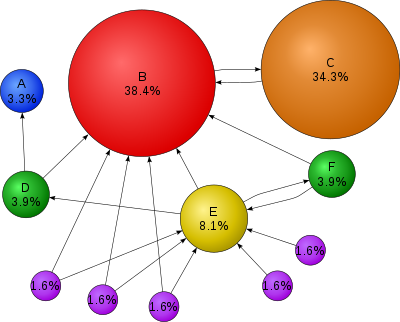
\includegraphics[scale=.5]{400px-PageRanks-Example.png}
\end{center}

Como podemos ver, la página B es relevante porque recibe enlaces desde muchas páginas. La página C en cambio es relevante porque recibe un enlace de B, que es una página relevante. ¿Cómo podemos definir la relevancia?
Pensamos que realizamos el siguiente experimento: ponemos a 1.000.000 de personas a navegar por internet. Inicialmente eligen una página cualquiera al azar y luego cada segundo cambian de página siguiendo algún link al azar de la página en la que están.
Después de varios segundos, ¿cuántos visitantes habrá en cada página?

Podemos modelar esto llamando $\vb^{(0)} \in \R^{11}$ a la cantidad inicial de visitantes en cada sitio, y $\vb^{(k)}$ a la cantidad de visitantes luego de $k$ segundos. Vamos a ver que podemos construir una matriz $\Ab \in \R^{11 \times 11}$, llamada matriz de transición, tal que
$$
\vb^{(k)} = \Ab \vb^{(k-1)}
$$
y recursivamente,
$$
\vb^{(k)} = \Ab^k \vb^{(0)}.
$$

Por lo tanto, para estudiar este proceso, nos interesa poder calcular potencias altas de matrices, o predecir su comportamiento.

Podemos preguntarnos también si existe un límite del proceso, es decir, si luego de varios segundos, la cantidad de visitantes en cada página se mantiene estable. En ese caso, el vector límite debe cumplir la relación
$$
\Ab \vb^{\infty} = \vb^{\infty}.
$$

Los vectores con esta propiedad se llaman autovectores, y es el tema principal de este capítulo.




\section{Autovalores y autovectores}

Dada una matriz cuadrada $\Ab \in \K^{n \times n}$, un vector $\vb \in \K^n$ no nulo tal que
$$
\Ab \vb = \lambda \vb, \text{ para algún } \lambda \in \K
$$ se llama \emph{autovector} de $\Ab$ con \emph{autovalor} $\lambda$.

\textbf{Ejemplo.} Buscamos los autovalores y autovectores de la matriz
$\Ab = \begin{pmatrix} 2 & 3 \\ 2 & 1 \end{pmatrix}$. Tenemos que
encontrar $\vb$ y $\lambda$ tales que $\Ab \vb = \lambda \vb$. El
término de la derecha podemos reescribirlo como $\lambda \Ib \vb$, y esto
nos permite agrupar:
$$(\Ab - \lambda \Ib) \vb = 0,$$
que en nuestro caso queda
$$
\begin{pmatrix}
2 - \lambda & 3 \\
2 & 1 - \lambda
\end{pmatrix}
\begin{pmatrix} v_1 \\ v_2 \end{pmatrix} =
\begin{pmatrix} 0 \\ 0 \end{pmatrix},
$$

Si el determinante de $\Ab - \lambda \Ib$ es no nulo, el sistema tiene
solución única $(v_1, v_2) = (0,0)$. Como estamos buscando vectores no
nulos, debemos encontrar $\lambda$ tal que $\det(\Ab - \lambda \Ib) = 0$.

Calculamos
$$\det(\Ab  - \lambda \Ib) = (2 - \lambda)(1 - \lambda ) - 6 = \lambda^2 - 3 \lambda - 4.$$

Esta ecuación es un polinomio de grado 2 en $\lambda$ y tiene raíces
$$\lambda_1 = -1 \quad \text{y} \quad \lambda_2 = 4.$$
Estos son los autovalores de $\Ab$.

Para calcular los autovectores correspondientes a esos autovalores,
calculamos los núcleos de las matrices $$
\Ab - (-1) \Ib_2 = \begin{pmatrix} 3 & 3 \\ 2 & 2 \end{pmatrix} \quad \text{ y } \quad \Ab - (4) \Ib_2 = \begin{pmatrix} -2 & 3 \\ 2 & -3 \end{pmatrix}.
$$

\begin{Shaded}
\begin{lstlisting}[language=python]
import numpy as np
import scipy.linalg

A = np.array([[2, 3], [2, 1]])
A1 = A - (-1) * np.eye(2)
print(scipy.linalg.null_space(A1))
\end{lstlisting}
\end{Shaded}

\begin{verbatim}
%% [[-0.70710678]
%%  [ 0.70710678]]
\end{verbatim}

\begin{Shaded}
\begin{lstlisting}[language=python]
import numpy as np
import scipy.linalg

A = np.array([[2, 3], [2, 1]])
A1 = A - (-1) * np.eye(2)
print(scipy.linalg.null_space(A1))
\end{lstlisting}
\end{Shaded}

\begin{verbatim}
%% [[0.83205029]
%%  [0.5547002 ]]
\end{verbatim}

El comando \texttt{null\_space} normaliza los vectores a norma-2 igual a 1. Podemos verificar que el espacio de autovectores correspondiente a
$\lambda_1 = -1$ es $$E_{\lambda_1} = \langle (1, -1)\rangle$$ y el
espacio de autovectores correspondiente a $\lambda_2 = 4$ es
$$E_{\lambda_2} = \langle (3, 2)\rangle.$$

Es decir, por ejemplo, $(1, -1)$ es autovector de $\Ab$ de autovalor $-1$,
como también lo es cualquier múltiplo no nulo de ese vector. En este
caso, obtuvimos que el espacio de autovectores de cada autovalor tiene
dimensión 1, o abusando un poco la notación, que a cada autovalor le
corresponde un único autovector.

Repasando,
\begin{itemize}
\item   Los \emph{autovalores} de una matriz $\Ab \in \K^{n \times n}$ ($\K = \R$ o $\C$) son los
    valores $\lambda \in \C$ para los cuales
    $\det(\Ab - \lambda \Ib_n) = 0$.
\item   El espacio de autovalores de un autovalor $\lambda$ es el núcleo de
    la matriz $\Ab - \lambda \Ib_n$.
\item   Si $\lambda$ es autovalor, el núcleo siempre tiene dimensión mayor o
    igual que 1.
\item   Si el núcleo tiene dimensión exactamente 1, decimos informalmente
    que el autovalor $\lambda$ tiene un único autovector.
\end{itemize}

\begin{defi}
Dada $\Ab \in  \Knn$, llamamos \emph{polinomio característico} de $\Ab$ al determinante
$$
\chi_{\Ab}(\lambda) = \det(\Ab - \lambda \Ib).
$$
\end{defi}

Los autovalores de $\Ab$ son las raíces de $\chi_{\Ab}(\lambda)$. El polinomio $\det(\lambda \Ib - \Ab)$ es un polinomio mónico con las mismas raíces que $\det(\lambda \Ib - \Ab)$, y llamamos indistintamente polinomio característico a cualquiera de estos dos polinomios.


\textbf{Ejercicio.} Calcular el polinomio característico, los autovalores y autovectores de la matriz
$$B = \begin{pmatrix} 2 & 0 & 0 \\ 0 & 3 & 4 \\ 0 & 4 & 9 \end{pmatrix}.$$

\textbf{Ejemplo.} Verificamos en \python los cálculos para las dos matrices $\Ab$ y
$\Bb$ utilizando el comando \texttt{linalg.eig} de \texttt{numpy}.

\begin{Shaded}
\begin{lstlisting}[language=python]
A = np.array([[2, 3], [2, 1]])
e = np.linalg.eig(A)   # e es una lista con dos elementos
print("Autovalores: ", e[0])   # El primer elemento es un array
                               # de autovalores
print("Autovectores:\n", e[1]) # El segundo elemento es una matriz
                               # con los autovectores como columnas.
\end{lstlisting}
\end{Shaded}

\begin{verbatim}
%% Autovalores:  [ 4. -1.]
%% Autovectores:
%%  [[ 0.83205029 -0.70710678]
%%  [ 0.5547002   0.70710678]]
\end{verbatim}

\textbf{Ejercicio.} Calcular en \python los autovalores y los autovectores
asociados a cada autovalor para las siguientes matrices.

\begin{enumerate}
\item $\Ab =\begin{pmatrix} -1 & 4 & -2 \\ -3 & 4 & 0 \\ -3 & 1 & 3 \end{pmatrix}$
\item $\Ab = \begin{pmatrix} 0 & 0 & 2 & 1 \\ 1 & 0 & 1 & 0 \\ 0 & 1 & -2 & 0 \\ 0 & 0 & 0 & 1 \end{pmatrix}$
\end{enumerate}

Vamos a utilizar la siguiente propiedad más adelante.

\begin{prop}
Para $\Ab \in \Rnn$, los autovalores de $\Ab$ y $\Ab^T$ son los mismos.
\end{prop}

\begin{proof}
Recordemos que para cualquier $\Ab \in \Rnn$, $\det(\Ab) = \det(\Ab^T)$.

Los autovalores de $\Ab$ son las raíces del polinomio característico $p_{\Ab}(\lambda) = \det(\Ab - \lambda \Ib)$ y los autovalores de $\Ab^T$ son las raíces del polinomio característico $p_{\Ab^T}(\lambda) = \det(\Ab^T - \lambda \Ib)$. Como $(\Ab - \lambda \Ib)^T = \Ab^T - \lambda \Ib$, ambos determinantes son iguales y por lo tanto las raíces son las mismas.
\end{proof}



\section{Diagonalización}

Como vimos, podemos pensar una matriz $\Ab \in \K^{n \times n}$ como una
transformación lineal de $T_{\Ab}: \K^n \rightarrow \K^n$ dada por
$T_{\Ab}(\vb) = \Ab \cdot \vb$ para $\vb \in \K^n$. En este caso estamos pensando
que tanto el vector $\vb$ como $T_{\Ab}(\vb)$ están expresados en coordenadas de
la base canónica. Veamos cómo cambia la matriz de una transformación cuando expresamos los vectores en otra base.

\begin{ejemplo} Continuando el ejemplo anterior, consideramos
$\Ab = \begin{pmatrix} 2 & 3 \\ 2 & 1 \end{pmatrix}$ y la transformación asociada
$$f(\vb) = T_{\Ab}(\vb) = \Ab \vb = \begin{pmatrix} 2 & 3 \\ 2 & 1 \end{pmatrix} \begin{pmatrix} v_1 \\ v_2 \end{pmatrix}.$$

Para esta transformación, vale
$$
\begin{aligned}
T((1,0)) &= (2, 3) \\
T((0,1)) &= (2, 1)
\end{aligned}
$$

También vimos que $\wb_1 = (1,-1)$ y $\wb_2 = (3,2)$ son autovectores de $\Ab$ con autovalores $-1$ y $4$ respectivamente.
Si tomamos la base $\B = \{\wb_1, \wb_2\}$, la transformación en esta base toma una forma más simple:
$$
\begin{aligned}
T(\wb_1) &= -\wb_1 \\
T(\wb_2) &= 4\wb_2
\end{aligned}
$$
o si escribimos a estos vectores en las coordenadas de la base $\B$, obtenemos
$$
\begin{aligned}
T((1,0)_\B) &= (-1,0)_\B \\
T((0,1)_\B) &= (0,4)_\B \\
\end{aligned}
$$

Podemos entonces considerar la matriz de la transformación $T$ expresada en coordenadas de la base $\B$ y llamamos $[f]_\B$ a esta matriz. Obtuvimos:
$$
[f]_\B = \begin{pmatrix} -1 & 0 \\ 0 & 4 \end{pmatrix}.
$$

\end{ejemplo}

En general, tenemos el siguiente resultado.

\begin{prop}
Sea $\Ab \in \Knn$ tal que existe una base $\B = \{\wb_1, \dots, \wb_n\}$ de $\Kn$ formada por autovectores de $\Ab$, con autovalores $\lambda_1, \dots, \lambda_n \in \C$ (no necesariamente distintos). Sea $f: \Kn \rightarrow \Kn$ la transformación asociada, $f(\vb) = \Ab \vb$. La matriz de la $f$ en la base $\B$ es diagonal,
$$
[f]_\B =
\begin{pmatrix} \lambda_1 & & 0 \\ & \ddots & \\ 0 & & \lambda_n \end{pmatrix}
$$

\end{prop}

Estudiamos ahora la relación entre la matriz original $\Ab$ y la matriz $[f]_\B$ en la base de autovectores.

Recordemos que dada una base $\B = \{\wb_1, \dots, \wb_n\}$ de $\Kn$ y un vector $\vb \in \Kn$ con coordenadas en la base $\B$
$$
\vb = (u_1, \dots, u_n)_\B,
$$
podemos encontrar las coordenadas de $\vb$ en la base canónica mediante la multiplicación
$$
\vb_\E = \Cb_{\B\E} \vb_B,
$$
donde $\Cb_{\B\E}$ es la matriz de cambio de base de $\B$ a $\E$,
$$\Cb_{\B\E} = \begin{pmatrix} \mid & \mid & & \mid \\ {\bb}_{1} & {\bb}_{2} & \cdots & {\bb}_{n}\\ \mid & \mid & & \mid \\ \end{pmatrix}.$$

Si en cambio, dadas las coordenadas canónicas de un vector $\vb = (v_1, \dots, v_n)_\E$, queremos encontrar las coordenadas en la base $\B$, realizamos la multiplicación
$$
\vb_\B = \Cb_{\E\B} \vb_E,
$$
donde $\Cb_{\E\B}$ es la matriz de cambio de base de $\E$ a $\B$, que podemos calcular invirtiendo la matriz $\Cb_{\B\E}$,
$$
\Cb_{\E\B} = \Cb_{\B\E}^{-1}.
$$

Por lo tanto, si $f$ es una transformación lineal dada en coordenadas de la base canónica por una matriz $\Ab$, podemos obtener la matriz de la transformación en una base $\B$ (es decir que
tanto $\vb$ como $T_{\Ab}(\vb)$ estén expresados en coordenadas de la base $\B$)
aplicando el siguiente cambio de base a la matriz $\Ab$:
$$
\Ab_\B = \Cb_{\E\B} \Ab \Cb_{\B\E}.
$$

Vemos que tanto $\Ab$ como $\Ab_\B$ representan la misma transformación
lineal pero expresada en distintas bases. En este caso, decimos que las
matrices son \emph{semejantes}.

Más generalmente, dos matrices $\Ab, \Bb$ son \emph{semejantes} si existe una
matriz inversible $\Cb$ tal que
$$\Bb = \Cb^{-1} \Ab \Cb.$$

\textbf{Ejemplo.} Continuamos el ejemplo
$\Ab = \begin{pmatrix} 2 & 3 \\ 2 & 1 \end{pmatrix}$. Vimos que $\Ab$ tiene
autovalores $\lambda_1 = -1$ y $\lambda_2 = 4$ con autovectores
$v_{1} = (1, -1)$ y $v_{2} = (3, 2)$ respectivamente. Estos autovectores
forman una base de $\R^2$. Si expresamos la matriz $\Ab$ en la base
$\Bb = \{v_{1}, v_2\}$ obtenemos
$$
\Ab_\B = \begin{pmatrix} -1 & 0 \\ 0 & 4 \end{pmatrix}
$$
(en las columnas de $\Ab_\B$ ponemos las imágenes de los vectores de la
base $\B$ expresados también en coordenadas de la base $\B$).

Verificamos en \python.

\begin{Shaded}
\begin{lstlisting}[language=python]
A = np.array([[2, 3], [2, 1]])
e = np.linalg.eig(A)
C_BE = e[1]
C_EB = np.linalg.inv(C_BE)
print("A_B = \n", C_EB @ A @ C_BE)
\end{lstlisting}
\end{Shaded}

\begin{verbatim}
%% A_B =
%%  [[ 4.00000000e+00  0.00000000e+00]
%%  [-5.55111512e-17 -1.00000000e+00]]
\end{verbatim}

La siguiente propiedad resume lo que acabamos de ver.

\begin{prop}
Si $\Ab \in \K^{n \times n}$ y $\B = \{\bb_1, \dots, \bb_n\}$
es una base de $\K^n$ formada por autovectores de $\Ab$ con autovalores
$\{\lambda_1, \dots, \lambda_n\}$, entonces tomando

\begin{itemize}
\item   $\Db$ la matriz diagonal de autovalores,
    $\Db = \begin{pmatrix} \lambda_1 & & \\ & \ddots & \\ & & \lambda_n \end{pmatrix}$,
\item   $\Cb$ la matriz de autovectores de $\Ab$,
    $\Cb = \begin{pmatrix} \vert & & \vert \\ \bb_1 & \dots & \bb_n \\ \vert & & \vert \end{pmatrix}$
obtenemos la diagonalización de la matriz $\Ab$
$$
\Ab = \Cb \Db \Cb^{-1} \quad \text{y} \quad \Db = \Cb^{-1} \Ab \Cb.
$$
\end{itemize}
\end{prop}

\textbf{Ejercicio.} Calcular en Python los autovalores y autovectores de las
siguientes matrices. Según los resultados obtenidos, ¿alguna de estas
matrices es diagonalizable?

\begin{enumerate}
\item  $\Ab = \begin{pmatrix} 1 & 1 & 0 \\ 0 & 1 & 1 \\ 0 & 0 & 1 \end{pmatrix}$
\item  $\Ab = \begin{pmatrix} -1 & 3 & -1 \\ -3 & 5 & -1 \\ -3 & 3 & 1 \end{pmatrix}$
\end{enumerate}

Para la matriz que resulte diagonalizable, ¿cuál es la base $\B$ de
autovectores? ¿Quién es $\Db$? Hallar $\Cb$ tal que $\Ab = \Cb \Db \Cb^{-1}$ .

%\begin{lstlisting}[language=R]
%A = matrix(c(1, 1, 0, 0, 1, 1, 0, 0, 1), nrow = 3, byrow = TRUE)
%e = eigen(A)
%print(e)
%
%R(e$vectors)
%print(round(e$vectors, 4))
%\end{lstlisting}
%
%\begin{lstlisting}[language=R]
%A = matrix(c(-1, 3, -1, -3, 5, -1, -3, 3, 1), nrow = 3, byrow = TRUE)
%e = eigen(A)
%print(e)
%
%# Verificamos que tenemos el rango correcto
%R(e$vectors)
%
%#Construimos la matriz diagonal
%D = diag(e$values)
%print(D)
%
%#Construimos las matrices de cambio de base
%
%C = e$vectors
%print(round(C, 4))
%
%C_inv = solve(C)
%
%# Verificamos
%print(C_inv %*% A %*% C)
%print(round(C_inv %*% A %*% C, 4))
%
%print(round(C %*% D %*% C_inv),4)
%
%\end{lstlisting}[language=R]

Como vimos en el ejercicio, no cualquier matriz es diagonalizable.

Dada una matriz $\Ab$, sean $\lambda_1, \dots, \lambda_k$ los autovalores
distintos de $\Ab$. Definimos $E_{\lambda_i}$ el espacio de autovectores
asociados al autovalor $\lambda_i$. $\Ab$ es diagonalizable si
$$
\dim(E_{\lambda_1}) + \dim(E_{\lambda_2}) + \dots +\dim(E_{\lambda_k}) = n.
$$
En particular, como $\dim(E_\lambda) \ge 1$ para $\lambda$ autovector
(¿por qué?), si $\Ab$ tiene $n$ autovalores distintos, $\Ab$ es
diagonalizable.

\begin{ejercicio}
Para cada una de las siguientes matrices, calcular en \python los
autovalores, las dimensiones de los espacios asociados a cada autovalor
y determinar si las matrices son diagonalizables.

\begin{enumerate}
\item   $\Ab = \begin{pmatrix} 101 & 2 & 3 & 4 \\ 1 & 102 & 3 & 4 \\ 1 & 2 & 103 & 4 \\ 1 & 2 & 3 & 104 \end{pmatrix}$
\item   $\Ab = \begin{pmatrix} 5 & 4 & 2 & 1 \\ 0 & 1 & -1 -1 \\ -1 &-1 &3 & 0 \\ 1 & 1 & -1 & 2 \end{pmatrix}$
\end{enumerate}

%\begin{lstlisting}[language=R]
%A = matrix(c(101,2,3,4,1,102,3,4,1,2,103,4,1,2,3,104), nrow=4)
%#A = matrix(c(5,4,2,1,0,1,-1,-1,-1,-1,3,0,1,1,-1,2), nrow=4)
%\end{lstlisting}

\end{ejercicio}

\subsection{Multiplicidad algebraica y geométrica}
Dada una matriz $\Ab \in \Knn$ y un autovalor $\lambda$ de $\Ab$, definimos:
\begin{itemize}
\item La \emph{multiplicidad aritmética} de $\lambda$ es la multiplicidad de $\lambda$ como raíz del polinomio característico $\chi_{\Ab}$.
\item La \emph{multiplicidad geométrica} de $\lambda$ es la dimensión del espacio de autovectores asociado a $\lambda$, o equivalentemente, la dimensión de $\Nu(\Ab - \lambda \Ib)$.
\end{itemize}

\begin{prop}
Dada una matriz $\Ab \in  \Knn$ y un autovalor $\lambda$ de $\Ab$, la multiplicidad geométrica es siempre menor o igual que la multiplicidad aritmética.
\end{prop}

\begin{proof} Sea $s$ la multiplicidad geométrica de $\lambda$ y $\{\vb_1, \dots, \vb_s\}$ una base de autovectores de $E_{\lambda}$, el espacio de autovectores asociados a $\lambda$. Completamos la base de $E_{\lambda}$ a una base de $\Kn$:
$$
\B = \{\vb_1, \dots, \vb_s, \wb_1, \dots, \wb_{n-s}\}.
$$

Consideramos la matriz de la transformación $f$ definida por $\Ab$ en la base $\B$:
$$
\sbox0{$\begin{matrix}\lambda & & \\ & \ddots & \\ & & \lambda\end{matrix}$}
[f]_\B =\left(
\begin{array}{c|c}
\usebox{0}&\makebox[\wd0]{\large $B$}\\
\hline
  \vphantom{\usebox{0}}\makebox[\wd0]{\large $0$}&\makebox[\wd0]{\large $D$}
\end{array}
\right),
$$
donde el primer bloque es una matriz de $s \times s$.

Utilizando la fórmula para el cálculo de determinantes desarrollando una columna, es fácil ver que
$$
\chi_{[f]_\B}(x) = \det(x\Ib_n - [f]_\B) = (x-\lambda)^s \det (x\Ib_n - [f]_\B).$$

 Ya vimos que $[f]_\B$ y $[f]_\E$ tienen el mismo polinomio característico. Por lo tanto, la multiplicidad algebraica de $\lambda$ como autovalor de $\Ab$ es al menos $s$, como queríamos ver.
\end{proof}

Para una matriz $\Ab \in \Knn$, el polinomio característico tiene grado $n$ y por lo tanto $n$ raíces contando sus multiplicidades. Es decir, que la suma de las multiplicidades aritméticas de todos los autovalores es siempre exactamente $n$. Más aún, autovectores correspondientes a autovalores distintos son linealmente independientes.

\begin{prop}
Dada $\Ab \in \Knn$, sean $\vb_1, \dots, \vb_s$ autovectores de $\Ab$ correspondientes a autovalores distintos $\lambda_1, \dots, \lambda_s$.
El conjunto $\{\vb_1, \dots, \vb_s\}$ es linealmente independiente.
\end{prop}

\begin{proof}
Consideramos una relación de dependencia lineal:
$$
a_1 \vb_1 + a_2 \vb_2 + \dots + a_s \vb_s = 0
$$
y supongamos que es la relación que involucra la menor cantidad posible de vectores, en particular todos los $a_i$ son no nulos.

Si multiplicamos la igualdad por $(\Ab - \lambda_1 \Ib_n)$ obtenemos:
$$
a_1  (\Ab - \lambda_1 \Ib_n) \vb_1 + a_2 (\Ab - \lambda_1 \Ib_n) \vb_2 + \dots + a_s(\Ab - \lambda_1 \Ib_n)  \vb_s = 0,$$
y simplificando,
$$
0 + a_2 (\lambda_2 - \lambda_1)  \vb_2 \dots + a_s(\lambda_s - \lambda_1)  \vb_s = 0,
$$
que es una relación con menos términos no nulos que la anterior, lo cual es un absurdo.
\end{proof}

Combinando este resultado con la propiedad anterior, obtenemos el siguiente resultado.

\begin{prop}
Una matriz $\Ab$ es diagonalizable si para todo autovalor $\lambda$ de $\Ab$, la multiplicidad artimética y la multiplicidad geométrica coinciden.
\end{prop}

\

\subsection{Propiedades de las matrices diagonalizables}

\begin{prop} Si $\Ab = \Cb^{-1} \Db \Cb$,
\begin{itemize}
\item   $\Ab^2 = \Cb^{-1} \Db \Cb \Cb^{-1} \Db \Cb = \Cb^{-1} \Db \Db \Cb = \Cb^{-1} \Db^2 \Cb$
\item   Inductivamente, $\Ab^k = \Cb^{-1} \Db \Cb \dots \Cb^{-1} \Db \Cb = \Cb^{-1} \Db^k \Cb$
\item   Si $\Ab$ inversible, $\Ab^{-1} = (\Cb^{-1} \Db \Cb)^{-1} = \Cb^{-1} \Db^{-1} \Cb$.
\item   Si $p(x) \in \R[x]$, $p(\Ab) = \Cb^{-1} p(\Db) \Cb$.
\end{itemize}
\end{prop}

En todos estos casos, como vimos anteriormente, la función aplicada a
una matriz diagonal se puede calcular fácilmente aplicando la función a
cada elemento de la diagonal.


\subsection{Aplicación}

Consideramos el siguiente problema como ejemplo de aplicación.

Para guardar cadenas de caracteres en la computadora se pueden utilizar distintas codificaciones. Una codificación consiste en asignarla a cada carácter un número y ese número se guarda en binario en la memoria de la computadora. Dependiendo la codificación utilizada pueden utilizarse entre 1 y 4 bytes por carácter.
Supongamos ahora que recibimos un mensaje en el que se han mezclado caracteres guardados utilizando 1 byte y caracteres utilizando 2 bytes, y no sabemos cuáles caracteres usan 1 byte y cuáles usan 2 bytes. ¿De cuántas formas distintas se puede interpretar el mensaje?

Planteando el problema en forma más abstracta, tenemos un tablero de $n \times 1$, y queremos dividir el tablero en bloques, que pueden ser de $1 \times 1$ o de $2 \times 1$. ¿De cuántas formas podemos hacerlo?

Llamamos $a_n$ a esta cantidad. Es posible demostrar la siguiente fórmula recursiva para los valores de la sucesión:
$$
\begin{aligned}
a_1 &= 1 \\
a_2 &= 2 \\
a_{n} &= a_{n-1} + a_{n-2}
\end{aligned}
$$

Es decir, los valores $a_n$ forman una sucesión de Fibonacci. Para utilizar la teoría de transformacion lineales, nos gustaría encontrar una relación lineal entre cada término y el siguiente. Sin embargo, como está planteada la sucesión, cada término depende de los dos anteriores. Aplicamos un truco simple para plantear la relación de forma que cada término dependa solo del anterior. Plantear la ecuación de recurrencia en forma matricial de la siguiente forma:
$$
\begin{pmatrix} a_{n} \\ a_{n-1} \end{pmatrix} =
\begin{pmatrix} 1 & 1 \\ 1 & 0 \end{pmatrix} \begin{pmatrix} a_{n-1} \\ a_{n-2} \end{pmatrix}.
$$

Si llamamos $\Ab = \begin{pmatrix} 1 & 1 \\ 1 & 0 \end{pmatrix}$, obtenemos
$$
\begin{pmatrix} a_{n} \\ a_{n-1} \end{pmatrix} =
\Ab \begin{pmatrix} a_{n-1} \\ a_{n-2} \end{pmatrix} = \Ab \Ab \begin{pmatrix} a_{n-2} \\ a_{n-3} \end{pmatrix} = \dots = (\Ab)^{n-2} \begin{pmatrix} a_{2} \\ a_{1} \end{pmatrix}
$$

Por lo tanto, podemos dar una fórmula cerrada para la sucesión si encontramos una expresión cerrada para la matriz $(\Ab)^{n-2}$. Esto podemos hacerlo diagonalizando la matriz.

Calculamos autovalores y autovectores de $\Ab$ en \python.

\begin{Shaded}
\begin{lstlisting}[language=python]
A = np.array([[1, 1], [1, 0]])
e = np.linalg.eig(A)
print("Autovalores: ", e[0])
print("Autovectores: \n", e[1])
\end{lstlisting}
\end{Shaded}

\begin{verbatim}
%% Autovalores:  [ 1.61803399 -0.61803399]
%% Autovectores:
%%  [[ 0.85065081 -0.52573111]
%%  [ 0.52573111  0.85065081]]
\end{verbatim}

Como hay dos autovalores distintos, podemos diagonalizar $\Ab$. Obtenemos
$$
\Ab = \Cb_{\B\E} \begin{pmatrix} 1.618 & 0 \\ 0 & -0.618 \end{pmatrix} \Cb_{\E\B},
$$
con $\Cb_{\B\E} = \begin{pmatrix} 0.85 & -0.52 \\ 0.52 & 0.85 \end{pmatrix}$ y $\Cb_{\E\B} = \Cb_{\B\E}^{-1}$.

Esto nos permite dar la siguiente expresión para los términos de la sucesión:
$$
\begin{pmatrix} a_{n} \\ a_{n-1} \end{pmatrix} =
\Cb_{\B\E} \begin{pmatrix} (1.618)^{n-2} & 0 \\ 0 & (-0.618)^{n-2} \end{pmatrix} \Cb_{\E\B} \begin{pmatrix} a_{2} \\ a_{1} \end{pmatrix}.
$$

Vemos en particular que los términos de la sucesión crecen con velocidad exponencial. Haciendo las cuentas en forma simbólica, podemos dar una expresión exacta para los términos de la sucesión (los autovalores de la matriz son $\frac{1+\sqrt{5}}{2} y \frac{1-\sqrt{5}}{2}$.










\section{Descomposición de Schur}
Si bien vimos que no toda matriz es diagonalizable, es decir, semejante a una matriz diagonal, vamos a ver que toda la matriz es semejante a una matriz triangular superior con los autovalores en la diagonal. Más aun, la matriz de cambio de base se puede tomar unitaria. En este caso, decimos que las matrices son unitariamente equivalentes. Concretamente, tenemos el siguiente resultado.

\begin{teo}
Dada una matriz $\Ab \in \Knn$ con autovalores $\lambda_1, \dots, \lambda_n$ (no necesariamente distintos), existen matrices $\Ub$ unitaria y $\Tb$ triangular superior tales que
$$
\Ab = \Ub \Tb \Ub^*
$$
y $t_{ii} = \lambda_i$. Es decir, $\Ab$ es unitariamente equivalente a una matriz $\Tb$ triangular superior con los autovalores de $\Ab$ en la diagonal en cualquier orden arbitrario. Si $\Ab \in \Rnn$ y los autovalores de $\Ab$ son reales, la matriz $\Ub$ se puede tomar real y ortogonal.
\end{teo}

Recordemos que para una matriz $\Ub$ unitaria, vale $\Ub^{-1} = \Ub^*$, por lo tanto las matrices $\Ab$ y $\Tb$ son semejantes.

\begin{proof}
Construimos $\Ub$ y $\Tb$ paso a paso.

Tomamos $\lambda_1$ autovalor de $\Ab$ y $\wb_1$ autovector de $\Ab$ con autovalor $\lambda_1$ y $\|\wb_1\|_2 = 1$.

Completando $\{\wb_1\}$ a una base de $\Kn$ y aplicando ortonormalización de Gram-Schmidt, podemos obtener una base ortonormal de $\C^n$,
$$
\{\wb^{(1)}, \zb^{(2)}, \dots, \zb^{(n)}\}.
$$

Construimos la matriz $\Ub_1$ tomando estos vectores como columnas de la matriz. Como la primera columna de $\Ab \Ub_1$ es $\lambda_1 \wb^{(1)}$, obtenemos
$$
\Ub_1^* \Ab \Ub_1 = \left[
\begin{array}{c|c}
\lambda_1 & * \\ \hline
0 & \Ab_1
\end{array}
\right],
$$

Como $\Ub_1^* \Ab \Ub$ y $\Ab$ son semejantes, tienen el mismo polinomio característico. Luego $\Ab_1 \in \C^{(n-1) \times (n-1)}$ tiene autovalores $\lambda_2, \dots, \lambda_n$. Tomamos ahora $\wb^{(2)} \in \C^{n-1}$ autovector normalizado de $\Ab_1$ correspondiente al autovalor $\lambda_2$ y repetimos el procedimiento. Construimos $\Ub_2 \in \C^{(n-1) \times (n-1)}$ unitaria tal que
$$
\Ub_2^* \Ab_1 \Ub_2 = \left[
\begin{array}{c|c}
\lambda_2 & * \\ \hline
0 & \Ab_2
\end{array}
\right],
$$
y definimos
$$
\Vb_2 = \left(
\begin{array}{c|c}
1 & 0 \\ \hline
0 & \Ub_2
\end{array}
\right).
$$

Las matrices $\Vb_2$ y $\Ub_1 \Vb_2$ son unitarias, y $\Vb_2^* \Ub_1^* \Ab \Ub_1 \Vb_2$ tiene la forma
$$
\sbox0{$\begin{matrix}\lambda_1 & * \\ 0 & \lambda_2 \end{matrix}$}
\Vb_2^* \Ub_1^* \Ab \Ub_1 \Vb_2 =\left(
\begin{array}{c|c}
\usebox{0}& \makebox[\wd0]{\large $*$}\\
\hline
    \vphantom{\usebox{0}}\makebox[\wd0]{\large $0$}&\makebox[\wd0]{\large $\Ab_2$}
\end{array}
\right).
$$

Repitiendo este procedimiento, obtenemos matrices unitarias $\Ub_i \in \C^{(n-i+1) \times (n-i+1)}$, $i = 1, \dots, n-1$, y matrices unitarias $\Vb_i \in \Cnn$, $i = 2, \dots, n-1$. La matriz
$$
\Ub = \Ub_1 \Vb_2 \Vb_3 \dots \Vb_{n-1}
$$
es unitaria y $\Ub^* \Ab \Ub$ es la factorización que buscamos.

Si todos los autovalores de $\Ab$ son reales, los autovectores pueden elegirse también reales y todas las operaciones se pueden hacer sobre los reales, lo que prueba la última información.
\end{proof}

\section{Autovalores y autovectores de matrices simétricas y hermitianas}

\textbf{Matrices ortogonales.} Si $\Ab \in \K^{n \times n}$ es unitaria,
    todos sus autovalores cumplen $|\lambda| = 1$.

\textbf{Matrices normales.}
Decimos que una matriz $\Ab$ es normal si conmuta con la matriz adjunta, es decir, si $\Ab \Ab^* = \Ab^* \Ab$.

Recordemos que dos matrices $\Ab$ y $\Bb$ son unitariamente equivalentes si existe $\Ub$ unitaria tal que
$$
\Ub^* \Ab \Ub = \Bb.
$$

\begin{prop}
Si $\Ab$ es normal y $\Bb$ es unitariamente equivalente a $\Ab$, entonces $\Bb$ es normal.
\end{prop}
\begin{proof}
Tenemos que existe $\Ub$ unitaria tal que $\Ub^* \Ab \Ub = \Bb$. Por lo tanto,
$$
\Bb \Bb^* = \Ub^* \Ab \Ub \Ub^* \Ab^* \Ub = \Ub^* \Ab \Ab^* \Ub = \Ub^* \Ab^* \Ab \Ub = \Ub^* \Ab^* \Ub \Ub^* \Ab \Ub = \Bb^* \Bb.
$$
\end{proof}

Decimos que una matriz $\Ab$ es \emph{unitariamente diagonalizable} si existe una matriz $\Ub$ unitaria tal que $\Ub \Ab \Ub^*$ es diagonal. Esto es equivalente a decir que $\Ab$ tiene una base ortonormal de autovectores.

\begin{prop}
Si $\Ab$ es normal, entonces $\Ab$ es unitariamente diagonalizable. En particular, autovectores de $\Ab$ correspondientes a autovalores distintos son ortogonales.
\end{prop}

\begin{proof}
Por la descomposición de Shur, sabemos que existe $\Tb$ triangular superior unitariamente equivalente a $\Ab$.
Por lo tanto, podemos probar el resultado para $\Tb$.

Hacemos la demostración probando mediante cálculos explícitos que una matriz $\Tb$ triangular y normal debe ser diagonal. Tenemos
$$
\begin{pmatrix}
\bar t_{11} & 0           & \cdots & 0 \\
\bar t_{21} & \bar t_{22} & \cdots & 0\\
\vdots      & \vdots      & \ddots & \vdots \\
\bar t_{n1} & \bar t_{n2} & \cdots & \bar t_{nn}\\
\end{pmatrix}
\begin{pmatrix}
t_{11} & t_{12} & \cdots & t_{1n} \\
0      & t_{22} & \cdots & t_{2n} \\
\vdots & \vdots & \ddots & \vdots \\
0      & 0      & \cdots & t_{nn}\\
\end{pmatrix} =
\begin{pmatrix}
t_{11} & t_{12} & \cdots & t_{1n} \\
0      & t_{22} & \cdots & t_{2n} \\
\vdots & \vdots & \ddots & \vdots \\
0      & 0      & \cdots & t_{nn}\\
\end{pmatrix} \begin{pmatrix}
\bar t_{11} & 0           & \cdots & 0 \\
\bar t_{21} & \bar t_{22} & \cdots & 0\\
\vdots      & \vdots      & \ddots & \vdots \\
\bar t_{n1} & \bar t_{n2} & \cdots & \bar t_{nn}\\
\end{pmatrix}.
$$

Comparando la casilla $(1,1)$ del producto a ambos lados,
$$
\bar t_{11} t_{11} = t_{11} \bar t_{11} + \sum_{j = 2}^n t_{1j} \bar t_{j1}.
$$
Recordando que para cualquier $a \in \C$, $a \bar a = \bar a a = |a|^2$, obtenemos
$$
|t_{11}|^2 = |t_{11}|^2  + \sum_{j = 2}^n |t_{1j}|^2.
$$
y por lo tanto
$$
0 = \sum_{j = 2}^n |t_{1j}|^2.
$$
Una suma de términos no-negativos solo puede dar 0 si todos sus términos son 0, luego
$$
t_{1j} = 0, j = 2, \dots, n.
$$

Ahora usamos que la casillas $(2,2)$ de $\Tb^* \Tb$ y $\Tb \Tb^*$ son iguales y obtenemos
$$
\bar t_{22} t_{22} = t_{22} \bar t_{22} + \sum_{j = 3}^n t_{2j} \bar t_{j2},
$$
de donde concluimos
$$
t_{2j} = 0, j = 3, \dots, n.
$$

Repitiendo este mismo argumento para todas las casillas de la diagonal, obtenemos
$$
t_{ij} = 0, \text{ para todo } j > i
$$
y como
$$
t_{ij} = 0, \text{ para todo } j < i
$$
porque $\Tb$ es triangular superior, concluimos que $\Tb$ es diagonal.
\end{proof}




\textbf{Matrices simétricas y hermitianas.} Una matriz $\Ab \in \Rnn$ es simétrica si $\Ab = \Ab^T$. Más generalmente, $\Ab \in \Cnn$ es Hermitiana si $\Ab = \Ab^*$.

\begin{prop}
Si $\Ab$ es Hermitiana, entonces
\begin{enumerate}
\item \label{item:real} $\xb^* \Ab \xb$ es real para todo $\xb \in \Cn$,
\item \label{item:realav} todos los autovalores de $\Ab$ son reales,
\item $\Sb^* \Ab \Sb$ es Hermitiana para toda $\Sb \in \Cnn$.
\end{enumerate}
\end{prop}

\begin{proof}
Para \ref{item:real}, calculamos
$$
\overline{\xb^* \Ab \xb} = (\xb^* \Ab \xb)^* = \xb^* \Ab^* \xb = \xb^* \Ab \xb.
$$
Como el conjugado de $\xb^* \Ab \xb$ es igual a si mismo, es un n\'umero real.

Para \ref{item:realav}, si $\Ab \xb = \lambda \xb$ y suponemos $\xb$ normalizado $\|\xb\|_2 = \xb^* \xb = 1$, entonces
$$\lambda = \lambda \xb^* \xb = \xb^* \lambda  \xb =  \xb^* \Ab  \xb,$$
que es un n\'umero real por \ref{item:real}.

Por \'ultimo, $(\Sb^* \Ab \Sb)^* = \Sb^* \Ab^* \Sb = \Sb^* \Ab \Sb$, y por lo tanto $\Sb^* \Ab \Sb$ es Hermitiana.
\end{proof}

\begin{ejemplo}
Buscamos una base ortogonal de autovectores de
$$
\Ab = \begin{pmatrix} -4 & 2 & -2 \\ 2 & -7 & 4 \\ -2 & 4 & -7 \end{pmatrix}.$$

Calculamos $\det(\Ab - \lambda \Ib_3) = -(\lambda^3 + 18 \lambda^2 + 81 \lambda + 108) = -(\lambda + 12)(\lambda + 3)^2$, por lo tanto hay dos autovalores $\lambda_1 = -12$ y $\lambda_2 = -3$.

Calculando los núcleos de $\Ab - \lambda_i \Ib_3$, $i = 1, 2$, obtenemos los espacios de autovectores
$$
\begin{aligned}
E_{\lambda_1} &= \langle (1, -2, 2) \rangle \\
E_{\lambda_2} &= \langle (2, 1, 0), (2, 0, -1) \rangle
\end{aligned}
$$

Por la Proposición \ref{prop:normal}, los espacios de autovalores correspondientes a distintos autovectores son ortogonales. Por lo tanto, para obtener una base de autovectores ortogonales, solo debemos ortogonalizar cada uno de los autoespacios por separado.

El autovector $(1, -2, 2)$ lo normalizamos a $\frac{\sqrt{5}}{5}(1, -2, 2)$ y para encontrar una base ortonormal de $E_{\lambda_2}$ aplicamos Gram-Schmidt y obtenemos $E_{\lambda_2} = \left\langle \frac{\sqrt{3}}{3}(2, 1, 0), \frac{\sqrt{5}}{15}(2, -4, -5) \right\rangle$.

La base ortogonal de autovectores es $\B = \left\{\frac{\sqrt{5}}{5}(1, -2, 2), \frac{\sqrt{3}}{3}(2, 1, 0), \frac{\sqrt{5}}{15}(2, -4, -5)\right\}$.
\end{ejemplo}



\begin{ejercicio} Calcular los autovalores y autovectores de las siguientes
matrices.

\begin{itemize}
\item   $\Ab = \begin{pmatrix} 1 & 0 & 0 \\ 0 & \cos \alpha & -\sin \alpha \\ 0 & \sin \alpha & \cos \alpha \end{pmatrix}$,
    para $\alpha = \pi/2$ y $\alpha = \pi / 4$.
\item  $\Ab = \begin{pmatrix} 0 & 0 & -2 \\ 0 & -2 & 0 \\ -2 & 0 & -3 \end{pmatrix}$
\end{itemize}

En el segundo punto, encontrar una matriz $\Qb$ ortogonal y una matriz $\Db$
diagonal tales que $\Ab = \Qb^T \Db \Qb$.

\end{ejercicio}

\subsection{Matrices definidas positivas}

Cuando $\Ab$ es simétrica, con autovalores $\lambda_1, \dots, \lambda_n$ ,
definimos:

\begin{itemize}
\item   $\Ab$ es \emph{definida positiva} si $\lambda_i(\Ab) > 0$ para todo
    $1 \le i \le n$.
\item  $\Ab$ es \emph{semidefinida positiva} si $\lambda_i(\Ab) \ge 0$ para todo
    $1 \le i \le n$.
\end{itemize}

\begin{prop}

\item   $\Ab \in \R^{n \times n}$ es \emph{semidefinida positiva} si y solo si
    $\vb^T \Ab \vb \ge 0$ para todo $\vb \in \R^n$.

\textbf{Demostración / ejemplo:}

Si $\Ab = \begin{pmatrix} \lambda_1 & 0 \\ 0 & \lambda_2 \end{pmatrix}$, y
$v = (v_1, v_2)$,
$$ \begin{aligned} \vb^T \Ab \vb &=
\begin{pmatrix} v_1 & v_2 \end{pmatrix} \begin{pmatrix} \lambda_1 & 0 \\ 0 & \lambda_2 \end{pmatrix} \begin{pmatrix} v_1 \\ v_2 \end{pmatrix} \\
&= \begin{pmatrix} v_1 & v_2 \end{pmatrix} \begin{pmatrix} \lambda_1 v_1 \\ \lambda_2 v_2\end{pmatrix} \\
&= \begin{pmatrix} \lambda_1 v_1^2 + \lambda_2 v_2^2 \end{pmatrix},
\end{aligned}$$
y $\lambda_1 v_1^2 + \lambda_2 v_2^2 \ge 0$ si
$\lambda_1, \lambda_2 \ge 0$.

\end{prop}

\begin{prop}
 $\Ab^T\Ab$ y $\Ab\Ab^T$ son matrices simétricas y semidefinidas positivas.
 \end{prop}

\begin{proof}Ejercicio.\end{proof}

\section{El método de la potencia}

Veamos cómo podemos calcular mediante aproximaciones numéricas los autovalores de una matriz.

Comencemos con un ejemplo. Consideremos la matriz
$$
A = \begin{pmatrix}
0.9 & 0.075 & 0.025 \\
0.15 & 0.8 &  0.05 \\
0.25 & 0.25 & 0.5
\end{pmatrix}
$$

Tomamos un vector cualquiera no nulo, por ejemplo $\vb = (1, 2, 3)$ y calculamos $\Ab^k \vb$ para distintos valores de $k$.
O, equivalentemente, calculamos distintos términos de la sucesión definida recursivamente por
$$
\begin{aligned}
\vb^{(0)} &= (1,2,3) \\
\vb^{(k)} &= \Ab \vb^{(k-1)}
\end{aligned}
$$

Lo programamos en \python.

\begin{Shaded}
\begin{lstlisting}[language=python]
def estado(A, v, k):
    for i in range(k):
        v = A @ v
    return(v)

A = np.array([[0.9, 0.075, 0.025], [0.15, 0.8, 0.05], [0.25, 0.25, 0.5]])
v = np.array([1,2,3])
print(estado(A, v, 1))
print(estado(A, v, 10))
print(estado(A, v, 100))
print(estado(A, v, 1000))
\end{lstlisting}
\end{Shaded}

\begin{verbatim}
%% [1.125 1.9   2.25 ]
%% [1.41762971 1.47373372 1.45503428]
%% [1.4375 1.4375 1.4375]
%% [1.4375 1.4375 1.4375]
\end{verbatim}

Observamos en el experimento que $\vb^{(k)}$ tiende a $\wb = (1.4375, 1.4375, 1.4375)$. Si esto es cierto, entonces $\Ab \wb = \wb$. Luego encontramos un autovector de autovalor 1. ¿C\'omo podemos demostrar lo que observamos?

Calculamos autovalores y autovectores de $\Ab$ y verificamos si $\Ab$ es diagonalizable.

\begin{Shaded}
\begin{lstlisting}[language=python]
e = np.linalg.eig(A)
print(e[0])
print(e[1])
\end{lstlisting}
\end{Shaded}

\begin{verbatim}
%% [1.         0.74142136 0.45857864]
%% [[-0.57735027 -0.44371857 -0.03400257]
%%  [-0.57735027  0.81130706 -0.13017638]
%%  [-0.57735027  0.38065035  0.99090763]]
\end{verbatim}

Obtenemos que $\Ab$ es diagonalizable con autovalores $\lambda_1 = 1$, $\lambda_2 = 0.74$, $\lambda_3 = 0.45$. Llamamos $\B = \{\wb_1, \wb_2, \wb_3\}$ a la base de autovectores.

Luego podemos escribir a cualquier vector  $\vb^{(0)} \in \R^3$ como combinación lineal de vectores de la base $\B$:
$$
\vb^{(0)} = a_1 \wb_1 + a_2 \wb_2 + a_3 \wb_3.
$$

Usando esta representación, ¿quién es $\Ab \vb^{(0)}$? Obtenemos
$$
\begin{aligned}
\vb^{(1)} = \Ab \vb^{(0)} &= a_1 \Ab \wb_1 + a_2 \Ab \wb_2 + a_3 \Ab \wb_3 \\
        &= a_1 \lambda_1 \wb_1 + a_2  \lambda_2  \wb_2 + a_3  \lambda_3 \wb_3
\end{aligned}
$$
y si multiplicamos nuevamente por $\Ab$,
$$
\begin{aligned}
\vb^{(2)} = \Ab^2 \vb = \Ab (\Ab \vb) &= a_1 \Ab \lambda_1 \wb_1 + a_2  \Ab \lambda_2  \wb_2 + a_3  \Ab \lambda_3 \wb_3\\
        &= a_1 \lambda_1^2 \wb_1 + a_2  \lambda_2^2  \wb_2 + a_3  \lambda_3^2 \wb_3
\end{aligned}
$$

Repitiendo el mismo razonamiento obtenemos
$$
\vb^{(k)} = \Ab^k \vb = a_1 (\lambda_1)^k \wb_1 + a_2 (\lambda_2)^k  \wb_2 + a_3 (\lambda_3)^k \wb_3.
$$

Como $|\lambda_2| < 1$ y $|\lambda_3|< 1$, tenemos que $(\lambda_2)^k \xrightarrow[k \rightarrow \infty]{} 0$ y $(\lambda_3)^k \xrightarrow[k \rightarrow \infty]{} 0$. Por otro lado, $\lambda_1^k = 1$ para todo $k \in \N$.

Tomando límite, concluimos entonces
$$
\vb^{(k)} \xrightarrow[k \rightarrow \infty]{} a_1 \wb_1,
$$
es decir $\vb^{(k)}$ tiende a un vector de autovalor 1, que es el autovalor de mayor módulo de la matriz.

En general, las matrices pueden tener autovalores de cualquier módulo y la sucesión anterior podría tender a $\cero$ o diverger o no tener límite. Para el caso general, realizamos la siguiente modificación.

Tomamos un vector cualquiera no nulo $\vb^{(0)}$ y en cada iteración de la recursión anterior normalizamos el resultado a norma-2 $= 1$:
$$
\begin{aligned}
\vb^{(k)} &= \frac{\Ab \vb^{(k-1)}}{\|\Ab\vb^{(k-1)}\|_2}, \text{ para } k \ge 1.
\end{aligned}
$$

Calculamos en \python los vectores de esta sucesión tomando $\vb^{(0)} = (1, 2, 3)$ y
$$
\Ab = \begin{pmatrix}
3 & 1 & 2 \\
0 & 1 & -2 \\
1 & 2 & 4
\end{pmatrix}
$$


\begin{Shaded}
\begin{lstlisting}[language=python]
def estado(A, v, k):
    for i in range(k):
        Av = A @ v
        v = Av / np.linalg.norm(Av, 2)
    return(v)
A = np.array([[3, 1, 2], [0, 1, -2], [1, 2, 4]])
v = np.array([1,2,3])
print(estado(A, v, 1))
print(estado(A, v, 10))
print(estado(A, v, 100))
print(estado(A, v, 1000))
\end{lstlisting}
\end{Shaded}

\begin{verbatim}
%% [ 0.53295174 -0.19380063  0.82365269]
%% [ 0.74404261 -0.37049752  0.55599656]
%% [ 0.74278135 -0.37139068  0.55708601]
%% [ 0.74278135 -0.37139068  0.55708601]
\end{verbatim}

Observamos que en este caso también existe límite $\vb^{(k)} \xrightarrow[k \rightarrow \infty]{} \wb = (2.97, -1.49,  2.23)$. ¿Será cierto en este caso también que $\wb$ es un autovector? ¿Cuál es el autovalor correspondiente? Para responder estas preguntas, utilizamos nuevamente que si $\wb$ es el l\'imite de la sucesión, al aplicar la fórmula recursiva a $\wb$ obtenemos nuevamente $\wb$. Es decir,
$$
\wb = \frac{\Ab \wb}{\|\Ab \wb\|_2},
$$
y despejando, obtenemos
$$
\Ab \wb = \|\Ab \wb\|_2 \wb.
$$
Concluimos que $\wb$ es autovector de $\Ab$ con autovalor $\lambda = \|\Ab \wb\|_2 = 4$ (verificar esta última cuenta en \python).

Para demostrar el resultado en este caso, calculamos nuevamente autovalores y autovectores de $\Ab$:
\begin{Shaded}
\begin{lstlisting}[language=python]
e = np.linalg.eig(A)
print(e[0])
print(e[1])
\end{lstlisting}
\end{Shaded}

\begin{verbatim}
%% [4.+0.j 2.+1.j 2.-1.j]
%% [[ 0.74278135+0.j          0.35355339-0.35355339j  0.35355339+0.35355339j]
%%  [-0.37139068+0.j         -0.70710678+0.j         -0.70710678-0.j        ]
%%  [ 0.55708601+0.j          0.35355339+0.35355339j  0.35355339-0.35355339j]]
\end{verbatim}

Nuevamente la matriz es diagonalizable con autovalores $\lambda_1 = 4$, $\lambda_2 = 2 + i$, $\lambda_3 = 2-i$.
Aplicando el razonamiento anterior,
$$
\begin{aligned}
\vb^{(1)} &= \frac{\Ab \vb^{(0)}}{\|\Ab\vb^{(0)}\|_2}, \\
\vb^{(2)} &= \frac{\Ab \vb^{(1)}}{\|\Ab\vb^{(1)}\|_2} =
 \frac{\Ab \frac{\Ab \vb^{(0)}}{\|\Ab\vb^{(0)}\|_2}}{\left\|\Ab \frac{\Ab \vb^{(0)}}{\|\Ab\vb^{(0)}\|_2}\right\|_2} =
 \frac{\frac{\Ab^2 \vb^{(0)}}{\|\Ab\vb^{(0)}\|_2}}{\frac{\|\Ab^2 \vb^{(0)}\|_2}{\|\Ab\vb^{(0)}\|_2}} =
 \frac{\Ab^2 \vb^{(0)}}{\|\Ab^2 \vb^{(0)}\|_2} \\
 &\dots \\
\vb^{(k)} &=  \frac{\Ab \vb^{(k-1)}}{\|\Ab\vb^{(k-1)}\|_2} = \frac{\Ab^k \vb^{(0)}}{\|\Ab^k\vb^{(0)}\|_2}.
\end{aligned}$$

Obtenemos en este caso,
$$
\begin{aligned}
\vb^{(k)} &= \frac{\Ab^k \vb^{(0)}}{\|\Ab^k\vb^{(0)}\|_2}  \\
&= \frac{a_1 (\lambda_1)^k \wb_1 + a_2 (\lambda_2)^k  \wb_2 + a_3 (\lambda_3)^k \wb_3}{\|a_1 (\lambda_1)^k \wb_1 + a_2 (\lambda_2)^k  \wb_2 + a_3 (\lambda_3)^k \wb_3\|_2}  \\
&=\frac{\lambda_1^k\left(a_1 \wb_1 + a_2 \left(\frac{\lambda_2}{\lambda_1}\right)^k  \wb_2 + a_3 \left(\frac{\lambda_3}{\lambda_1}\right)^k \wb_3\right)}{|\lambda_1|^k \left\|a_1 \wb_1 + a_2 \left(\frac{\lambda_2}{\lambda_1}\right)^k  \wb_2 + a_3 \left(\frac{\lambda_3}{\lambda_1}\right)^k \wb_3\right\|_2} \\
&= \left(\frac{\lambda_1}{|\lambda_1|}\right)^k \frac{a_1 \wb_1 + a_2 \left(\frac{\lambda_2}{\lambda_1}\right)^k  \wb_2 + a_3 \left(\frac{\lambda_3}{\lambda_1}\right)^k \wb_3}{\left\|a_1 \wb_1 + a_2 \left(\frac{\lambda_2}{\lambda_1}\right)^k  \wb_2 + a_3 \left(\frac{\lambda_3}{\lambda_1}\right)^k \wb_3\right\|_2}
\end{aligned}$$

En nuestro ejemplo, $\lambda_1 = 4$ y $\left(\frac{\lambda_1}{|\lambda_1|}\right)^k = 1$. Los cocientes $\lambda_i / \lambda_1$, $i = 2, 3$ tienden a $0$ y por lo tanto $\vb^{(k)}$ tiende a $\wb_1 / \|\wb_1\|_2$.

Observamos que si $\lambda_1$ no es un número real positivo, $\lambda_1/|\lambda_1|$ es un número (complejo) de módulo 1, y $(\lambda_1 / |\lambda_1|)^k$ tiene módulo 1 para todo $k$ pero no tiene límite. Sin embargo, a partir de esta sucesión podemos aproximar el valor de $\lambda_1$ y conociendo $\lambda_1$ podemos obtener fácilmente un autovector correspondiente a este autovalor. Esta estrategia para calcular el autovalor de módulo máximo se conoce como el \emph{método de la potencia}. Vamos a presentar el método realizando algunas suposiciones que facilitan la demostración. El método se puede aplicar en condiciones más generales, incluso cuando $\Ab$ no es diagonalizable, pero en ese caso necesitamos utilizar la forma de Jordan de la matriz u otras herramientas que escapan el contenido de este apunte para la demostración.

%\begin{algorithm}
%\end{algorithm}

\begin{lema}
Si $\vb$ es un autovector de $\Ab \in \Cnn$ de autovalor $\lambda$, el cociente de Rayleigh
$$
r(\vb) = \frac{\vb^T \Ab \vb}{\vb^T \vb}
$$
es igual al autovalor $\lambda$.
\end{lema}

La demostración es inmediata usando que si $\vb$ es autovector de autovalor $\lambda$, $\Ab \vb = \lambda \vb$.
A partir de la definición tenemos muchas formas de calcular el autovalor correspondiente a un autovector. Se puede demostrar que cuando tenemos una aproximación $\vb$ de un autovector, $r(\vb)$ es el valor que más se parece a un autovalor, en el sentido de que $\alpha = r(\vb)$ minimiza la norma de $\|\Ab\vb - \alpha \vb\|_2$.

\begin{algorithm}[H]
\SetAlgoLined
$\Ab \in \C^{n \times n}$, $\vb^{(0)} \in \C^n$\;
%\KwResult{Write here the result }
 \For{$k = 1, 2, \dots$}{
  $\vb^{(k)} = \frac{\Ab \vb^{(k-1)}}{\|\Ab\vb^{(k-1)}\|_2}$\;
  $r_k = \frac{(\vb^{(k)})^T \Ab \vb^{(k)}}{(\vb^{(k)})^T \vb^{(k)}}$
 }
 \caption{Método de la potencia}
\end{algorithm}


\begin{teo}
Sea $\Ab \in \Cnn$ una matriz diagonalizable con base de autovectores $\B = \{\wb_1, \dots, \wb_n\}$ y autovalores correspondientes $\{\lambda_1, \dots, \lambda_n\}$ con $|\lambda_1| > |\lambda_2| \ge \dots \ge |\lambda_n| \ge 0$ (existe un único autovalor de módulo máximo). Dado un vector $\vb^{(0)} \in \C^n$ tal que en su escritura en la base $\B$ el coeficiente de $\wb_1$ es no nulo, el algoritmo \ref{} satisface $|r_k - \lambda_1| \rightarrow 0$ cuando $k \rightarrow \infty$.
\end{teo}

\begin{proof}
Por hipótesis, podemos escribir
$$
\vb^{(0)} = a_1 \wb_1 + \dots + a_n \wb_n,
$$
con $a_1 \neq 0$.
Siguiendo los pasos del ejemplo, obtenemos
$$
\vb^{(k)} = \left(\frac{\lambda_1}{|\lambda_1|}\right)^k \frac{a_1 \wb_1 + a_2 \left(\frac{\lambda_2}{\lambda_1}\right)^k \wb_2 + \dots + a_n \left(\frac{\lambda_n}{\lambda_1}\right)^k \wb_n}{\left\|a_1 \wb_1 + a_2 \left(\frac{\lambda_2}{\lambda_1}\right)^k  \wb_2 + \dots + a_n \left(\frac{\lambda_n}{\lambda_1}\right)^k \wb_n\right\|_2}.
$$

Despejando,
$$
\left(\frac{|\lambda_1|}{\lambda_1}\right)^k \vb^{(k)} = \frac{a_1 \wb_1 + a_2 \left(\frac{\lambda_2}{\lambda_1}\right)^k \wb_2 + \dots + a_n \left(\frac{\lambda_n}{\lambda_1}\right)^k \wb_n}{\left\|a_1 \wb_1 + a_2 \left(\frac{\lambda_2}{\lambda_1}\right)^k \wb_2 + \dots + a_n \left(\frac{\lambda_n}{\lambda_1}\right)^k \wb_n\right\|_2}
$$
y por lo tanto, llamando $\tilde \vb^{(k)} = \left(\frac{|\lambda_1|}{\lambda_1}\right)^k \vb^{(k)}$,
$$
\tilde \vb^{(k)} \xrightarrow[k \rightarrow \infty]{} \frac{a_1 \wb_1}{\left\|a_1 \wb_1\right\|_2}.
$$

Como $\tilde \vb^{(k)}$ es igual a $\vb^{(k)}$ multiplicado por un escalar, podemos fácilmente ver que
$$
r(\tilde \vb^{(k)}) = \frac{(\tilde \vb^{(k)})^T \Ab \tilde \vb^{(k)}}{(\tilde \vb^{(k)})^T  \tilde \vb^{(k)}} = \frac{(\vb^{(k)})^T \Ab \vb^{(k)}}{( \vb^{(k)})^T  \vb^{(k)}} = r(\vb^{(k)}).
$$

%y concluimos que
%$$
%\lim_{k \rightarrow \infty} \frac{(\vb^{(k)})^T \Ab \vb^{(k)}}{( \vb^{(k)})^T  \vb^{(k)}} = \lim_{k \rightarrow \infty} \frac{(\tilde \vb^{(k)})^T \Ab \tilde \vb^{(k)}}{(\tilde \vb^{(k)})^T  \tilde \vb^{(k)}}.
%$$

Como $\tilde \vb^{(k)}$ tiende a un autovector de $\Ab$, concluimos
$$
\lim_{k \rightarrow \infty} r(\vb^{(k)}) = \lim_{k \rightarrow \infty} r(\tilde \vb^{(k)}) = \lambda.
$$
\end{proof}



\section{El algoritmo QR}

En la sección anterior vimos el método de la potencia para calcular el autovalor de mayor módulo de una matriz. En este sección, veremos otro algoritmo, que nos permite aproximar todos los autovalores y autovectores de una matriz de forma muy eficiente.

Este algoritmo, con algunas modificaciones para mejorar la perfomance.

\begin{algorithm}[H]
\SetAlgoLined
%\KwResult{Write here the result }
 $\Ab^{(0)} = \Ab$\;
 \For{$k = 1, 2, \dots$}{
  $\Qb^{(k)} \Rb^{(k)} = \Ab^{(k-1)}$, la descomposición $QR$ de $\Ab^{(k-1)}$\;
  $\Ab^{(k)} = \Rb^{(k)} \Qb^{(k)}$, recombinamos los factores en el orden inverso\;
 }
 \caption{Algoritmo QR}
\end{algorithm}

Este algoritmo sorprendentemente cumple las siguientes dos propiedades:
\begin{itemize}
\item la matriz $\Ab^{(k)}$ es semejante a la matriz original,
\item la sucesión $\{\Ab^{(k)}\}$ tiende a la forma de Schur de $\Ab$.
\end{itemize}

Es decir que $\{\Ab^{(k)}\}$ converge a una matriz triangular superior con los mismos autovalores y autovectores que $\Ab$, por lo tanto nos permite calcularlos fácilmente.







\section{Procesos de Markov}

Estudiamos ahora los procesos de Markov como aplicación de diagonalización de matrices. Comenzamos por un ejemplo.


%\subsection{Aplicación}

\begin{ejemplo}
En una ciudad, todos los adultos tienen teléfono celular de una de las
tres compañías A, B o C. Cada mes, algunos clientes se cambian de
compañía, según la siguiente fórmula:

$$
\begin{pmatrix} a_{k+1} \\ b_{k+1} \\ c_{k+1} \end{pmatrix} =
\begin{pmatrix} 0.9 & 0.15 & 0.25 \\ 0.075 & 0.8 & 0.25 \\ 0.025 & 0.05 & 0.5 \end{pmatrix}
\begin{pmatrix} a_{k} \\ b_{k} \\ c_{k} \end{pmatrix}.
$$

La casillas de la matriz indican que porcentaje de los clientes de
cada compañía se queda en la misma compañía o se cambian a otra
compañía.  Por ejemplo $a_{k+1} = 0.9 a_k + 0.15 b_k + 0.25 c_k$, lo que significa que
el $90\%$ de los clientes de la compañía A en el mes
$k$ siguen en la compañía A en el mes $k+1$, el $15\%$ de los clientes de la compañía B se pasan a A y el 25 por ciento de los clientes de la compañía C se pasan a A.

Queremos ver cuántos clientes hay en cada compañía con el paso del tiempo, y si esas cantidades converge a algún valor límite. Para esto, contestamos las siguientes preguntas utilizando \python.

Si inicialmente hay 1000 clientes en cada compañía, es decir
$v_0 = (a_0, b_0, c_0) = (1000, 1000, 1000)$,
\begin{enumerate}
\item\label{item:v1} hallar $v_1 = (a_1, b_1, c_1)$ y $v_2 = (a_2, b_2, c_2)$,
\item  hallar $v_{10}$ y $v_{100}$,
\item  hallar (si existe) el límite de la cantidad de clientes en cada
    compañía, es decir $\lim_{k \rightarrow \infty} (a_k, b_k, c_k)$.
\end{enumerate}

Para contestar \ref{item:v1}, calculamos $v_1 = A v_0$ y $v_2 = A v_1$.

\begin{Shaded}
\begin{lstlisting}[language=python]
import numpy as np
A = np.array([[0.9, 0.15, 0.25], [0.075, 0.8, 0.25] , [0.025, 0.05, 0.5]])

v0 = np.array([1000, 1000, 1000])
v1 = A @ v0
print("v1 = ", v1)
v2 = A @ v1
print("v2 = ", v2)
\end{lstlisting}
\end{Shaded}

\begin{verbatim}
%% v1 =  [1300. 1125.  575.]
%% v2 =  [1482.5  1141.25  376.25]
\end{verbatim}

En general, para calcular $v^{(k)}$, tenemos
$$
v^{(k)} = A v^{(k - 1)} = A (A v^{(k-2)}) = \dots = A ( A (\dots ( A v^{(0)})\dots)),
$$
y podemos calcular estos vectores mediante una iteración en \python:

\begin{Shaded}
\begin{lstlisting}[language=python]
v = np.array([1000, 1000, 1000])
k = 10
for i in range(k):
    v = A @ v
print("v(", k, ") = ", v)

v = np.array([1000, 1000, 1000])
k = 100
for i in range(k):
    v = A @ v
print("v(", k, ") = ", v)
\end{lstlisting}
\end{Shaded}

\begin{verbatim}
%% v( 10 ) =  [1844.0598284  965.482631   190.4575406]
%% v( 100 ) =  [1875.   937.5  187.5]
\end{verbatim}

Finalmente, para calcular el límite mediante cálculos en Python, tomamos valores mayores de $k$ y vemos si las coordenadas de $v^{(k)}$ se estabilizan.

\begin{Shaded}
\begin{lstlisting}[language=python]
v = np.array([1000, 1000, 1000])
k = 1000
for i in range(k):
    v = A @ v
print("v(", k, ") = ", v)

v = np.array([1000, 1000, 1000])
k = 10000
for i in range(k):
    v = A @ v
print("v(", k, ") = ", v)
\end{lstlisting}
\end{Shaded}

\begin{verbatim}
%% v( 1000 ) =  [1875.   937.5  187.5]
%% v( 10000 ) =  [1875.   937.5  187.5]
\end{verbatim}

Observamos que $\lim_{k \rightarrow \infty} v^{(k)} = (1875, 937.5, 187.5)$.

A partir de este ejemplo, nos planteamos las siguientes preguntas:
\begin{itemize}
\item ¿Cómo podemos analizar el comportamiento de $v^{(k)}$?
\item ¿Será cierto que para cualquier vector inicial, existe $v^{(\infty)} = \lim_{k \rightarrow \infty} v^{(k)}$.
\end{itemize}

Para contestar estas preguntas vamos a estudiar los llamados procesos de Markov.

\section{Matrices de Markov}

\begin{defi}
Decimos que una matriz $\Ab \in \Rnn$ es \emph{de Markov} (o estocástica) si
\begin{itemize}
\item Todas las casillas de $\Ab$ son números reales no negativos
\item La suma de las casillas en cualquier columna de $\Ab$ es siempre 1.
\end{itemize}
\end{defi}

En particular, estas dos condiciones implican que todas las coordenadas de la matriz deben ser números entre 0 y 1. Observamos que la matriz del ejemplo cumple estas condiciones.

Observamos que si $\vb^{\infty}$ es el límite de un proceso de Markov, debe cumplir $\Ab \vb^{\infty} = \vb^{\infty}$, es decir $\vb^{\infty}$ es un autovector de $\Ab$ de autovalor 1.

Estudiamos ahora entonces los autovalores y autovectores de las matrices estocásticas.

\begin{prop}
Si $\Ab$ es una matriz de Markov, $\lambda = 1$ es un autovalor de $\Ab$.
\end{prop}

\begin{proof}
Como las columnas de $\Ab$ suman 1, si $\vb = (1,1,1, \dots, 1)$,
$$\Ab^T \vb = \vb,$$
luego $\vb$ es autovector de $\Ab^T$ con autovalor $1$. Como los autovalores de $\Ab$ y $\Ab^T$ son los mismos, concluimos que $\lambda = 1$ es autovalor de $\Ab$ (aunque no necesariamente el autovector correspondiente es $\vb = (1, 1, \dots, 1)$).
\end{proof}

\begin{prop}
Si $\Ab$ es una matriz de Markov y $\lambda$ es un autovalor de $\Ab$, entonces $|\lambda| \le 1$.
\end{prop}

\begin{proof}
Si $\Ab \vb = \lambda \vb$, para $1 \le i \le n$,
$$
|\lambda| |v_i| = |\lambda v_i| = |A_{i1} v_1 + \dots + A_{in} v_n| \le |A_{i1} v_1| + \dots + |A_{in} v_n| = A_{i1} |v_1| + \dots + A_{in} |v_n|
$$
(para la última igualdad utilizamos que todas las coordenadas de $\Ab$ son no-negativas).

Ahora sumamos sobre todos los $i$:
$$
\begin{aligned}
|\lambda|(|v_1| + \dots + |v_n|) &\le (A_{11} |v_1| + \dots + A_{1n} |v_n|) + \dots + (A_{n1} |v_1| + \dots + A_{nn} |v_n|) \\
&= (A_{11} + \dots + A_{n1}) |v_1| + \dots + (A_{1n} + \dots + A_{nn}) |v_n| \\
&= |v_1| + \dots + |v_n|
\end{aligned}
$$

Como $|v_1| + \dots + |v_n| \ge 0$, obtenemos $|\lambda| < 1$.
\end{proof}

\begin{prop}
Si $\Ab$ es una matriz de Markov, $\lambda \neq 1$ es un autovalor de $\Ab$ y $\vb$ es un autovector asociado a $\lambda$, entonces $v_1 + \dots + v_n = 0$.
\end{prop}

\begin{proof}
Si $\Ab \vb = \lambda \vb$, para $1 \le i \le n$,
$$
\lambda v_i = A_{i1} v_1 + \dots + A_{in} v_n
$$
y
$$
\begin{aligned}
\lambda(v_1 + \dots + v_n) &= (A_{11} v_1 + \dots + A_{1n} v_n) + \dots + (A_{n1} v_1 + \dots + A_{nn} v_n) \\
&= (A_{11} + \dots + A_{n1}) v_1 + \dots + (A_{1n} + \dots + A_{nn}) v_n \\
&= v_1 + \dots + v_n
\end{aligned}
$$

Como $\lambda \ne 1$, debe ser $v_1 + \dots + v_n = 0$.
\end{proof}


\section{Estados}

Definimos el conjunto $\mathcal{P}_n$ de estados
$$
\mathcal{P}_n = \{\}
$$






Para contestar \ref{item:v1}, calculamos $v_1 = A v_0$ y $v_2 = A v_1$.

\begin{lstlisting}[language=R]
A = matrix(c(0.9, 0.075, 0.025, 0.15, 0.8, 0.05, 0.25, 0.25, 0.5), nrow = 3)
print(A)

v0 = c(1000, 1000, 1000)
print(v0)

# Mes 1
A %*% v0

# Mes 2
A %*% (A %*% v0)
\end{lstlisting}

Para calcular $v_{10}$ y $v_{100}$, diagonalizamos.

\begin{lstlisting}[language=R]
e = eigen(A)
print(e)

D = diag(e$values)
print(D)

C = e$vectors
print(C)

C_inv = solve(C)
print(C_inv)

# Verificamos
C %*% D %*% C_inv
\end{lstlisting}

Ahora aplicamos la fórmula $A^{10} = C D^{10} C^{-1}$ y

$$
v_{10} = A^{10} v_0 = C D^{10} C^{-1} v_0.
$$

\begin{lstlisting}[language=R]
# v_k = A^k * v_0 = (C * D^k * C^-1) v_0

v0 = c(1000, 1000, 1000)

D_10 = diag(e$values^10)
print(D_10)

v10 = C %*% D_10 %*% C_inv %*% v0
print(v10)

D_100 = diag(e$values^100)
print(D_10)

v100 = C %*% D_100 %*% C_inv %*% v0
print(v100)
\end{lstlisting}

Para calcular el límite, tomamos valores de $k$ grandes:

$$
\lim_{k \rightarrow \infty} v_k = \lim_{k \rightarrow \infty} \left( C^{-1} \begin{pmatrix} 1^k & 0 & 0 \\ 0 & 0.74^k & 0 \\ 0 & 0 & 0.45^k \end{pmatrix} C \right)v_0
$$

\begin{lstlisting}[language=R]
#v_1000 = (C^-1 * D^k * C^-1) v_0

k = 1000
D_k = diag(e$values^k)
#print(D_k)

vk = C %*% D_k %*% C_inv %*% v0
print(vk)

k = 10000
D_k = diag(e$values^k)
#print(D_k)

vk = C %*% D_k %*% C_inv %*% v0
print(vk)

\end{lstlisting}[language=R]

\end{ejemplo}

%



\chapter{Métodos Iterativos}
\section{Metodos Iterativos Estacionarios}

\section{M\'etodos Iterativos no Estacionarios}
Los métodos no estacionarios difieren en lo estacionarios en que típicamente involucran información que cambia en cada interación
\section{Método del Gradiente, o del descenso mas rápido}

\section{Gradiente Conjugado}
Se trata de un método muy efectivo y ampliamente utilizado para matrices \emph{simétricas definida positivas}. El método funciona generando una sucesión de iterados -que aproximan a la solución- y de residuos correspondientes a los iterados junto con las direcciones de búsqueda para actualizar los nuevos iterados y junto con sus residuos actualizados.

En cada iteración solo unos pocos vectores necesitan guardarse en memoria. Solo dos productos internos son necesarios para calcular los escalares que hacen que la sucesión resultante satisfaga ciertas propiedades de ortogonalidad. y los escalares

\tcc
Para matrices simétricas, definidas positivas, el Método del Gradiente Conjuado garantiza que en cada iteración se minimiza la distancia a la solución exacta en cierta norma.
\etcc

En cada paso los iterados $\xb_i$ se actualizan a través de un múltiplo $\alpha_i$ de una cierta dirección de  búsqueda $\pb_i$
$$
\xb_i=\xb_{i-1}+\alpha_i\pb_i,
$$
los residuos $\rb_i=\bb-\Ab\xb_i$ pueden actualizarse a través de la ecuación previa
$$
\rb_i=\rb_{i-1}-\alpha_i\qb_i,
$$
con $\qb_i=\Ab\pb_i$.
La elección $\alpha_i=\frac{\rb_{i-1}^T\rb_{i-1}}{\pb_{i-1}^T\Ab\pb_{i-1}}$,
minimiza la expresión $\rb_{i-1}^T\Ab^{-1}\rb_{i-1}$ entre todos los
$\alpha\in \R$.

Las direcciones de busqueda se actualizan con los residuos
$$
\pb_i=\rb_i+\beta_{i-1}\pb_{i-1},?
$$
donde la elección
$$
\beta_{i}=\frac{\rb_{i}^T\rb_{i}}{\rb_{i-1}^T\rb_{i-1}},
$$
garantiza que $\pb_i$ y $\Ab\pb_i$ (o equivalentemente $\rb_i$ y $\rb_{i-1}$)- son ortogonales.

Mas aún, esta elección de $\beta_i$, tanto $\pb_i$ como $\rb_i$ son ortogonales \emph{a todos los anteriores} $\pb_j$ y $\rb_j$ ($j<i$) respectivamente.

(esto salio de pagina 13 de Templates for te solution of linear systems....)


\section{Aplicaciones de SVD}
\begin{itemize}
 \item compresión de imágenes
\item semántica latente
\item componentes principales
\end{itemize}


%\chapter{Métodos Directos Para Sistemas Lineales}
\setcounter{equation}{0}
\section{Cuestiones previas}

En este curso estudiaremos distintos algoritmos que permiten resolver sistemas lineales. Con \emph{métodos directos} nos referimos a aquellos algoritmos que en el caso ideal de trabajar con precisión infinita\footnote{Es decir, sin errores de redondeo.}, proveen la solucion exacta del problema
en un número finito de operaciones. En contraposición a los métodos directos se encuentran los \emph{métodos iterativos} que motivaremos y estudiaremos mas adelante.

En el \emph{álgebra lineal computacional} (o en el análisis númerico en general) interesan no solo los algoritmos sino su \emph{confiabilidad}  y su \emph{costo computacional}. La primera cuestión aparece porque en la práctica no es posible en general trabajar con precisión infinita (lo que hace imprescindible el  estudio de los errores numéricos y su propagación). La segunda cuestión tiene que ver con el número de operaciones involucradas en el algoritmo (\emph{complejidad del algoritmo}) cuestión que impacta en el tiempo de ejecución\footnote{Otras consideraciones son posibles: por ejemplo si puede o no paralelizarse.}.

Comenzamos entonces este capítulo con una sección dedicada a los números de máquina. Estos números son los que la máquina puede representar de forma exacta y son, por ende, finitos, limitados por la cantidad de memoria dedicada a su almacenamiento. En este sentido, aún antes de resolver un problema, en la etapa previa de almacenamiento de los datos, ya apacererán errores. El efecto de estos errores sobre la solución del problema o sobre la respuesta que dé un algoritmo a nuestro problema es una cuestión fundamental a la hora de evaluar la calidad de la solución obtenida.

\section{Números de Máquina}
Vamos a asumir que trabajaremos con número reales o complejos, sin embargo como para almacenar un número complejo basta almacenar su parte real e imaginaria podemos enfocarnos en el caso real.

En general todo número  $x\in \R$ $x\neq 0$, puede representarse en una base $b\in\N$, $b\ge 2$, de la forma\footnote{$(x)_b$ se lee $x$ en la base $b$.}
\begin{equation}
 \label{eq:represbaseb}
(x)_b=sg(x)\bt_k\bt_{k-1}...\bt_0.\bt_{-1}\bt_{-2}...
 \end{equation}
donde los ``dígitos'' verifican $0\le \bt_i\le b-1$, $sg(x)$ el signo de $x$ y donde por convención numeramos los índices para que el punto -o coma- se ubique entre $\bt_0$ y $\bt_1$.

Asumamos que $x$ es positivo para no lidiar con el signo. La representación \eqref{eq:represbaseb} se obtiene de la escritura de $x$ como
$$
x=\bt_kb^k+\bt_{k-1}b^{k-1}+...+\bt_0b^0+\bt_{-1}b^{-1}+\bt_{-2}b^{-2}+...
$$
 que es única si  descartamos los desarrollos infinitos de la forma $\bt_j=b-1$ para todo $j\le l$ con $l\in \Z$ fijo.

 Para aclarar este punto recordemos la expresión  cerrada de la geométrica
$$
\sum_{j=0}^m\beta^j=\frac{\beta^{m+1}-1}{\beta -1},
$$
 válida para $\beta\neq 1$. Notemos que  en caso de tener un $x$ con un desarrollo de la forma
$$
x=\sum_{-\infty}^l(b-1)b^i,
$$
podemos reescribirlo como
$$
x=(b-1)b^{l}
\left(\sum_{-\infty}^0b^i\right)=(b-1)b^l\frac{b}{b-1}=b^{l+1},
$$
lo que indica dos  representaciones alternativas. Como ejemplo si  $l=0$ tenemos
$$
10=(x)_b=(b-1).(b-1)(b-1)(b-1)\cdots
$$

Continuemos asumiendo que $x>0$. El uso del punto \emph{fijo} en  \eqref{eq:represbaseb}  determina la división entre su \emph{parte entera}\footnote{La parte entera de $x$, denotada $[x]$ se define como el mayor entero menor o igual a $x$.}  $[x]\in \Z$ y la diferencia $0\le x-[x]<1$. En efecto, por un lado, para todo $m\in \N$
$$\sum_{0}^m\bt_i b^i\in \Z$$
y
$$
0\le \sum_{-\infty}^{-1}\bt_ib^{i}<\sum_{-\infty}^{-1}\bt_i(b-1)=(b-1)\frac{1}{b-1}=1.
$$
Por otro lado, esta representación tradicional no da una idea rápida del orden de magnitud
de un número. Por esta razón se suele trabajar con una versión \emph{normalizada}  eligiendo ubicar el punto justo a la izquierda de $\bt_k$ (i.e. el primer dígito no nulo de $x$). Así, un $0\neq x\in \R$, puede escribirse (renombramos los dígitos eliminando el tilde y los índices)

\begin{equation}
 \label{eq:notcientnorm}
(x)_b=sg(x) \, 0.b_0b_1b_2...\, b^{e}
\end{equation}
donde, como antes, $0\le b_i\le b-1$ y $e\in \Z$.
Una vez más, esta representación es única si asumimos que $b_0\neq 0$, y que en el caso $b_i=b-1$ para $i\le l$, $b_{i+1}<b-1$
convenimos en tomar
$$
(x)_b=sg(x)\, 0.b_0b_1...(b_{i-1}+1)\, b^{e+1}.
$$
Suele llamarse notación científica normalizada a la escritura \eqref{eq:notcientnorm}. La expresión  $0.b_0b_1b_2...$ se llama \emph{mantisa} y $e$  \emph{exponente}. Con esta normalización se ve a simple vista que $b^e< x\le b^{e+1}$.

Observemos que el exponente es un entero que admite asimismo una representación en la misma base $b$
$$e=sg(e)\, c_lc_{l-1}...c_{0}$$
donde una vez mas $c_l\neq 0$ y
$e=sg(e)\, \sum_0^{l}c_ib^i$.

En una máquina, la memoria dedicada para el almacenamiento de los números es limitada dedicando cierta cantidad de dígitos, digamos $m\ge 1$, para la mantisa y cierta cantidad, digamos $E\ge 1$, para el exponente. Los números que pueden representarse de forma exacta con esas limitaciones se denominan \emph{números de máquina}.

La cantidad de números de máquina es obviamente finita.  De hecho podemos calcular fácilmente su cantidad: considerando que $b_0\neq 0$ tenemos $b-1$ posibilidades para la elección del $b_0$, y $b$ posibilidades para cada uno de los restantes $b_i$, $1\le i\le m-1$. La cantidad diferente de mantisas es entonces $(b-1)b^{m-1}$ (para el número cero se utiliza un símbolo especial). Análogamente hay $b^{E}$ distintos exponentes. Considerando los respectivos signos de la mantisa y el exponente, habrá
$4(b-1)b^{m+E-1}$ diferentes números de máquina.

El mayor exponente para una máquina dada es el número
$$E_{max}=\sum_{j=0}^{E-1}(b-1)b^j=\frac{b^E-1}{b-1}(b-1)=b^E-1$$ y la mayor mantisa $$M_{max}=\sum_{j=1}^{m}(b-1)b^{-j}=\frac{(b-1)}{b}\sum_{j=0}^{m-1}b^{-j}=\frac{(b-1)}{b}\frac{(b^{-m}-1)b}{1-b}=1-b^{-m},$$ lo que da
$$
M_{max}^{E_{max}}=\left(1-b^{-m}\right)b^{b^E-1},
$$
como mayor número de máquina (análogamente se obtiene el menor como $-M_{max}^{E_{max}}$).

Cualquier número mayor a $M_{max}^{E_{max}}$ producirá  un desborde \emph{overflow}. El \emph{menor} número \emph{positivo} de máquina es obviamente $b^{-E_{max}-1}$. Todo número $x$, $0<x<b^{-E_{max}-1}$ genera un desborde por debajo \emph{underflow}.

\begin{tcolorbox}{\bf Escalas de los números de máquina:}
 En las máquinas que utilizamos habitualmente $b=2$ y $m=52$ y $E=10$. Esto es, se trabaja en base $2$ y se utilizan 64 bits para almacenar un número (esta formato se denomina \emph{doble precisión}\footnote{En \emph{precisión simple} se usan 32 bits, con $E=7$ y $m=23$.}). El término \emph{bit} significa dígito binario (admite solo dos caracteres: $0$ y $1$). De los 64 bits disponibles, dos se reservan para los signos de la mantisa y el exponente.

 En este caso, considerando que $2^{10}=1024\sim 10^3$:
$$M_{max}^{E_{max}}=(1-2^{-52})2^{2^{10}-1}\sim 2^{1000}\sim (2^{10})^{100}\sim 10^{300}.$$

Esta máquina puede trabajar con números del orden de $10^{300}$ sin overflow. En la escala pequeña puede trabajar (haciendo una cuenta similar para $b^{-E_{max}-1}$) con números del orden $10^{-300}$. Estas cantidades son razonables para describir las mayoría de las magnitudes que aparecen en las disciplinas científicas.
Notemos que la mayor y menor escala se deciden básicamente en términos del tamaño del exponente y \emph{no del tamaño de la mantisa}. Aumentar los bits de la mantisa no mejora las escalas (i.e. no aumenta el rango de valores extremales de nuestra máquina).
\end{tcolorbox}

Si un número $x\in \R$ no es de máquina, se puede elegir el número de máquina mas cercano para representarlo (\emph{redondeo}) o, por ejemplo, el inmediato inferior (\emph{truncado}). Dado un número real $x$ denominamos $fl(x)$ al número de máquina elegido para representarlo. Se utiliza $fl$ para indicar que estamos trabajando en \emph{punto flotante}. El hecho de ``mover'' el punto de acuerdo a \eqref{eq:notcientnorm} acarrea una consecuencia muy importante a la hora de truncar o redondear el número y es la de mantener uniforme el \emph{error relativo}  a la hora de almacenar $x$ a lo largo de todas la escalas. Esta idea es central y no podría lograrse eligiendo números de máquina equiespaciados.
\begin{tcolorbox}{\bf Errores Relativos y Absolutos}
 En una magnitud escalar $x_v$, el error absoluto se define como
$$
e_{abs}=|x_a-x_v|,
$$
donde $x_a$ es el valor aproximado de $x_v$. En general (y para $x_v\neq 0$) estaremos interesados en el error relativo
$$
e_{rel}=\frac{|x_a-x_v|}{|x_v|},
$$
es decir en el tamaño del error absoluto respecto del tamaño del valor exacto $x_v$. Para magnitudes vectoriales o matriciales reemplazamos el módulo por una norma.
\end{tcolorbox}
\begin{figure}
 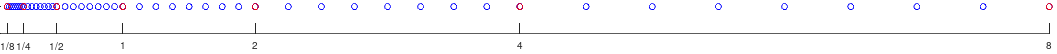
\includegraphics[scale=.4]{escala.png}
\caption{Algunos números positivos de máquina con $b=2$ y $m=4$. Notar que los números son equiespaciados únicamente entre potencias sucesivas de $2$, y que la cantidad de números de máquina en esos rangos se mantiene constante.}
\end{figure}
\begin{tcolorbox}{\bf Distribución de los números de máquina:}
Los números de máquina no se distribuyen de manera uniforme. Describamos dos números de máquina consecutivos  $x_1<x_2$ asumiendo, para simplificar,  que $0<x_1$ y que se escribe:
$$(x_1)_b= 0.b_0b_1b_2...b_{m-1}\, b^{e}.$$
Un momento de reflexión nos dice que el próximo número de máquina (salvo que haya overflow) será
$$(x_2)_b=0.b_0b_1b_2...(b_{m-1}+1)\, b^{e}$$
salvo que $b_{m-1}=b-1$ en cuyo caso
$$(x_2)_b=0.b_0b_1b_2...(b_{m-2}+1)0\, b^{e}$$
salvo que también $b_{m-2}=b-1$ en cuyo caso habrá que repetir el argumento y eventualmente -en caso de que $b_i=b-1$ para todo $0\le i\le m-1$
$$(x_2)_b=0.1b^{e+1}.$$
En cualquier caso observamos que
$$
x_2-x_1=b^{-m}b^e
$$
\emph{no es constante} al variar el exponente $e$, pero sí lo es para cada exponente fijo dado.

\end{tcolorbox}

La consecuencia mas notable de la distribución de los números de máquina es que si $x\in \R$, y existen $x_1<x_2$ números de máquina tales que $x_1\le x\le x_2$ (i.e. $x$ esta dentro de las escalas manejadas por la máquina) entonces
$$
|x-fl_{redond}(x)|\le \frac12 b^{e-m}
$$
$$
|x-fl_{trunc}(x)|\le b^{e-m}
$$
para los casos de redondeo y truncado respectivamente.
\begin{tcolorbox}{\bf Error relativo y precisión de la máquina:}
Nos concentraremos en el caso de redondeo, por lo que asumiremos de aquí en mas que  $fl=fl_{redond}$. Queremos acotar el error relativo al almacenar un número $x\neq 0$.  Observando que
$$b^{e-1}=|0.1\, b^{e}|\le  |x|,$$
resulta
$$
|\frac{x-fl(x)}{x}|\le \frac12 b^{1-m}.
$$
Notar que el error relativo depende \emph{del tamaño de la mantisa}. En el caso de base $b=2$ y $m=52$ mencionado antes resulta:
$$
|\frac{x-fl(x)}{x}|\le  2^{-52}\sim 10^{-16}.
$$
este número, propio de cada máquina, se denomina: precisión de la máquina o épsilon de la máquina y se denota con $\varepsilon$.

En el caso del ejemplo, en terminos simples, dice que nuestra máquina almacena 16 dígitos exactos (en base 10). Naturalemente sería ideal conservar esta precisión a lo largo de las  operaciones que debamos realizar a partir de  $fl(x)$. Eso, como veremos a continuación,  no es posible en general.
\end{tcolorbox}

Como acabamos de ver, en general ocurre que
$x\neq fl(x)$\footnote{Notemos que incluso números muy sencillos como $\frac{1}{10}$ no son de máquina y la introducción de un error de redondeo es inevitable. Evalúe en Python la expresión
$0.1+0.1+0.1!=0.3$, qué obtiene?.}. . Sin embargo podemos garantizar que la diferencia verifica
$$
x-fl(x)=\mu_x x,
$$
con
$$
\frac{|x-fl(x)|}{|x|} =|\mu_x|\le \varepsilon.
$$
Veamos entonces que ocurre con estos errores al efectuar alguna operación
sencilla como por ejemplo sumar. Vamos a distinguir la operación realizada por la máquina con el símbolo $\oplus$.

Pretendemos calcular $x+y$, de modo simplificado la máquina realiza las siguientes operaciones: primero
$$
x\to fl(x) \qquad y\to fl(y)
$$
luego suma $fl(x)+fl(y)$ y finalmente almacena el resultado
$$
fl(x)+fl(y)\to fl(fl(x)+fl(y)).
$$
Cómo se comportará el error resultante?.
Por una lado tenemos:
$$fl(x)=x(1+\mu_x),\qquad  fl(y)=y(1+\mu_y
y),$$ por lo que
$$fl(fl(x)+fl(y))=(fl(x)+fl(y))(1+\mu_z)$$
y en definitiva
$$
x\oplus y =fl(fl(x)+fl(y))=(x(1+\mu_x)+y(1+\mu_y
y))(1+\mu_z).
$$
Vemos entonces que \emph{si $0<x,y$} es posible acotar
$$
|x\oplus y -(x+y)|\le (x+y)2\mu +O(\varepsilon^2)
$$
con $|\mu|\le \varepsilon$. Es decir que hemos de algún modo preservado el tamaño del error relativo\footnote{Cuando los errores se acumulan de forma aditiva, como en este caso, estamos en un buen escenario porque harían falta una enorme cantidad de operaciones para deteriorar el error inicial.}  Como es  bien sabido, eso no es posible si \emph{restamos}
números similares\footnote{Verifique que la cuenta anterior no puede repetirse si los signos de $x$ e $y$ difieren.}.
Un ejemplo elemental es el siguiente: tomemos $b=10$, $m=4$, la precisión es $\varepsilon=\frac{1}{2}10^{-3}=0.0005$. Si $x=125,49$ e $y=125,31$ tenemos respectivamente
$x-y=0.18$
$x\ominus y=0.2$ por lo que el error relativo es
$$
|\frac{x-y-x\ominus y}{x-y}|=\frac{0.02}{0.18}\sim 0.11,
$$
es decir que a pesar de que $\varepsilon \sim 10^{-3}$ el error en la cuenta anterior es del $11\%$. El ejemplo anterior muestra que en una simple operación podemos perder dígitos significativos (de hecho nuestra máquina no ha acertado ningún dígito de la solución). Como regla general deben evitarse restas de números similares\footnote{Ver la guía de ejercicios para mas ejemplos} para evitar la denominada \emph{cancelación catastrófica}.

Es fácil construir ejemplos de números de máquina $0<x<y$ en los cuales no solo $x+y\neq x\oplus y$ sino que, por ejemplo, $x\oplus y=y$. En particular es fácil ver que
\begin{equation}
 \label{eq:epsilonmasuno}
 1 \oplus\varepsilon> 1,
\end{equation}
y
$$
1\oplus\varepsilon/2=1
$$
lo que da una posible definición alternativa del $\epsilon$ como el menor número de máquina con la  propiedad \eqref{eq:epsilonmasuno}.
Otras cuestión que aparece entonces en la aritmética de la máquina es la pérdida de la propiedad asociativa, ya que usando los comentarios previos vemos que por ejemplo
$$
(1\oplus \varepsilon/2)\oplus \varepsilon/2=1\neq 1\oplus (\varepsilon/2+\varepsilon/2).
$$

Hay diversas fuentes de errores computacionales que pueden estropear completamente el resultado de los algoritmos. En este sentido hay dos conceptos que nombraremos tangencialmente ya que no son objeto central de este curso: la \emph{condición} y la \emph{estabilidad}.

De manera muy general, un \emph{problema bien condicionado} es aquél que reacciona benignamente con los errores en los datos. Es decir, que sus soluciones no varían demasiado al no variar demasiado los datos. Por el contrario, si un problema está muy mal condicionado, no lograremos resolverlo con mucha precisión aunque limitemos los errores en los datos (salvo que trabajemos con precisión infinita). La noción de condición es algo \emph{intrínseco del problema} y está mas allá de nuestro algoritmo de resolución \footnote{Un ejemplo concreto y elemental de mal condicionamiento es, como hemos visto, la resta de números similares.} Por otra parte, cuando los problemas están bien condicionados tenemos esperanza de resolverlos con precisión siempre que nuestro algoritmo no incremente desproporcionadamente los errores inherentes a los datos. En este caso hablaramos de \emph{algoritmos estables} y por el contrario, de  \emph{algoritmos inestables} si no cumplen con este criterio. La estabilidad entonces es algo \emph{intrínseco del algoritmo}.




\begin{tcolorbox}
Es posible dar una expresión precisa para la noción de condición, a través del llamado
\emph{número de condición}. Consideremos el problema de evaluar una función en el valor $x_0$. Si por alguna razón (error de medición o redondeo) modificamos el dato a evaluar $x_0$ en un una cierta magnitud pequeña $h$ entonces el error relativo que cometeremos es (asumiendo que la función es de continuamente diferenciable)
$$
\frac{f(x_0+h)-f(x_0)}{f(x_0)}=
\frac{hf'(\eta)}{f(x_0)},$$
para cierto $\eta$ intermedio entre $x_0$ y $x_0+h$. Esto indica que para $h\sim 0$
$$
\frac{hf'(\eta)}{f(x_0)}\sim
\frac{x_0f'(x_0)}{f(x_0)}\frac{h}{x_0}
$$
el error relativo en los datos $\frac{h}{x_0}$ se magnifica en nuestro problema en un factor
$$
\frac{x_0f'(x_0)}{f(x_0)},
$$
llamado el \emph{número de condición} de evaluar $f$ en $x_0$.

\end{tcolorbox}
Como ejemplo de lo anterior
si queremos evaluar $tg(x)$ en un $x_0<\pi/2$, $x_0\sim \pi/2$ vemos que el número de condición
$$
\frac{x_0}{sen(x_0)cos(x_0)},
$$
cumple que
$$
\lim_{x_0\to \pi/2^-} \frac{x_0}{sen(x_0)cos(x_0)}=+\infty.
$$
En particular si elegimos  $x_0$ tal que $\frac{x_0}{sen(x_0)cos(x_0)}\sim 10^{16}$ no esperamos tener ningún dígito significativo en nuestro cálculo de $tg(x_0)$\footnote{Paul Olum, sabiendo que a su amigo Feynmann le gustaba sorprender a todos haciendo cálculos mentales, le pidió un día que aproximara mentalmente $tg(10^{100})$. Feynmann supo al instante que estaba condenado.}.


En los años 50, Wilkinson experimentaba con las primeras computadoras y rápidamente comenzó a observar fenomenos de inestabilidades y mal condicionamiento\footnote{En sus propias palabras: ``The cosy relationship that mathematics enjoyed with polynomials suffered a severe setback in the early fifities where electronic computers came into general use. Speaking for myself I regard it as the most traumatic experience in my carrer as a numerical analyst'' \cite{Wil}  }. Una cosa que notó, al probar un algoritmo de aproximación de raices, es que si al polinomio
$$
p(x)=\prod_{i=1}^{20}(x-i)
$$
se le perturba el coeficiente que acompaña a $x^{19}$ (cuyo valor es $210$ ) en $2^{-23}$ las raíces mayores a $7$ sufren considerables modificaciones. En particular las raices  $10,11,\dots 19$
se transforman en 5 pares complejos conjugados. Las $18$ y $19$ en complejos de la forma $19.5\dots\pm 19.5\dots i$, es decir que una perturbación de orden $2^{-23}$ genera variaciones de orden $1$. \footnote{A pesar de esto, se puede probar que las raíces dependen de forma continua respecto de los coeficientes.} Mostrando que el problema de calcular raices está muy mal condicionado.

Ejemplos de algoritmos inestables abundan. La inestabilidad es muy frecuente y se hace notar muy rápidamente porque los resultados obtenidos difieren notoriamente de lo esperado. Los casos mas extremos aparecen en procesos que deben iterarse en los cuales el error se acumula exponencialmente en vez de aditivamente. Sin embargo hay casos muy simples que pueden ejemplificarse.


Mas arriba vimos que restar números similares es un problema mal condicionado y por eso debe evitarse o tratarse con cautela.

Supongamos que queremos evaluar $e^{-12}$. Usando lo explicado mas arriba, podemos ver que se trata de un problema bien condicionado.  Si utilizamos un algoritmo basado en la serie convergente
$$
e^{-x}=1-x+\frac{1}{2!}x^2-\frac{1}{3!}x^3\cdots
$$
para una evaluación directa en $x=-12$ obtenemos, sumando los primeros 50 términos de la serie:
$$
e^{-12}\sim 6.144189436702122\cdot 10^{-6}.$$
Si por otro lado modificamos el algoritmo calculado primero $e^{12}$
sumando los primeros 50 terminos de la serie
$$
e^{x}=1+x+\frac{1}{2!}x^2+\frac{1}{3!}x^3\cdots
$$
y luego invirtiendo $1/e^{12}$ obtenemos
$$e^{-12}\sim 6.144212353328213\cdot 10^{-6}.$$
La pregunta es a priori, cuál de las dos respuestas es mas confiable. Sin duda el segundo método es mas estable. La razón es que en el cómputo de la serie alternada, muchos terminos ``grandes'' deben cancelarse mágicamente para producir el resultado ``pequeño'' $e^{-12}$. Los errores relativos pequeños son proporcionalmente grandes en términos del resultado final. De hecho
$$e^{-12}\sim 6.1442123533282097586823081788055323112239893148882529755...\cdot 10^{-6}$$
es decir que solo obtuvimos $4$ dígitos correctos con nuestro primero algoritmo pero $14$ con el segundo.
El segundo método es mucho mas estable que el primero.


\begin{tcolorbox}{\bf Puede probar los calculos previos con el algoritmo:}
import numpy as np\\
import math     \\
v=np.arange(0,50)\\
resulI=0.0 \\
resulE=0.0 \\
for i in v:\\

\qquad resulI=resulI+1/math.factorial(i)*(-12.0)**i\\

\qquad resulE=resulE+1/math.factorial(i)*(12.0)**i   \\
resulE=1/resulE \\
print(resulInes)\\
print(resulEs)
\end{tcolorbox}
Los problemas que emergen debido a la precisión limitada de las máquinas dan lugar a muchos comportamientos inesperados. Este último ejemplo, debido a Cleve Moler, es particularmente sencillo y sigue las consideraciones del ejemplo previo. Queremos evaluar $p(x)=(x-1)^7$ para posteriormente graficarlo.
En el primer algoritmo usamos la expresión cerrada $(x-1)^7$  y en el segundo método la expresión equivalente
$$
p(x)=x^7-7x^6+21x^5-35x^4+35x^3-21x^2+7x-1.
$$
En la Figura \ref{fig:moler} a la izquierda vemos ambos gráficos perfectamente superpuestos (azul para el primer método tapado por el rojo del segundo método).
\begin{figure}
 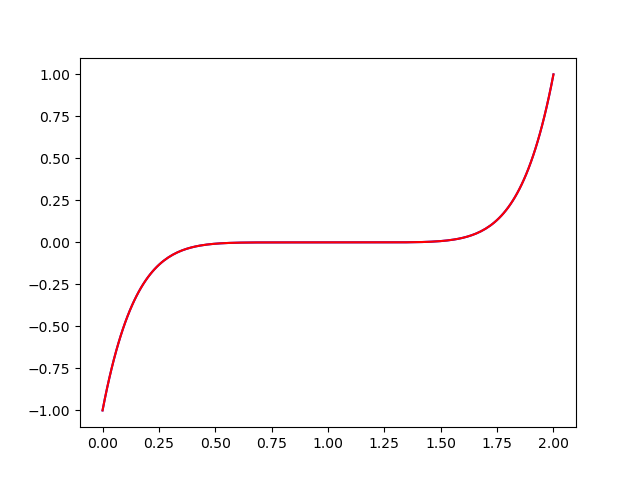
\includegraphics[scale=0.4]{moler1}
 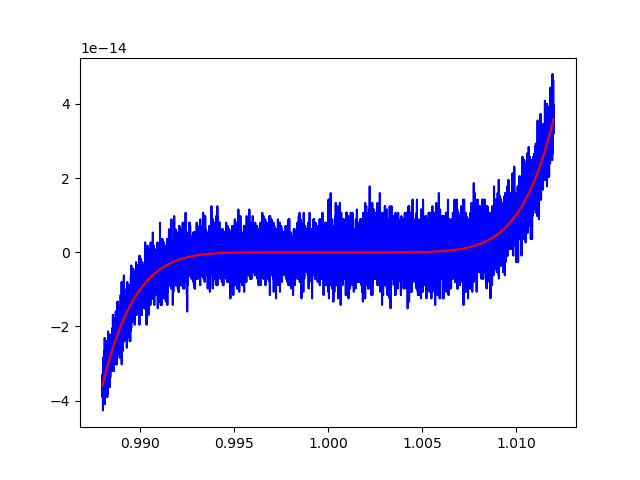
\includegraphics[scale=0.4]{moler2}
 \caption{Gráficos de $p(x)$}
 \label{fig:moler}
 \end{figure}
Sin embargo en la misma figura a la derecha se muestra un zoom cerca de la raíz del polinomio.



Las nociones de condición y estabilidad que hemos comentado de modo superficial son temas transversales a toda el área del análisis  numérico. Como nos restringiremos a cuestiones de álgebra lineal solo hemos pretendido dar una idea somera de sus implicaciones generales. En el capítulo siguiente retomaremos la cuestión de la condición en el ámbito matricial.



\begin{thebibliography}{XXX}

\bibitem{D} J. W. Demmel {\sc Applied Numerical Linear Algebra}
SIAM, 1996.
\bibitem{EN} T. Eirola, O. Nevanlinna, {\sc Numerical Linear Algebra, Iterative Methods}, Lecture Notes, Mat. 1.175, Institute of Mathematics, Helsinki Univ. of Technolgy, 2003.


\bibitem{GVL} G. Golub, C.F. Van Loan, {\sc Matrix Computations}, 3rd. Ed., The Johns Hopkins University Press, 1996.

\bibitem{O} J. M. Ortega,  {\sc Numerical Analysis: A second course.} SIAM, 1990.

\bibitem{TB} L. N. Trefethen, D.Bau III, {\sc Numerical linear algebra}, SIAM 1997.



\bibitem{V} R. S. Varga, {\sc Matrix Iterative Analysis}, Prentice-Hall, 1962.

\bibitem{Wil} J. Wilkinson {\it The perfidious polynomial} Studies in Numerical Analysis, pp. 1-28, MAA Stud. Math., 24, 1984.

\bibitem{HJ} R. Horn, C. Johnson {\it Matrix Analysis}, Cambridge University Press, 1990.

\bibitem{L} S. Lang {\it Algebra}, Springer, 2002.



\end{thebibliography}





\end{document} 
